\documentclass{article}
\usepackage{graphicx}
\usepackage{amsmath}
\PassOptionsToPackage{svgnames}{xcolor}
\usepackage{tcolorbox}
\usepackage{xcolor}
\usepackage{lipsum}
\usepackage{verbatim}
\tcbuselibrary{skins,breakable}
\usetikzlibrary{shadings,shadows}
\usepackage{float}
\usepackage{hyperref}
\usepackage[a4paper]{geometry}
\usepackage{listings}
\usepackage{titlesec}
\usepackage{amssymb}
\usepackage[T1]{fontenc}
\usepackage{multirow} % for Tables
\usepackage{fancyvrb} % for "\Verb" macro
\VerbatimFootnotes % enable use of \Verb in footnotes
\usepackage{listings}
\lstset{basicstyle=\ttfamily,
  showstringspaces=false,
  commentstyle=\color{green},
  keywordstyle=\color{blue}
}

\setcounter{secnumdepth}{4}
\titleformat{\paragraph}
{\normalfont\normalsize\bfseries}{\theparagraph}{1em}{}
\titlespacing*{\paragraph}
{0pt}{3.25ex plus 1ex minus .2ex}{1.5ex plus .2ex}

\title{\textbf{CKA}}
\author{Alejandro Campos}
\date{January, 2023}

\setlength{\parindent}{0ex}
\setlength{\parskip}{6pt}
\geometry{top=2.5cm, bottom=3cm,left=2.5cm, right=2.5cm}
\hypersetup{
    colorlinks=true,
    linkcolor=black,
    filecolor=magenta,      
    urlcolor=blue,
}

\definecolor{codegreen}{rgb}{0,0.6,0}
\definecolor{codegray}{rgb}{0.5,0.5,0.5}
\definecolor{codepurple}{rgb}{0.58,0,0.82}
\definecolor{backcolour}{rgb}{0.95,0.95,0.92}

\newenvironment{blocktemplate}[1]{%
    \tcolorbox[beamer,%
    noparskip,breakable,
    colframe=Blue,%
    colbacklower=LimeGreen!75!LightGreen,%
    title=#1]}%
    {\endtcolorbox}

\newenvironment{blocktemplateI}[1]{%
    \tcolorbox[beamer,%
    noparskip,breakable,
    colframe=Violet,%
    colbacklower=Black,%
    title=#1]}%
    {\endtcolorbox}

\newenvironment{blocktemplateII}[1]{%
    \tcolorbox[beamer,%
    noparskip,breakable,
    colframe=Green,%
    colbacklower=LimeGreen!75!LightGreen,%
    title=#1]}%
    {\endtcolorbox}

\newenvironment{blocktemplateIII}[1]{%
    \tcolorbox[beamer,%
    noparskip,breakable,
    ,colframe=Red,%
    colbacklower=LimeGreen!75!LightGreen,%
    title=#1]}%
    {\endtcolorbox}

\newtcolorbox{mybasecolorbox}[1][]{%
  colback=gray!25, colframe=gray!25,
  coltitle=black,
  width=(\linewidth)}

\newenvironment{codetemplate}[1][]{%
  \mybasecolorbox[#1]
  \itshape
}{%
  \endmybasecolorbox
}

\usepackage{array}

\begin{document}
\maketitle
\newpage
\tableofcontents

%====================================================================================================
\newpage
\section{K8s Core Concepts}

\subsection{High Level Cluster Architecture}

\subsubsection{What is K8s Cluster?}

El objetivo de K8s es alojar aplicaciones en forma de contenedores; para que puedan desplegar facilmente tantos contenedores de la aplicación como sean necesarios y permitir la comunicación entre los diferentes servicios de la aplicación.

Un Cluster de K8s consiste en un conjunto de nodos, que pueden ser físicos o virtuales, que pueden estar desplegados On Premises o en Cloud y que despliegan y gestionan aplicaciones en forma de contenedores.

\subsubsection{Worker Nodes vs Master Node}

Imaginemos un Cluster de K8s como una empresa de barcos, que tiene que albergar contenedores (fisicos) en el mar. Para poder hacer eso, necesitamos barcos de carga que puedan albergar los contenedores, y eso en K8s serían los \textbf{Worker Nodes}. Pero estos barcos tienen que estar gestionados por algún cerebro, en nuestra analogía será el puerto. 

El puerto se encarga de cargar los contenedores en los barcos, planificar como cargarlos para hacerlo eficientemente (sin desperdiciar espacio en los barcos), identificar barcos adecuados para cada tipo de contenedor, albergar información sobre los barcos, controlar y seguir los contenedores en los barcos, etc. Nuestro puerto en K8s es el \textbf{Master Node}.

El \textbf{Master Node} se encarga de gestionar todo el Cluster de K8s almacenando la información relativa a los diferentes nodos, planificando que contenedores van a parar a cada uno de ellos, monitorizando los nodos y los contenedores que en ellos corren, etc. Todo esto lo hace mediante una serie de componentes llamados \textbf{Control Plane}.

\subsubsection{Cluster etcd}

Hay muchisimos contenedores que cargar y descargan en muchisimos barcos, por ello es necesario tener almacenado en algún sitio un registro de: en que barcos se cargan en que contenedores, a que hora, estado de los barcos, estado de los contenedores, etc. Para ello, K8s utiliza un almacén de pares clave-valor de alta disponibilidad \textbf{Cluster etcd}.

\textbf{Cluster Etcd} es una DB que almacena información en formato pares clave-valor.

\subsubsection{Kube-scheduler}

Dentro del puerto, tiene que haber un sistema de gruas que se encargue de gestionar que contenedores se cargan en que barcos, determinar el barco adecuado en función del tamaño del contenedor, capacidad del barco, contenedores que ya lleva cargados, entre otros factores (como el destino del barco, el tipo de contenedores que puede llevar, etc.). De esto, se encarga un elemento dentro del \textbf{Master Node} llamado \textbf{kube-scheduler}.

\textbf{Kube-scheduler} identifica los nodos correctos para alojar cada uno de los contenedores, en función de los recursos necesarios para desplegar el contenedor, la capacidad disponible del nodo, cualquier politica, restricción, regla de afinidad entre nodos, etc.

\subsubsection{Controller Manager}

También, en nuestro puerto, necesitamos un elemento que se encargue del control del estado de los barcos, de las rutas que siguen, los daños que sufren, su estado, si se destruyen... Y poder, en función de este conocimiento, tener otros barcos disponibles donde reubicar los contenedores. Además, este nodo también se encargará de gestionar la comunicación entre los diferentes barcos. 

De estas tareas, se encarga el \textbf{Controller Manager}, compuesto por dos controladores más especificos.

\begin{itemize}
    \item \textbf{Node controller:} se encarga de añadir nuevos nodos en el cluster, gestionar los nodos que ya tiene y gestionar también situaciones de indisponibilidad de nodos, para poder reubicar contenedores.
    
    \item \textbf{Replication Controller:} se encarga de controlar las replicas de contenedores desplegadas en los nodos, garantizando siempre que el numero de replicas deseado se encuentre desplegado entre los diferentes nodos.
\end{itemize}

\subsubsection{Kube-apiserver}

Todo esto está genial, ¿pero como se comunican entre ellos los diferentes elementos de nuestro puerto? ¿Como le dice el \textbf{Replication Controller} al \textbf{kube-scheduler} que necesita cargar un contenedor X que se ha quedado sin barco? ¿Cómo a su vez el \textbf{kube-scheduler} le responde diciendo te lo he metido en este nodo y lo anota en el \textbf{Cluster etcd}? Pues todo eso se hace mediante \textbf{Kube-apiserver}.

\textbf{Kube-apiserver} es el responsable de la orquestación de todas las operaciones dentro del Cluster y además, exponer la \textbf{API de K8s} necesaria para que usuarios externos al Cluster pueden realizar sus operaciones sobre él, así como supervisar el estado del Cluster y realizar las modificaciones que se requieran.

\subsubsection{Todo es containerizable}

Aprovechando las geniales características que nos ofrecen los contenedores, \textbf{todos los elementos del Master Node (control-plane Node)son container-ready}, es decir, pueden desplegarse como servicios containerizados. La solución de red DNS, también puede levantarse como un servicio containerizado. Para ello, necesitamos un software que funcione como motor de construcción y ejecución de esos contenedores, que suele ser \textbf{Docker}, pero K8s también puede utilizar Rocket, o ContainerD. Por tanto, necesitamos \textbf{Docker} (o alternativa) instalado en cada uno de los Nodos del Cluster.s

\subsubsection{Kubelet}

Siguiendo con nuestro ejemplo de empresa naval, cada uno de nuestros barcos tiene un capitán, responsable de la gestión de actividades en los barcos y el que mantiene la conexión con el puerto. Este capitán envía información constante al puerto, indicando si pueden o no albergar nuevos contenedores, el estado en el que se encuentran sus contenedores, la capacidad actual a la que se encuentra el barco... Este capitan en K8s es el \textbf{kubelet}.

\textbf{Kubelet} es un agente que se ejecuta en cada \textbf{Worker} del Cluster, se encarga de recibir las instrucciones del \textbf{kube-apiserver} y desplegar o destruir contenedores en su barco según el \textbf{kube-apiserver} se lo indique. Además se encarga de reportar el estado de su nodo y de los contenedores que se estan ejecutando en el nodo.

Pero estos \textbf{kubelets}, deben poder comunicarse también entre ellos, pues en un nodo puede estar ejecutandose en un contenedor el Front-End de una página web y en otro nodo alejado en otro contenedor el Back-end de la misma, y en otro la DB. ¿Como se comunican los diferentes elementos de una aplicación desplegada en diferentes nodos? Esto se hace mediante el elemento \textbf{kube-proxy}

 El servicio \textbf{kube-proxy} se ejecuta también en cada \textbf{Worker} del Cluster, y se asegura de que existan las reglas a nivel de red necesarias para que los diferentes contenedores de los diferentes workers puedan comunicarse entre si.

 \subsubsection{Worker Nodes vs Master Node (control-plane Node)2}
\begin{table}[H]
\begin{tabular}{| m{5cm} | m{5cm} |}
\hline
\textbf{Master Node} & \textbf{Worker Nodes} \\ \hline
Cluster etcd & kubelets \\
Kube-scheduler & kube-proxy \\
Node controller & \\
Replication Controller & \\
Kube-apiserver & \\ \hline
\end{tabular}
\end{table}

\begin{figure}[H]
    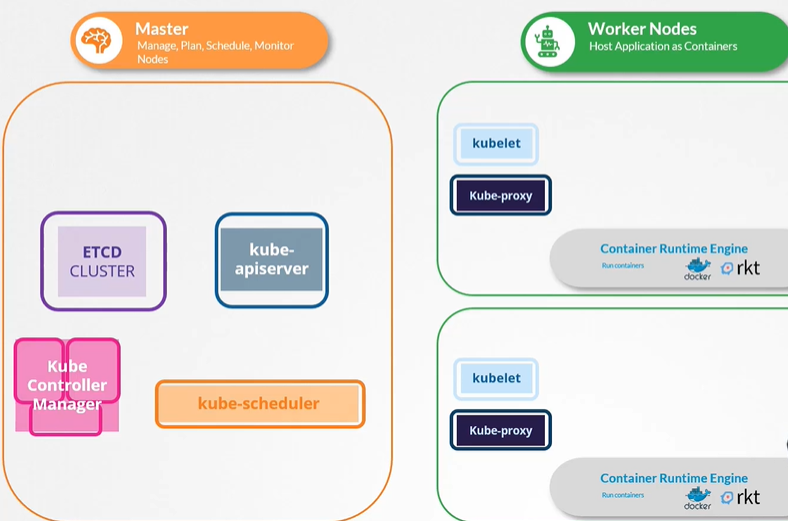
\includegraphics[scale=0.5]{pictures/image.png}
\end{figure}

\subsubsection{High Level Cluster Architecture Picture}

\begin{figure}[H]
    \centering
    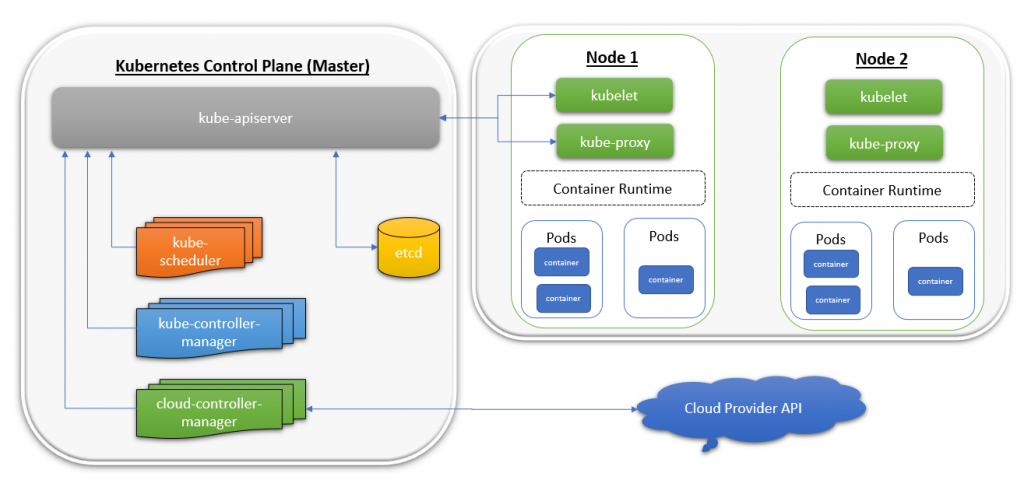
\includegraphics[width=\textwidth]{pictures/image1.png}
    \caption{High Level K8s architecture}
    \label{hlk8s}
\end{figure}

\subsection{Etcd Cluster}

\href{https://kubernetes.io/docs/tasks/administer-cluster/configure-upgrade-etcd/}{Official K8s Doc}

Etcd es una DB que almacena los datos en pares clave-valor y es simple, rápido y seguro.

\subsubsection{What is  key-value store?}

\paragraph{DBS tabulares}

Normalmente, las DBs han tenido un formato  de tabla; como mysql o base de datos relacionales, que almacenan los datos en forma de filas y columnas.

\begin{table}[H]
\begin{tabular}{|m{5em} | m{1cm}|}
\hline
\textbf{name} & \textbf{age} \\ \hline
Alex  & 25 \\
\hline
Claudia & 24 \\
\hline
Mario & 17 \\
\hline
\end{tabular}
\end{table}

Aquí tenemos una imagen de una estructura de base de datos en tabla. Imaginemos que ahora queremos añadir otro campo, como por ejemplo salario. En las DBs en tabla, este campo debe añadirse para todas las entradas, pues se añadirá como columna y todos las filas la tendrán.

\begin{table}[H]
\begin{tabular}{| m{5em} | m{1cm}| m{1.5cm} |}
\hline
\textbf{name} & \textbf{age} & \textbf{salary} \\ \hline
Alex  & 25 & 45k \\
\hline
Claudia & 24 & 31k \\
\hline
Mario & 17 &  \\
\hline
\end{tabular}
\end{table}

Sin embargo, no todos estan trabajando, de forma que la celda de salario de la fila de Mario vacía. Y lo mismo iria pasando con otros campos que vayamos añadiendo

\begin{table}[H]
\begin{tabular}{| m{5em} | m{1cm}| m{1.5cm} | m{1.7cm} |}
\hline
\textbf{name} & \textbf{age} & \textbf{salary} & \textbf{cinturón} \\ \hline
Alex  & 25 & 45k &  \\
\hline
Claudia & 24 & 31k &  \\
\hline
Mario & 17 & & verde  \\
\hline
\end{tabular}
\end{table}

\paragraph{DBS pares clave-valor}

Estas DBs almacenan la información en forma de ficheros o páginas. Así cada entrada tiene asociada un fichero con toda la información acerca de esa entrada. Estos ficheros pueden tener cualquier formato y estructura, aunque suelen utilizarse formatos como \textbf{JSON} o \textbf{YANO}. Los cambios en estos ficheros no afectan a los demás, Claudia y Alex pueden tener información sobre su salario en su fichero y no sobre el cinturón, mientras que Mario a la inversa.

Se pueden añadir detalles adicionales a cada uno de estos ficheros sin tener que actualizar los campos de los demas documentos.

\begin{codetemplate}{alex.json}
\begin{verbatim}
{
   "name": "Alex",
   "age": 25,
   "salary": 45k
}
\end{verbatim}
\end{codetemplate}

\begin{codetemplate}{claudia.json}
\begin{verbatim}
{
   "name": "Claudia",
   "age": 24,
   "salary": 31k
}
\end{verbatim}
\end{codetemplate}

\begin{codetemplate}{mario.json}
\begin{verbatim}
{
   "name": "Mario",
   "age": 17,
   "cinturon": "verde"
}
\end{verbatim}
\end{codetemplate}

\subsubsection{Etcd in Local}

\paragraph{Install etcd:}

We will follow: \href{https://github.com/etcd-io/etcd/releases/}{Github etcd}

\begin{codetemplate}{etcd\_download.sh}
\begin{verbatim}
ETCD_VER=v3.4.26

# choose either URL
GOOGLE_URL=https://storage.googleapis.com/etcd
GITHUB_URL=https://github.com/etcd-io/etcd/releases/download
DOWNLOAD_URL=${GOOGLE_URL}

rm -f /tmp/etcd-${ETCD_VER}-linux-amd64.tar.gz
rm -rf /tmp/etcd-download-test && mkdir -p /tmp/etcd-download-test

curl -L ${DOWNLOAD_URL}/${ETCD_VER}/etcd-${ETCD_VER}-linux-amd64.tar.gz \ 
    -o /tmp/etcd-${ETCD_VER}-linux-amd64.tar.gz
tar xzvf /tmp/etcd-${ETCD_VER}-linux-amd64.tar.gz \
    -C /tmp/etcd-download-test --strip-components=1
rm -f /tmp/etcd-${ETCD_VER}-linux-amd64.tar.gz
\end{verbatim}
\end{codetemplate}

\begin{codetemplate}{}
\begin{verbatim}
$ source etcd_download.sh
\end{verbatim}
\end{codetemplate}

\begin{codetemplate}{}
\begin{verbatim}
$ /tmp/etcd-download-test/etcd --version
\end{verbatim}
\end{codetemplate}

\begin{codetemplate}{}
\begin{verbatim}
$ /tmp/etcd-download-test/etcdctl version
\end{verbatim}
\end{codetemplate}

\textbf{Run etcd Service:}
\begin{codetemplate}{}
\begin{verbatim}
$ /tmp/etcd-download-test/etcd
\end{verbatim}
\end{codetemplate}

\textbf{Etcd service:}

Cuando se ejecuta \textbf{etcd}, se arranca un servicio que escucha en el \textbf{puerto 2379 por defecto}. A continuación puede añadir cualquier cliente al servicio \textbf{etcd} para almacenar y recuperar información.

\paragraph{Etcd controller client (etcdctl)}

Por defecto, etcd service trae incorporade el cliente \textbf{etcdctl}, un cliente que funciona por linea de comandos y que se utiliza para almacenar y recuperar pares clave-valor.

\textbf{Store key-value pairs:} creando una entrada en la DB con la información introducida.
\begin{codetemplate}{}
\begin{verbatim}
$ /tmp/etcd-download-test/etcdctl set key1 value1
\end{verbatim}
\end{codetemplate}

\textbf{Retrieve key-value pairs:}
\begin{codetemplate}{}
\begin{verbatim}
$ /tmp/etcd-download-test/etcdctl get key1
\end{verbatim}
\end{codetemplate}

\textbf{View more options:}
\begin{codetemplate}{}
\begin{verbatim}
$ /tmp/etcd-download-test/etcdctl
\end{verbatim}
\end{codetemplate}

\subsubsection{Etcd in K8s}

Es la DB que almacena todos los datos relativos al cluster, sobre: nodos, PODs, configs, secrets, accounts, roles, ect. Toda la información que nos muestra el comando \verb|kube control get| proviene del servidor etcd. Cada cambio que se produzca en el Cluster: incorporación de nuevos nodos, despliegues de Pods o ReplicaSets, etc. Se actualiza en el servidor etcd, y solo cuando se actualiza en este, se puede considerar que el cambio ha sido completado con éxito.

Dependiendo de como se configure el Cluster, etcd se despliega de forma diferente. A lo largo de esta seccion veremos 2 tipos de despliegue de K8s: uno desplegado desde cero y otro utilizando la herramienta Qadium.

\paragraph{Installing etcd-cluster}

Si has arrancado tu Cluster de K8s utilizando la herramienta \verb|kubeadm|, tu \textbf{etcd-cluster} se generara automaticamente ya configurado. Pero si estás configurando el hardware del Cluster desde cero, entonces el \textbf{etcd-cluster} está disponible como binario en la página de K8s release.

\begin{itemize}
    \item Descargar binario
\begin{codetemplate}{}
\begin{verbatim}
$ wget -q --https-only \ 
"https://github.com/correos/etcd/releases/download/v3.3.9/etcd-v3.3.9-linux-amd64.tar.gz"
\end{verbatim}
\end{codetemplate}

    \item Descomprimir
\begin{codetemplate}{}
\begin{verbatim}
$ tar -xzvf archive.tar.gz -C /path/to/directory/to/extract
\end{verbatim}
\end{codetemplate} 

    \item Una vez descargado puede arrancarse como servicio
\begin{codetemplate}{}
\begin{verbatim}
$ etcd.service
\end{verbatim}
\end{codetemplate}
\end{itemize}

\paragraph{Configuring etcd-cluster}

Hay muchas variables que parametrizan el \textbf{etcd.service} por ahora es importante que nos quedemos con las siguientes: 

\begin{itemize}
    \item dirección donde escucha \textbf{etcd}
\begin{codetemplate}{}
\begin{verbatim}
--advertise-client-urls https://<IP>:2379
\end{verbatim}
\end{codetemplate}

    \item Parametros para garantizar la seguridad de las comunicaciones con certificados \textbf{SSL/ TLS}
\begin{codetemplate}{}
\begin{verbatim}
--cert-file=/etc/etcd/kubernetes.pem
--key-file=/etc/etcd/kubernetes-key.pem
--peer-cert-file=/etc/etcd/kubernetes.pem
--peer-key-file=/etc/etcd/kubernetes-key.pem
...
\end{verbatim}
\end{codetemplate}


\end{itemize}

\paragraph{View etcd-cluster}

Podemos controlar el cluster con el comando \textbf{kubeadm}, y en cuanto al \textbf{etcd}, \textbf{kubeadm} puede desplegar el \textbf{servicio etcd} como un Pod en el namespace del \textbf{Master Node} == \textbf{kube-system namespace}.

\begin{codetemplate}{}
\begin{verbatim}
$ kubectl get pods -n kube-system
    ==> etcd-master
\end{verbatim}
\end{codetemplate}

Para listar todas las claves almacenadas por K8s:

\begin{codetemplate}{}
\begin{verbatim}
$ kubectl exec etcd-master -n kube-system etcdctl get / --prefix -keys-only
\end{verbatim}
\end{codetemplate}

En entornos de alta disponibilidad tendremos varios \textbf{Master Nodes (control-plane Nodes)} dentro del cluster, teniendo también diversas instancias de \textbf{etcd} repartidas entre los \textbf{Master Nodes (control-plane Nodes)}. Para que los diferentes \textbf{etcd} se reconozcan entre ellas debemos configurar en los \textbf{etcd.service} y configurar las diferentes instancias (por url) de los etcd services:

\begin{codetemplate}{}
\begin{verbatim}
-- initial-cluster
\end{verbatim}
\end{codetemplate}

Apart from that, we must also specify path to certificate files so that ETCDCTL can authenticate to the ETCD API Server. The certificate files are available in the etcd-master at the following path. 

\begin{codetemplate}{}
\begin{verbatim}
--cacert /etc/kubernetes/pki/etcd/ca.crt     
--cert /etc/kubernetes/pki/etcd/server.crt     
--key /etc/kubernetes/pki/etcd/server.key
\end{verbatim}
\end{codetemplate}

So to modify that in one command (ETCDCTL API version and path to certificate files):

\begin{codetemplate}{}
\begin{verbatim}
$ kubectl exec etcd-master -n kube-system -- sh -c "ETCDCTL_API=3 etcdctl \ 
    get / --prefix --keys-only --limit=10 \
    --cacert /etc/kubernetes/pki/etcd/ca.crt \
    --cert /etc/kubernetes/pki/etcd/server.crt  \
    --key /etc/kubernetes/pki/etcd/server.key"
\end{verbatim}
\end{codetemplate}

\paragraph{Etcd commands}

\textbf{API Version 2}

\begin{codetemplate}{}
\begin{verbatim}
etcdctl backup
etcdctl cluster-health
etcdctl mk
etcdctl mkdir
etcdctl set
\end{verbatim}
\end{codetemplate}

\textbf{API Version 2}

\begin{codetemplate}{}
\begin{verbatim}
etcdctl snapshot save 
etcdctl endpoint health
etcdctl get
etcdctl put
\end{verbatim}
\end{codetemplate}

To set the right version of ETCDCTL API set the environment variable ETCDCTL\_API command, so when API version is not set, it is assumed to be set to version 2:

\begin{codetemplate}{}
\begin{verbatim}
$ export ETCDCTL_API=3
\end{verbatim}
\end{codetemplate}

\subsection{Kube API Server}

\href{https://kubernetes.io/docs/reference/command-line-tools-reference/kube-apiserver/}{Official K8s Doc}

Principal componente de gestión de K8s. Cuando se ejecuta un comando \textbf{kubectl}, este llega al \textbf{kube-apiserver}, y este primero autentifica la solicitud y la valida. A continuación recupera la información del \textbf{etcd-cluster} y responde con la información.

Pongamos el ejemplo de la creación de un Pod:

\begin{enumerate}
    \item \textbf{kubectl} create pod.yaml
    \item \textbf{kube-apiserver} crea un Pod sin asignarlo a ningun nodo, consolida esta información en el \textbf{etcd-cluster} y reporta al usuario que ya lo ha creado
    \item \textbf{kube-scheduler} monitoriza constantemente el \textbf{kube-apiserver} y se da cuenta de que se ha creado un nuevo Pod sin nodo asignado.
    \item \textbf{kube-scheduler} busca el nodo adecuado para hostear el Pod y se lo comunica al \textbf{kube-apiserver}
    \item \textbf{kube-apiserver} actualiza la información en el \textbf{etcd-cluster} y contacta con el \textbf{kubelet} del \textbf{worker} correspondiente.
    \item El \textbf{kubelet} del \textbf{worker} seleccionado crea el Pod y contacta con el \textbf{container runtime} para que despliegue en el la imagen de la aplicación.
    \item Una vez hecho, el \textbf{kubelet} actualiza el estado del Pod al \textbf{kube-apiserver} y este actualiza los datos en el \textbf{etcd-cluster}
    
\end{enumerate}

Para todas las peticiones kubectl sobre el Cluster se sigue un patrón similar, el \textbf{kube-apiserver} gestiona todas las diferentes tareas que hay que realizar para llevar a cabo un cambio en el Cluster, como se puede ver en la Figura \ref{hlk8s}.



\begin{blocktemplateII}{Note}
El \textbf{kube-apiserver} es el responsable de autenticar y validar todas las solicitudes por \textbf{kubectl} y actualizar los datos en el \textbf{etcd-cluster}. De echo \textbf{kube-apiserver} es el único componente que puede interactuar directamente con el \textbf{etcd-cluster}. Los otros elementos como el \textbf{kube-scheduler}, el \textbf{kube-controller-manager} o los \textbf{kubelet} utilizan el \textbf{kube-apiserver} como intermediario para actualizar los datos en el \textbf{etcd-cluster}. Es una forma de evitar la inconsistencia de datos gestionando la concurrencia desde el \textbf{kube-apiserver}.
\end{blocktemplateII}


\subsubsection{Kube-apiserver in K8s}

\paragraph{Installing kube-apiserver}

Si has arrancado tu Cluster de K8s utilizando la herramienta \verb|kubeadm|, tu \textbf{kube-apiserver} se generara automaticamente ya configurado. Pero si estás configurando el hardware del Cluster desde cero, entonces el \textbf{kube-apiserver} está disponible como binario en la página de K8s release.

\begin{itemize}
    \item Descargar binario
\begin{codetemplate}{}
\begin{verbatim}
$ wget https://storage.googleapis.com/kubernetes-release/release/
    v1.13.0/bin/linux/amd64/kube-apiserver
\end{verbatim}
\end{codetemplate}

    \item Descomprimir
\begin{codetemplate}{}
\begin{verbatim}
$ tar -xzvf archive.tar.gz -C /path/to/directory/to/extract
\end{verbatim}
\end{codetemplate} 

    \item Una vez descargado puede arrancarse como servicio
\begin{codetemplate}{}
\begin{verbatim}
$ kube-apiserver.service
\end{verbatim}
\end{codetemplate}
\end{itemize}

Se puede descargar y configurar para que se ejecute como un servicio en el \textbf{Master Node} de tu Cluster. El \textbf{kube-apiserver} se configura con muchos parametros, esto se explica ya que un Cluster de k8s son un monton de componentes diferentes que trabajan juntos, comunicandose entre ellos de muchas maneras diferentes, así que todos deben saber donde se encuentran los demás componentes. Además, existen diferentes modos de autenticación, autorización, cifrado, seguridad, etc. Es por eso que cada componente del cluster requiere tantos parametros de configuración.

\paragraph{Parametros importantes}

\begin{blocktemplate}{Note}
\label{SSLCerts}
Como todos los componentes se comunican entre ellos, todos ellos tendran configurable una sección de parametros para garantizar la seguridad de las comunicaciones, con certificados \textbf{SSL/ TLS}
\end{blocktemplate}

\begin{itemize}
    \item Parametros para garantizar la seguridad de las comunicaciones entre los diferentes componentes, con certificados \textbf{SSL/ TLS}
\begin{codetemplate}{}
\begin{verbatim}
--etcd-cafile=/var/lib/kubernetes/ca.pem
--etcd-certfile=/var/lib/kubernetes/kubernetes.pem
--etcd-keyfile=/var/lib/kubernetes/kubernetes-key.pem
\end{verbatim}
\end{codetemplate}

    \item Cadena de conexión contra \textbf{etcd-servers}
\begin{codetemplate}{}
\begin{verbatim}
--etcd-servers=https://127.0.0.1:2379
\end{verbatim}
\end{codetemplate}
\end{itemize}

\paragraph{View kube-apiserver}

\textbf{Con kubeadm}

\begin{itemize}
    \item Si lo hemos levantado con \verb|kubeadm| tool el \textbf{kube-apiserver} estará desplegado como un Pod dentro del namespace del \textbf{Master Node} == \textbf{kube-system namespace}:
\begin{codetemplate}{}
\begin{verbatim}
$ kubectl get pods -n kube-system
    ==> kube-apiserver-master
\end{verbatim}
\end{codetemplate}

     \item También lo podremos ver accediendo a su yaml dentro del directorio \verb|/etc/kubernetes/manifests/|:
\begin{codetemplate}{}
\begin{verbatim}
$ cat /etc/kubernetes/manifests/kube-apiserver.yaml
\end{verbatim}
\end{codetemplate}
\end{itemize}

\textbf{Sin kubeadm}
\begin{itemize}
    \item Si no hemos utilizado \verb|kubeadm| para levantar el Cluster de K8s, podemos ver las opciones accediendo a la definición del servicio en el sistema \verb|/etc/systemd/system/kube-apiserver.service|:
\begin{codetemplate}{}
\begin{verbatim}
$ cat /etc/systemd/system/kube-apiserver.service
\end{verbatim}
\end{codetemplate}

    \item También encontrarlo en la lista de tareas en ejecución de tu sistema si tienes el cluster levantado:
\begin{codetemplate}{}
\begin{verbatim}
$ ps -aux | grep kube-apiserver
\end{verbatim}
\end{codetemplate}
\end{itemize}

\subsection{Kube Controller Manager}

\href{https://kubernetes.io/docs/reference/command-line-tools-reference/kube-controller-manager/}{Official K8s Doc}

El \textbf{kube-controller-manager} gestiona diferentes controladores en K8s. Un controlador en K8s es como una oficina o departamento dentro del puerto que tiene su propio conjunto de responsabilidades, las cuales deben estar constantemente pendientes del estado de los \textbf{worker} y tomando las acciones necesarias para remediar la situación.

En definición K8s, un controlador es un proceso que supervisa constantemente el estado de varios componentes en el sistema y trabaja para llevar todo el sistema al estado de funcionamiento deseado.

Los diferentes controladores que gestiona el \textbf{Kube Controller Manager} son:

\begin{itemize}
    \item Node-Controller
    \item Replication-Controller
    \item Namespace-Controller
    \item Deployment-Controller
    \item Job-Controller
    \item PV-Protection-Controller
    \item Service-Account-Controller
    \item ...
\end{itemize}

\subsubsection{Node-Controller}
El \textbf{Node-controller} se encarga de supervisar el estado de los nodos y tomar las acciones necesarias para mantener los Pods corriendo. Esto lo hace comunicandose con el \textbf{kube-apiserver}, preguntando por el estado de todos nodos cada 5 segundos. Si un nodo deja de responder durante 40 segundos este se marca como \textbf{unreachabl}e por el \textbf{node-controller}.

Una vez un nodo ha sido marcado como \textbf{unreachable}, le da 5 minutos para recuperarse, si no lo hace, elimina los Pods asignados a ese worker y los aprovisiona en otros nodos saludables.

\subsubsection{Replication-Controller}
Se encarga de supervisar el estado de los diferentes \textbf{ReplicaSets}, comprobando en cada momento que haya desplegados en el cluster el numero de Pods disponibles indicados por el ReplicaSet. Si un Pod muere, crea otro.

\subsubsection{Kube-Controller-Manager in K8s}

¿Como podemos ver todos estos controladores y donde estan ubicados en el Cluster? Todos ellos estan empaquetados bajo un solo proceso, \textbf{Kube-Controller-Manager}. De forma que si nos descargamos e instalamos \textbf{Kube-Controller-Manager}, estaremos descargando e instalando con el todos los controladores necesarios para el correcto funcionamiento de K8s.

\paragraph{Install Kube-Controller-Manager}

Si has arrancado tu Cluster de K8s utilizando la herramienta \verb|kubeadm|, tu \textbf{kube-controller-manager} se generara automaticamente ya configurado. Pero si estás configurando el hardware del Cluster desde cero, entonces el \textbf{kube-controller-manager} está disponible como binario en la página de K8s release.

\begin{itemize}
    \item Descargar binario
\begin{codetemplate}{}
\begin{verbatim}
$ wget https://storage.googleapis.com/kubernetes-release/release/
    v1.13.0/bin/linux/amd64/kube-controller-man
\end{verbatim}
\end{codetemplate}

    \item Descomprimir
\begin{codetemplate}{}
\begin{verbatim}
$ tar -xzvf archive.tar.gz -C /path/to/directory/to/extract
\end{verbatim}
\end{codetemplate} 

    \item Una vez descargado puede arrancarse como servicio
\begin{codetemplate}{}
\begin{verbatim}
$ kube-controller-manager.service
\end{verbatim}
\end{codetemplate}
\end{itemize}

\paragraph{Configure Kube-Controller-Manager}

Como con todos los elementos, tiene una larga lista de parametros configurables. Por aquí dejo algunos relevantes (no voy a nombrar más los de certificados, que este, como todos los elemntos, tambien necesita, sección \ref{SSLCerts}).

\begin{codetemplate}{}
\begin{verbatim}
--node-monitor-period=5s
--node-monitor-grace-period=40s
--pod-eviction-timeout=5m0s
--controllers
\end{verbatim}
\end{codetemplate}

En la sección de controllers pueden especificarse los controladores que queremos tener habilitados, por defecto lo estan todos.

En caso de que alguno de los controladores no parezca funcionar o no exista, este sería un buen punto de partida donde mirar.

\paragraph{View Kube-Controller-Manager}

\textbf{Con kubeadm}

\begin{itemize}
    \item Como siempre, si levantamos nuestro Cluster con \verb|kubeadm|, el \textbf{kube-controller-manager} se levanta como un Pod en el namespace del \textbf{Master Node} == \textbf{kube-system namespace}:
\begin{codetemplate}{}
\begin{verbatim}
$ kubectl get pods -n kube-system
    ==> kube-controller-manager-master
\end{verbatim}
\end{codetemplate}

    \item También puedes acceder a su manifest dentro de la carpeta que \verb|kubeadm| utiliza para desplegar estos Pods:
\begin{codetemplate}{}
\begin{verbatim}
cat /etc/kubernetes/manifests/kube-controller-manager.yaml
\end{verbatim}
\end{codetemplate}
\end{itemize}

\textbf{Sin kubeadm}

\begin{itemize}
    \item Como siempre también, puedes inspeccionar las opciones viendo el servicio en si ejecutandose por el sistema:
\begin{codetemplate}{}
\begin{verbatim}
cat /etc/systemd/system/kube-controller-manager.service
\end{verbatim}
\end{codetemplate}

    \item O filtrando su nombre en todos los servicios de ejecución del sistema:
\begin{codetemplate}{}
\begin{verbatim}
$ ps -aux | grep kube-controller-manager
\end{verbatim}
\end{codetemplate}
\end{itemize}

\subsection{Kube Scheduler}

\href{https://kubernetes.io/docs/reference/command-line-tools-reference/kube-scheduler/}{Official K8s Doc}

\textbf{K8s Scheduler} es el encargado de programar los Pods en los nodos, de decidir que Pod va en cada nodo. Pero no crea los pods en los nodos, ya que esto es tarea del kubelet. El \textbf{kube-scheduler} simplemente decide en que worker debe crearse cada pod.

\subsubsection{How does kube-scheduler work?}

Cuando hay muchos nodos y muchos Pods diferentes, hay que asegurarse de que el Pod en concreto puede levantarse en otro nodo concreto, dependiendo de algunas características especificas del Pod, pero sobretodo basandose en los requisitos de recursos del Pod y capacidad disponible del nodo.

Para ello, el \textbf{kube-scheduler} crea 2 etapas de filtros:

\label{Scheduling}
\begin{enumerate}
    \item Descarta aquellos Nodos en los cuales el Pod no puede desplegar, por caraterísticas definidas de ambos que veremos más adelante.
    \item Descarta aquellos nodos con menos capacidad disponible de los recursos que requiere el Pod para desplegar (required).
    \item Dentro de los nodos con suficiente capacidad como para levantar el Pod busca aquel con mayor capacidad sobrante una vez desplegado el Pod con sus requirements de recursos. Aquel nodo al que le sobre más capacidad es el que finalmente levanta el Pod.
\end{enumerate}

\subsubsection{Kube-Scheduler in K8s}
\label{schduler}

\paragraph{Install Kube-Scheduler}

Si has arrancado tu Cluster de K8s utilizando la herramienta \verb|kubeadm|, tu \textbf{kube-scheduler} se generara automaticamente ya configurado. Pero si estás configurando el hardware del Cluster desde cero, entonces el \textbf{kube-scheduler} está disponible como binario en la página de K8s release.

\begin{itemize}
    \item Descargar binario
\begin{codetemplate}{}
\begin{verbatim}
$ wget https://storage.googleapis.com/kubernetes-release/release/
    v1.13.0/bin/linux/amd64/kube-scheduler
\end{verbatim}
\end{codetemplate}

    \item Descomprimir
\begin{codetemplate}{}
\begin{verbatim}
$ tar -xzvf archive.tar.gz -C /path/to/directory/to/extract
\end{verbatim}
\end{codetemplate} 

    \item Una vez descargado puede arrancarse como servicio
\begin{codetemplate}{}
\begin{verbatim}
$ kube-scheduler.service
\end{verbatim}
\end{codetemplate}
\end{itemize}

\paragraph{Kube-Scheduler options}

\textbf{kubeadm}

\begin{itemize}
    \item Como siempre, si levantamos nuestro Cluster con \verb|kubeadm|, el \textbf{kube-scheduler} se levanta como un Pod en el namespace del \textbf{Master Node} == \textbf{kube-system namespace}:
\begin{codetemplate}{}
\begin{verbatim}
$ kubectl get pods -n kube-system
    ==> kube-scheduler-master
\end{verbatim}
\end{codetemplate}

    \item También puedes acceder a su manifest dentro de la carpeta que \verb|kubeadm| utiliza para desplegar estos pods:
\begin{codetemplate}{}
\begin{verbatim}
cat /etc/kubernetes/manifests/kube-scheduler.yaml
\end{verbatim}
\end{codetemplate}
\end{itemize}

\textbf{kubeadm}

\begin{itemize}
    \item Como siempre también, puedes inspeccionar las opciones viendo el servicio en si ejecutandose por el sistema:
\begin{codetemplate}{}
\begin{verbatim}
cat /etc/systemd/system/kube-scheduler.service
\end{verbatim}
\end{codetemplate}

    \item O filtrando su nombre en todos los servicios de ejecución del sistema:
\begin{codetemplate}{}
\begin{verbatim}
$ ps -aux | grep kube-scheduler
\end{verbatim}
\end{codetemplate}
\end{itemize}

\subsection{Kubelet}

\href{https://kubernetes.io/docs/reference/command-line-tools-reference/kubelet/}{Official K8s Doc}

Es el capitan del barco (Worker Node), es quien carga los contenedores en los barcos (está mamadisimo) según las instrucciones del \textbf{kube-scheduler}, está comunicandose constantemente con el \textbf{kube-apiserver} y con el resto de \textbf{kubelets} enviando informes constantes sobre el estado del barco y los contenedores que este alberga, además es quien regitra el nodo en un cluster de K8s.

Cuando le llega una orden directa del \textbf{kube-scheduler} (pasando siempre por el \textbf{kube-apiserver}) de levantar un pod, el \textbf{kubelet} es el encargado de contactar con el motor de containerización para que extraiga la imagen necesaria y ejecute una instancia dentro de un pod.

El \textbf{kubelet} constantemente monitoriza el estado de los pods y los contenedores que este contiene, enviando informes constantes al \textbf{kube-apiserver}

\subsubsection{kubelet in K8s}

\paragraph{Install kubelet}

El kubelet está disponible como binario en la página de K8s release.

Si has arrancado tu Cluster de K8s utilizando la herramienta \verb|kubeadm|, tu \textbf{kubelet} se generara automaticamente ya configurado. Pero si estás configurando el hardware del Cluster desde cero, entonces el \textbf{kubelet} está disponible como binario en la página de K8s release.

\begin{itemize}
    \item Descargar binario
\begin{codetemplate}{}
\begin{verbatim}
$ wget https://storage.googleapis.com/kubernetes-release/release/
    v1.13.0/bin/linux/amd64/kubelet
\end{verbatim}
\end{codetemplate}

    \item Descomprimir
\begin{codetemplate}{}
\begin{verbatim}
$ tar -xzvf archive.tar.gz -C /path/to/directory/to/extract
\end{verbatim}
\end{codetemplate} 

    \item Una vez descargado puede arrancarse como servicio
\begin{codetemplate}{}
\begin{verbatim}
$ kubelet.service
\end{verbatim}
\end{codetemplate}
\end{itemize}

\begin{blocktemplateIII}{Warning}
Si hemos levantado nuestro cluster de K8s con \verb|kubeadm|, este NO levanta automáticamente kubelets. \textbf{SIEMPRE debes instalar el kubelet en tus Worker Nodes}
\end{blocktemplateIII}

Una vez descargado podemos correrlo como un servicio:

\begin{codetemplate}{}
\begin{verbatim}
$ kubelet.service
\end{verbatim}
\end{codetemplate}

\paragraph{kubelet options}

\begin{itemize}
    \item Puedes inspeccionar las opciones viendo el servicio en si ejecutandose por el sistema:
\begin{codetemplate}{}
\begin{verbatim}
cat /etc/systemd/system/kubelet.service
\end{verbatim}
\end{codetemplate}

    \item O filtrando su nombre en todos los servicios de ejecución del sistema:
\begin{codetemplate}{}
\begin{verbatim}
$ ps -aux | grep kubelet
\end{verbatim}
\end{codetemplate}
\end{itemize}

\subsection{Kube Proxy}

\href{https://kubernetes.io/docs/reference/command-line-tools-reference/kube-proxy/}{Official K8s Doc}

Dentro de un cluster de K8s, todos los pods pueden conectarse con todos los demás pods. Esto es posible gracias al despliegue de un red de pods en el cluster. Esta red, es una \textbf{red virtual interna}, que se extiende por todos los nodos del cluster para tener todos los pods conectados. Gracias a esta red, todos los nodos son capaces de comunicarse entre ellos.

Un ejemplo de necesidad de esta red es una aplicación web sencilla que funciona con un front-end y una DB. El Pod que corre el front-end está desplegado en un Nodo A, en una punta del cluster, mientras que  el Pod que corre la DB está desplegado en un Nodo B, en la otra punta del cluster. ¿Como se comunican entre ellos? ¿Cuando el front-end necesita información de la DB para mostrar? 

Si no tubieramos ni idea de K8s, podríamos decir que asociando a nuestro fron-end la IP del Pod de la DB, pero esto sería un error. Porque no podemos asegurar que el IP del Pod de DB sea siempre la misma, ya que en caso de reinicio la IP del Pod cambiará.

La mejor forma de que el Pod de front-end se comunique con la DB es a traves de los \textbf{Services}. Los \textbf{Servicios} en K8s nos exponen las aplicaciones mediante el nombre del servicio o su IP y las hacen accesibles dentro del Cluster, desde cualquier lugar o parte dentro del mismo.

Así pues, el Front-end podrá llegar a la DB utilizando el nombre del \textbf{Service}. El \textbf{Service} también tiene una IP asignada. Pero entonces... ¿Puede el servicio desplegarse como un Pod y añadirse a esta red interna? La respuesta es NO, pues el \textbf{Service} no es una cosa real, no ejecuta ningún contenedor como los Pods, no tiene un proceso de escucha activa, es un elemento virtual que solo vive en la memoria de K8s.

Estos \textbf{Services} deben ser accesibles desde cualquier nodo del Cluster, ¿como conseguimos eso? Aquí es donde entre al \textbf{Kube-proxy}, un proceso que se ejecuta en cada nodo del Cluster de K8s, su trabajo es buscar nuevos servicios, y cada vez que encuentra un nuevo servicio, crea las reglas necesarias en cada \textbf{Worker Node} para poder reenviar trafico de los nuevos servicios a los Pods. Una de las formas de hacerlo es mediante \textbf{IPtables roules}. En este caso, \textbf{Kube-proxy} crea una regla \textbf{iptable} en cada nodo del cluster para reenviar el tráfico desde la IP del service hacia la ip del pod.

\begin{figure}[H]
    \centering
    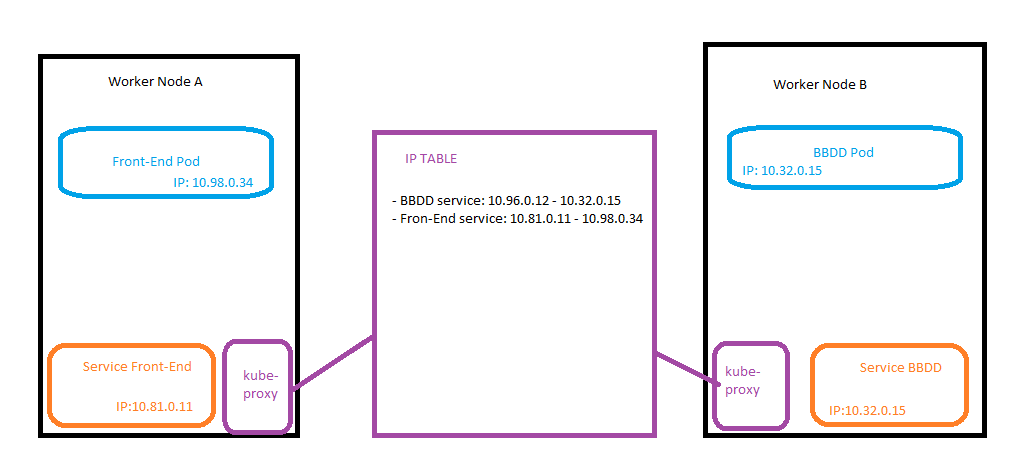
\includegraphics[scale=0.4]{pictures/image2.png}
\end{figure}

\subsubsection{kube-proxy in K8s}

\paragraph{Install kube-proxy}

Si has arrancado tu Cluster de K8s utilizando la herramienta \verb|kubeadm|, tu \textbf{kube-proxy} se generara automaticamente ya configurado. Pero si estás configurando el hardware del Cluster desde cero, entonces el \textbf{kube-proxy} está disponible como binario en la página de K8s release.

\begin{itemize}
    \item Download binary
\begin{codetemplate}{}
\begin{verbatim}
$ wget https://storage.googleapis.com/kubernetes-release/release/
    v1.13.0/bin/linux/amd64/kube-proxy
\end{verbatim}
\end{codetemplate}

    \item Unpackage it
\begin{codetemplate}{}
\begin{verbatim}
$ tar -xzvf archive.tar.gz -C /path/to/directory/to/extract
\end{verbatim}
\end{codetemplate} 

    \item Once downloaded and unpackaged it can be run as a service
\begin{codetemplate}{}
\begin{verbatim}
$ kube-proxy.service
\end{verbatim}
\end{codetemplate}
\end{itemize}

\paragraph{kube-proxy options}

\textbf{With kubeadm}

\begin{blocktemplateI} {Note}
If K8s Cluster is setup with \verb|kubeadm|, \textbf{kube-proxy} it deploys as \textbf{DaemonSet}. That means that a \textbf{kube-proxy} Pod will be deployed on every Node of the K8s Cluster. Without \verb|kubeadm| it should be done it by hand.
\end{blocktemplateI}

\begin{itemize}
    \item If K8s Cluster is setup with \verb|kubeadm|, \textbf{kube-proxy} runs as Pod in every Node of K8s Cluster as \textbf{DaemonSet}
\begin{codetemplate}{}
\begin{verbatim}
$ kubectl get daemonset -n kube-system
    ==> kube-proxy
\end{verbatim}
\end{codetemplate}

    \item También puedes acceder a su manifest dentro de la carpeta que \verb|kubeadm| utiliza para desplegar estos pods:
\begin{codetemplate}{}
\begin{verbatim}
cat /etc/kubernetes/manifests/kube-proxy.yaml
\end{verbatim}
\end{codetemplate}
\end{itemize}

\textbf{Sin kubeadm}

\begin{itemize}
    \item Como siempre también, puedes inspeccionar las opciones viendo el servicio en si ejecutandose por el sistema:
\begin{codetemplate}{}
\begin{verbatim}
cat /etc/systemd/system/kube-proxy.service
\end{verbatim}
\end{codetemplate}

    \item O filtrando su nombre en todos los servicios de ejecución del sistema:
\begin{codetemplate}{}
\begin{verbatim}
$ ps -aux | grep kube-proxy
\end{verbatim}
\end{codetemplate}
\end{itemize}

%===============================================================
\newpage
\section{Core Resources}
\subsection{Pods}

\href{https://kubernetes.io/docs/concepts/workloads/pods/}{Official K8s Doc}

\begin{blocktemplate}{Note}
In order to start explaining pods, we assume the following:

\begin{itemize}
    \item The application is already developed and built into Docker image.
    \item The image is available on a Docker repository (for example Docker Hub), so K8s can pull it down.
    \item Also assume the K8s Cluster is already setup, configured and correctly working. It could be configured as a single-node setup (as in our PC local cluster) or a multi-node setup (like ICP).
\end{itemize}
\end{blocktemplate}

\subsubsection{Pod, a single instance of an app}

As we discuss before, with K8s our ultimate aim is to deploy our application in the form of containers on a set of machines that are configured as worker Nodes inside the K8s Cluster. However \textbf{K8s does not deploy containers directly on the worker Nodes, the container are encapsulated into a K8s Object known as Pods}.

A Pod is a single instance of an application, a Pod is the smallest object we can create in K8s. Let's see an example:

\underline{EXAMPLE:}

Imagine that we have the simplest K8s cluster, with only one Node, and one Pod running an application container.

\textbf{1. What happens if the number of users starts to increase?}

\begin{itemize}
    \item \textcolor{red}{Bad answer:} start another container inside the Pod
    \item \textcolor{green}{Good answer:} create a new Pod with a new instance of the same application
\end{itemize}

\begin{figure}[H]
    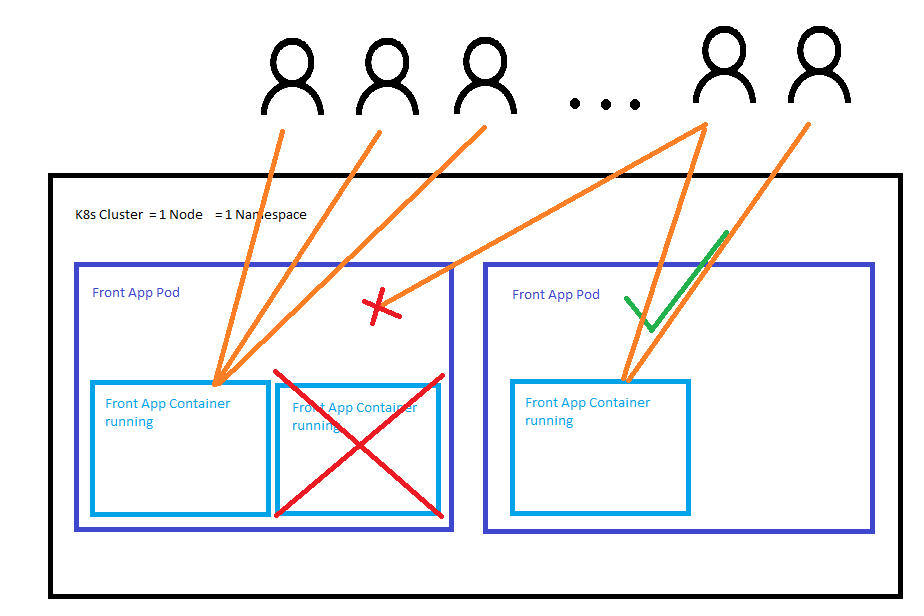
\includegraphics[scale=0.5]{pictures/image3.png}
\end{figure}

\textbf{What happens if the Node has not enough capacity?}

It can be created new pods witha new instance of the same application on another Nodes inside the Cluster. So we should add new Nodes to expand the cluster's physical capacity.

\begin{blocktemplate}{Note}
What is important to remark, is that is a best practice to have a one-to-one relationship between containers and running aplications. To scale up, we create new pods, not new containers in the Pods. And to scale down, just remove those pods.
\end{blocktemplate}


\subsubsection{Multi-Container Pod}

We said it is a best practise to have one-to-one relationship between Pods and application. But sometimes, the applications need to run two or more containers in the same Pod, a helper container which might be doing some kind of supporting task for our application (for example to run a healthcheck solution to expose the state of the app). And we want these helper containers to run alongside application main process (the main cotainer). For that cases, multi-container Pods can be created, because Pods can run multiple containers.

But we must know, that the scalation will be for the two containers, we cannot scale up the main application without scaling up the side-car container too. And if the main container has some problem and it dies, both container dies, since they are part of the same pod.

\begin{blocktemplateII}{Note}
The two containers can also communicate with each other directly by referring to each other as \textbf{localhost}, since they share the same network space. Plus, they can easily share the same storage space as well.    
\end{blocktemplateII}

\subsubsection{Helping containerization life cycle}

Imagine we don't have K8s, we just have docker, and we want to containerize and run our application. we should use the docker run command to do it.

\begin{codetemplate}{}
\begin{verbatim}
$ docker run python-app
\end{verbatim}
\end{codetemplate}


If the load increases we deploy more instances of our application:

\begin{figure}[H]
    \centering
    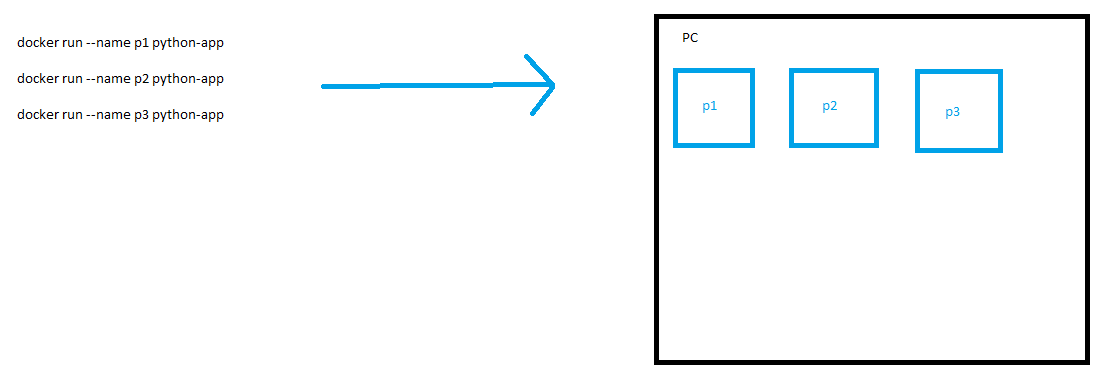
\includegraphics[scale=0.4]{pictures/image4.png}
\end{figure}

If our architecture grows and gets complex, for example our application uses a DB. We now have to run a new DB container linked to out web application. They must have a one-to-one relationship.

\begin{figure}[H]
    \centering
    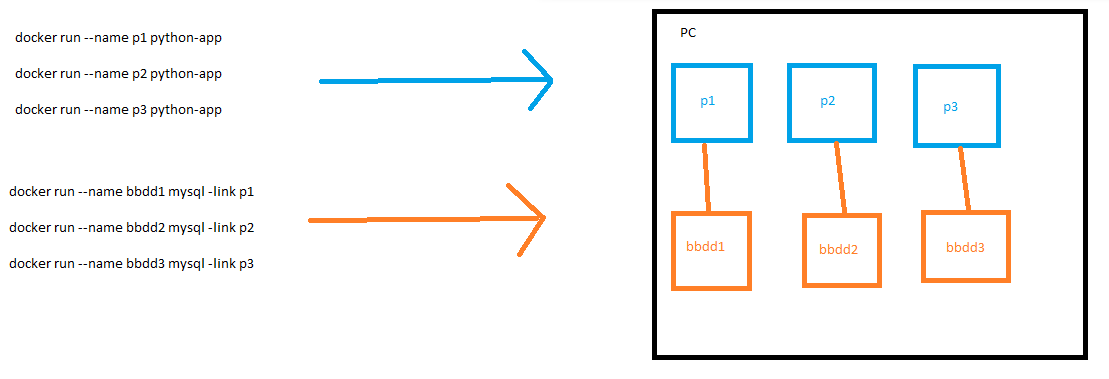
\includegraphics[scale=0.55]{pictures/image5.png}
\end{figure}

To maintain this infrastructure in docker, it is needed to establish the Network Connectivity and configuration to enable these communications, we would need to establish persistent storage to share it among the containers, we would need to maintain a communication map and storage map. And the most important, we would need to monitor the state of the application container and when it dies, kill the helper container as well as it is no longer required. And when a new container of the app is deployed, a new container of DB should be deployed as well.

\begin{blocktemplateI}{Note}
Maybe the DB example is not quite good, because it is better to run DB on another Pod, but imagine it is another service less detachable, for example healthcheck, or a service to do something for the main application.
\end{blocktemplateI}

With Pods, K8s makes all these tasks for us automatically, we just need to define what containers a Pod consists off and the containers ia Pod by default will have access to the same Network and Storage. Also they will be created together and destroyed together.

Even the application is simple and it doesn't need to run more than one container K8s still requires to create pods. However multi-container Pods are rare, so we will focus in single containers per Pod in this course.

\subsubsection{How to easily deploy a basic Pod}

\begin{codetemplate}{}
\begin{verbatim}
$ kubectl run nginx-pod --image nginx
\end{verbatim}
\end{codetemplate}

It deploys a Docker container by creating a Pod in the current namespace. So in this case, it creates at first a Pod automatically (called nginx-pod) and then it deploys an instance of the NGINX Docker image. But where does it get the application image from? If nothing is specified it downloads it form the Docker Hub repository. we could configure K8s to pull the image from another public Docker repository or a private repository.


\begin{codetemplate}{}
\begin{verbatim}
$ kubectl get po
\end{verbatim}
\end{codetemplate}

It is used to see pods running in the namespace, we can check K8s DO180 pdf document where it is very good explained.

But remember that we haven't made tge web server accessible to external users, we only can access internally (from the same Node / PC). This will be explained in Networking and Services sections.

\subsubsection{How to define a Pod using YAML files?}

K8s uses YAML files as inputs for the creation of objects, such as: Pods, ReplicaSets, Deployments, StatefulSets, PV's, Secrets, Services, Ingress, etc. All of them follow a similar structure.

\begin{blocktemplateIII}{Note}
A K8s object definition ALWAYS must have four top level fields:
\begin{itemize}
    \item apiVersion
    \item kind
    \item metadata
    \item spec
\end{itemize}
\end{blocktemplateIII}

\paragraph{apiVersion}

The version of the K8s API we are using to create the objects. Depending on what we are trying to create we must use the right API version. For now, as we are working on pods, we will set the apiVersion as \textbf{v1}. Another possible values are:

\begin{itemize}
    \item \textbf{v1:} for Pods and Services.
    \item \textbf{apps/V1beta:} for ReplicaSet and Deployment.
    \item \textbf{extensions/V1beta}
\end{itemize}

\paragraph{kind}

Refers to the type of object we will create with the template.

\begin{itemize}
    \item Pod
    \item Service
    \item Ingress
    \item Deployment
    \item Statefulset
\end{itemize}

\paragraph{metadata}

It is data about the object, like its name, labels, etc. Metadata only accepts name, labels or anything else that K8s expects to be under metadata. we cannot add any other property as we wish under this.

\textbf{Name} 

It is a string, and it is the name the Pos will receive when creating.

\textbf{Labels}

Labels is a dictionary within the metadata dictionary, it can have any key-value pairs as desired. In our example we just define one (name: myapp), but similarly we could add other labels as we see, which it will help we identify these objects at a later point in time. 

Say for example there are hundreds of pods running on a front-end application and hundreds of pods running a backend application or DB. It will be difficult for we to group these pods one they are deployed. If we labele them now as front-end, backend or database including a label in the labels dictionary it will be able to filter the pods based on this label at a later point in time.

\paragraph{spec (specifications)}

We already haven't specified the image to run into the pod, neither the version, init-containers, envVars, volumeMounts, ports, liveness and readiness probes. This is what we should do in spec section. It will be different (very different) depending on the object, so it's important to refer to the documentation section to get the right format for each.

Since we are only creating a Pod, with a single container in it, it is easy. 

\begin{blocktemplateI}{NOTE}
To refer different indentations, parent / children elements, we will use point nomenclature. 


\underline{EXAMPLES:}

\begin{itemize}
    \item \textbf{.spec:} refer to the first group, spec section.
    \item \textbf{..containers:} refer to the second group, all containers sections.
    \item \textbf{...env:} refer to the third group, all env sections.
    \item \textbf{..containers[0].env:} refer to elem containers[0] env section
\end{itemize}

To get specific data from a YAML file:

\begin{codetemplate}{}
\begin{verbatim}
$ kubectl get <object_type> <object_name> \
-o jsonpath=`{..containers[0]}{.name}{"\t"}{.image}{"\n"}' \
|sort|column -t
\end{verbatim}
\end{codetemplate}

In a range:

\begin{codetemplate}{}
\begin{verbatim}
$ kubectl get RESOURCE_TYPE RESOURCE_NAME \
-o jsonpath=`{range ..containers[*]}{.name}{"\t"}{.image}{"\n"}' \
|sort|column -t
\end{verbatim}
\end{codetemplate}

\end{blocktemplateI}

\newpage
\begin{blocktemplateIII}{WARNING}
 Spec it is a dictionary, but it can contain different arrays or list inside it.
 \begin{itemize}
     \item ..initContainers
     \item ..containers
     \item ...env
     \item ...volumeMounts
     \item ...ports
     \item ..volumes
 \end{itemize}
 containers it is an array or list, because the pods can run multiple containers within them. The same happens with env, env inside a container or initContainer is a list. It is the reason why appears "-", it marks an element in the list, every element in a list is a dictionary.
 
\underline{EXAMPLE}
\begin{codetemplate}{common-template.yaml}
\begin{verbatim}
apiVersion: v1
kind: Pod
metadata:
    name: myapp-pod
    labels:
        app: myapp
spec:
    containers:
    - image: nginx:latest
      name: nginx-container
      ports:
      - containerPort: 8080
      env:
      - name: MAIN_PATH
        value: "/apps"
      - name: http_proxy
        value: "None"
      - name: USER
        value: "Default"
      - name: ENVIRONMENT
        value: "tst"
        ...
\end{verbatim}
\end{codetemplate}
\end{blocktemplateIII}

\newpage
\begin{codetemplate}{pod-template.yaml}
\begin{verbatim}
apiVersion: v1
kind: Pod
metadata:
    name: myapp-pod
    labels:
        app: myapp
spec:
    initContainers:
    - image: certificates...
      name: cas-....
      resources:
        requests:
            cpu: xxx
            memory: yyy
        limits:
            cpu: zzz
            memory: www
    containers:
    - name: nginx-container
      image: nginx
      ports:
      - containerPort: 8080
      env:
      - name: MAIN_PATH
        value: "/apps"
      - name: http_proxy
        value: "None"
      - name: USER
        value: "Default"
      - name: ENVIRONMENT
        value: "tst"
        ...
      resources:
        requests:
            cpu: xxx
            memory: yyy
        limits:
            cpu: zzz
            memory: www
      volumeMounts:
              ...
      readinessProbe:
              ...
      livenessProbe:
             ...
      ports:
             ...
    volumes:
    - ...
\end{verbatim}
\end{codetemplate}

\begin{blocktemplateI}{NOTE}
The lists are ALWAYS ordered alphabetically, this is because when K8s process the YAML file and creates the object, it will be ordered this way. Actually we can order the lists as we want, but once processed in the K8s Object, they will be ordered alphabetically.
\end{blocktemplateI}

\begin{blocktemplateII}{Note}
The number of spaces at the beginning of the lines doesn't matter. But children always should have more spaces than their parents and they should be the same at the same label, as they are siblings. If it is not respected, our YAML will be wrong.
\end{blocktemplateII}

\subsubsection{ContainerPort, how the works exposure works with Pods}

The \verb|containerPort| field is declarative, meaning it tells Kubernetes which port the container inside the pod is expected to be listening on. However, it does not configure the container or application itself to listen on that port.

The containerPort field in a Kubernetes pod definition serves primarily as metadata for describing the network configuration of a container. It helps document which port the application inside the container is listening on, but it does not actually configure or expose the port.

What is happening behind the scens is that Pod network is attached to the image network, so the Pod will be exposing the same ports than the image is running the services.

\subsubsection{How to deploy a Pod from a YAML file using kubectl?}

\begin{codetemplate}{}
\begin{verbatim}
$ kubectl apply -f pod-template.yaml [-f pod-template.json]
\end{verbatim}
\end{codetemplate}
\begin{codetemplate}{}
\begin{verbatim}
$ kubectl create -f pod-template.yaml [-f pod-template.json]
\end{verbatim}
\end{codetemplate}

\paragraph{How to check Pod if there are services running}
Check the "ephimeral" Pod IP, remember that is not a good practice to access applications directly from Pod IP, but it is just a test:
\begin{codetemplate}{}
\begin{verbatim}
$ kubectl get po -o wide
\end{verbatim}
\end{codetemplate}

Then curl the ip and the port:
\begin{codetemplate}{}
\begin{verbatim}
$ curl <pod_ip>:<container_port>
\end{verbatim}
\end{codetemplate}

\paragraph{kubectl basic commands}

\begin{blocktemplate}{What is resource?}
\verb|<resource>| can be replaced by the resource kind we want to see. Object examples and their shortcuts:
\begin{itemize}
    \item \textbf{pod:} po
    \item \textbf{deployment:} deploy
    \item \textbf{replicaset:} rs
    \item \textbf{statefulset:} sts
    \item \textbf{job:} job
    \item \textbf{service:} svc
    \item \textbf{ingress:} ingress
    \item \textbf{configmap:} cm
    \item \textbf{secret:} secret
    \item \textbf{persistent-volume:} pv
    \item \textbf{persistent-volume-claim:} pvc
    \item \textbf{virtualservice:} virtualservice
    \item \textbf{gateway:} gw
\end{itemize}
\end{blocktemplate}

\begin{blocktemplateII}{NOTE}
To know which alias can be used for each K8s resource, use the following command
\begin{codetemplate}{}
\begin{verbatim}
$ kubectl create <object> --help
# EX: kubectl create deployment --help
\end{verbatim}
\end{codetemplate}
\end{blocktemplateII}

\begin{itemize}

    \item To see all resources in the current namespace
\begin{codetemplate}{}
\begin{verbatim}
$ kubectl get all
\end{verbatim}
\end{codetemplate}

    \item To see \verb|<resource>| in loop in the current namespace
\begin{codetemplate}{}
\begin{verbatim}
$ kubectl get <resource> -w
\end{verbatim}
\end{codetemplate}

    \item To see \verb|<resource>| with one specific value from a label
\begin{codetemplate}{}
\begin{verbatim}
$ kubectl get <resource> -l <label_key>:<label_value>
\end{verbatim}
\end{codetemplate}
\begin{codetemplate}{}
\begin{verbatim}
$ kubectl get <resource> -l name=mysql -l app=php-quote
\end{verbatim}
\end{codetemplate}

    \item See \verb|<resource>| from specific namespace
\begin{codetemplate}{}
\begin{verbatim}
$ kubectl get <resource> -n <specific_namespace>
\end{verbatim}
\end{codetemplate}

    \item See \verb|<resource>| from all-namespaces
\begin{codetemplate}{}
\begin{verbatim}
$ kubectl get <resource> --all-namespaces [-A]
\end{verbatim}
\end{codetemplate}

    \item See \verb|<resource_name>| \verb|<resource>| YAML [or JSON] file
\begin{codetemplate}{}
\begin{verbatim}
$ kubectl get <resource> <resource_name> -o yaml [-o json]
\end{verbatim}
\end{codetemplate}

    \item Describe \verb|<resource>| definition and current state
\begin{codetemplate}{}
\begin{verbatim}
$ kubectl describe <resource> <resource_name>
\end{verbatim}
\end{codetemplate}

    \item See \verb|<resource_name>| \verb|<resource>| filtered by JSON

\begin{codetemplate}{}
\begin{verbatim}
$ kc get po -o jsonpath='{..containers[0].image}'
\end{verbatim}
\end{codetemplate}
\begin{codetemplate}{}
\begin{verbatim}
$ kubectl get <resource> <resource_name> \
-o jsonpath=‘{range ..containers[*]}{.name}{"\t"}{.ports}{"\n"}’ \
|sort|column -t
\end{verbatim}
\end{codetemplate}

    \item Get Networking IP’s: Obtener los recursos de un tipo con información sobre sus tablas de enrutamiento:
\begin{codetemplate}{}
\begin{verbatim}
$ kubectl get <resource> -o wide
\end{verbatim}
\end{codetemplate}

    \item Describe \verb|<resource>| definition and current state filtering for values
\begin{codetemplate}{}
\begin{verbatim}
$ kubectl describe <resource> <resource_name> | grep -i "STATE" -A 5 -B 5
\end{verbatim}
\end{codetemplate}
\end{itemize}

\begin{blocktemplateI}{JQ}
JQ is a linux binary that prints in a beautiful way jsons. To use it:

\begin{codetemplate}{}
\begin{verbatim}
$  kubectl get po -o jsonpath='{..containers[0]}' | jq '.'
\end{verbatim}
\end{codetemplate}
\end{blocktemplateI}

\subsubsection{Creating a Pod from YAML from scratch}

\begin{codetemplate}{pod-example.yaml}
\begin{verbatim}
apiVersion: v1
kind: Pod
metadata:
    name: nginx-front
    labels:
        name: nginx-front
        tier: frontend
spec:
    containers: 
    - image: nginx:latest
      name: nginx-main
      ports:
      - containerPort: 8080
\end{verbatim}
\end{codetemplate}

\subsection{Images Used by Pods}

\subsubsection{Introduction to Container Registries}
An \textbf{container registry or image registry} (also called an \textbf{image repository}) is a centralized platform or service that stores, manages, and distributes container images. These images are essential for deploying and running containerized applications using technologies like Docker or Kubernetes. Below is a breakdown of the key concepts:
\textbf{Container Images}: A container image is a lightweight, standalone package that includes everything needed to run a piece of software, such as the application code, runtime, libraries, and system tools. These images are used by container runtimes (like Docker or Kubernetes) to create and run containers.
    
\textbf{Registry/Repository}: While the terms \textbf{registry} and \textbf{repository} are sometimes used interchangeably, they have distinct meanings:
\begin{itemize}
    \item A \textbf{repository} is a collection of related container images, often grouped by versions (tags). For example, a repository might contain different versions of a web application (e.g., \texttt{v1.0}, \texttt{v2.0}).
    \item A \textbf{registry} is a service that hosts repositories and provides APIs for uploading, managing, and retrieving container images. It acts as a centralized hub where developers can store and share their container images.
\end{itemize}
    
\textbf{Key Functions of a Container Registry}:
\begin{itemize}
    \item \textbf{Storage}: Stores multiple versions of container images, allowing for version control and management.
    \item \textbf{Distribution}: Provides access to images, allowing teams or automated systems to pull the images for use in different environments (development, testing, production).
    \item \textbf{Security}: Often includes features like access control, image scanning for vulnerabilities, and signing images to ensure their integrity.
    \item \textbf{Organization}: Helps organize and manage images by namespaces, repositories, and tags.
\end{itemize}
    
\textbf{Examples of Popular Container Registries}:
\begin{itemize}
    \item \textbf{Docker Hub}: A public registry managed by Docker where anyone can publish or access images.
    \item \textbf{Google Container Registry (GCR)} and \textbf{Amazon Elastic Container Registry (ECR)}: Cloud-specific registries provided by Google Cloud and AWS, respectively, for managing container images in cloud-based applications.
    \item \textbf{Harbor}: An open-source, on-premise container registry that offers enhanced security and performance.
\end{itemize}

In short, an \textbf{container registry} is a key part of the container ecosystem, enabling teams to efficiently manage, share, and deploy containerized applications.

\subsubsection{How can I specify registry for Docker?}
In docker there are two ways of specify the registry:
\begin{itemize}
    \item \textbf{Using the docker login command:}
\begin{codetemplate}{}
\begin{verbatim}
$ docker login <registry_fqdn>:<registry_port>
\end{verbatim}
\end{codetemplate}
\begin{codetemplate}{}
\begin{verbatim}
$ docker login <registry_fqdn>:<registry_port> -u <username> -p <password>
\end{verbatim}
\end{codetemplate}
\begin{blocktemplateI}{NOTE}
The port is not mandatory, there are many public registries which accepts the query without port.
\end{blocktemplateI}

    \item \textbf{Editing docker configuration} in \verb|/etc/docker/daemon.json|
\begin{codetemplate}{}
\begin{verbatim}
{
    "insecure-registries" : [
        "<registry_fqdn>:<registry_port>"
    ],
    "registry-mirrors": [
        "<registry_fqdn>:<registry_port>"
    ]
}
\end{verbatim}
\end{codetemplate}
\end{itemize}

\begin{blocktemplateII}{NOTE}
A mirror in the context of Docker registries is essentially a duplicate of a registry that serves the same images as the original. Mirroring is useful for:

\begin{itemize}
    \item \textbf{Load Balancing}: Distributing image pulls across multiple servers to reduce the load on a single registry.
    \item \textbf{Improved Availability}: If one registry goes down, clients can still pull images from the mirror.
    \item \textbf{Geographic Proximity}: Providing a closer registry for users in different regions can reduce latency and improve pull speeds.
    \item \textbf{Caching}: Mirrored registries can cache images that are frequently pulled, which can be beneficial in large environments with multiple users or CI/CD pipelines.
\end{itemize}

When we specify a mirror in our Docker configuration, Docker will check the mirror for images first before falling back to the primary registry.
\end{blocktemplateII}


\begin{blocktemplate}{NOTE 2}
If our \textbf{registry is secured} and uses TLS (Transport Layer Security), \textbf{you do not need to specify anything} on our \verb|/etc/docker/daemon.json|. we can have a config like this:
\begin{codetemplate}{}
\begin{verbatim}
{
    "insecure-registries": [],
    "registry-mirrors": [],
    "log-driver": "json-file",
    "storage-driver": "overlay2"
}
\end{verbatim}
\end{codetemplate}
Instead of adding the configuration to \verb|/etc/docker/daemon.json|, we should ensure that \textbf{Docker is configured to trust the TLS certificates} presented by our registry.
\\\\
Take into account that the registry should be correctly configured to serve over HTTPS with the TLS certificate properly installed. 
\\\\
If we are using a \textbf{self-signed certificate or a certificate from a private CA}, we need to add the CA certificate to Docker's trusted certificates:
\begin{codetemplate}{}
\begin{verbatim}
/etc/docker/certs.d/<registry_fqdn>:<registry_port>/ca.crt
\end{verbatim}
\end{codetemplate}
\end{blocktemplate}

\subsubsection{How can I specify registry for K8s?}
Kubernetes does \textbf{not automatically inherit any custom Docker registry configuration} (such as \verb|docker login| or Docker's \verb|/etc/docker/daemon.json|). This is because Kubernetes uses its own container runtime (which could be Docker, containerd, or another runtime).

The most explicit way to ensure Kubernetes pulls images from the correct registry is to \textbf{fully specify the registry in the image field of our Pod} or Deployment manifests. But whay if we need autentication on the registry?

If you're using a private registry that requires authentication, we can configure Kubernetes to use specific credentials via image pull secrets. This way, every time the Pod pulls an image from the registry, it will authenticate correctly.

\begin{enumerate}
    \item \textbf{Create a Secret:}
\begin{codetemplate}{}
\begin{verbatim}
$ kubectl create secret docker-registry myregistrykey \
  --docker-server=https://pearl.harbor:8443 \
  --docker-username=myusername \
  --docker-password=mypassword \
  --docker-email=myemail@example.com
\end{verbatim}
\end{codetemplate}

    \item Attach the Secret to our Pod or Deployment: we can specify the secret in the imagePullSecrets section of our manifest:
\begin{codetemplate}{}
\begin{verbatim}
apiVersion: v1
kind: Pod
metadata:
  name: mypod
spec:
  containers:
  - name: mycontainer
    image: pearl.harbor:8443/myproject/myimage:latest
  imagePullSecrets:
  - name: myregistrykey
\end{verbatim}
\end{codetemplate}
\end{enumerate}

\subsubsection{How is that I don't specify anyone and I can pull images?}
This is because if we don't specify any registry in Docker 
or K8s, for both the \textbf{default registry} is \textbf{Docker Hub (docker.io)}.

\subsubsection{Docker commands to interact with Registries}
Search for all images with specific name on our configured registries:
\begin{codetemplate}{}
\begin{verbatim}
$ docker search <image_name>
\end{verbatim}
\end{codetemplate}

To download images from specific registry:
\begin{codetemplate}{}
\begin{verbatim}
$ docker pull registry[:<port>]/<image_name>:<image_tag>
\end{verbatim}
\end{codetemplate}

Save a Docker image into a tar file:
\begin{codetemplate}{}
\begin{verbatim}
$ docker save -o my_image.tar <image_name_or_id>
\end{verbatim}
\end{codetemplate}

Load Docker image from tar file:
\begin{codetemplate}{}
\begin{verbatim}
$ docker load -i my_image.tar
\end{verbatim}
\end{codetemplate}

Save the changes made inside a running or stopped container into a new Docker image:
\begin{codetemplate}{}
\begin{verbatim}
$ docker commit <container_id_or_name> <new_image_name:tag>
\end{verbatim}
\end{codetemplate}

\begin{blocktemplateI}{NOTE}
You can add a commit message with the -m option to describe the changes made in the container:
\begin{codetemplate}{}
\begin{verbatim}
$ docker commit -m "Installed mtr" <container_id_or_name> <new_image_name:tag>
\end{verbatim}
\end{codetemplate}
You can also specify the author of the commit using the -a option:
\begin{codetemplate}{}
\begin{verbatim}
$ docker commit -a "titocampis" <container_id_or_name> <new_image_name:tag>
\end{verbatim}
\end{codetemplate}
\end{blocktemplateI}

\begin{blocktemplateIII}{WARNING}
While the \textbf{docker commit} command allows we to save changes from a container to a new image, \textbf{it is not recommended for production or long-term projects}. This command captures the current state of a container's filesystem, but it \textbf{lacks transparency, reproducibility, and version control}—key practices in containerized environments.

\textbf{Why This Is Not a Best Practice}:
\begin{itemize} 
    \item \textbf{Lack of Documentation}: The changes made inside a container are not easily traceable, which can lead to confusion about how the image was created. 
    \item \textbf{No Version Control}: There's no way to track incremental changes, making it difficult to maintain or update the image over time. 
    \item \textbf{Reproducibility}: \verb|docker commit| does not capture the configuration (like environment variables, exposed ports, or volumes). This can lead to inconsistencies between different environments or when others try to reproduce our setup. 
\end{itemize}

\textbf{Best Practice: Use a Dockerfile Instead}
The \textbf{proper way to create Docker images} is by using a \textbf{Dockerfile}, which allows we to: 
\begin{itemize} 
    \item \textbf{Explicitly define} all the steps needed to build the image. 
    \item \textbf{Version and track} changes in source control (e.g., Git), ensuring consistent builds. 
    \item \textbf{Easily reproduce} the environment across different systems and teams. 
\end{itemize}

By following best practices and using a \textbf{Dockerfile}, we ensure a \textbf{maintainable}, \textbf{reliable}, and \textbf{scalable} approach to containerized application development.
\end{blocktemplateIII}

\subsubsection{Pushing a local image to a public or private container registry}
Pushing a local image to a public or private container registry involves a few key steps, whether you're working with Docker or any containerized platform like Kubernetes. I'll walk we through the general process, assuming you're using Docker, but this can be easily adapted for other container engines.

\begin{enumerate}
    \item \textbf{Build the Docker Image Locally (if not already built)}:
\begin{codetemplate}{}
\begin{verbatim}
$ docker build -t <image_name>:<image_tag>
\end{verbatim}
\end{codetemplate}

    \item \textbf{Tag the image for the Registry:}  we need to tag our image with the repository URL or registry path before pushing it. The format is:
\begin{codetemplate}{}
\begin{verbatim}
$ docker tag <local_image_name>:<image_tag> <registry-url>/<repository-name>/<image-name>:<tag>
\end{verbatim}
\end{codetemplate}

    \item \textbf{Authenticate to the Registry}:
\begin{codetemplate}{}
\begin{verbatim}
$ docker login <registry_fqdn>:<registry_port>
\end{verbatim}
\end{codetemplate}

    \item \textbf{Push the Image to the Registry:}:
\begin{codetemplate}{}
\begin{verbatim}
$ docker push <registry-url>/<repository-name>/<image-name>:<tag>
\end{verbatim}
\end{codetemplate}
\end{enumerate}

\subsection{ReplicaSet}
\href{https://kubernetes.io/docs/concepts/workloads/controllers/replicaset/}{Official K8s Doc}

\subsubsection{What is replica and why we need a Replication-Controller?}

\textbf{ReplicaSet} is a K8s controller, commonly called \textbf{Replication-Controller}. \textbf{Controllers} are the brain behind K8s, they are the processes that monitor K8s Objects and respond accordingly.

Imagine the basic scenerio, ona app running in one pod. What happens if the app crashed and the Pod fails? Users will no longer be able to access our application. To prevent users to losing access to out application, we would like to have more than one application instance or Pod running at the same time, or some object that controlls the state of the instance and restore it. So this is the work of Replication Controller.

Replication Controller helps us run multiple instances of a single Pod in the K8s Cluster, regardless the Node. Besides, the Replication Controller is in charge of automatically bring up new pods when the existing ones fails. It work is to have always a number of \textbf{replicas} or instances of pods running healthy, regardless of whether there are 1 or 100. Another reason to have a Replication Controller is to share load across the Pod instances and to scale up easily.

\begin{blocktemplateIII}{Note}
There are two similar terms, which both have the same purpose, but they are not the same: \textbf{ReplicaSet} and \textbf{Replication Controller}.

\begin{itemize}
    \item \textbf{Replication Controller:} is the older technology that is being replaced by ReplicaSet.
    \item \textbf{ReplicaSet:} new recommended way to set up replication
\end{itemize}

However, whatever we discussed in the previous few slides remain applicable to both these technologies. We will see differences in other sections, now we are going to focus on ReplicaSets.
\end{blocktemplateIII}

\subsubsection{How to define a ReplicaSet?}

\begin{codetemplate}{replicaSet-template.yaml}
\begin{verbatim}
apiVersion: apps/v1
kind: ReplicaSet
metadata:
    name: myapp-replicaset
    tier: front-end
spec:
    replicas: 3
    selector:
        matchLabels:
            tier: front-end
    template:
        metadata:
            name: myapp-pod
            labels: 
                app: myapp
                tier: front-end
        spec:
            containers:
            - image: nginx
              name: nginx-container
\end{verbatim}
\end{codetemplate}

\begin{itemize}
    \item \textbf{apiVersion:} apps/v1
    \item \textbf{.spec.template:} it is where we \textbf{define} the \textbf{Pod instance} that we want to replicate
    \item There are \textbf{2 metadata}:
    \begin{itemize}
        \item One for ReplicaSet metadata (name, labels, etc.) (..labels)
        \item Another for Pod metadata (name, labels, etc.) (....labels)
    \end{itemize}
    \item There are \textbf{2 spec}:
    \begin{itemize}
        \item One for ReplicaSet specifications (.spec)
        \item Another for Pod instance specifications (...spec)
    \end{itemize}
    \item \textbf{.spec.replicas:} it is where we define the number of running replicas desired.
    \item \textbf{.spec.selector:} it helps the ReplicaSets to identify what pods fall under it, this is \textbf{because ReplicaSet can manage Pods created before the creation of the ReplicaSet itself  that match labels specified in the selector!!}
    \item \textbf{.spec.selector.matchLabels:} it indicates to selector which labels of the Pods can take into consideration to manage those who have them.
\end{itemize}

\begin{blocktemplateIII}{Note}
In ReplicaSet \textbf{.spec.selector} is \textbf{mandatory}, if it is not specified the object will be wrong.
\end{blocktemplateIII}

\subsubsection{How to create a ReplicaSet using kubectl?}

\begin{codetemplate}
\begin{verbatim}
$ kubectl create -f replicaSet-template.yaml
\end{verbatim}
\end{codetemplate}

\begin{codetemplate}
\begin{verbatim}
$ kubectl create -f replicaSet-template.yaml
\end{verbatim}
\end{codetemplate}

\begin{codetemplate}
\begin{verbatim}
$ kubectl get rs
\end{verbatim}
\end{codetemplate}

\begin{blocktemplateI}{Note}
In Replication Controller there are the following difference:

\begin{itemize}
    \item \textbf{apiVersion:} v1
    \item \textbf{kind:} ReplicationController
    \item \textbf{.spec.selector} is not mandatory but it can be specified as well. If not specified the value will be get it from .spec.metadata.labels.
\end{itemize}
\end{blocktemplateI}

\subsubsection{What is the deal with labels and selectors?}

Why do we label our Pods and objects in K8s? Let's look a simple scenario: we run our front-end application as \textbf{3 pods}, we would like to create our \textbf{ReplicaSet} to ensure there are 3 active Pods at any time. If there are pods created with the \textbf{.metadata.labels} specified in \textbf{.spec.selector.matchLabels} the \textbf{ReplicaSet} will monitor the already created running pods. In case they are not created, the \textbf{ReplicaSet} will create them for you, because the role of the replicaset is to monitor Pods and if any of them were to fail, deploy new ones. It is in fact a process that monitors the pods.

How does the \textbf{ReplicaSet} know the pods to monitor? They can be hundreds, thousands of Pods running in the Cluster running different applications. This is why labeling Pods during creation comes in handy, so this labels can be provided as a filter for \textbf{ReplicaSet} in the \textbf{.spec.selector.matchLabels} in the same way we defined in the \textbf{.metadata.labels} on the Pod. This way, the ReplicaSet knows which pods to monitor.

The same concept as labels and selectors is used in many other places throughout K8s.

\underline{EXAMPLE}

Imagine we have 3 pods running in our Cluster without a Controller, all with the \textbf{.metadata.labels} (tier:front-end). If one of them fails, it won't be restored. However, if we create a ReplicaSet after pods creation, with .spec.replicas = 3 and the \textbf{.spec.selector.matchLabels}  (tier:front-end), the ReplicaSet won't deploy a new instance of Pod, as 3 of them with matching labels are already created.

Nevertheless, we must still define a \textbf{.spec.template section}, because in case the pods were to fail in the future, the ReplicaSet must know how to create a new one, so \textbf{.spec.template section} is required.

\subsubsection{How to scale up and down a ReplicaSet?}

There are multiple ways to do it, we are going to explain 3:

\begin{enumerate}
    \item Edit the ReplicaSet definition file (YAML) with the replicas desired and apply its configuration using a kubectl command.
\begin{codetemplate}{}
\begin{verbatim}
$ vim replicaSet.yaml
\end{verbatim}
\end{codetemplate}
\begin{codetemplate}{}
\begin{verbatim}
$ kubectl apply -f replicaSet.yaml
\end{verbatim}
\end{codetemplate}

    \item Edit the ReplicaSet object with the replicas desired with kubectl edit.
\begin{codetemplate}{}
\begin{verbatim}
$ kubectl edit <replicaset-object-name>
\end{verbatim}
\end{codetemplate}

    \item Use the kubectl scale command. Using the definition file or the K8s object, it doesn't matter.
\begin{codetemplate}{}
\begin{verbatim}
$ kubectl scale --replicas=<new_number_of_replicas> -f replicaSet.yaml
\end{verbatim}
\end{codetemplate}

\begin{codetemplate}{}
\begin{verbatim}
$ kubectl scale --replicas=<new_number_of_replicas> replicaset <rs-name>
\end{verbatim}
\end{codetemplate}
\end{enumerate}

\begin{blocktemplateIII}{WARNING}
\begin{codetemplate}{}
\begin{verbatim}
$ kubectl scale --replicas=3 -f replicaSet.yaml
\end{verbatim}
\end{codetemplate}
Notice that use the command above only modifies the replicas in the object generated from this file, it doesn't modificate the number of replicas in the definition file.
\end{blocktemplateIII}

\newpage
\subsubsection{Tips in Creating and manipulating ReplicaSet}
\begin{codetemplate}{}
\begin{verbatim}
$ kubectl scale --replicas=2 rs new-replica-set
\end{verbatim}
\end{codetemplate}

\subsection{Deployments / StatefulSet}

\href{https://kubernetes.io/docs/concepts/workloads/controllers/deployment/}{K8s Official Deployment Doc}
\href{https://kubernetes.io/docs/concepts/workloads/controllers/statefulset/}{K8s Official StatefulSet Doc}

\subsubsection{Introduction to Deployments}

To understand Deployment we are going to see an example. Imagine a \textbf{Production Environment}, where a Web App must have deployed multiple instance of its Web App Pods. In addition, whenever newer versions of application bills become available on the Docker Registry, we would like to upgrade our Docker instances seamlessly. However, we don't want to upgrade all the instances at once, so this may impact users accessing our application, so we might want to upgrade them one after the other, and that kind of upgrade is known as \textbf{rolling updates}.

What's more, when we update the image to the latest version and it fails, we would like to be able to roll back the changes that were recently carried out.

Finally it's suposed we would like to make multiple changes to our environment, such as: upgrading the underlying web server versions, scaling our environment, modifying the resource allocations, etc. we don't want to create each change inmediately once the command is run, instead we would like to create a pause in our environment, make the changes, and then resume so that all the changes are rolled out together.

All these functionalities are provided by K8s Deployment or StatefulSet. Apps are encapsulated in Pods, multiple such pods are deployed using ReplicaSets. And then comes Deployment which is higher in the hierarchy. \textbf{Deployment} object provides us with the capability to upgrade the underlying instances seamlessly using \textbf{rolling updates}, undo changes, pause, resume changes as required.

\subsubsection{How to define a Deployment}

The contents of the \textbf{Deployment} definition file are exactly similar to the \textbf{ReplicaSet} definition file, except from \textbf{kind: Deployment}.

\begin{codetemplate}{deploy-template.yaml}
\begin{verbatim}
apiVersion: apps/v1
kind: Deployment
metadata:
  name: nginx-deployment
    labels:
      app: nginx
spec:
  replicas: 3
  selector:
    matchLabels:
      app: nginx
  template:
    metadata:
      labels:
        app: nginx
    spec:
      containers:
        - name: nginx
          image: nginx:1.14.2
          ports:
            - containerPort: 80    
\end{verbatim}
\end{codetemplate}

\subsubsection{How to create a Deployment using kubectl?}

\begin{codetemplate}{}
\begin{verbatim}
$ kubectl create -f deploy-template.yaml
\end{verbatim}
\end{codetemplate}

\begin{blocktemplateII}{NOTE}
When a \textbf{Deployment} is created in K8s Cluster, it automatically creates a \textbf{ReplicaSet} in the same namespace as Deployment. Ultimately, the \textbf{ReplicaSet} creates Pods.
\end{blocktemplateII}

Actually, there are no more differences in the creation between \textbf{Replicaset} and \textbf{Deployments}. The differences are related to the funcion of the Deployment object itself, as we discused before.

\subsubsection{What is a StatefulSet?}

\subsubsection{How to create a StatefulSet using kubectl?}

\begin{codetemplate}{}
\begin{verbatim}
$ kubectl create -f deploy-template.yaml
\end{verbatim}
\end{codetemplate}

\begin{blocktemplateII}{NOTE}
When a \textbf{Deployment} is created in K8s Cluster, it automatically creates a \textbf{ReplicaSet} in the same namespace as Deployment. Ultimately, the \textbf{ReplicaSet} creates Pods.
\end{blocktemplateII}

\subsection{Services}

\href{https://kubernetes.io/docs/concepts/services-networking/service/}{Official K8s Doc}

\subsubsection{Introduction to Services}

 K8s Services enable communication between various components within and outside of the application. K8s Services help us connect applications together with other applications or users.

 Imagine an application splitted in 3 microservices: front-end, back-end and external DB. Are their services which enable connectivity between these groups of Pods.

 \begin{figure}[H]
    \centering
    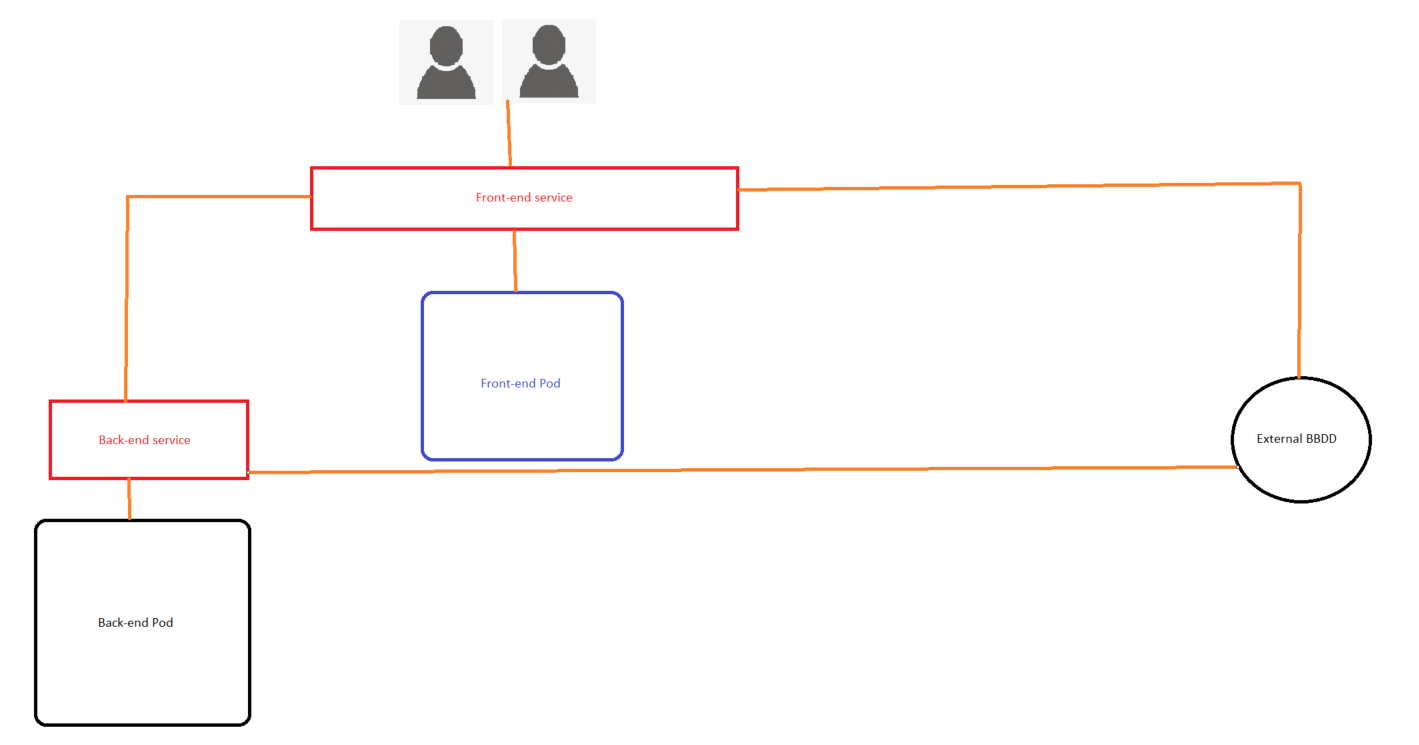
\includegraphics[width=\textwidth]{pictures/services.png}
\end{figure}

But in a higher level, how the users can access to applications running in Pods in a Woker Node?
We cannot access from outside the cluster to the Pod IP directly, because it is constantly changing and it just exists under K8s Network. Inside the cluster we can connect \verb|curl http://10.244.0.2|. But from outside? Now is when enters Service.

\begin{figure}[H]
    \centering
    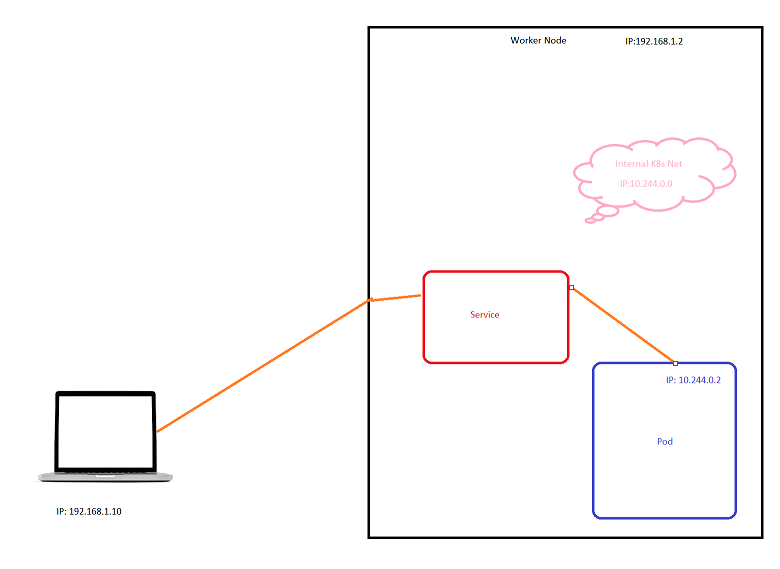
\includegraphics[width=\textwidth]{pictures/services2.png}
\end{figure}

\textbf{Service} is another K8s object like Pods, or ReplicaSets which forward requests to Pods.

There are three types of \textbf{Services:}
\begin{itemize}
    \item \textbf{Node Port Service:} it makes an internal port accesible on a port on the Node.
    \item \textbf{ClusterIP Service:} it creates a Virtual IP inside the cluster to enable communication between diferent applications (such as a set of front-end servers to a set of backend servers)
    \item \textbf{LoadBalancer:} it provides a Load Balancer to our application, for example to distribute the load across the different web servers in our front-end tier.
\end{itemize}

\subsubsection{NodePort Services}

\textbf{NodePort Services} listens on a port on the Node and forward requests on that port to a port on the Pod running the application. It makes a mapping of ports, mapping a port on the nodo to a port on the Pod. The Service is like a Virtual Server inside the Node. Inside the Cluster it has its own IP adress, called the ClusterIP of the Service.

There are 3 ports involved from the viewpoint of the Service:
\begin{itemize}
    \item \textbf{TargetPort:} Pod port where the app is running (80), that where the service forwars their request to.
    \item \textbf{Port:} Service port where the app is running (80)
    \item \textbf{NodePort:} Node port used to access the app externally (30008)
\end{itemize}

\begin{blocktemplateIII}{WARNING}
\textbf{NodePorts} can only be in a valid range which by default is from 30.000 to 32.767. As well, as Pods can run in any Node, \textbf{NodePort} are assigned to all the nodes at the same time, so we will be able to reach the application on each \textbf{Worker Node} on the \textbf{NodePort} assgined.
\end{blocktemplateIII}

\begin{figure}[H]
    \centering
    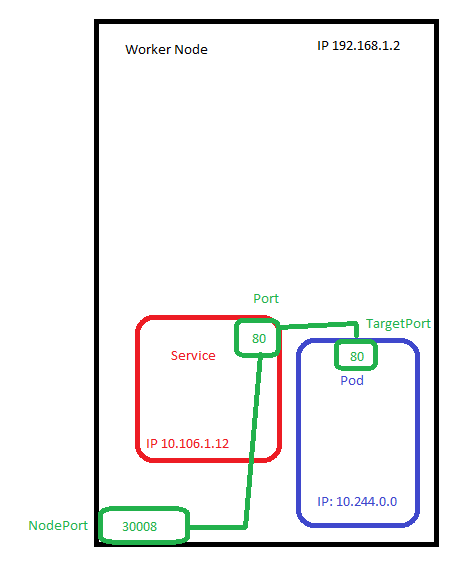
\includegraphics[scale=0.5]{pictures/services3.png}
\end{figure}

\subsubsection{How to define a NodePort Service?}

\begin{codetemplate}{service-template.yaml}
\begin{verbatim}
apiVersion: v1
kind: Service
metadata:
    name: myapp-service
    labels:
        tier: front-end
spec:
    type: NodePort
    selector:
        tier: front-end
    ports:
    - nodePort: 30008
      port: 80
      targetPort: 80
\end{verbatim}
\end{codetemplate}

As we discuss before, in the spec section we have only two fields:

\begin{itemize}
    \item\textbf{type:} NodePort, ClusterIP, LoadBalancer
    \item \textbf{ports:} list of port maps always agrouping (targetPort, Port and nodePort). we can have multiple such port mappings within a single service.
\end{itemize}

\begin{blocktemplateII}{NOTE}
If targetPort is not specified it is assumed to be the same as port, and if nodePort is not specified a free port on the Worker Node in the valid range between 30.000 and 32.767 is automatically assigned.
\end{blocktemplateII}

So, we have all the information in, but something is really missing. There is nothing in the definition file that connects the service to the Pod. We have simply specified the target port but we didn't mention the targetPort on which Pod. There could be hundreds of other Pods with applications running on port 80. So how do we do that?

As we did with the ReplicaSet, it is used a technique that we will see very often in K8s, \textbf{labels and selectors!} Selectors and labels are used to to link Services with Pods. But now \textbf{without matchLabels}

\subsubsection{How to create a Service using kubectl?}
\begin{codetemplate}{}
\begin{verbatim}
$ kubectl create -f service-template.yaml
\end{verbatim}
\end{codetemplate}

\begin{codetemplate}{}
\begin{verbatim}
$ kubectl get svc
\end{verbatim}
\end{codetemplate}

\begin{table}[H]
\begin{tabular}{| m{3cm} | m{2cm} | m{2.5cm} | m{2.7cm} | m{2cm} | m{1.2cm} |}
\hline
\textbf{NAME} & \textbf{TYPE} & \textbf{CLUSTER-IP} & \textbf{EXTERNAL-IP} & \textbf{PORT(S)} & \textbf{AGE} \\ \hline
myapp-service & NodePort & 10.106.127.123 & \verb|<none>| & 80:30008 & 5m \\ \hline
\end{tabular}
\end{table}

\textbf{PORT(S):} 80:30008/TCP

\textbf{PORT(S):} port:nodePort/TCP

You can access to the application from a terminal connecting with the \textbf{Worker Node IP} and \textbf{port}, because the Server will be listening on it.

\begin{codetemplate}{}
\begin{verbatim}
$ curl 192.168.1.2:30008
\end{verbatim}
\end{codetemplate}

\subsubsection{One Service, multiple instance of the same Pod}

So far, we have talked about a service mapped to a single Pod, but that's not the case all time. What do we do when we have multiple Pods? In a production environment it is common to have multiple instances of the same Pod, just to ensure High Availability if one replica fails and load balancing. In this case we have multiple Pods running our application, with all the same labels with a key-value app=myapp. This same label is created in the \textbf{.spec.selector} section during the creation of the Service.

So when the Service is created, it looks for a matching Pod with the labels specified in \textbf{.spec.selector}. The \textbf{Service} automatically selects all the Pods as endpoints to forward the external request.

\begin{blocktemplateI}{NOTE}
To load the balance between the instances, \textbf{Service} by default has the following configuration:

\begin{itemize}
    \item \textbf{Balance Policy:} Random
    \item \textbf{SessionAffinity:} yes
\end{itemize}
\end{blocktemplateI}

But what happens when the Pods are distributed across multiple Nodes (common case). In this case when we create a service, without us having to do any additional configuration (than labels), K8s automatically creates a Service that spans across all the Nodes in the cluster and maps the target port to the same Node port on all the Nodes in the Cluster.

\begin{figure}[H]
    \centering
    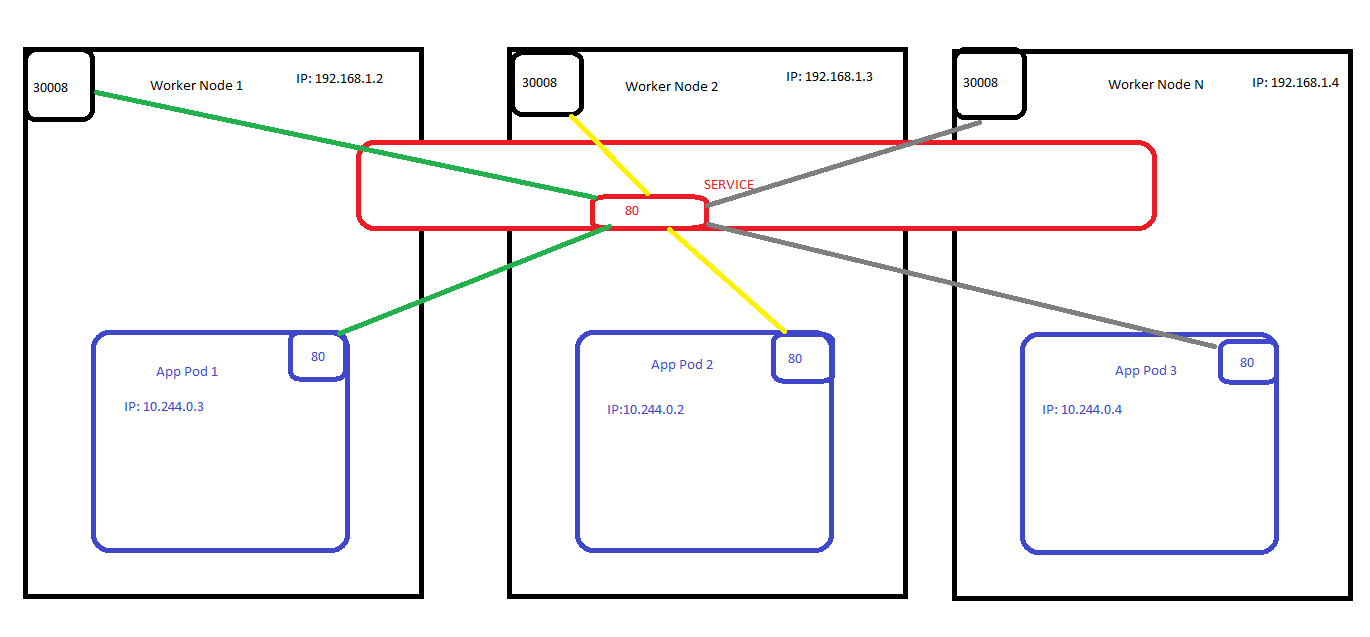
\includegraphics[width=\textwidth]{pictures/service5.png}
\end{figure}

This way, we can access our application using the IP of any Node in the cluster and using the same port number:

\begin{codetemplate}{}
\begin{verbatim}
$ curl 192.168.1.2:30004
\end{verbatim}
\end{codetemplate}

\begin{codetemplate}{}
\begin{verbatim}
$ curl 192.168.1.3:30004
\end{verbatim}
\end{codetemplate}

\begin{codetemplate}{}
\begin{verbatim}
$ curl 192.168.1.4:30004
\end{verbatim}
\end{codetemplate}

To summarize, in any case: whether it be a single Pod on a single Node, or multiple Pods on a single Node, or multiple Pods on Multiple Nodes. \textbf{The Service is created exactly the same} without we having to do any additional steps during the Service creation. \textbf{When Pods are removed or added with the correct labels the Service is automatically updated} making it highly flexible and adaptive. Once created, we don't have to make any additional configuration changes.

\subsubsection{Service ClusterIP}

Fullstack applications usually have different kinds of pods hosting different parts of an application. 
You may have a set of Pod instances of front-end a set of Pod instances of back-end and
a set of Pod instances of for example redis (key-value store) and another 
set of pods running for example a persistent DB like MySQL. 
Front-end servers needs to communicate with the back-end servers, 
and to the database and also to redis service, etc. So what is the best way to stabish the connection between these services or tiers of my application? 

Pods all have an IP adress assigned to them, but these IPs, as we know, are not static, these Pods can go down anytime and new Pods are created all the time, 
so we cannot rely on these IP adresses for internal communication between the application.

\textbf{ClusterIP Services} allow different applications or microservices of applications connect to each other inside the cluster using a \textbf{virtual IP}, which just exist inside the Cluster Network. 
This service create a kind of interface to group all the Pods of a microservice 
into a single IP reachable from other resources inside the cluster. 
In our example, the front-end Service work as unique interface to connect with front-end, same with backend, and same with redis. This enables us to easily and effectively deploy a microservice based application on K8s Cluster. \textbf{Every layer can now scale or move as required without impacting communication}.

A ClusterIP service is the \textbf{default service type in Kubernetes}, 
and it exposes the service \textbf{only within the cluster}. 
It assigns a virtual IP (known as the ClusterIP) that is \textbf{accessible from within the cluster pods and other services}.

The ClusterIP service is only accessible inside the cluster (i.e., from within the pods or other nodes that are part of the cluster network). The \textbf{worker node itself is not part of the Kubernetes pod network}, and its traffic is not routed from the worker nodes directly, only from within the pods or other Kubernetes-managed processes.

\begin{blocktemplate}{NOTE}
As well as have the ClusterIP, from inside the Pods, the best way to access the service is using the FQDN:
\begin{codetemplate}{}
\begin{verbatim}
service_name # If the pod is inside same namespace
\end{verbatim}
\end{codetemplate}
\begin{codetemplate}{}
\begin{verbatim}
service_name.namespace_name
\end{verbatim}
\end{codetemplate}
\end{blocktemplate}

\subsubsection{How to define a ClusterIP Service?}

\begin{codetemplate}{cluster-ip-service.yaml}
\begin{verbatim}
apiVersion: v1
kind: Service
metadata:
    name: front-end
    labels:
        name: myapp
spec:
    type: ClusterIP
    ports:
    - port: 80
      targetPort: 80
\end{verbatim}
\end{codetemplate}

As in the \textbf{NodePort} type:
\begin{itemize}
    \item \textbf{targetPort:} port exposed by the Pod
    \item \textbf{port:} port exposed by the service
    \item \textbf{selector:} to link the service to a set of Pods, copying the labels from the front-end Pod definition.
\end{itemize}

\begin{blocktemplateI}{NOTE}
The default Service type is \textbf{ClusterIP} so if we do not define Service type, by default it would be \textbf{ClusterIP}
\end{blocktemplateI}

\begin{codetemplate}{}
\begin{verbatim}
$ kc get svc
\end{verbatim}
\end{codetemplate}

\begin{table}[H]
\begin{tabular}{| m{3cm} | m{2cm} | m{2.5cm} | m{2.7cm} | m{2cm} | m{1.2cm} |}
\hline
\textbf{NAME} & \textbf{TYPE} & \textbf{CLUSTER-IP} & \textbf{EXTERNAL-IP} & \textbf{PORT(S)} & \textbf{AGE} \\ \hline
front-end & ClusterIP & 10.106.127.123 & \verb|<none>| & 80:30008 & 5m \\ \hline
\end{tabular}
\end{table}

\begin{figure}[H]
    \centering
    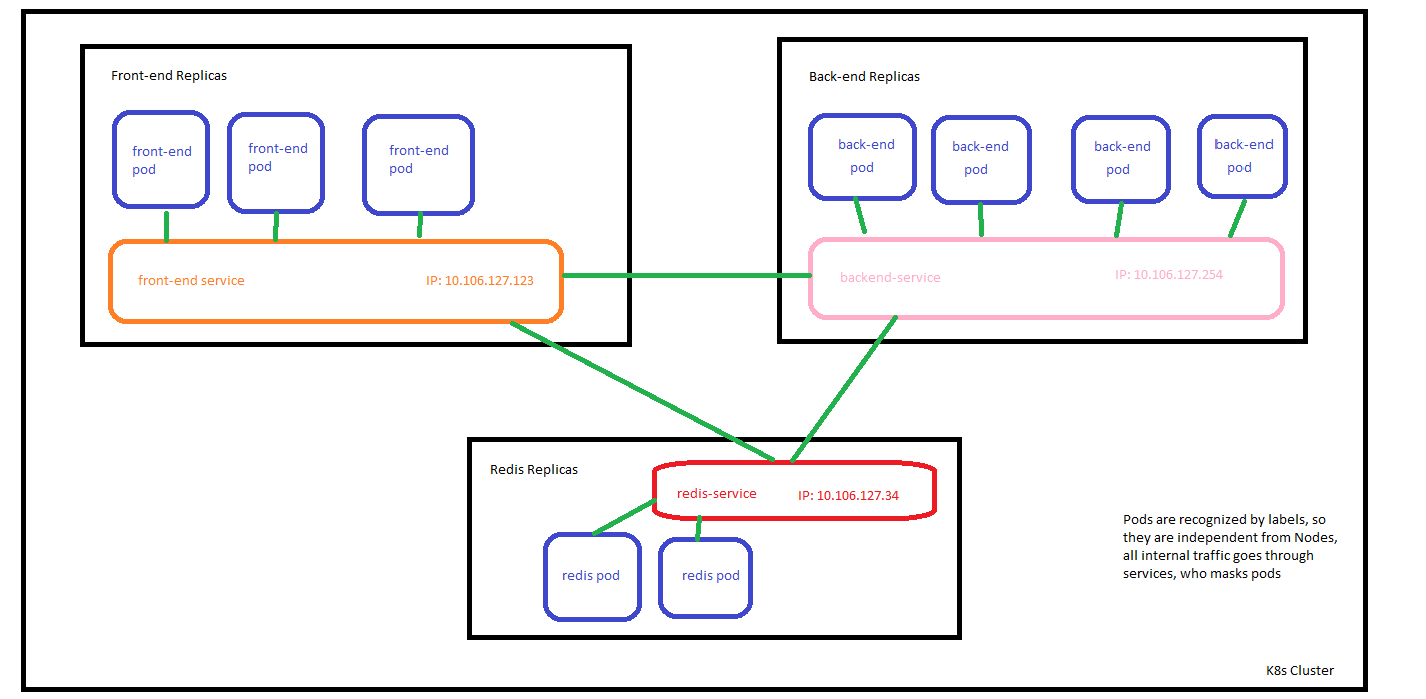
\includegraphics[width=\textwidth]{pictures/services4.png}
\end{figure}

\subsubsection{Service LoadBalancer}

Imagine the case of a web application to vote and see results, we have both services with their associated Pods with the apps running. There are many replicas of each Pod running on different Nodes, and the Service is a NodePort service. As we know a NodePort services expose the app in a specific port of the Worker Nodes, so... What URL users should use to access the voting web, or the result web? They can use 4 IP's with its port to vote and 4 IP's with its port for the results. This is not what users want, they want single urls (like www.results.com).

So, \textbf{LoadBalancer Service} create a new VM for load balancer configuring in this VM a suitable load balancer as HAProxy or NGINX. Then configure the Load Balancers (as NGINX) to route traffic to the underlying Nodes and expose a single endpoint.

If we are on a Supported Cloud Platform as Google, AWS, Azure... It could leverage the native load balancer off that cloud platform. K8s has support for integrating with the native load balancers of certain cloud providers, configuring that for us. So all we need to do is setup our service type as LoadBalancer, letting the rest as NodePort service.

\begin{figure}[H]
    \centering
    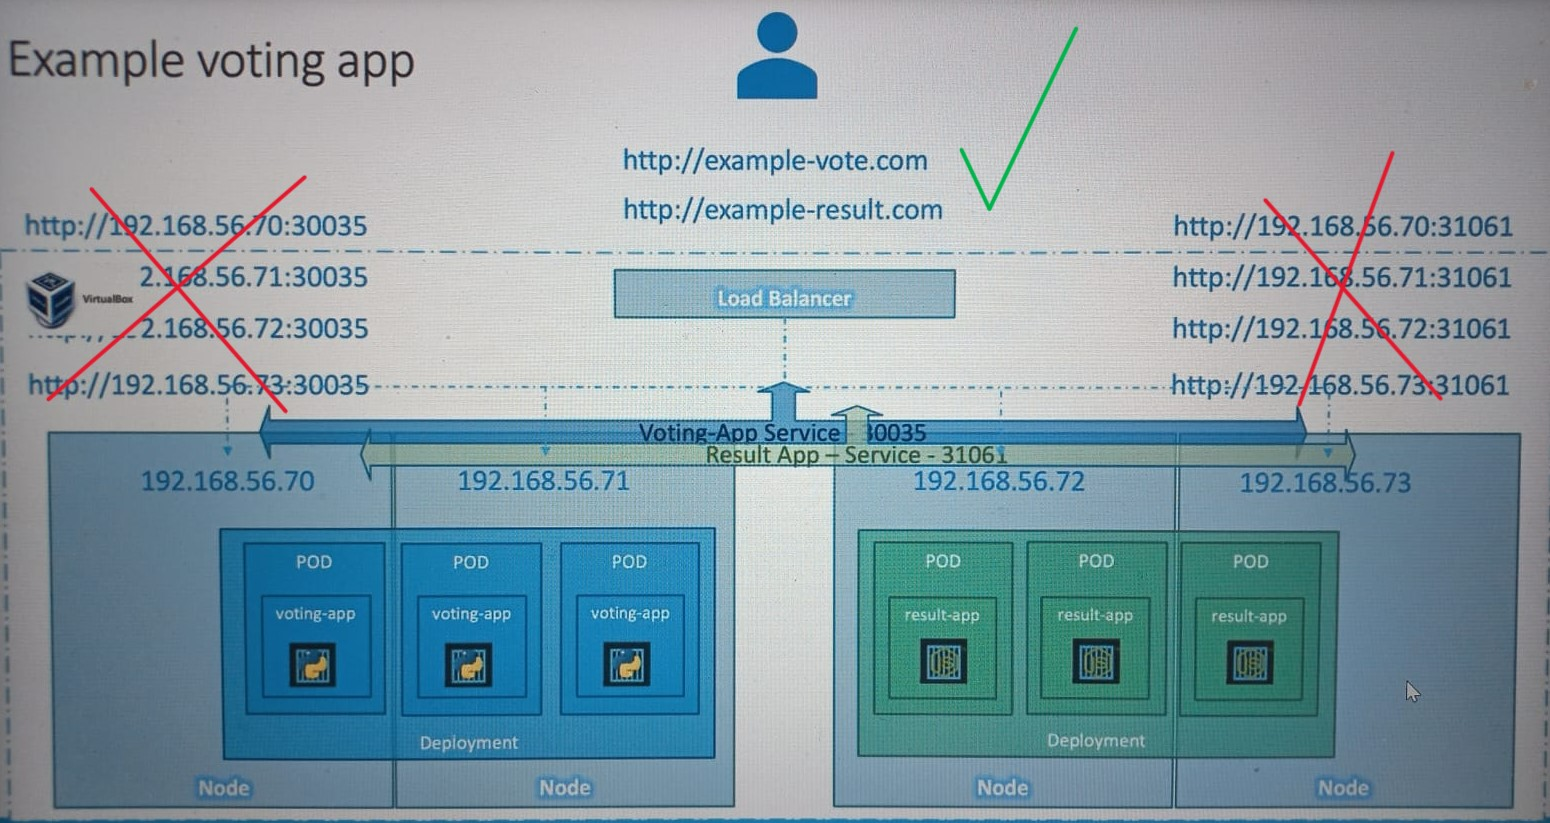
\includegraphics[width=\textwidth]{pictures/services5.jpeg}
\end{figure}

\subsubsection{How to define a NodeBalancer Service?}

\begin{codetemplate}{node-balancer-service.yaml}
\begin{verbatim}
apiVersion: v1
kind: Service
metadata:
    name: nginx-service
    labels:
        name: nginx
spec:
    type: LoadBalancer
    ports:
    - nodePort: 30008
      port: 80
      targetPort: 80
\end{verbatim}
\end{codetemplate}

\begin{blocktemplateIII}{WARNING}
LoadBalancer Services only work with Supported Cloud Platforms, as Azure, AWS, Google Cloud...    
\end{blocktemplateIII}

\subsubsection{K8s DNS: How to reach the services from other Pods?}
To reach a ClusterIP service from other pods within the same Kubernetes cluster, we can use the service's DNS name or its ClusterIP address. The Kubernetes service discovery and networking setup make it easy for pods to communicate with each other using these methods.

Kubernetes automatically sets up DNS serever within the cluster (as pods in kube-system namespace). Each service gets a DNS name based on its name and the namespace it is running in. DNS Name Format: 
\begin{codetemplate}{}
\begin{verbatim}
<service-name>.<namespace>.svc.cluster.local
\end{verbatim}
\end{codetemplate}

Kubernetes will automatically resolve this DNS name to the ClusterIP and route the traffic to the service, which in turn forwards it to the appropriate pod.

\begin{blocktemplateII}{NOTE}
If the pod accessing the service is in the same namespace, we can use the \verb|service_name| directly:
\begin{codetemplate}{}
\begin{verbatim}
$ curl <service_name>:<service_port>
\end{verbatim}
\end{codetemplate}
\end{blocktemplateII}

You can also reach the service by directly using its ClusterIP. However, this requires knowing the IP address assigned to the service and it is not a best practice. It's better to rely on DNS instead of the IP address, as the IP can change if the service is deleted and recreated, whereas the DNS name is stable.
\begin{codetemplate}{}
\begin{verbatim}
$ curl <service_clusterIP>:<service_port>
\end{verbatim}
\end{codetemplate}

\subsubsection{CurlPod: How to reach the services from the Nodes?}
If the Service is \textbf{NodePort} type, we will be able to reach it directly by:
\begin{codetemplate}{}
\begin{verbatim}
$ curl localhost:<service_port>
\end{verbatim}
\end{codetemplate}

If there is of another type, we will be able to reach it:
\begin{codetemplate}{}
\begin{verbatim}
$ curl <service_IP>:<service_port>
\end{verbatim}
\end{codetemplate}

But, as we will see in future sections, the dns resolution is configured just at Pod level, so only from within the pods we will be able to reach
the services or other pods using their different \textbf{FQDNs}.

The best approach then will be to run a \textbf{Pod} inside the namespace of the \textbf{Service} and use the curl tool:

\begin{codetemplate}{}
\begin{verbatim}
$ kubectl run curlpod --image=alpine/curl -it --rm --restart=Never \
    --command -- curl http://<service_name>:<service_port>
\end{verbatim}
\end{codetemplate}

\subsubsection{Port Forward: How to reach the services from outside the cluster}
\paragraph{Introduction}
Port-forwarding in Kubernetes (K8s) is a mechanism that allows we to access a specific resource (like a service or a pod) inside a Kubernetes cluster from our local machine. Typically, resources inside the cluster are isolated, and they can't be directly accessed from outside the cluster. However, by using port-forwarding, we can temporarily expose a local port to connect to a port of a service or a pod inside the cluster, which is especially useful for debugging, testing, or accessing internal applications.

Port-forwarding works by forwarding traffic from a local port on our machine to a port on a resource (like a service or pod) inside the Kubernetes cluster. This allows we to communicate with applications running inside the cluster without needing to expose them externally.

\paragraph{Use Cases}
\begin{itemize}
    \item \textbf{Access} internal services (e.g., databases or web services) without exposing them externally.
    \item \textbf{Debug} and \textbf{test} applications by directly accessing their endpoints.
    \item For local development, interact with in-cluster resources as if they were running locally.
\end{itemize}

\paragraph{kubectl port-forward}
Services in Kubernetes manage access to a group of pods. By port-forwarding to a service, we can reach any pod behind the service (whichever the service forwards traffic to). Here's how to port-forward a service to our local machine.

\begin{codetemplate}{}
\begin{verbatim}
$ kubectl port-forward service <service_name> <local_port>:<service_port>
\end{verbatim}
\end{codetemplate}

Sometimes, we may want to port-forward directly to a specific pod. This can be useful if we want to directly access an individual pod (not through a service), or if you're testing or debugging a particular instance of our application.
\begin{codetemplate}{}
\begin{verbatim}
$ kubectl port-forward pod <pod_name> <local_port>:<image_port>
\end{verbatim}
\end{codetemplate}

%=====================================================
\newpage
\subsection{Namespaces}

\href{https://kubernetes.io/docs/concepts/overview/working-with-objects/namespaces/}{Official K8s Doc}

\subsubsection{Introduction to Namespaces}
\label{IntNames}

Let's start this section with an analogy. There are 2 boys called Mark, as they have the same name, people in general call them for their last name. But, in his houses, his family call them for their names, but out of the house, they should be called by the full-name (name and last name). In this analogy, houses are namespaces.

\begin{figure}[H]
    \centering
    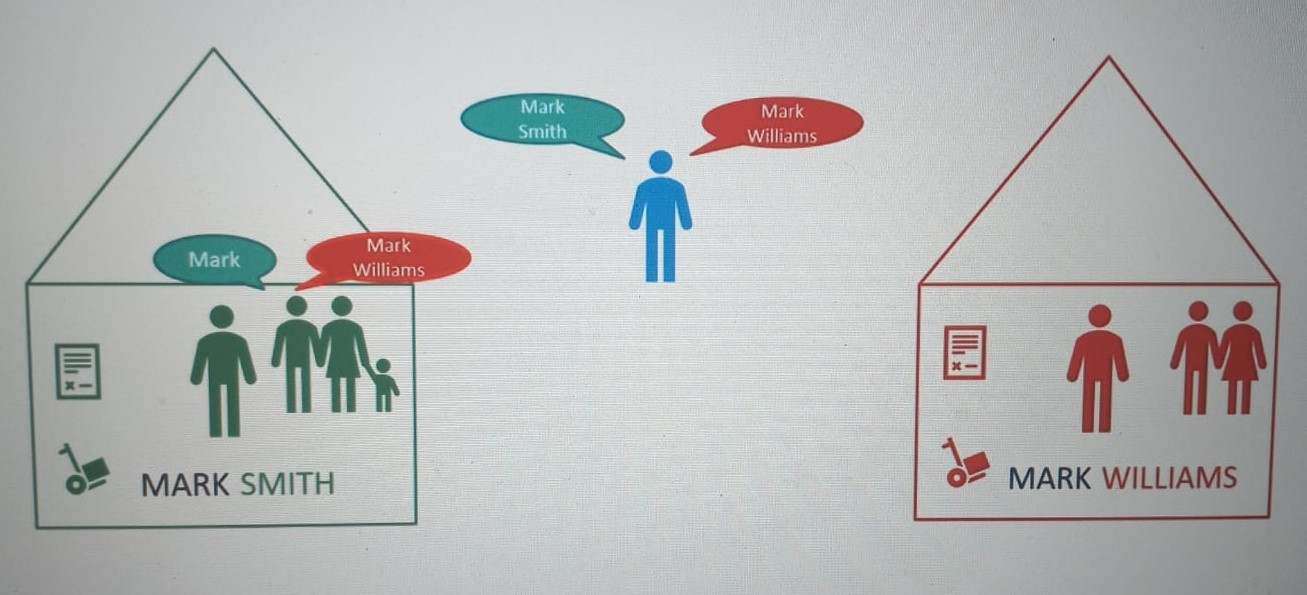
\includegraphics[scale=0.4]{pictures/namespace1.jpeg}
\end{figure}

So, K8s resources within a \textbf{Namespace} can refer to each other simply by their names. In the following example the web app Pod can reach the db-service simply using the hostname db-service. 

\begin{figure}[H]
    \centering
    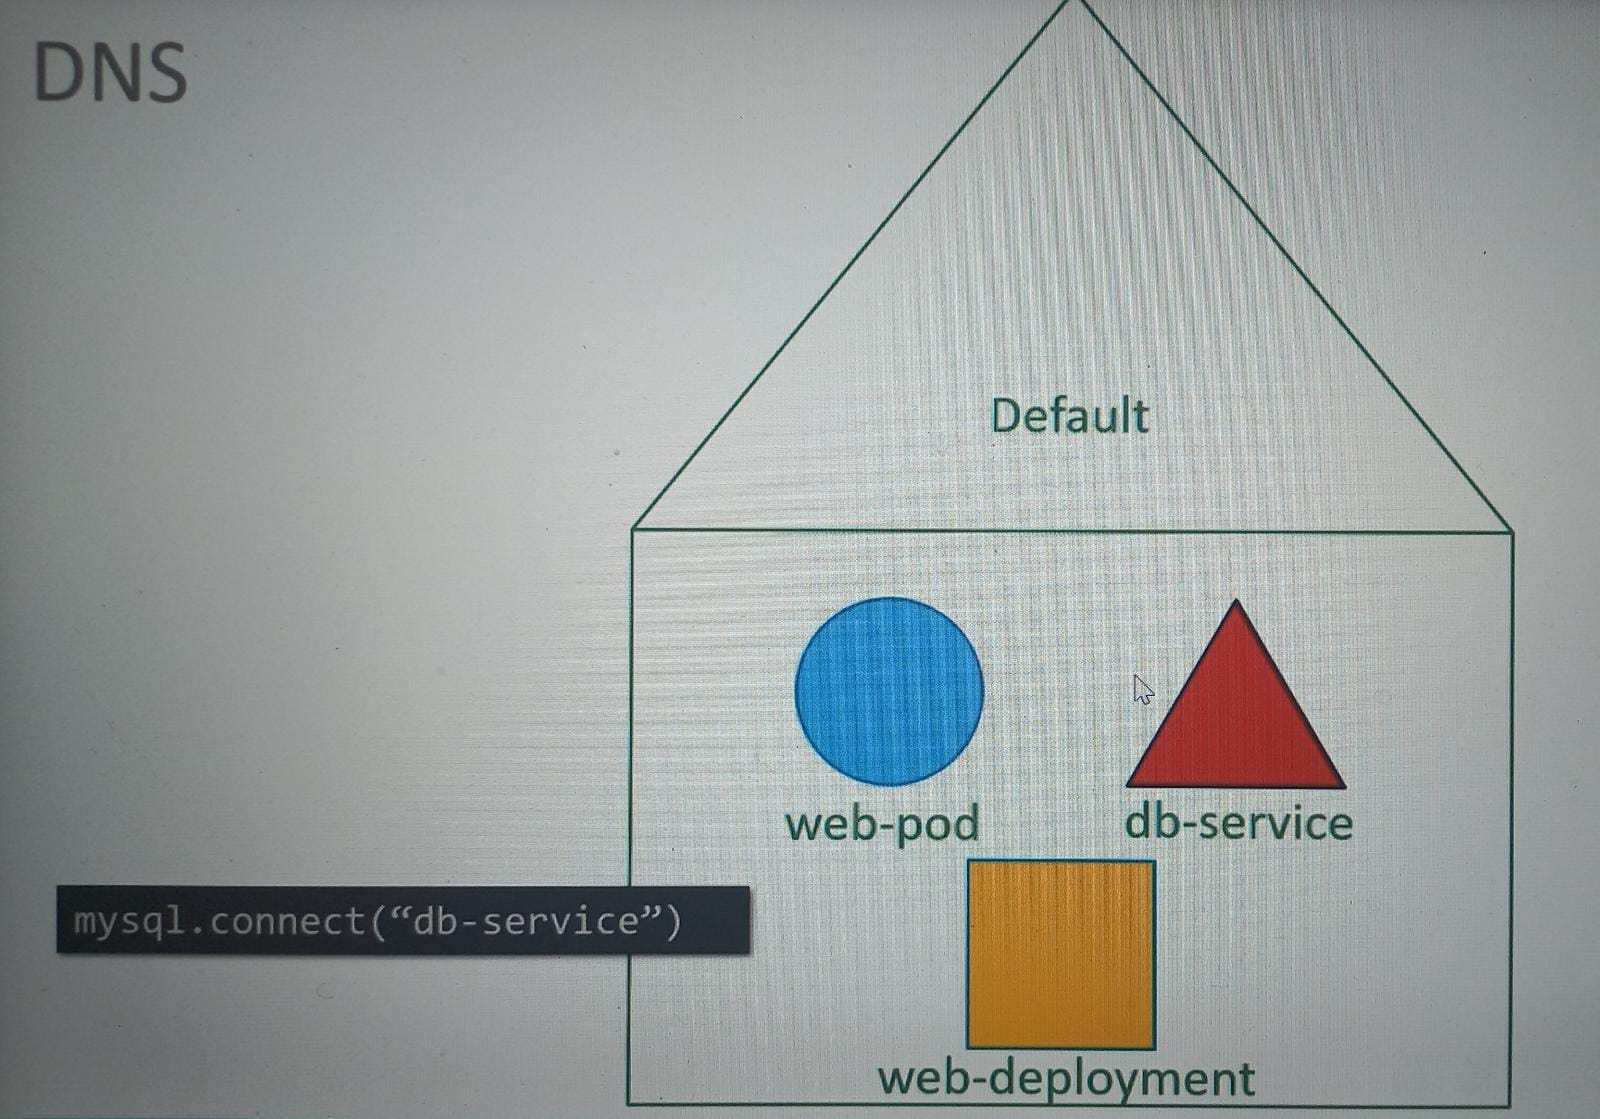
\includegraphics[scale=0.2]{pictures/namespace2.jpeg}
\end{figure}

If required, the web app pod can reach a service in another Namespace as well, but for this, we must \textbf{append the name of the Namespace to the name of the service}. Using the format:

\begin{codetemplate}{}
\begin{verbatim}
servicename.namespace.svc.cluster.local
\end{verbatim}
\end{codetemplate}

\begin{figure}[H]
    \centering
    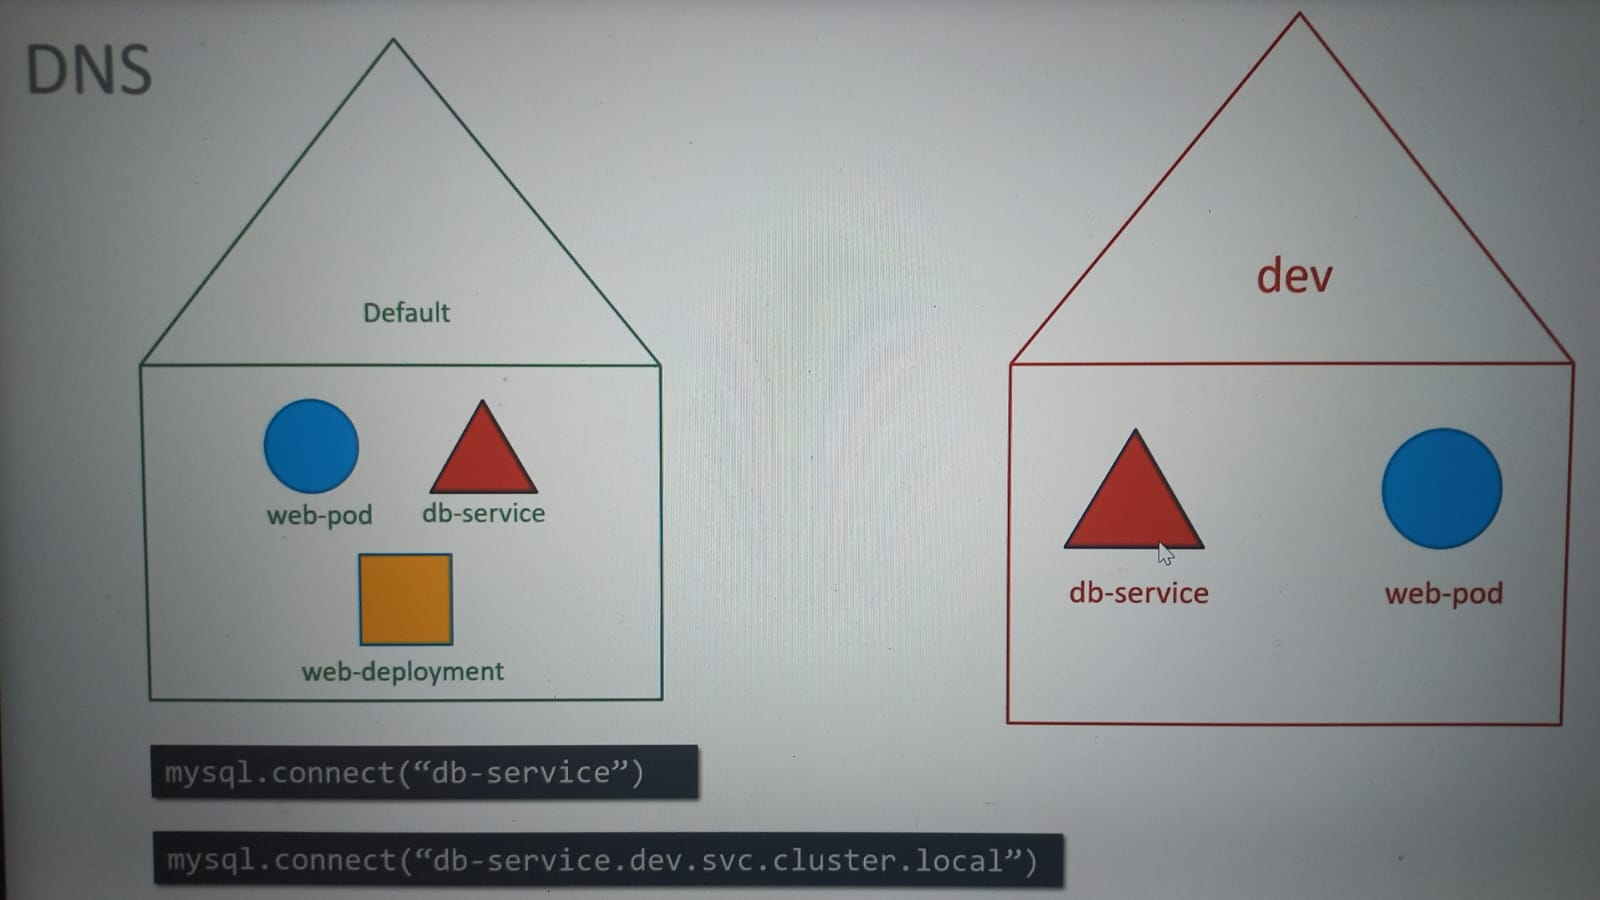
\includegraphics[scale=0.22]{pictures/namespace3.jpeg}
\end{figure}

You can use this format because when a Service is created, a DNS entry is added automatically in this format. Looking closely at the DNS name of the service:
\begin{itemize}
    \item \textbf{.cluster.local:} default domain name of the K8s cluster
    \item \textbf{.svc:} sub domain for service
    \item \textbf{.dev:} sub domain for namespace
    \item \textbf{db-service:} sub domain for the object named itself
\end{itemize}

\begin{figure}[H]
    \centering
    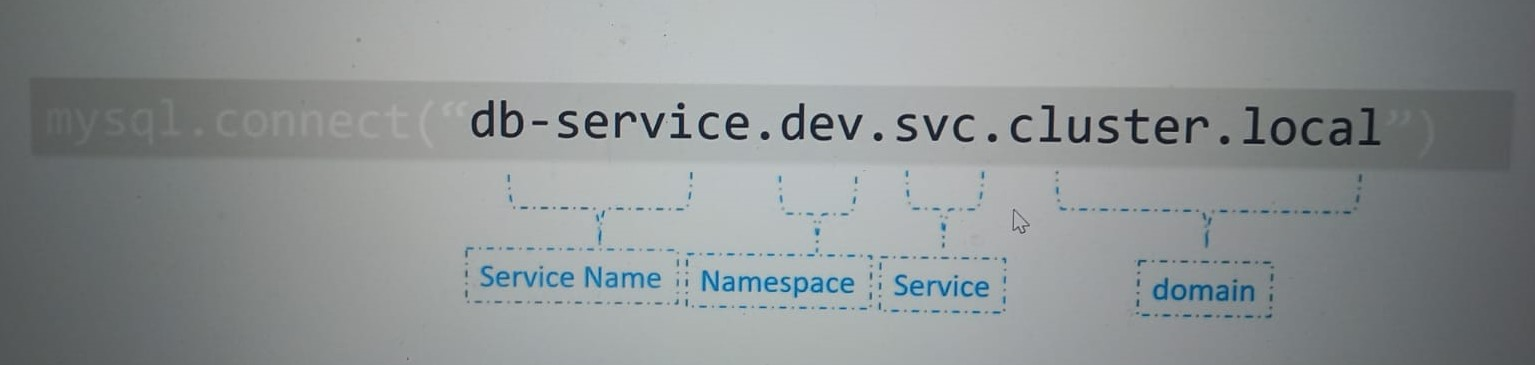
\includegraphics[scale=0.3]{pictures/namespace4.jpeg}
\end{figure}

\subsubsection{K8s automatically created Namespaces}

So far, all the creation we have been done in K8s with kubectl has been done in a house. Yes! We have been deceived. This \textbf{Namespace} is \textbf{Default}. and it is created automatically by K8s when the cluster is first setup. 

K8s creates a set of Pods and Services for its internal purpose, such as those required by the Networking solution, DNS Server, etc. To isolate them from the user and to prevent accident deletions or modifications of these objects K8s creates them under another \textbf{Namespace} created at Cluster startup named \textbf{kube-system}.

A third \textbf{Namespace} created by K8s automatically is called \textbf{kube-public}, this is where resources that should be made available to all users are created.

If our environment is small or we are playing arouund with a small cluster, we shouldn't really have to worry about \textbf{Namespaces}. we can continue working in the \textbf{default} \textbf{Namespace}. However, as in when we grow and use a K8s cluster for enterprise or production purposes, we may want to consider the use of \textbf{Namespaces}.

\subsubsection{Create own Namespaces}

Imagine that we want to isolate dev environment resources from production resources, we can create a different Namespace for each of them. That way, if we are working in the dev environment, we dont accident modify production objects.

\paragraph{Difficult way to create a Namespace}

Like any other object in K8s, it is necessary to use a \textbf{Namespace} definition file to create a new Namespace:

\begin{codetemplate}{namespace-template.yaml}
\begin{verbatim}
apiVersion: v1
kind: Namespace
metadata:
    name: test-namespace
\end{verbatim}
\end{codetemplate}

Now run the following command and we will have our new Namespace ready!

\begin{codetemplate}{}
\begin{verbatim}
$ kubectl create -f namespace-template.yaml
\end{verbatim}
\end{codetemplate}

\paragraph{Easy way to create a Namespace}

\begin{codetemplate}{}
\begin{verbatim}
$ kubectl create namespace tst-namespace
\end{verbatim}
\end{codetemplate}

\subsubsection{kubectl commands to manage Namespaces}

\textbf{Looking for resources}
\begin{codetemplate}{}
\begin{verbatim}
$ kubectl get po -n <namespace_name>
\end{verbatim}
\end{codetemplate}

\textbf{Get a resource for all namespaces}
\begin{codetemplate}{}
\begin{verbatim}
$ kubeclt get <resource> --all-namespaces [-A]
\end{verbatim}
\end{codetemplate}

\textbf{Creating resources}
\begin{codetemplate}{}
\begin{verbatim}
$ kubectl create -f pod-def.yaml -n <namespace_name>
\end{verbatim}
\end{codetemplate}

\textbf{See all namespaces in our K8s Cluster}
\begin{codetemplate}{}
\begin{verbatim}
$ kubectl get ns (namespaces)
\end{verbatim}
\end{codetemplate}

\begin{blocktemplateIII}{WARNING}
If we do not pass namespace tu kubectl commands, it would be set as the current namespace. If we do not switched it once entered the cluster, it is default
\end{blocktemplateIII}

\textbf{Switch the current Namespace}
\begin{codetemplate}{}
\begin{verbatim}
$ kubectl config set-context --current --namespace <desired_namespace>
\end{verbatim}
\end{codetemplate}

\begin{blocktemplateI}{NOTE}
Context are used to manage multiple Clusters and multiple environments from the same management system. It is a totally separate topic to discuss and requires its own section.
\end{blocktemplateI}

\subsubsection{Defining Namespace in K8s Objects}

The definition of Namespace to create objects on it must be done in .metadata.namespace.

\underline{EXAMPLES:}

\begin{codetemplate}{pod-namespaced.yaml}
\begin{verbatim}
apiVersion: v1
kind: Pod
metadata:
    name: myapp
    namespace: dev
    labels:
        app: myapp
        tier: front-end
spec:
    containers:
    - ...
\end{verbatim}
\end{codetemplate}

\begin{codetemplate}{service-namespaced.yaml}
\begin{verbatim}
apiVersion: v1
kind: Service
metadata:
    name: myapp-service
    namespace: dev
spec:
    ports:
    - nodePort: 30080
      port: 8080
      protocol: TCP
      targetPort: 8080
    selector:
        app: myapp
        tier: front-end
    type: NodePort 
\end{verbatim}
\end{codetemplate}

\subsubsection{Namespace Policies}

\href{https://kubernetes.io/docs/concepts/policy/resource-quotas/}{Official K8s Doc}

\label{Quota}
Each Namespace can have its own set of policies that define who can do what. we can also assign quota of resources to each of these Namespaces (like we do in ICP). To limit resources in a Namespace, we should create a \textbf{Resource Quota}

\textbf{Define it}
\begin{codetemplate}{resource-quota.yaml}
\begin{verbatim}
apiVersion: v1
kind: ResourceQuota
metadata:
    name: compute-quota
    namespace: dev
spec:
    hard:
        pods: "10"
        requests.cpu: "4"
        requests.memory: 5Gi
        limits.cpu: "10"
        limits.memory: 10Gi
\end{verbatim}
\end{codetemplate}

This allows a maximum of 10 Pods, or 4 request CPU, or 5GI memory request...

\textbf{Create it in the namespace dev}
\begin{codetemplate}{}
\begin{verbatim}
kubectl create -f resource-quota.yaml -n dev
\end{verbatim}
\end{codetemplate}

\subsection{Imperative vs Declarative, apply command}

\subsubsection{Introduction}

As we have seen, there are different ways of creating and managing K8s Objects. We created objects directly by running commands as well as using object configuration files. In the \textbf{Infraestructure as a Code World}, there are different approaches in managing the infraestructure, classified into \textbf{Imperative} or \textbf{Declarative} approaches.

\textbf{Imperative} approaches are if we are co-pilot in a car and we say to the driver all the actions he must take, turn to the left, and no to the right, no straight, ecct. \textbf{Declarative} is to say, this is the final destination, and the driver figures out the path.

In \textbf{Imperative} approaches we say step by step what to do, and at what time. In \textbf{Declarative} we just make a list of requirements, and everything that's needed to be done to get this infraestructure in place is done by the system or the software. It is no necessary to provide step-by-step instructions. Orchestration tools like Nasible, Puppet, Chef or Terraform fall into this category.

\begin{figure}[H]
    \centering
    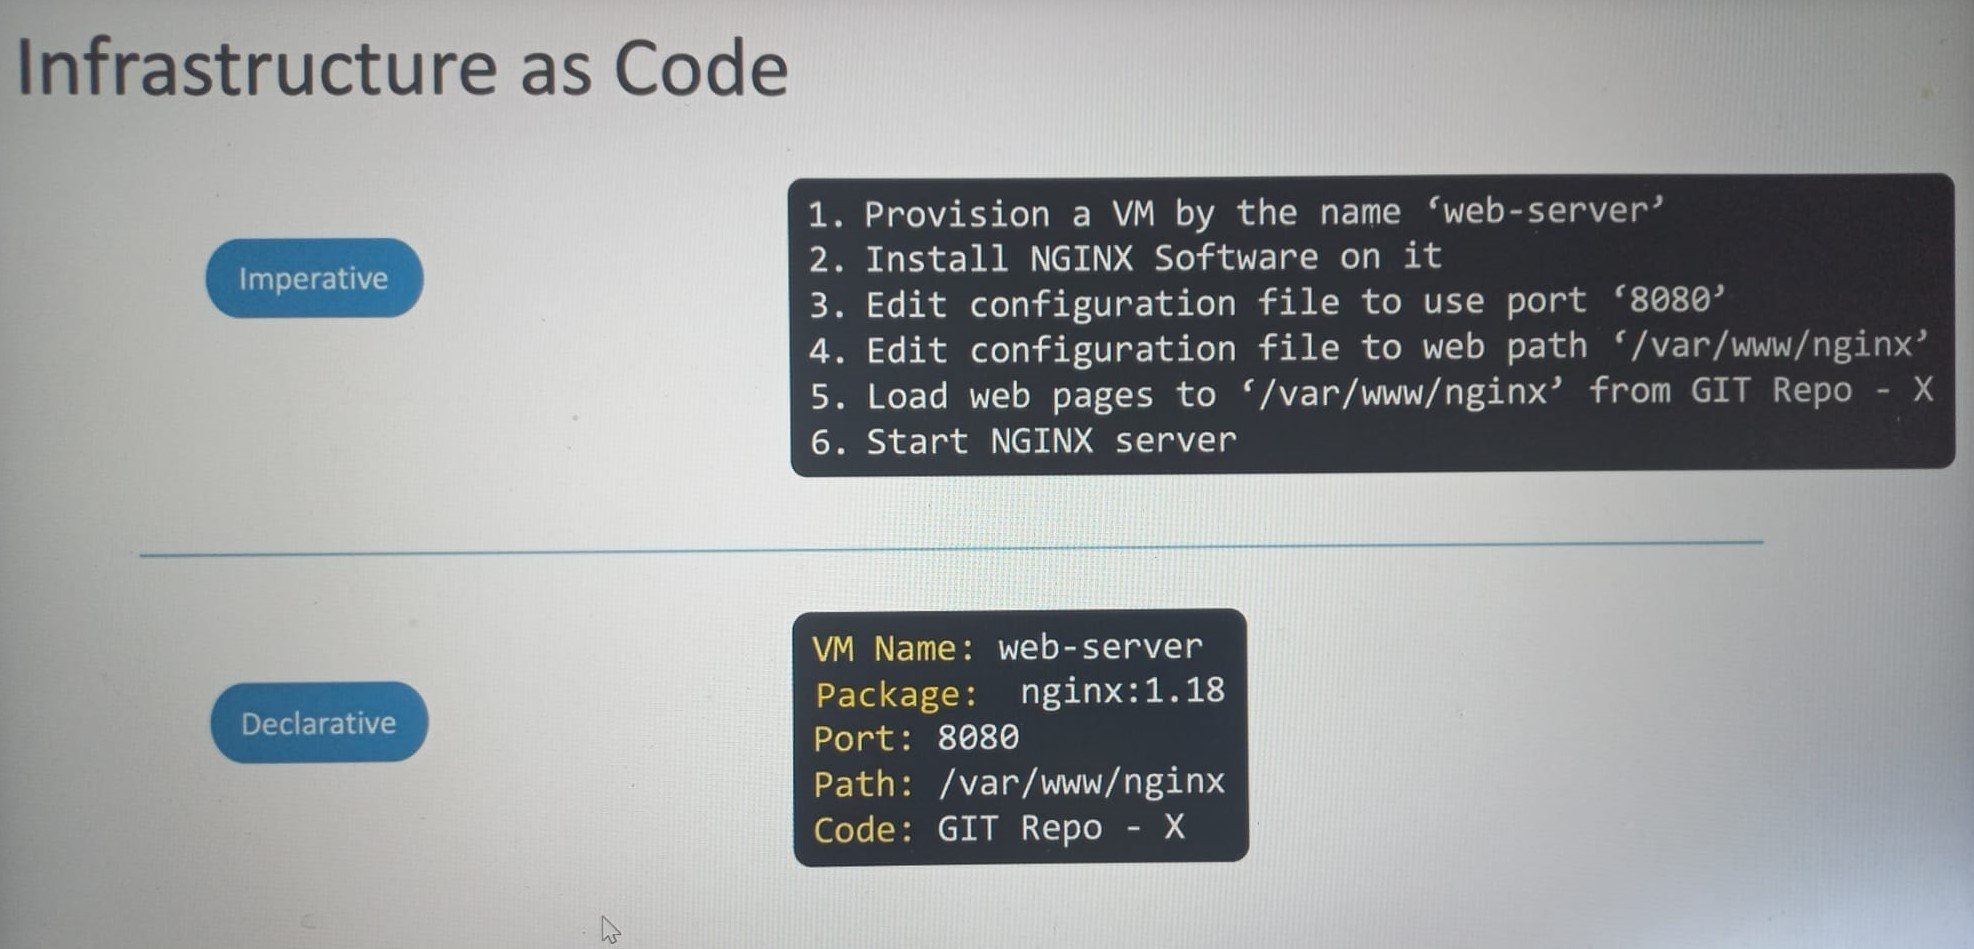
\includegraphics[width=\textwidth]{pictures/impdec.jpeg}
\end{figure}

What happen in imperative way if the VM is already instaled, if we want to change the configuration for port 8080, or if we want to upgrade the NGINX version. we have to add more steps to do such things. However,in a declarative way, is as simple as change the version, port or what we need in the declaration file, system should be intelligent enough what has already been done and apply the necessary changes only.

The way we have to run declarative instructions in K8s is with the \verb|kubectl apply| command, for creating, updatingm or deleting an object. The apply command will look at the existing configuration and figure out what changes neet to be made to the system.

\subsubsection{Working Imperative}

Imagine we have created a K8s Objetc:

\begin{codetemplate}{}
\begin{verbatim}
$ kubectl create -f deployment_template.yaml
\end{verbatim}
\end{codetemplate}

But now, once it is running, we want to modify something on it, for example the image of the Pod container because there is a new version available. So we can use the edit command and do it:

\begin{codetemplate}{}
\begin{verbatim}
$ kubectl edit deployment <object-name>
\end{verbatim}
\end{codetemplate}

When this command is run, an interactive terminal is open with a YAML definition file similar to the one we used to create the object but with some additional fields, such as the status fields, ect. \textbf{This is not the file we used to create the object, this is a similar Pod definition file within K8s memory}. If we make changes to this file, save and quit, those changes will be applied to the live object, but never to the definition object YAML file.

This is not a good way to work for production environments, so if in the future, a teammate decides to make a change to this object unaware that a change was made using the \verb|kubectl edit| command an deploys a new version the previous change is lost. So it is hardly recommended to use \verb|kubectl edit| only for tests or changes that we are not going to rely on the object configuration file in the future.

The best way to do it is always declarative:
\begin{codetemplate}{}
\begin{verbatim}
$ kubectl get deploy <deployment_name> -o yaml > deployment_template.yaml
\end{verbatim}
\end{codetemplate}
\begin{codetemplate}{}
\begin{verbatim}
$ vim deployment_template.yaml
\end{verbatim}
\end{codetemplate}
\begin{codetemplate}{}
\begin{verbatim}
$ kubectl apply -f deployment_template.yaml
\end{verbatim}
\end{codetemplate}

\begin{blocktemplateII}{NOTE}
There is a way to record changes in both file and object in an imperative way, because we say directly to K8s to replace the object:
\begin{codetemplate}{}
\begin{verbatim}
$ kubectl replace -f deployment_template.yaml
\end{verbatim}
\end{codetemplate}
If the replace command finds that the object we want to replace does not exist it fails. Like if we run the \verb|kubectl create| command and the object already exists, it will fail.
\end{blocktemplateII}

\begin{blocktemplateIII}{WARNING}
You need to pay attention on \verb|kubectl edit| command, because it is very easy to fail, as there are a lot of fields which are \textbf{unmutable}. In case of failure we hardly recommend:
\begin{itemize}
    \item Follow the procedure of:
\begin{codetemplate}{}
\begin{verbatim}
$ kubectl get deploy <deployment_name> -o yaml > deployment_template.yaml
\end{verbatim}
\end{codetemplate}
\begin{codetemplate}{}
\begin{verbatim}
$ vim deployment_template.yaml
\end{verbatim}
\end{codetemplate}
\begin{codetemplate}{}
\begin{verbatim}
$ kubectl apply -f deployment_template.yaml
\end{verbatim}
\end{codetemplate}

    \item If the error persists, then replace the hardway:
\begin{codetemplate}{}
\begin{verbatim}
$ kubectl replace -f deployment_template.yaml --force
\end{verbatim}
\end{codetemplate}
\end{itemize}
\end{blocktemplateIII}

\subsubsection{Working Declarative}

First, edit the Object declaration YAML file:
\begin{codetemplate}{}
\begin{verbatim}
$ vim deployment-template.yaml
\end{verbatim}
\end{codetemplate}

Once we have made the required changes, we apply them:
\begin{codetemplate}{}
\begin{verbatim}
$ kubectl apply -f deployment-template.yaml
\end{verbatim}
\end{codetemplate}

This way, going forward, the changes made are recorded and can be tracked as part of the change review process. The \verb|kubectl apply| command is intelligent enough to create an object if it doesn't already exist.

If we pass a path as argument it will create or modify all objects related to the YAML files inside the path.

\begin{codetemplate}{}
\begin{verbatim}
$ kubectl apply -f /path/to/yamls/
\end{verbatim}
\end{codetemplate}

For more information
\begin{codetemplate}{}
\begin{verbatim}
$ kubectl apply --help
\end{verbatim}
\end{codetemplate}

\subsubsection{kubectl apply}

\href{https://jamesdefabia.github.io/docs/user-guide/kubectl/kubectl_apply/}{Official K8s Doc}

It takes into consideration local configuration file or files to update, create, remove or do some task with K8s Objects. It compares the file and the last applied configuration before making a decision on what changes are to be made.

Also, when we use \verb|kubectl apply| command our local YAML object configuration file is converted to a JSON format an it is then stored as the last applied configuration. Going forward, for any updates to the object, all the three files are compared to identify what changes are to be made on the live object. This new JSON file is stored on the live object configuration YAML file itself, as an annotation named last applied configuration. But it is only done when we use the apply command.

\begin{figure}[H]
    \centering
    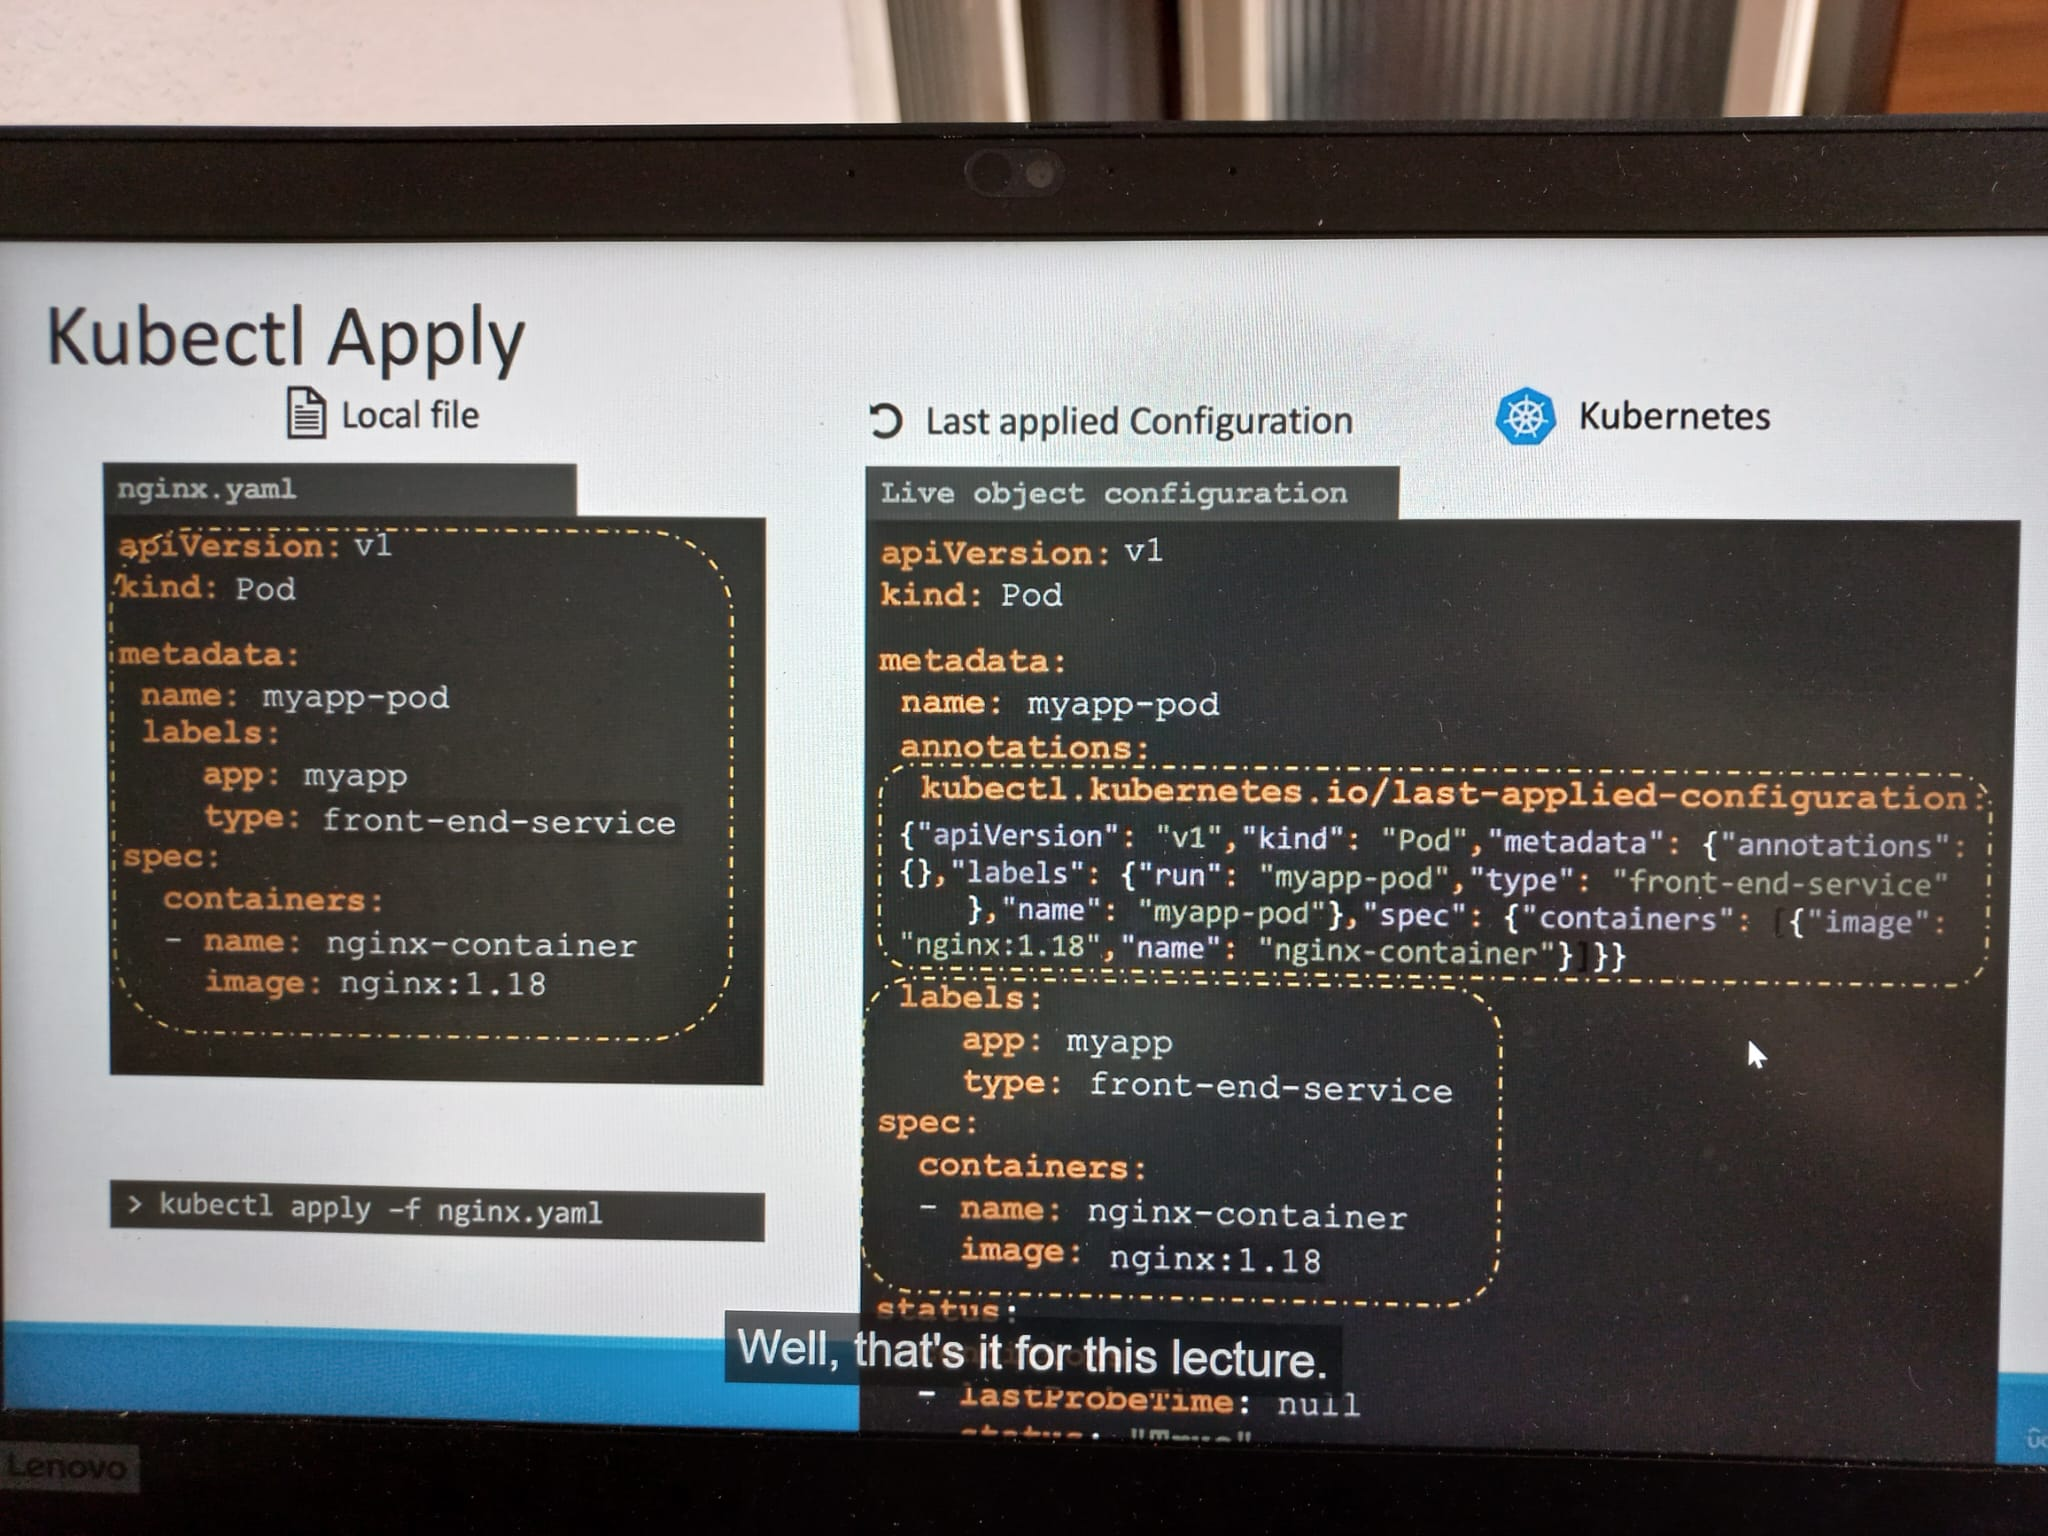
\includegraphics[width=\textwidth]{pictures/apply1.jpeg}
\end{figure}

%======================================================
\newpage
\section{Labels, Selector \& Annotations}

\href{https://kubernetes.io/docs/concepts/overview/working-with-objects/labels/}{Official K8s Doc}

\subsection{Introduction}

\textbf{Labes \& Selectors} are K8s standard method to group thnigs together. Imagine we have a lot of annimals of different species and the K8s Objects and Users want to be able  to filter them based on different criteria: 

\begin{itemize}
    \item Based on their type: mammals, fish, reptiles, birds, arthropods, amphibians...
    \item Based on if they life in the watter or not
    \item Based on their climatic region
    \item Based on their feeding: omnivores, vegetarian, carnivore, scavenger...
\end{itemize}

We can use any classification we want, the point is we use them to filter a set of Objects based on a defined criteria.

So in K8s, it is a very best practice to define Labels anywhere, so in the future we can filter and find the objects desired in every situation.

So in a K8s cluster, we will have hundreds of thousands K8s Objects, Pods, Deployments, ReplicaSets, Services, Ingress, PV's, ConfigMaps... And we will need to filter and to group all this Objects in different sets, for example to determine all the objects involved in an app, or by their functionality, we never know when we will need to filter.

Filtering by app:

\begin{figure}[H]
    \centering
    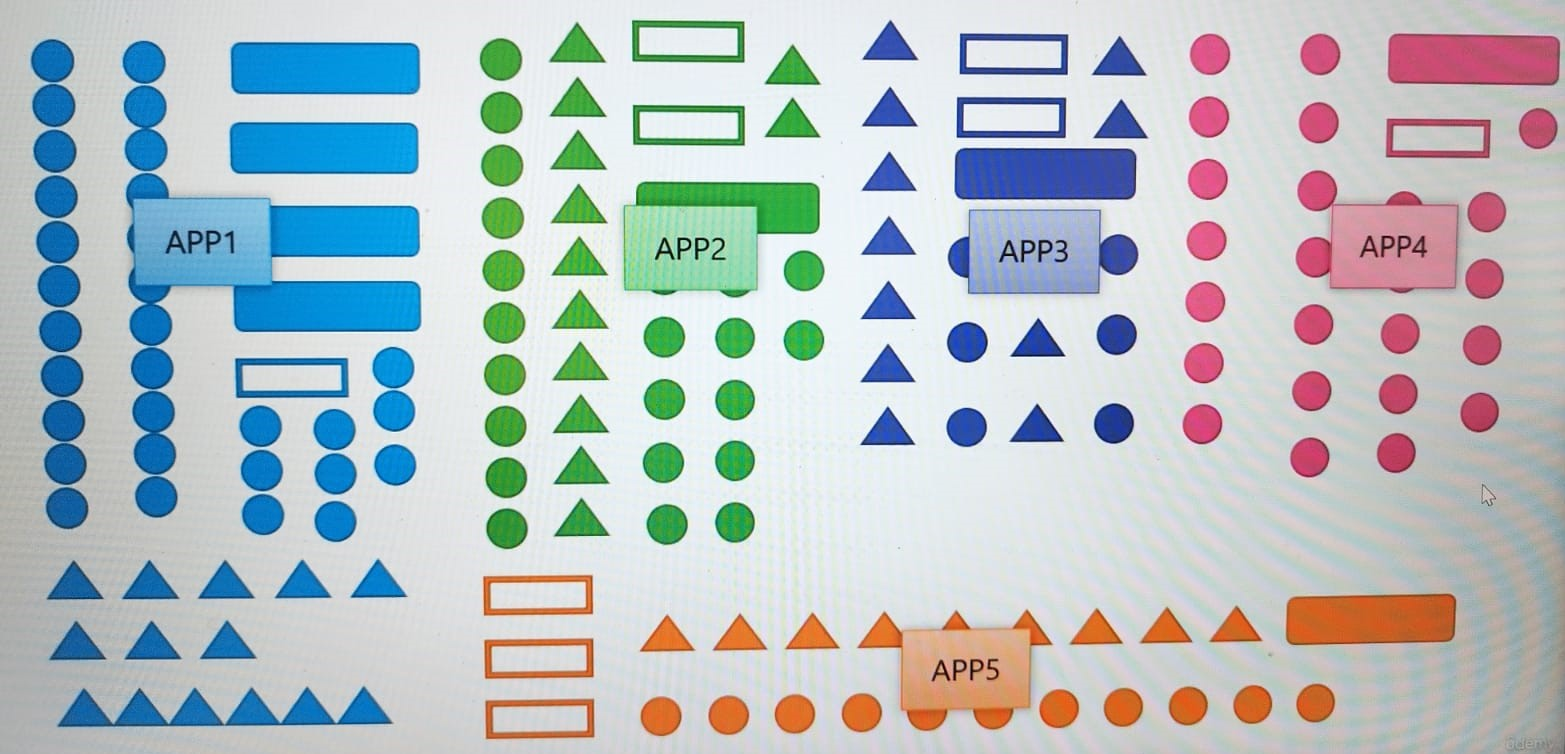
\includegraphics[width=\textwidth]{pictures/sch4.jpg}
\end{figure}

Filtering by functionality:

\begin{figure}[H]
    \centering
    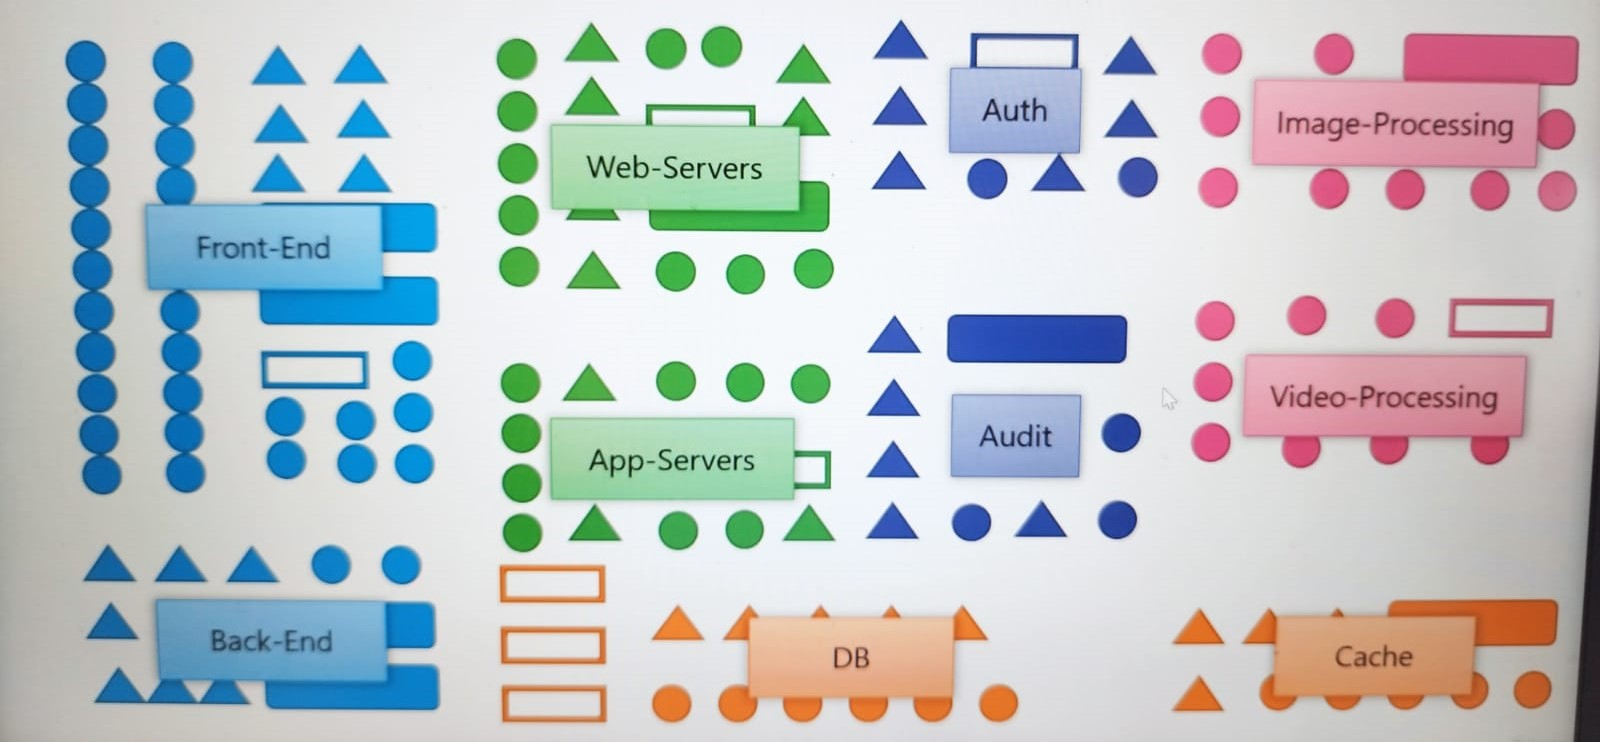
\includegraphics[width=\textwidth]{pictures/sch3.png}
\end{figure}

\subsection{Kubectl commnads with Labels}

To get Objects filtered by labels:
\begin{codetemplate}{}
\begin{verbatim}
$ kubectl get <object> --selector [-l] key=value
\end{verbatim}
\end{codetemplate}

It is possible to filter by different labels:
\begin{codetemplate}{}
\begin{verbatim}
$ kubectl get <object> -l key1=value1 -l key2=value2 ... -l keyN=valueN
\end{verbatim}
\end{codetemplate}

\subsection{Annotations}

\href{https://kubernetes.io/docs/concepts/overview/working-with-objects/annotations/}{Official K8s Doc}

Annotations are used to record other details for informative purpose. For example: tool details, name, version, build info, owner contact, etc. we can use Kubernetes annotations to attach arbitrary non-identifying metadata to objects. Clients such as tools and libraries can retrieve this metadata. we can use either labels or annotations to attach metadata to Kubernetes objects. Labels can be used to select objects and to find collections of objects that satisfy certain conditions. In contrast, annotations are not used to identify and select objects.

%======================================================
\newpage
\section{Pod Scheduling}

\subsection{Manual Scheduling}

In this section we will see how manually scheduling a pod on a Node, what do we do when we do not have a kube-scheduler in the cluster? So we should schedule the pods yourself.

Let's start with Pod definition. Every Pod has a filed called \textbf{nodeName (.spec.nodeName)}, which by default it is not set. we do not typically specify this field when we create the pod manifest file, K8s adds it automatically. 

The kube-scheduler goes through all the pods and looks for those that do not have this property set, those are the candidates for scheduling. It then identifies the right Node for the Pod by running the scheduling algorithm. Once identified, it schedules the Pod on the Node by setting the \textbf{nodeName (.spec.nodeName)} property to the name of the Node. 

So if there is no kube-scheduler to monitor and schedule nodes, what happens? The Pods will be always in a pending state, until we manually assign pods to Nodes yourself. And the easiest way to schedule a pod without kube-scheduler is setting the \textbf{nodeName} field to the name of the node while creating the Pod. And then the Pod will be assigned to the specified Node. 

\begin{codetemplate}{}
\begin{verbatim}
apiVersion: v1
kind: Pod
metadata:
  name: nginx
spec:
  containers:
  -  image: nginx
     name: nginx
  nodeName: node01
\end{verbatim}
\end{codetemplate}

You only can specify the \textbf{nodeName} in creation time, what if the pod is already created and we want to assign the Pod to another Node? K8s will allow we the modify the \textbf{nodeName} assigned to a Pod by another way: creating a \textbf{Binding} Object and send a POST request to the pod's binding API. Thus mimicking what the actual kube-scheduler does. In the \textbf{Binding} Object we specify the \textbf{.target.node} as the name of the Node.

\begin{blocktemplate}{NOTE:}
Also we can delete and create a new Pod with the same name. If the Pod is not assigned to any Port, it will have the Node to \verb|<none>| but anyway we cannot reasign it to another node, we have to delete it and create it again. Or use the command replace!
\end{blocktemplate}

\begin{blocktemplateIII}{NOTE:}
With the command \verb|kubectl replace -f| we can replace an object created by injecting them the specified in a YAML or JSON file, and then K8s will apply the changes. But it is a best practice to at first get the object, edit it and try to apply it.

In case of Node, we said that is not possible to modify them, but if we use the option \verb|--force| the object will be automatically deleted and recreated with the specified changes, it does not matter what they were.
\begin{figure}[H]
    \centering
    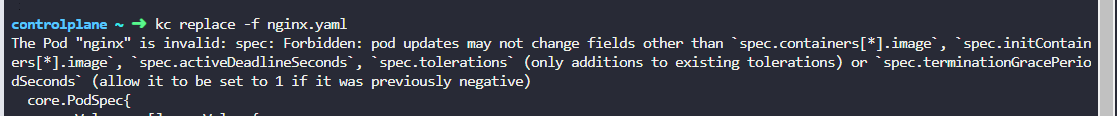
\includegraphics[width=\textwidth]{pictures/sch1.png}
\end{figure}
\begin{figure}[H]
    \centering
    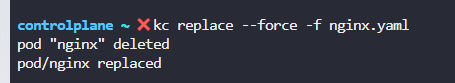
\includegraphics[scale=0.6]{pictures/sch2.png}
\end{figure}
\end{blocktemplateIII}

\begin{codetemplate}{}
\begin{verbatim}
apiVersion: v1
kind: Binding
metadata:
    name: nginx
taget:
    apiVersion: v1
    kind: Node
    name: node02
\end{verbatim}
\end{codetemplate}

Then we have to send a \textbf{POST} request to the Pod's binding API with the data defined in the Binding Object \textbf{YAML} file buut in \textbf{JSON} format. So we must convert the YAML file into the equivalent JSON.

To get the Cluster Nodes:

\begin{codetemplate}{}
\begin{verbatim}
$ kubectl get nodes
\end{verbatim}
\end{codetemplate}

\subsection{Taints \& Tolerations}

\href{https://kubernetes.io/docs/concepts/scheduling-eviction/taint-and-toleration/}{Official K8s Doc}

\subsubsection{Introduction}

In this section we will talk about th\textbf{Pod-Node} relationship and how we can restrict what Pods are placed on what Nodes. 

To understand Taints \& Tolerations easily, we are going to see a vegetables garden example. Imagine we have a vegetable garden, where we have vegetables and insects. If we do not want the flies to get on the plant, we spray the plant with a repellent spray \textbf{(a taint)} we know the fly is intolerant, so the \textbf{taint} would made the fly goes away. However, there are a lots of insects that are tolerant to this smell, and the taint does not really affect them, so they end up in our plant.

So in this example, there are two things that decide if an insect can get a plant:

\begin{itemize}
    \item \textbf{Taint} used on a plant
    \item The insect \textbf{Toleration} to that particular Taint
\end{itemize}

Taking back to K8s, the Nodes are the plants on the vegetables garden (K8s Cluster) and the Pods are the insects. Taints and Tolerations are used to set restrictions on what Pods can be scheduled on a Node.

So imagine the following situation, we have 3 Nodes: Node 1, Node 2 and Node 3. Also we have 4 Pods: A, B, C and D. So if nothing is specified, K8s will distribute the load for example:

\begin{itemize}
    \item \textbf{Node 1:} A
    \item \textbf{Node 2:} B
    \item \textbf{Node 3:} C \& D
\end{itemize}

But now imagine that \textbf{Node A} is so important to the stability of the Cluster, so we have to prevent Pods to run in the Node A, how? \textbf{Placing a taint on the Node A}, let's call it \textbf{blue}, so app=blue. \textbf{By default, Pods have no toleration} which means unless specified otherwise, any Pod can tolerate any Taint. So this is the solution of our problem!!!

But we can imagine our next requirement, because humanity is insatiable, we would want that certain Pods can run on a Node and not others. That's the reason why we need \textbf{Tolerations}. Imagine that we want that in \textbf{Node 2} we want that Pods A and B runs but C and D not. So we have to apply a \textbf{Taint to Node 2}, for example tier=front-end, and then we have to add the \textbf{Toleration} tier=front-end to the Pods A and B and not to C and D.

As we said, the kube-scheduler works this way \ref{Scheduling}. 

\subsubsection{kubectl commands}

\textbf{To taint a Node}
\begin{codetemplate}{}
\begin{verbatim}
$ kubectl taint nodes <node-name> key=value:taint-effect
\end{verbatim}
\end{codetemplate}

Tains effectas can be:
\begin{itemize}
    \item \verb|NoSchedule:| Pods that do not tolerate the taint will not be scheduled on the node.
    \item \verb|PreferNoSchedule:| Kubernetes will try to avoid scheduling Pods that do not tolerate the taint on the node if there are other supported nodes.
    \item \verb|NoExecute:| Pods that do not tolerate the taint will be evicted from the node if they are already running, and they will be rescheduled into another nodes if it is possible.
\end{itemize}

\href{https://kubernetes.io/docs/concepts/scheduling-eviction/taint-and-toleration/}{Official Doc} | \verb|kubectl taint --help|

\underline{EXAMPLE:}
\begin{codetemplate}{}
\begin{verbatim}
$ kubectl taint nodes node01 app=blue:NoSchedule
\end{verbatim}
\end{codetemplate}

The \textbf{taint-effect} defines what would happen to the Pods if they do not tolerate the taint. There are three taint effects:

\begin{itemize}
    \item \textbf{NoSchedule:} the Pods do not be scheduled on the Node, actually what we have been discussing
    \item \textbf{PreferNoSchedule:} the system will try to avoid placing a Pod without Toleration to that taint on the Node, but that is not guaranteed
    \item \textbf{NoExecute:} new Pods will not be scheduled on the Node, and existing Pods on the Node, if there are any, will be evicted if they not tolerate that Taint (killed and rescheduled on another Node)
\end{itemize}

\textbf{To add Toleration to a Pod} | \href{https://kubernetes.io/docs/concepts/scheduling-eviction/taint-and-toleration/}{Official Doc}

Define in it YAML file the section \textbf{.spec.tolerations} which will be a list:

\label{NodeSelector}
\begin{codetemplate}{}
\begin{verbatim}
apiVersion: v1
kind: Pod
metadata:
    name: myapp-pod
spec:
    containers:
    - image: nginx:latest
      name: nginx-container
    tolerations:
    - effect: "NoSchedule" | "PreferNoSchedule" | "NoExecute"
      key: "key" 
      operator: "Equal" | "Exists"
      value: "value"
\end{verbatim}
\end{codetemplate}

\begin{blocktemplateIII}{WARNING}
It is mandatory to encode all the values specified in tolerations in double codes ("")!
\end{blocktemplateIII}

\begin{blocktemplateII}{NOTE 1}
Remember that \textbf{Taints \& Tolerations} do not tell Pods to go to a particular Node, because a Pod has a Taint it does not mean that it should go to the Nodes with the Taint, it is not the purpose. Instead, it tells the Nodes to only accept Pods with certain tolerations.

If we requirement is to restrict a Pod to certain Nodes, it is provided by another concept called as \textbf{NodeAffinity}.
\end{blocktemplateII}

Operator could be:
\begin{itemize}
    \item \textbf{Equal:} Pod accepts to deploy in nodes with specific Taint value specified.
    \item \textbf{Exists:} Pod accepts to deploy in nodes with that Taint specified.
\end{itemize}

\subsubsection{Taint in Master Nodes (control-plane Nodes)}

So far we have only been referrring to the \textbf{Worker Nodes}, but we also have \textbf{Master Nodes (control-plane Nodes)} in the Cluster, which is technically just another Node that has all the capabilities of hosting a Pod plus it runs all the management software. However, \textbf{kube-scheduler never schedule Pods on the Master Nodes (control-plane Nodes)}. Why is that?

When the K8s Cluster is first set up, a \textbf{Taint} is set on the \textbf{Master Node} / \textbf{Master Nodes (control-plane Nodes)} automatically, that prevent any Pods from being scheduling on these Nodes. we can revert this configuration as required, but it is recommended to not do it, not deploy application workloads on a \textbf{Master Service}.

\begin{codetemplate}{}
\begin{verbatim}
$ kubectl get node kubemaster | grep -i taint
\end{verbatim}
\end{codetemplate}

\subsection{Node Selector}

\href{https://kubernetes.io/docs/concepts/scheduling-eviction/assign-pod-node/}{Official K8s Doc}

\subsubsection{Introduction to Node Selectors}

Let's start with a simple example. We have 3 Nodes in the Cluster, for which two are smaller Nodes with lower hardware resources, and one of them is a larger Node configured with higher resources. we have also different kinds of workloads running in we Cluster, we would like to dedicate the data processing workloads that require higher horsepower to the larger Node. However, in the current default setup, any pods can go to any nodes indifferently.

So to solve this, we can set a limitation on the Pods, so that they only run on particular Nodes and there are two ways of do this: \textbf{nodeSelector} and

\subsubsection{Pod Configuration}
\textbf{nodeSelector} is the simplest way, we only should to add at Pod definition the specification \textbf{.spec.nodeSelector}:

\begin{codetemplate}{}
\begin{verbatim}
apiVersion: v1
kind: Pod
metadata:
    name: myapp-pod
spec:
    containers:
    - image: nginx:latest
      name: nginx-container
    nodeSelector:
        size: large
\end{verbatim}
\end{codetemplate}

But wait a minute, where did the size large come from? How does K8s know which is the larges node? Deep down we know the answer, it is a label assigned to a Node. The kube-scheduler uses this labels assigned to Nodes to match and identify the right Node to place the pods on.

\subsubsection{Node Configuration}

\href{https://kubernetes.io/docs/tasks/configure-pod-container/assign-pods-nodes/}{Oficial K8s Documentation}


\textbf{To configure labels in Nodes:}
\begin{codetemplate}{}
\begin{verbatim}
$ kubectl label node <node-name> <label-key>=<label-value>
\end{verbatim}
\end{codetemplate}

\textbf{To see labels in Nodes:}
\begin{codetemplate}{}
\begin{verbatim}
$ kubectl get node --show-labels
\end{verbatim}
\end{codetemplate}

\underline{EXAMPLE:}
\textbf{To configure labels in Nodes:}
\begin{codetemplate}{}
\begin{verbatim}
$ kubectl label nodes node01 size=large
\end{verbatim}
\begin{codetemplate}{}
\begin{verbatim}
apiVersion: v1
kind: Pod
metadata:
    name: myapp-pod
spec:
    containers:
    - image: nginx:latest
      name: nginx-container
    nodeSelector:
        size: large
\end{verbatim}
\end{codetemplate}

\end{codetemplate}

\subsection{Affinity and anti-Affinity}

\href{https://kubernetes.io/docs/concepts/scheduling-eviction/assign-pod-node/}{Official K8s Doc}

\subsubsection{Introduction to Node Affinity}

Continuing with the decision of with Pods goes to what Nodes. What happens with complex configuration? For example, if we would decide to put a Pod on a large or medium node, or put a Pod in every Node that are not small. we cannot achieve this using Node Selectors, we have to use \textbf{Node Affinity}

The primary purpose of \textbf{Node Affinity} is to ensure that Pods are hosted on particular Nodes. It provides us with advances capabilities to limit Pod placement on specific Nodes. But great power comes great complexity. Looks what we have to define to do the same as \ref{NodeSelector}: set than a Pod can only deploy in large Nodes:

\begin{codetemplate}{pod-only-largeNodes.yaml}
\begin{verbatim}
apiVersion: v1
kind: Pod
metadata:
    name: myapp-pod
spec:
    containers:
    - image: nginx:latest
      name: nginx-container
    affinity:
        nodeAffinity:
            requiredDuringSchedulingIgnoredDuringExecution:
                nodeSelectorTerms:
                - matchExpressions:
                  - key: size
                    operator: In
                    values:
                    - large
\end{verbatim}
\end{codetemplate}

Let's analize it a little bit closer, under .spec we have .spec.affinity, and then .spec.affinity.nodeAffinity under that. Then we have a property that seems like a sentence (it does no not need definition). The we have nodeSelectorTerms and that is an array where we have to specify if the specified next must be fullfiled or not. The last key-value pairs define the key, the operator because we want that key in Nodes and the value. Easy peasy.

If we want our pod be deployed on large and medium Pods, we only need to add the following value:

\begin{codetemplate}{pod-large-mid-Nodes.yaml}
\begin{verbatim}
apiVersion: v1
kind: Pod
metadata:
    name: myapp-pod
spec:
    containers:
    - image: nginx:latest
      name: nginx-container
    affinity:
        nodeAffinity:
            requiredDuringSchedulingIgnoredDuringExecution:
                nodeSelectorTerms:
                - matchExpressions:
                  - key: size
                    operator: In
                    values:
                    - large
                    - medium
                    
\end{verbatim}
\end{codetemplate}

If we want our Pod only to not be deployed in small Nodes, we can define the Node Affinity:

\begin{codetemplate}{pod-notSmallNodes.yaml}
\begin{verbatim}
apiVersion: v1
kind: Pod
metadata:
    name: myapp-pod
spec:
    containers:
    - image: nginx:latest
      name: nginx-container
    affinity:
        nodeAffinity:
            requiredDuringSchedulingIgnoredDuringExecution:
                nodeSelectorTerms:
                - matchExpressions:
                  - key: size
                    operator: NotIn
                    value:
                    - small
                    
\end{verbatim}
\end{codetemplate}

If we want that Pods only deploy in Nodes with size label defined:

\begin{codetemplate}{pod-notSmallNodes.yaml}
\begin{verbatim}
apiVersion: v1
kind: Pod
metadata:
    name: myapp-pod
spec:
    containers:
    - image: nginx:latest
      name: nginx-container
    affinity:
        nodeAffinity:
            requiredDuringSchedulingIgnoredDuringExecution:
                nodeSelectorTerms:
                - matchExpressions:
                  - key: size
                    operator: Exists
                    
\end{verbatim}
\end{codetemplate}

There are a number of other operators as well, check de official documentation for specific details: \href{https://kubernetes.io/docs/concepts/scheduling-eviction/assign-pod-node/}{Official K8s Documentation}. But the most used are:
\begin{itemize}
    \item \textbf{In:} have the label and with the value.
    \item \textbf{NotIn:} have the label but with different value.
    \item \textbf{Exists:} just have the label.
    \item \textbf{DoesNotExist:} just not have the label.
\end{itemize}

\subsubsection{Node Affinity Types}

So when the Pods are created, these rules are considered and the Pods are placed onto the right Nodes, but what happens when \textbf{nodeAffinity} could not match a Node with a given expression? And what happens when the pods are running and the labels on a Node are changed? All these are specified in the \textbf{.spec.affinity.nodeAffinity...}. This long sentence specifies what happens with the Affinity.

There are two states in the life-cycle of a Pod when considering \textbf{Node Affinity}:
\begin{itemize}
    \item \textbf{DuringScheduling:} state when the Pod does not exist and it is created for the first time
    \item\textbf{DuringExecution:} state when the Pod has been running and change is made in the environment that affects \textbf{NodeAffinity} (such as a change in the label of a Node)
\end{itemize}

There are three options to determine the severity of the affinity:
\begin{itemize}
    \item \textbf{Required:} it is absolutely necessary to have a Node with the specified labels, so if the label is not find, the Pod won't be deployed.
    \item\textbf{Preferred:} it is preferred to have a Node with the specified labels, and if the label is not found but kube-scheduler do not find available nodes with the label, the rule will be simply ignored.
    \item \textbf{Ignored:} pods will continue to run and any changes in Node Affinity will not impact them once they are scheduled.
\end{itemize}

The most commonly used are:
\begin{itemize}
    \item requiredDuringSchedulingIgnoredDuringExecution
    \item preferredDuringSchedulingIgnoredDuringExecution
    \item requiredDuringSchedulingRequiredDuringExecution
\end{itemize}

\begin{table}[H]
\begin{tabular}{| m{3cm} | m{4cm} | m{4cm} |}
\hline
& \textbf{DuringScheduling} & \textbf{DuringExecution} \\ \hline
Type 1 & Required & Ignored \\ \hline
Type 2 & Preferred & Ignored \\ \hline
Type 3 & Required & Required \\ \hline
\end{tabular}
\end{table}

\subsubsection{Inter-pod affinity and anti-affinity}
Inter-pod affinity and anti-affinity allow we to constrain which nodes our Pods can be scheduled on based on the labels of \textbf{Pods} already running on that node, instead of the node labels.

Inter-pod affinity and anti-affinity rules take the form "this Pod should (or, in the case of anti-affinity, should not) run in an X if that X is already running one or more Pods that meet rule Y". we express these rules (Y) as label selectors with an optional associated list of namespaces. Pods are namespaced objects in Kubernetes, so Pod labels also implicitly have namespaces. Any label selectors for Pod labels should specify the namespaces in which Kubernetes should look for those labels.

You express the topology domain (X) using a \verb|topologyKey|, which is the key for the node label that the system uses to denote the domain.

\begin{blocktemplateII}{NOTE}
Pod anti-affinity requires nodes to be consistently labeled, in other words, every node in the cluster must have an appropriate label matching \verb|topologyKey|. If some or all nodes are missing the specified \verb|topologyKey| label, it can lead to unintended behavior.
\end{blocktemplateII}

Tyoes if inter-pod affinity and anti-affinity:
\begin{itemize}
    \item \verb|requiredDuringSchedulingIgnoredDuringExecution|
    \item \verb|preferredDuringSchedulingIgnoredDuringExecution|
\end{itemize}

To use inter-pod affinity, use the \verb|affinity.podAffinity| field in the Pod spec. For inter-pod anti-affinity, use the \verb|affinity.podAntiAffinity| field in the Pod spec.

In the followin example, we define one Pod affinity rule and one Pod anti-affinity rule. The Pod affinity rule uses the "hard" 
\verb|requiredDuringSchedulingIgnoredDuringExecution|, while the anti-affinity rule uses the "soft" 
\verb|preferredDuringSchedulingIgnoredDuringExecution|. 

The affinity rule specifies that the scheduler is allowed to place the example Pod on a node only if it is labeled with \verb|topology.kubernetes.io/zone| and there are Pods running with the label \verb|security=S1|. As well it will try to avoid deploy pods on nodes with other pods running and label \verb|security=S2|

\begin{codetemplate}{}
\begin{verbatim}
apiVersion: v1
kind: Pod
metadata:
  name: with-pod-affinity
spec:
  affinity:
      podAffinity:
        requiredDuringSchedulingIgnoredDuringExecution:
        - labelSelector:
            matchExpressions:
            - key: security
              operator: In
              values:
              - S1
          topologyKey: topology.kubernetes.io/zone
      podAntiAffinity:
        preferredDuringSchedulingIgnoredDuringExecution:
        - weight: 100
          podAffinityTerm:
            labelSelector:
              matchExpressions:
              - key: security
                operator: In
                values:
                - S2
            topologyKey: topology.kubernetes.io/zone
  containers:
  - name: with-pod-affinity
    image: registry.k8s.io/pause:2.0                     
\end{verbatim}
\end{codetemplate}

Kubernetes includes an optional \verb|matchLabelKeys| or \verb|mismatchLabelKeys| field for Pod affinity or anti-affinity. The field specifies keys for the labels that should match with the incoming Pod's labels, when satisfying the Pod (anti)affinity. 
It sets the existing pods that will be taken into Pod (anti)affinity calculation. And the oposite for \verb|mismatchLabelKeys|, they will take into account all pods except the ones with the labels specified.

\begin{codetemplate}{}
\begin{verbatim}
apiVersion: apps/v1
kind: Deployment
metadata:
  name: application-server
...
spec:
  template:
    spec:
      affinity:
        podAffinity:
          requiredDuringSchedulingIgnoredDuringExecution:
          - labelSelector:
              matchExpressions:
              - key: app
                operator: In
                values:
                - database
            topologyKey: topology.kubernetes.io/zone
            # Only Pods from a given rollout are taken into consideration when calculating pod affinity.
            # If we update the Deployment, the replacement Pods follow their own affinity rules
            # (if there are any defined in the new Pod template)
            matchLabelKeys:
            - pod-template-hash
\end{verbatim}
\end{codetemplate}

\subsection{Resource Requirements \& Limits}

\href{https://kubernetes.io/docs/concepts/configuration/manage-resources-containers/}{Official K8s Documentation}

\begin{blocktemplateIII}{WARNING}
Resources (required and limits) are \textbf{always} defined by \textbf{container}, \textbf{NOT BY POD}
\end{blocktemplateIII}

\subsubsection{Introduction}
Let's imagine a Cluster with 3 Worker Nodes available, each Node has a set of CPU and memory resources available. Every Pod requires a set of resources to run, and when a Pod is running on a Node, it consumes the resources available on that Node. As we discuss before, it is the \textbf{kube-scheduler} that decides which Node a Pod goes to, taking into account the amount of resources required by a Pod and those available on the Nodes. It identifies the best Node to place a Pod on in function of the resting resources if the Pod runs on it (explained in section \ref{Scheduling}.

So if we have a Pod which needs 1 core CPU and 2Gi of Memory, without no Affinity Policies, Taints, Node Selector, etc. It will deploy randomly in one of the 3 nodes. 

If we get another, it would be allocated in another Node, because for kube-scheduler it would be better, since it would have more capacity once the Pod is running on it.

It would be done until all Nodes capacity is full, or since a Pod cannot run in any Node, because they have no enough resources, so the kube-scheduler holds back scheduling the Pod, so we could see it in a Pending state. If we look at the events we would see there is an insufficient CPU / Memory.

\subsubsection{Resources types}
\paragraph{CPU}

Limits and requests for CPU resources are measured in CPU units. In Kubernetes, 1 CPU unit is equivalent to 1 physical CPU core, or 1 virtual core, depending on whether the node is a physical host or a virtual machine running inside a physical machine.
\begin{itemize}
    \item \textbf{Floats:} 1.0, 0.5, 1.75, 0.005
     \item \textbf{Millicpu (in double quotes):} "1000m", 500m, 1750m, 5m
\end{itemize}

\paragraph{Memory}

Memory refers to RAM. It can be defined as:
\begin{itemize}
    \item \textbf{Plain Integers:}
    \item \textbf{Power-of-ten equivalents (with double quote):}
    \begin{itemize}
        \item 1m=1e-3
        \item 1.5k=1.5e3
        \item 0.75M=0.75e6
        \item 1G=1e9
    \end{itemize}
    \item \textbf{Power-of-two equivalents (with double quote):}
    \begin{itemize}
        \item 1Ki=$1x2^{10}$ (1 Kibibyte)
        \item 1.5Mi=$1.5x2^{20}$ (1.5 Mebibytes)
        \item 2.7Gi=$2.7x2^{30}$ (2.7 Gibibytes)
        \item 0.8Ti=$0.8x2^{40}$ (0.8 Tebibytes)
    \end{itemize}
\end{itemize}

\begin{blocktemplateI}{NOTE}
Just to remember, and it applies to all mesures:
\begin{itemize}
    \item Kilobyte = $10^3$
    \item Megabyte = $10^6$
    \item Kibibyte = $2^{10}$
    \item Mebibyte = $2^{20}$
\end{itemize}

\begin{figure}[H]
    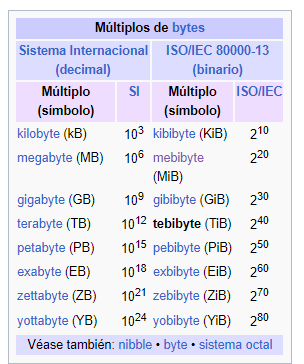
\includegraphics[scale=0.6]{pictures/bib.png}
\end{figure}
\end{blocktemplateI}

\subsubsection{Requests \& Limits}

\begin{blocktemplateIII}{WARNING}
Resources (required and limits) are \textbf{always} defined by \textbf{container}, \textbf{NOT BY POD}. So each container in a Pod have its resources definition (requests and limits).
\end{blocktemplateIII}

\paragraph{Requests}

The amount of CPU and Memory \textbf{required} for a \textbf{Container} to run, so the kube-scheduler will never allocate a Pod in a Node with less resources than the \textbf{sum of required resources of all the containers in Pod}.

\begin{codetemplate}{}
\begin{verbatim}
apiVersion: v1
kind: Pod
metadata:
    name: myapp-pod
spec:
    containers:
    - image: nginx:latest
      name: nginx-container
      resources:
        requests:
            cpu: 1.0
            memory: "2Gi"
\end{verbatim}
\end{codetemplate}

\paragraph{Limit}

Says a Pod are allocated into a Node based on the Required Resources. The Pod container starts consuming 1 CPU on a Node, actually it can go up and consume as much resources as it requires and that suffocates the native processes on the Node or other containers of resources.

That's the reason we can set a limit for the resource usage on Pods. The limit has different behaviour depending of wheter is CPU or Memory:
\begin{itemize}
    \item \textbf{CPU:} The CPU limit cannot be exceeded, so if the container needs more CPU, it wouldn't have it, it would work slower.
    \item \textbf{Memory:} A container can use more memory resources than its limit, but if it is detected the Pod will be automatically \textbf{Terminated} with an \textbf{OOM (Out of Memory)}. This is because once memory is used by a Pod, the only way to release it is killing the Pod.
\end{itemize}

\begin{codetemplate}{}
\begin{verbatim}
apiVersion: v1
kind: Pod
metadata:
    name: myapp-pod
spec:
    containers:
    - image: nginx:latest
      name: nginx-container
      resources:
        requests:
            cpu: 1.0
            memory: "2Gi"
        limits:
            cpu: "1750m"
            memory: "2.75Gi"
\end{verbatim}
\end{codetemplate}

\begin{blocktemplateII}{NOTE}
We can define only limits or only requests in the resources of a container. But we would have to assume the consequences, but K8s allow it.
\end{blocktemplateII}

\subsubsection{Ideal Scenario for CPU}
So far it seems completely good for our environment, but don not we think it can be so inefficient sometimes? Imagine we have a Node with 2 Pods running:
\begin{enumerate}
    \item \textbf{Pod 1:} request 1CPU, limit 3CPU
    \item \textbf{Pod 1:} request 2CPU, limit 4CPU
\end{enumerate}

So at one time, Pod 1 are consuming 3CPU (because it cannot consume more), but it needs more CPU at this moment to work properly. On the other hand, Pod 2 are consuming only 0.5CPU, because it does not need more resources at that moment. Is not this an inefficiency?

The answer is yes, it is, that's why the \textbf{Ideal Scenario} is:
\begin{itemize}
    \item Define requests
    \item Do not define limits
\end{itemize}

This way any Pod can consume as many CPU cycle as available. So it is the most ideal setup, of course there are cases where we absolutely may want to limit a Pod of resources and in that case we have to set limits. For example the labs used for practise this course. All the labs are hosted as containers on a K8s Cluster, and of course, since it were made accessible to public, the containers have limits, to prevent users misusing the infrastructure to for example Bitcoin mining or other resource consuming activities.

Another advice is to set requests always, because if not, Pods can be allocated in Nodes without enough resources to run it, and if the containers have no limits it can be chaos.


\subsubsection{Default Configuration}

By default K8s does not have a CPU or a memory request or limit set, so this means that any Pod can consume as much resources as required on any Node, suffocating other Pods or processes that are running on the Node.

\subsubsection{Changing Default Configuration, LimitRange Object}

\href{https://kubernetes.io/docs/concepts/policy/limit-range/}{Official K8s Doc}

How can we ensure that every Pod has some default set? This is possible with \textbf{LimitRange} Object. By default, containers run with unbounded compute resources on a Kubernetes cluster. Using Kubernetes resource quotas, administrators (also termed cluster operators) can restrict consumption and creation of cluster resources (such as CPU time, memory, and persistent storage) within a specified namespace. Within a namespace, a Pod can consume as much CPU and memory as is allowed by the ResourceQuotas that apply to that namespace. As a cluster operator, or as a namespace-level administrator, we might also be concerned about making sure that a single object cannot monopolize all available resources within a namespace..

\begin{codetemplate}{}
\begin{verbatim}
apiVersion: v1
kind: LimitRange
metadata:
    name cpu-resources-constraint
spec:
    limits:
    - default:
        cpu: "500m"
      defaultRequest:
        cpu: "500m"
      max:
        cpu: 1
      min
        cpu: "100m"
      type: Container
\end{verbatim}
\end{codetemplate}

\begin{itemize}
    \item \textbf{default:} defines default limit (if not defined)
    \item \textbf{defaultRequest:} defines default request (if not defined)
    \item \textbf{max:} refers to the maximum CPU that can be defined as request
    \item \textbf{minimum:} refers to the minimum CPU that can be defined as request
\end{itemize}

For memory it is the same:
\begin{codetemplate}{}
\begin{verbatim}
apiVersion: v1
kind: LimitRange
metadata:
    name cpu-resources-constraint
spec:
    limits:
    - default:
        memory: "500m"
      defaultRequest:
        memory: "500m"
      max:
        memory: 1
      min
        memory: "100m"
      type: Container
\end{verbatim}
\end{codetemplate}

\begin{blocktemplateIII}{WARNING 1}
If we define limits on the container definition LimitRange object will be overwritten by this limits.
\end{blocktemplateIII}

\begin{blocktemplateIII}{WARNING 2}
This Objects only affects to newer Pods that are created, so does not affect existing Pods
\end{blocktemplateIII}

\subsubsection{Restrict the total amount of resources}

Is there any way to restrict the total amount of resources that can be consumed by applications in a K8s Cluster? The answer is not by cluster, but yes by Namespace, with \textbf{ResourceQuota} Objects, like we discuss in section \ref{Quota}.

\href{https://kubernetes.io/docs/tasks/administer-cluster/manage-resources/quota-memory-cpu-namespace/}{Official K8s Doc}

\subsection{DaemonSets}

\href{https://kubernetes.io/es/docs/concepts/workloads/controllers/daemonset/}{Official K8s Doc}

\subsubsection{Introduction to DaemonSets}

So far we have deployed different replicas of Pods on different Worker Nodes on Cluster. with the help of ReplicaSet and Deployments we make sure multiple replicas of an instance of Pod are made available across different Worker Nodes. \textbf{DaemonSets} are like ReplicaSets as it helps we deploy multiple instances of Pods, but it runs one copy of our Pod on each Worker Node in our cluster. Whenever a new Node is added to the Cluster, DaemonSet add a replica of the Pod to that Node, an when a Node is removed the Pod is automatically removed.

\begin{figure}[H]
    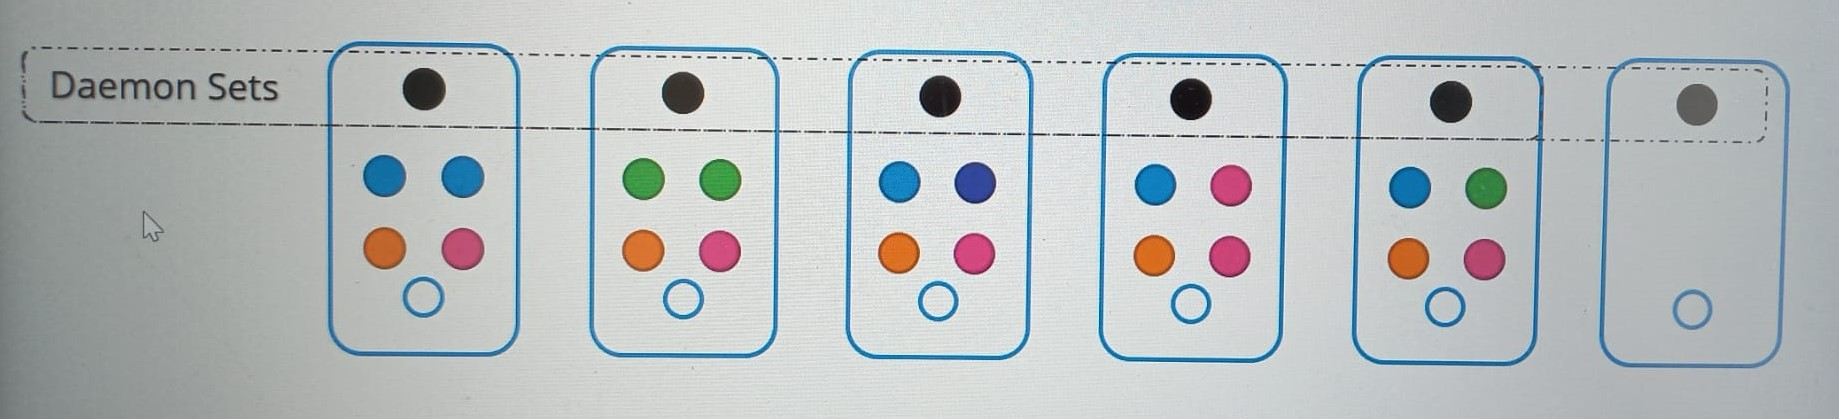
\includegraphics[width=\textwidth]{pictures/ds.png}
\end{figure}

DaemonSet ensures that one copy of a Pod is always present in all Nodes in the Cluster. So for what can it be used? Say we would like to deploy a monitoring agent or a log collector on each of we Nodes in the Cluster. DaemonSet could deploy we monitoring or login agent in each Node of the Cluster.

Another good example of use of DaemonSet is the \textbf{kube-proxy} component, it must be run on each Worker Node on the Cluster, so it is configured as a DeamonSet.

\subsubsection{Defition of DaemonSets}

It is very similar to ReplicaSet definition:

\begin{codetemplate}{daemonSet-definition.yaml}
\begin{verbatim}
apiVersion: apps/v1
kind: DaemonSet
metadata:
    name: monitoring-daemon
spec:
    selector:
        matchLabels:
            app: monitoring-agent
    template:
        metadata:
            name: monitoring-agent
            labels:
                app: monitoring-agent
        spec:
            containers:
            - image: monitoring-agent
              name: monitoring-agent
\end{verbatim}
\end{codetemplate}

\subsubsection{Creation and view of DaemonSets}

\textbf{Creation}
\begin{codetemplate}{}
\begin{verbatim}
$ kubectl create -f daemonset-definition.yaml
\end{verbatim}
\end{codetemplate}

\textbf{View}
\begin{codetemplate}{}
\begin{verbatim}
$ kubectl get ds
\end{verbatim}
\end{codetemplate}

\begin{blocktemplateIII}{WARNING}
This command does not work with daemonSets, I don't know why, it only accepts certain objects
\begin{codetemplate}{}
\begin{verbatim}
$ kubectl create daemonset --help
\end{verbatim}
\end{codetemplate}
\end{blocktemplateIII}

\subsubsection{How dos DaemonSets work?}

\textbf{Before v1.12}, it worked adding the \textbf{NodeSelector} of each Node of the Cluster to every Pod created by DaemonSet. 

\begin{figure}[H]
    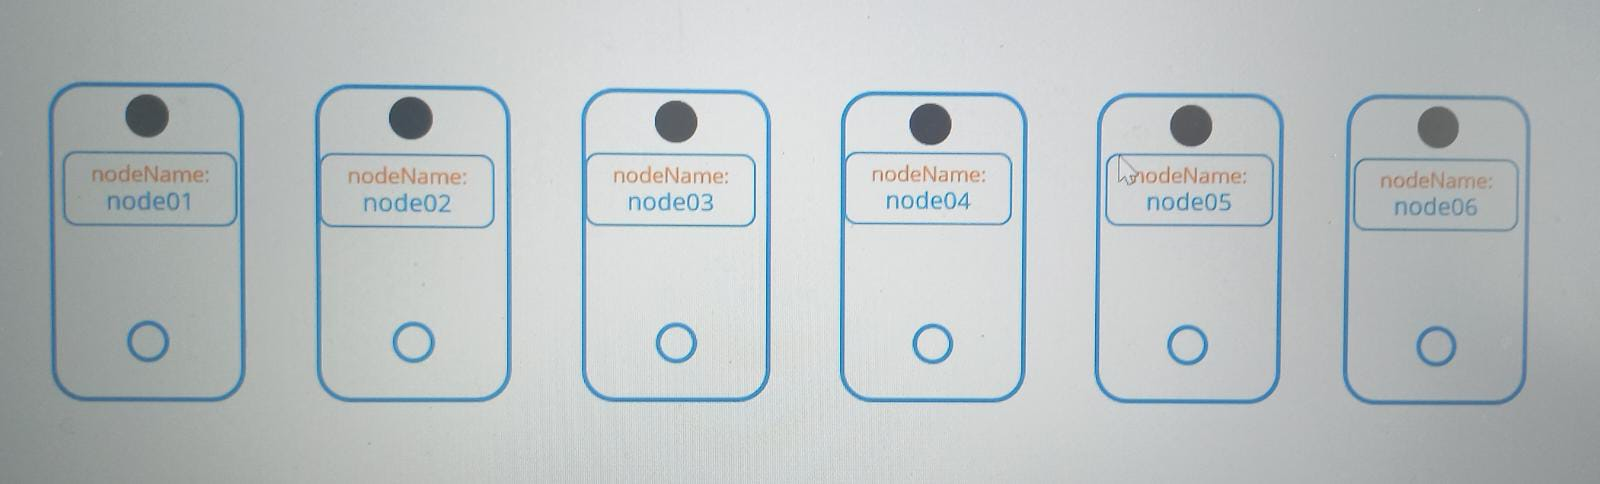
\includegraphics[width=\textwidth]{pictures/ds1.png}
\end{figure}


\textbf{From K8s v1.12 onwards}, the DaemonSet uses the default scheduler and \textbf{NodeAffinity} rules that we have learned to schedule Pods on Nodes.

\subsubsection{Example of DaemonSet - Fluentd}
To build one single log structure in K8s for a couple of apps, or even a dozen, we cannot use basic logging structure, because unfortunately, basic logging doesn’t answer these questions. Data is temporary; any crash or rerun will erase all the previous records.

To address these problems, we need to set it to the node-logging level. Since we can interact with every single object within the node, we can try to make a vertical unique logging system. 

Furthermore, we can implement cluster-level logging by including a node-level logging agent on each node. A logging agent is a dedicated tool that exposes or pushes logs to a backend. Usually, the logging agent is a container that has access to a directory with log files from all of the application containers on that node.

Because the logging agent must run on every node, it’s common to implement it as either a DaemonSet replica: \textbf{Logs Collector: Fluentd}. Fluentd is an ideal solution as a unified logging layer. we just have to open and download the type of logger we need for the project, 
it collects logs both from user applications and cluster components such as kube-apiserver and kube-scheduler. So... It needs to run as \textbf{DaemonSet}.

\begin{blocktemplateIII}{WARNING}
Fluentd is just the log retriever, it won't expose anything, so \verb|curl pod_ip| won't work.
\end{blocktemplateIII}

Example of fluentd daemonset, from \href{https://medium.com/@MetricFire/logging-for-kubernetes-fluentd-and-elasticsearch-9b95c7c64da}{link}:
\begin{codetemplate}{}
\begin{verbatim}
apiVersion: apps/v1
kind: DaemonSet
metadata:
  name: fluentd
  namespace: kube-system
  labels:
	k8s-app: fluentd-logging
	version: v1
	kubernetes.io/cluster-service: "true"
spec:
  selector:
	matchLabels:
  	k8s-app: fluentd-logging
  template:
	metadata:
  	labels:
    	k8s-app: fluentd-logging
    	version: v1
    	kubernetes.io/cluster-service: "true"
	spec:
  	serviceAccount: fluentd # serviceAccountName accepted as well
  	tolerations:
  	- key: node-role.kubernetes.io/master
    	effect: NoSchedule
  	containers:
  	- name: fluentd
    	image: fluent/fluentd-kubernetes-daemonset:v1.3-debian-elasticsearch
    	env:
      	- name:  FLUENT_ELASTICSEARCH_HOST
        	value: "elasticsearch.logging"
      	- name:  FLUENT_ELASTICSEARCH_PORT
        	value: "9200"
      	- name: FLUENT_ELASTICSEARCH_SCHEME
        	value: "http"
      	- name: FLUENT_UID
        	value: "0"
    	resources:
      	limits:
        	memory: 200Mi
      	requests:
        	cpu: 100m
        	memory: 200Mi
    	volumeMounts:
    	- name: varlog
      	  mountPath: /var/log
    	- name: varlibdockercontainers
      	  mountPath: /var/lib/docker/containers
      	  readOnly: true
  	terminationGracePeriodSeconds: 30
  	volumes:
  	- name: varlog
    	hostPath:
      	path: /var/log
  	- name: varlibdockercontainers
    	hostPath:
      	path: /var/lib/docker/containers
\end{verbatim}
\end{codetemplate}

\subsection{Static Pods}
In a really weird scenario, where we are supposing there are no:
\begin{itemize}
    \item kube-apiserver
    \item kube-scheduler
    \item etcd
\end{itemize}

So the kubelet is alone on the sea, it is able to create pods by its own in a very specific way, this pods are called \textbf{Static Pods}. we won't be able to create Deployments, ReplicaSets or other objects. we only will be able to create Pods this way, because the other objects needs some control-plane objects like replication-controller. 

If the connection to the rest of the K8s come back, the kubelet will create a mirror of all the \textbf{Static Pods} on the kube-apiserver, so if we do \verb|kubectl get po|: we will see as well the \textbf{Static Pods}. But we won't be able to edit or delete them using \verb|kubectl|, we must modify or delete them directly from the static file inside kubelet configuration.

\verb|kubeadm| tool makes use of \textbf{Static Pods} to deploy the control-plane components as Pods on a Node. It starts by installing \textbf{kubelet} on all the Master Nodes (control-plane Nodes), then create \textbf{Static Pod} definition files for the various control-plane components, such as: kube-apiserver, kube-controller, etcd, etc.
Then, it places the definition files inside the designated manifest folder and the the kubelets automaticically takes care of deploying
them as \textbf{Static Pods} on the Cluster. This way it avoids to download binaries, configure and run services or worry about the services crashing,
because it will be restarted by the kubelet.

The most common place to store the manifest of these static pods and the one used by \verb|kubeadm| is: \verb|/etc/kubernetes/manifests|. But it could be any directory on the Node, we just need to configure it properly on the \verb|kubelet/config.yaml|, which use to be on: \verb|/var/lib/kubelet/config.yaml|

\begin{blocktemplate}{NOTE}
If we are not sure of where is this path, we can do:
\begin{enumerate}
    \item Check kubelet is running on the node:
\begin{codetemplate}{}
\begin{verbatim}
$ systemctl status kubelet
\end{verbatim}
\end{codetemplate}

    \item Check service configuration:
\begin{codetemplate}{}
\begin{verbatim}
$ ps waux | grep kubelet
\end{verbatim}
\end{codetemplate}

    \item Check the configuration and we will find the \verb|kubelet/config.yaml|
\end{enumerate}
\begin{figure}[H]
    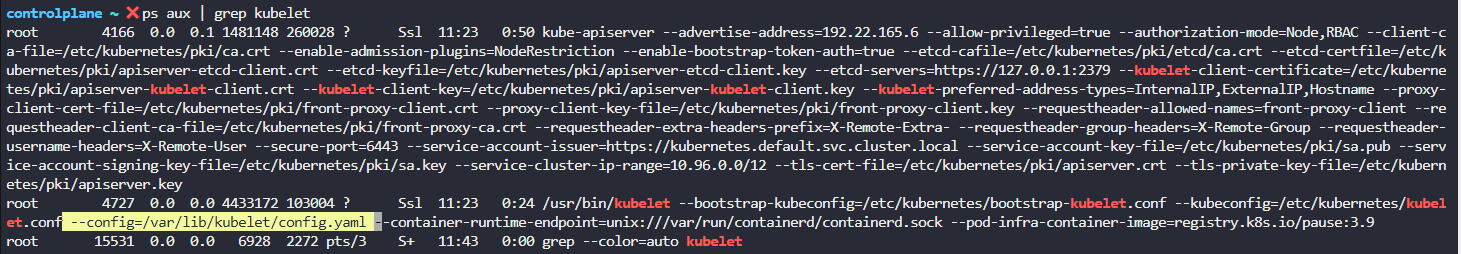
\includegraphics[width=\textwidth]{pictures/kubelet-config.png}
\end{figure}
\end{blocktemplate}

So we can check inside the config file where the kubelet reads for the manifests:
\begin{codetemplate}{}
\begin{verbatim}
$ cat /var/lib/kubelet/config.yaml | grep -i static
\end{verbatim}
\end{codetemplate}

So when we do \verb|kubectl get pods -n kube-system| we will see all the control-plane services running as pods.

\begin{blocktemplateI}{NOTE}
If we pay attention, is that the reason why if we remove some of the control-plane pods, it is automatically recreated but it does not have any deployment, statefulset, daemonset or replicaset controlling them.

Well, take care of \textbf{kube-proxy}, because it is the exception, it is a \textbf{daemonSet}.
\end{blocktemplateI}

\subsection{Multiple Schedulers}

\href{https://kubernetes.io/docs/tasks/extend-kubernetes/configure-multiple-schedulers/}{Official K8s Doc}

\subsubsection{Introduction}

So far, we have seen how one single scheduler works in a K8s Cluster, it has an algorithm that distribute Pods across Nodes, taking into account Taint \& Tolerations, NodeSelector, NodeAffinity, Resources, etc. But what if we need more? If we have an application that requires some additional checks? \textbf{K8s is highly extensible}, we can\textbf{ write our own K8s scheduler program}, package it and deploy it as the default scheduler or as an additional scheduler in the K8s Cluster. That way some applications can use the default K8s scheduler and others can use our custom schedulers (you can configure more than one). A K8s Cluster accepts multiple schedulers at a time.

\subsubsection{Defining schedulers}

When creating a Pod (or a Pod Object Manager). we can instruct K8s to have the Pod scheduled by a specific scheduler, so the different schedulers must have different names, in order we can identify them as separate schedulers. The default scheduler is named default scheduler XD, and this name is configured in the \textbf{kube-scheduler} configuration file that looks like this:

\begin{codetemplate}{scheduler-config.yaml}
\begin{verbatim}
apiVersion: kubescheduler.config.k8s.io/v1
kind: KubeSchedulerConfiguration
profiles:
- schedulerName: default-scheduler
leaderElection:
    leaderElect: true
    resourceNamespace: kube-system
    resourceName: lock-object-my-scheduler
\end{verbatim}
\end{codetemplate}

For other schedulers, we can create a similar file, changing the \textbf{schedulerName value}.

The \textbf{leaderElection} is configured because if there are multiple copies of an scheduler running on different Nodes only one can be active at a time. So this optioon helps using a leader who will lead the scheduling activities

\subsubsection{Creating new schedulers}

There are two ways to create new schedulers:

\paragraph{Bad way: as a service in the system}

To create a new scheduler we must use the same \textbf{kube-scheduler binary} mentioned in Section \ref{schduler} but setting the configuration with the YAML file that we have created... we can imagine it is terrible.

\paragraph{Good way: as a Pod in K8s kube-system Namespace}

\begin{codetemplate}{my-custom-scheduler.yaml}
\begin{verbatim}
apiVersion: v1
kind: Pod
metadata:
    name: my-custom-scheduler
    namespace: kube-system
spec:
    containers:
    - command:
      - kube-scheduler
      - --adress=127.0.0.1
      - --kubeconfig=/etc/kubernetes/scheduler.conf
      - --config=/path/to/my-scheduler.yaml
      image: k8s.grc.io/kube-scheduler-amd64:v1.11
      name: kube-scheduler
\end{verbatim}
\end{codetemplate}

\subsubsection{Configuring Pods to consume a custom scheduler}

\begin{codetemplate}{pod-consuming-custom-sch.yaml}
\begin{verbatim}
apiVersion: v1
kind: Pod
metadata:
    name: nginx
spec:
    containers:
    - image: nginx
      name: nginx
    schedulerName: my-custom-scheduler
\end{verbatim}
\end{codetemplate}

\subsubsection{Monitor the correct functioning of a custom scheduler}

\begin{codetemplate}{}
\begin{verbatim}
$ kubectl get events -o wide
\end{verbatim}
\end{codetemplate}

\begin{codetemplate}{}
\begin{verbatim}
$ kubectl logs my-custom-scheduler -n kube-system
\end{verbatim}
\end{codetemplate}

\subsection{Scheduler Profiles}

Scheduling a Pod is not as easy as it seems. Default \textbf{kube-scheduler} follow the process:
\begin{itemize}
    \item Put the Pod to create into the \textbf{scheduling queue}
    \item On this queue, Pods are sorted based on the \textbf{priority} defined directly on the Pod definition (if there is).
\end{itemize}

\begin{blocktemplateI}{NOTE}
You can check on the official documentation how to create \verb|PriorityClass| and assign it to a Pod.
\end{blocktemplateI}

\begin{itemize}
    \item Once the sorted phase, the Pod enter into the \textbf{Filtering Phase}, where Nodes that cannot run the pod because of taints, nodeAffinity, not enough resources, etc. are filtered out.
    \item \textbf{Scoring Phase:} not filtered nodes are scored based on their free resources and presence of the image locally.
    \item \textbf{Binding Phase:} the pod is finally bound to the node with the highest score.
\end{itemize}

All these actions are achieved with certain plugins:
\begin{itemize}
    \item PrioritySort
    \item NodeResourceFit
    \item NodeName
    \item NodeUnschedulable
    \item NodeResourcesFit
    \item ImageLocality
\end{itemize}

So we can define different scheduler profiles to disable and enable different pluggins:

\begin{codetemplate}{}
\begin{verbatim}
apiVersion: kubescheduler.config.k8s.io/v1
kind: KubeSchedulerConfiguration
profiles:
  - plugins:
      score:
        disabled:
        - name: PodTopologySpread
        enabled:
        - name: MyCustomPluginA
          weight: 2
        - name: MyCustomPluginB
          weight: 1
\end{verbatim}
\end{codetemplate}

For more information, check the \href{https://kubernetes.io/docs/reference/scheduling/config/}{Official K8s Documentation}


%======================================================
\newpage
\section{Logging and Monitoring}

In this section we will see how to monitor K8s components as well as the applications hosted in the Cluster. How to view and manage the logs of the Cluster components as well as the application logs.

\subsection{Monitoring Cluster Components}

How do we monitor resource consumtion in K8s, or more important, what would we like to monitor? I would like to know node-level metrics, such as:
\begin{itemize}
    \item The number of nodes in the cluster
    \item How many of them are healthy
    \item Performance Node metrics like CPU, Memory, Network Disk Utilization, etc.
\end{itemize}

Such as Pod level metrics:
\begin{itemize}
    \item Number of replicas of a Pod
    \item The metric consumtion this POds and the state
\end{itemize}

So we need a solution that monitor all these metrics, store them and provides analytics around this data. Unfortunately, K8s does not come with a full-featured built-in monitoring solution. However, there are a number of open-source solutions available such as:
\begin{itemize}
    \item Prometheus
    \item Elastic Stack
    \item Metrics Server
    \item Datadog (private)
    \item Dynatrace (private)
\end{itemize}

Any of the solutions retrieves data of every K8s Node and Pod. All this data are stored in a memory. But to do that, K8s must pass this data in anyway. \textbf{Kubelet} has a subcomponent called \textbf{Container Advisor (CAdvisor)}, this subcomponent is responsible for retreiving performance metrics from pods and exposing them through the kubelet API to make the metrics available for the metrics solution.

\subsubsection{Basic K8s Metrics Server}

\textbf{If we are using Minikube:}
\begin{codetemplate}{}
\begin{verbatim}
$ minikube addons enable metrics-server
\end{verbatim}
\end{codetemplate}  

If we use another software, we can deploy the Metrics Servers from cloning the file from git:
\begin{codetemplate}{}
\begin{verbatim}
$ git clone https:://github.com/kubernetes-incubator/metrics-server.git
$ cd metrics-server
\end{verbatim}
\end{codetemplate} 
\begin{codetemplate}{}
\begin{verbatim}
$ kubectl create -f .
\end{verbatim}
\end{codetemplate} 
It deploys some Pods, Services, Roles, etc. To enable the Metrics Server.

\subsubsection{kubectl top}
\textbf{kubectl top node}
\begin{codetemplate}{}
\begin{verbatim}
$ kubectl top node
\end{verbatim}
\end{codetemplate}
This command provides the CPU and Memory consumtion of each Node in our K8s Cluster.

\textbf{kubectl top pod}
\begin{codetemplate}{}
\begin{verbatim}
$ kubectl top pod
\end{verbatim}
\end{codetemplate}
This commands provides the performance metrics of Pods in a K8s Cluster.

\begin{blocktemplate}{NOTE}
This values are real, they are not related to request or limits, they are the real consumption of the Pod when running with all its containers.
\end{blocktemplate}

\subsection{Application Logs}

\subsubsection{Logs in docker}
\begin{codetemplate}{}
\begin{verbatim}
$ docker logs <container_name_or_id> [-f]
\end{verbatim}
\end{codetemplate}

\subsubsection{Logs in K8s}
\begin{codetemplate}{}
\begin{verbatim}
$ kubectl logs <pod_name> [-c <container_name>] [-f]
\end{verbatim}
\end{codetemplate}

\subsubsection{Logs in K8s}
\begin{codetemplate}{}
\begin{verbatim}
$ kubectl logs <pod_name> --all-containers
\end{verbatim}
\end{codetemplate}

\subsection{Logs with K8s-Ready EFK}

\subsubsection{Kubernetes Logging Structure}
There are three different levels for logging in Kubernetes: basic I/O logging, node-level logging, and cluster-level logging.

First, we have the basic I/O logic, k8s support these basic data streams and retrieve them as logs using \verb|kubectl logs <pod_name>|, where the data is collected and we can easily explore it.

Data from each pod transacts to a single logs storage file (a JSON file)
that allows us to work with reruns and sudden deaths but tends 
to reach max capacity too quickly. 
Node-level logging only supports stdout/stderr types, 
and we still need to have separate logging settings for each node.

\begin{blocktemplate}{Note}
In Kubernetes (K8s), logrotate is a utility used to manage and rotate log files to prevent them from consuming excessive disk space. Kubernetes generates a lot of logs, especially from containers, and without proper log management, these logs can fill up the disk, causing issues like node instability or service crashes.
\\\\
Container logs are stored as files in JSON format under \verb|/var/log/containers/| or \verb|/var/lib/docker/containers/| (for Docker runtime).
\\\\
In Kubernetes, log rotation is usually configured on the host machine (node) where containers run on \verb|/etc/logrotate.d/| or \verb|/etc/logrotate.conf| 
\end{blocktemplate}

\subsubsection{Necessity of another solution}

But what if we need to build one single log structure for a couple, dozen or hundreds of apps? And what if a pod with an application crashes? 
Unfortunately, basic K8s logging doesn't answer these questions. 
Data is temporary; any crash or rerun will erase all the previous records, making imposible to have a resilient logging structure.

To address these problems, we need to set it to the \textbf{node-logging level}. Since we can interact with every single object within the node, we can try to make a vertical unique logging system. 

Furthermore, we can implement cluster-level logging by including a node-level logging agent on each node. A logging agent is a dedicated tool that exposes or pushes logs to a backend. Usually, the logging agent is a container that has access to a directory with log files from all of the application containers on that node.

\begin{figure}[H]
    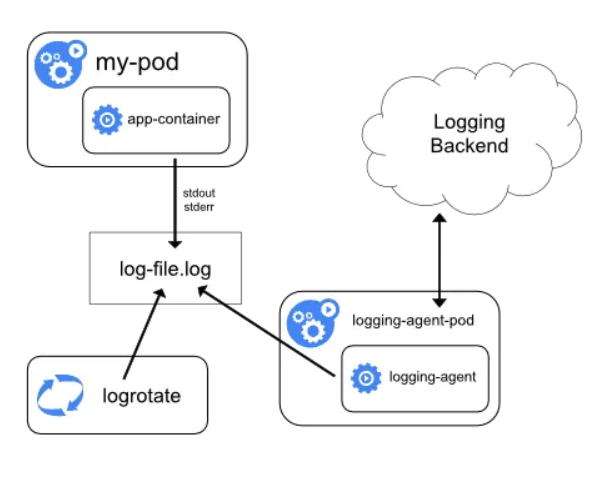
\includegraphics[width=\textwidth]{pictures/loggingsol.png}
\end{figure}

As the logging agent must run on every node, it's common to implement it as either a DaemonSet replica, a manifest pod, or a dedicated native process on the node.

\subsubsection{EFK Solution}

Now that we covered the basics of logging, let's explore EFK solution (ElasticSearch, Fluentd and Kibana). This solution is used by many important companies like: GitHub, Netflix, and Amazon, ITnow XD. It connect Fluentd, ES, and Kibana (as visualization tools) to make an exact namespace with a few services and pods.

\subsubsection{Fluentd (Logs Collector)}
Fluentd is an ideal solution as a unified logging layer. we just have to open and download the type of logger we need for the project.
Fluentd has ready configurations and templates (snippets) to provide simply he setup and customization process when integrating Fluentd with other systems (forwarding the logs in the proper way), such as ElasticSearch (ES), Apache Kafka or Dynatrace.

Fluentd collects logs both from user applications and cluster components such as kube-apiserver and kube-scheduler.
The main advantage of this approach is that data isn’t stored in the JSON file, so it is saved with no exclusions, as well it has timestamps to be able to sort it properly.

There are two different concrete stacks for logging: ELK and EFK. The first is with Elastic domain product, Logstash. However, this tool, which has a lightning connection with ES, doesn’t support k8s directly. This is where the Fluentd open-source project comes in handy

\subsubsection{ElasticSearch + Kibana (Logging Endpoint)}

ElasticSearch (ES) can perform many tasks, all of them centered around searching. ES, developed and provided by Elastic company, is a rapid-fire queryset executor that has impressive data processing and transferring capabilities.

We have choosen Elasticsearch to store, process and extend the logging, monitoring and alerting capabilities. But here I let other available and as well good options:
\begin{itemize}
    \item Prometheus
    \item Apache Kafka
    \item Dynatrace
\end{itemize}

\subsubsection{EFK K8s Resources to Deploy}

\paragraph{EFK: Elasticsearch}
\begin{codetemplate}{}
\begin{verbatim}
apiVersion: apps/v1
kind: Deployment
metadata:
  name: elasticsearch
spec:
  selector:
	matchLabels:
  	component: elasticsearch
  template:
	metadata:
  	labels:
    	component: elasticsearch
	spec:
  	containers:
  	- name: elasticsearch
    	image: docker.elastic.co/elasticsearch/elasticsearch:7.4.1
    	env:
    	- name: discovery.type
      	value: single-node
    	ports:
    	- containerPort: 9200
      	name: http
      	protocol: TCP
    	resources:
      	limits:
        	cpu: 500m
        	memory: 4Gi
      	requests:
        	cpu: 500m
        	memory: 4Gi
\end{verbatim}
\end{codetemplate}

\begin{codetemplate}{}
\begin{verbatim}
apiVersion: v1
kind: Service
metadata:
  name: elasticsearch
  labels:
	service: elasticsearch
spec:
  type: NodePort
  selector:
	component: elasticsearch
  ports:
  - port: 9200
	targetPort: 9200
\end{verbatim}
\end{codetemplate}

\paragraph{EFK: Fluentd}

In order to \textbf{Fluentd} is able to retrieve logs from all the K8s Cluster, we need to create some \textbf{Role-based access control} resources.

\textbf{ServiceAccount:} Fluentd runs as a pod in the Kubernetes cluster and requires a ServiceAccount to authenticate itself when accessing the Kubernetes API to retrieve the necessary log data. So it associates the Pod/fluentd with the specified permissions.

\textbf{ClusterRole:} defines what resources and actions Fluentd is allowed to interact with across the entire Kubernetes cluster: Get, List, and Watch Pods and Namespaces.

\textbf{ClusterRoleBinding:} links the ClusterRole (which defines the permissions) to the ServiceAccount (which identifies the Fluentd pod).

\begin{codetemplate}{}
\begin{verbatim}
apiVersion: v1
kind: ServiceAccount
metadata:
  name: fluentd
  namespace: kube-system
\end{verbatim}
\end{codetemplate}
\begin{codetemplate}{}
\begin{verbatim}
apiVersion: rbac.authorization.k8s.io/v1beta1
kind: ClusterRole
metadata:
  name: fluentd
  namespace: kube-system
rules:
- apiGroups:
  - ""
  resources:
  - pods
  - namespaces
  verbs:
  - get
  - list
  - watch
\end{verbatim}
\end{codetemplate}
\begin{codetemplate}{}
\begin{verbatim}
kind: ClusterRoleBinding
apiVersion: rbac.authorization.k8s.io/v1beta1
metadata:
  name: fluentd
roleRef:
  kind: ClusterRole
  name: fluentd
  apiGroup: rbac.authorization.k8s.io
subjects:
- kind: ServiceAccount
  name: fluentd
  namespace: kube-system
\end{verbatim}
\end{codetemplate}

\begin{codetemplate}{Fluentd\_daemonSet.yaml}
\begin{verbatim}
apiVersion: apps/v1
kind: DaemonSet
metadata:
  name: fluentd
  namespace: kube-system
  labels:
	k8s-app: fluentd-logging
	version: v1
	kubernetes.io/cluster-service: "true"
spec:
  selector:
	matchLabels:
  	k8s-app: fluentd-logging
  template:
	metadata:
  	labels:
    	k8s-app: fluentd-logging
    	version: v1
    	kubernetes.io/cluster-service: "true"
	spec:
  	serviceAccount: fluentd
  	serviceAccountName: fluentd
  	tolerations:
  	- key: node-role.kubernetes.io/master
    	effect: NoSchedule
  	containers:
  	- name: fluentd
    	image: fluent/fluentd-kubernetes-daemonset:v1.3-debian-elasticsearch
    	env:
      	- name:  FLUENT_ELASTICSEARCH_HOST
        	value: "elasticsearch.logging"
      	- name:  FLUENT_ELASTICSEARCH_PORT
        	value: "9200"
      	- name: FLUENT_ELASTICSEARCH_SCHEME
        	value: "http"
      	- name: FLUENT_UID
        	value: "0"
    	resources:
      	limits:
        	memory: 200Mi
      	requests:
        	cpu: 100m
        	memory: 200Mi
    	volumeMounts:
    	- name: varlog
      	  mountPath: /var/log
    	- name: varlibdockercontainers
      	  mountPath: /var/lib/docker/containers
      	  readOnly: true
  	terminationGracePeriodSeconds: 30
  	volumes:
  	- name: varlog
    	hostPath:
      	path: /var/log
  	- name: varlibdockercontainers
    	hostPath:
      	path: /var/lib/docker/containers
\end{verbatim}
\end{codetemplate}

\subsubsection{EFK: Kibana}

Finally, we will use Kibana to make a visual representation of the logs. Create a kibana.yml file with the following lines:

\begin{codetemplate}{}
\begin{verbatim}
apiVersion: apps/v1
kind: Deployment
metadata:
  name: kibana
spec:
  selector:
	matchLabels:
  	run: kibana
  template:
	metadata:
  	labels:
    	run: kibana
	spec:
  	containers:
  	- name: kibana
    	image: docker.elastic.co/kibana/kibana:7.4.1
    	env:
    	- name: ELASTICSEARCH_URL
      	value: http://elasticsearch:9200
    	- name: XPACK_SECURITY_ENABLED
      	value: "true"
    	ports:
    	- containerPort: 5601
      	name: http
      	protocol: TCP
\end{verbatim}
\end{codetemplate}

\begin{codetemplate}{}
\begin{verbatim}
apiVersion: v1
kind: Service
metadata:
  name: kibana
  labels:
	service: kibana
spec:
  type: NodePort
  selector:
	run: kibana
  ports:
  - port: 5601
	targetPort: 5601
\end{verbatim}
\end{codetemplate}

%======================================================
\newpage
\section{Application Lifecycle Management}

\subsection{Rolling Updates \& Rollback}

Before we look at how we upgrade our application, let's try to understand \textbf{rollouts} and \textbf{versioning} in a deployment. When we first create a deployment, it triggers a rollout. A new rollout creates a new deployment revision. In the future, when the app is upgraded, the container version is upgraded to a new one, a new rollout is triggered and a new deployment revision is created. This helps us keep track of the changes made to our deployment and enables us to rollback to a previous version of the deployment if necessary.

See status of a rollout:
\begin{codetemplate}{}
\begin{verbatim}
$ kubectl rollout status <deploy_name>
\end{verbatim}
\end{codetemplate}

See revisions and history of a rollout:
\begin{codetemplate}{}
\begin{verbatim}
$ kubectl rollout history <deploy_name>
\end{verbatim}
\end{codetemplate}

\subsection{Deployment Strategies}

\subsubsection{Recreate Strategy}
Destroy all replicas and then create new ones with the new version of the applications. So at first delete 5 instances and then deploy 5 new ones. The problem with this, as we can imagine, is that during the period after the older versions are down and before any newer version is up, the application is down and inaccessible to users

\subsubsection{Rolling Update}
We do not destroy all of them at once, instead we take down the older version and bring up a newer version one by one. This way, the application never goes down and the upgrade is seamless.

\begin{blocktemplate}{NOTE}
If we not specify the strategy when we create the Deployment, it will assume it to be \textbf{rolling update}, the \textbf{default Deployment strategy}.
\end{blocktemplate}

\begin{figure}[H]
    \centering
    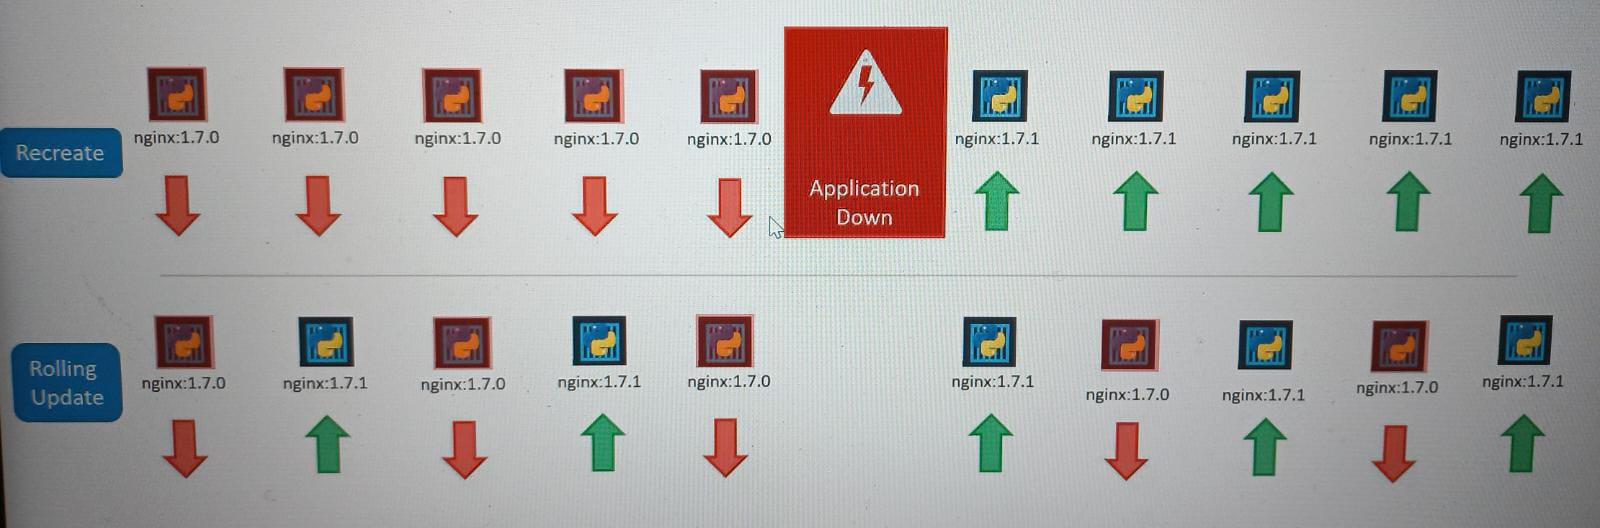
\includegraphics[width=\textwidth]{pictures/depest.png}
\end{figure}

\begin{codetemplate}{}
\begin{verbatim}
apiVersion: apps/v1
kind: Deployment
metadata:
 name: nginx-deployment
 labels:
   app: nginx
spec:
 replicas: 3
 selector:
   matchLabels:
     app: nginx
 template:
   metadata:
     labels:
       app: nginx
   spec:
     containers:
     - name: nginx
       image: nginx:1.14.2
       ports:
       - containerPort: 80
 strategy:
   type: RollingUpdate
   rollingUpdate:
     maxUnavailable: 1
     maxSurge: 1
     #maxUnavailable: 25%
     #maxSurge: 25%
\end{verbatim}
\end{codetemplate}

\begin{blocktemplateI}{NOTE}
Kubernetes doesn't count terminating Pods when calculating the number of availableReplicas, which must be between replicas - maxUnavailable and replicas + maxSurge.
\end{blocktemplateI}

\subsection{How to update a Deployment?}

When we talk about update it can be of so many things: container version, app version, labels, number of replicas, etc. Since we already heave a Deployment definition YAML file, it is easy for us to modify this file. Once we make the necessary changes, we can use:

\begin{codetemplate}{}
\begin{verbatim}
$ kubectl apply -f <deployment-file>.yaml
\end{verbatim}
\end{codetemplate}

So a new rollout is triggered and a new revision  of the deployment is created.

\begin{blocktemplateIII}{WARNING}
If we use \verb|kubectl delete| and then \verb|kubectl create| we are deleting all the replicas so the application will be down at this time and inaccessible to users.
\end{blocktemplateIII}

But there is another way to do the same thing:

\begin{codetemplate}{}
\begin{verbatim}
$ kubectl set image deploy <deploy-name> <container-name>=<image-name>:<tag>
\end{verbatim}
\end{codetemplate}

\begin{codetemplate}{}
\begin{verbatim}
$ kubectl edit deploy <deploy-name>
\end{verbatim}
\end{codetemplate}

\begin{blocktemplateIII}{WARNING}
But remember, doing this will result in the Deployment definition YAML file having a different configuration, so we must be careful if we use the same definition file in the future.
\end{blocktemplateIII}

To see the strategy of a Deployment:
\begin{codetemplate}{}
\begin{verbatim}
$ kubectl describe deploy <deploy-name> | grep -i StrategyType
\end{verbatim}
\end{codetemplate}

\subsection{Deployment updates under the hoods}
When a deployment is created, it creates a new ReplicaSet to create and control the Pods, so if and update is made in the Deployment, it creates a new ReplicaSet and starts deploying the Pods and containers at the same time it is taking down the Pods in the old ReplicaSet following a rolling update strategy.

\subsection{Rollback}
\begin{codetemplate}{}
\begin{verbatim}
$ kubectl rollout undo deploy <deploy-name>
\end{verbatim}
\end{codetemplate}

\subsection{Commands \& Arguments in Pod definition}

\subsubsection{Introduction - Docker CMD \& ENTRYPOINT}

\textbf{CMD}

If we want to run a container from an Ubuntu image, when we run the command \verb|docker run ubuntu| it runs an instance of ubuntu image but immediately dies, if we list the running containers we wouldn't see it running. If we list all the containers we will see that the container is in exited state. But why is that?

Unlike virtual machines, containers are not meant to host an OS (Operating System), \textbf{containers are meant to run a specific task or process}, such as to host an instance of a Web Server, Application Server, Database or simply carry out some computation or analysis. Once the task is complete, the container exits, \textbf{so the container only lives as long as the process inside it is alive}, if the web service inside the container is stopped, or crashes, the container exits. So who defines what process is run within the container? If we look inside popular Docker images like NGINX, we will see that it is specified in its Dockerfile in CMD instruction. So if we look in Ubuntu image, it uses bash as the CMD, and bash is not a real process.

So to specify the command to run inside the container we can do it:

\begin{itemize}
    \item Defining CMD in Dockerfile:
\begin{codetemplate}{Dockerfile}
\begin{verbatim}
CMD ["init-exec.sh"]
\end{verbatim}
\end{codetemplate}

    \item Overwriting the CMD via terminal:
\begin{codetemplate}{}
\begin{verbatim}
$ docker run image init-exec.sh
\end{verbatim}
\end{codetemplate}
\end{itemize}

\textbf{ENTRYPOINT}

The ENTRYPOINT instruction is like CMD instruction, as in, we can specify the program that will be run when the container starts, and whatever we specify on the CMD or un running commands will be appended to ENTRYPOINT. The default ENTRYPOINT is \verb|/bin/bash -c|.

\begin{blocktemplate}{NOTE}
It is not so recomended, but it is possible to overwrite the ENTRYPOINT of an image via commands:
\begin{codetemplate}{}
\begin{verbatim}
$ docker run --entrypoint <entrypoint> <image>:<tag> 
\end{verbatim}
\end{codetemplate}

\end{blocktemplate}

\subsubsection{Commands \& Arguments in a K8s Pod}

The CMD and ENTRYPOINT can be overwritten by K8s in the Pod definition using \verb|args| and \verb|command|:
\begin{itemize}
    \item \verb|args:| overwrite CMD
    \item \verb|command:| overwrite ENTRYPOINT
\end{itemize}
\begin{codetemplate}{}
\begin{verbatim}
...
spec:
    containers:
    - image: ubuntu
      name: ubuntu-container
      command: ["sleep"]
      args:  ["10"]
      ... 
\end{verbatim}
\end{codetemplate}


\begin{blocktemplateII}{NOTE}
Command and args can be defined as well:
\begin{codetemplate}{}
\begin{verbatim}
spec
    ...
    containers:
    - image: ...
      command: 
      - "sleep"
      - "1200"
      args:
      - "c"
      - "while true; do echo hello; done"
\end{verbatim}
\end{codetemplate}
\end{blocktemplateII}

\subsection{Env Vars in Pods}

\subsubsection{Env Vars in Docker Containers}
\begin{codetemplate}{}
\begin{verbatim}
$ docker run -e APP_COLOR=pink nginx
\end{verbatim}
\end{codetemplate}

\subsubsection{Env Vars in Pods Containers with key-values directly}
\begin{codetemplate}{}
\begin{verbatim}
spec:
    containers:
    - image: ...
      env:
      - name: APP_COLOR
        value: pink
\end{verbatim}
\end{codetemplate}

\subsubsection{Env Vars in  Containers using ConfigMaps}
\begin{codetemplate}{}
\begin{verbatim}
spec:
    containers:
    - image: ...
      env:
      - name: APP_COLOR
        valueFrom:
            configMapKeyRef:
                name: <cm_name>     # The ConfigMap this value comes from.
                key: <key>          # The key to fetch.
\end{verbatim}
\end{codetemplate}

\begin{codetemplate}{}
\begin{verbatim}
apiVersion: v1
kind: Pod
spec:
    containers:
    - image: ...
      envFrom:
      - configMapRef:
            name: <cm_name>     # The ConfigMap this value comes from.
\end{verbatim}
\end{codetemplate}

We are going to explain that in more detail in following sections.

\subsubsection{Env Vars in Pods Containers using Secrets}
\begin{codetemplate}{}
\begin{verbatim}
spec:
    containers:
    - image: ...
      env:
      - name: APP_COLOR
        valueFrom:
            secretKeyRef:
\end{verbatim}
\end{codetemplate}

We are going to explain that in more detail in following sections.

\subsection{ConfigMaps}
The way to separate environment variables configuration from Pods definitions to ConfigMaps. They are used to pass configuration data in the form of key value pairs in K8s but out of Pod definition. When the Pod is created we should use the configMapRef to create the env vars inside the container into the Pod.

So there is two phases involved in configuring ConfigMaps:
\begin{enumerate}
    \item ConfigMap Creation
    \item ConfigMap injection into Pods
\end{enumerate}

\subsubsection{ConfigMaps Creation}

\textbf{Imperative Creation}
\begin{codetemplate}{}
\begin{verbatim}
$ kubectl create cm --help
\end{verbatim}
\end{codetemplate}

\begin{codetemplate}{}
\begin{verbatim}
$ kubectl create cm <name> --from-literal=APP_COLOR=blue \
    --from-literal=APP_LETER=mayus \
    --from-literal=...
\end{verbatim}
\end{codetemplate}

\begin{codetemplate}{}
\begin{verbatim}
$ kubectl create cm <name> --from-file=/path/to/file
\end{verbatim}
\end{codetemplate}

\begin{codetemplate}{file.txt}
\begin{verbatim}
APP_COLOR=blue
APP_LETER=mayus
...
\end{verbatim}
\end{codetemplate}

\textbf{Declarative Creation}
\begin{codetemplate}{cm.yaml}
\begin{verbatim}
apiVersion: v1
kind: ConfigMap
metadata:
    name: app-config
data:
    APP_COLOR: blue
    APP_LETER: mayus
\end{verbatim}
\end{codetemplate}
\begin{codetemplate}{}
\begin{verbatim}
$ kubectl create -f cm.yaml
\end{verbatim}
\end{codetemplate}


\subsubsection{ConfigMaps Pod Injection}

\begin{blocktemplateI}{NOTE}
It is common to have so many ConfigMaps for different Pods (fron-end, backend, Database, etc.) for different purposes and configurations, so it is important to name them properly as we will be using these names later while associating it with Pods.
\end{blocktemplateI}

\textbf{As Single Env Var}
\begin{codetemplate}{}
\begin{verbatim}
apiVersion: v1
kind: Pod
spec:
    containers:
    - image: ...
      env:
      - name: APP_COLOR
        valueFrom:
          configMapKeyRef:
            name: <cm_name>     # The ConfigMap this value comes from.
            key: <key>          # The key to fetch.
\end{verbatim}
\end{codetemplate}

\textbf{All variables from ConfigMap}
\begin{codetemplate}{}
\begin{verbatim}
apiVersion: v1
kind: Pod
spec:
    containers:
    - image: ...
      envFrom:
      - configMapRef:
            name: <cm_name>     # The ConfigMap this value comes from.
\end{verbatim}
\end{codetemplate}

\textbf{As File into a Volume}
\begin{codetemplate}{}
\begin{verbatim}
apiVersion: v1
kind: Pod
spec:
    containers:
    - name: <container_name>
      image: ...
      volumeMounts:
      - mountPath: <mount_path>
        name: app-config-volume
    volumes:
    - name: app-config-volume
      configMap:
        name: <cm_name>     # The ConfigMap this value comes from.
\end{verbatim}
\end{codetemplate}

\begin{blocktemplateII}{NOTE}
If we don't configure the ConfigMap as volume, and we just add it to the \verb|env| list, the variable is directly set as variable on the container accessible from shell.
\end{blocktemplateII}

\subsubsection{Pods update when ConfigMaps changes?}
In Kubernetes, Pods don’t automatically restart when the ConfigMap they use is updated. This is because the ConfigMap is mounted as a volume or injected as environment variables, and changes to the ConfigMap itself don't trigger an update event for Pods.

If we want automatic updates of Pods when a ConfigMap changes without a rolling update, we can use the k8s-sidecar container to monitor ConfigMaps and trigger the reload of the application within the Pod.

You would add a sidecar container that watches for changes in the ConfigMap and reloads the application or updates the configuration in real-time.

Here, stakater/reloader or another reloader container can monitor the changes and reload the app inside the pod.

\begin{codetemplate}{}
\begin{verbatim}
apiVersion: apps/v1
kind: Deployment
metadata:
  ...
spec:
  ...
  template:
   ...
    spec:
      containers:
      - name: my-app
        image: my-app-image
        volumeMounts:
        - name: config-volume
          mountPath: /etc/config
        env:
        - name: CONFIG_PATH
          value: "/etc/config/my-config"
      - name: configmap-reloader
        image: stakater/reloader:latest
        env:
        - name: WATCH_NAMESPACE
          valueFrom:
            fieldRef:
              fieldPath: metadata.namespace
        - name: CONFIGMAP_NAME
          value: "my-configmap"
        - name: RESOURCE_TYPE
          value: "deployment"
      volumes:
      - name: config-volume
        configMap:
          name: my-configmap
\end{verbatim}
\end{codetemplate}

\subsection{Secrets}
Store confidential data into ConfigMaps is not a good idea, like passwords or keys, because the value of this objects are clear. There is another type of object similar to ConfigMpas but with data encoded, it is called \textbf{Secret}. As in ConfigMaps there are two steps involved in the creation of a Secret: creation and pod injection.
\subsubsection{Secret Creation}

\textbf{Imperative}
\begin{codetemplate}{}
\begin{verbatim}
$ kubectl create secret generic <secret-name> --from-literal=<key>=<value> \
    --from-literal=<key>-<value>
\end{verbatim}
\end{codetemplate}

\begin{codetemplate}{}
\begin{verbatim}
$ kubectl create secret generic <secret-name> --from-file=<path/to/file>
\end{verbatim}
\end{codetemplate}

\textbf{Declarative}

\begin{codetemplate}{secret.yaml}
\begin{verbatim}
apiVersion: v1
kind: Secret
metadata:
    name: app-secret
data:
    DB_Host: bXlzcWw=
    DB_User: cm9vdA==
    DB_Password: cGFzd3Jk
\end{verbatim}
\end{codetemplate}

\begin{codetemplate}{secret.yaml}
\begin{verbatim}
apiVersion: v1
kind: Secret
metadata:
  name: secret-ssh-auth
type: kubernetes.io/ssh-auth
data:
  ssh-privatekey: |
    UG91cmluZzYlRW1vdGljb24lU2N1YmE=    
\end{verbatim}
\end{codetemplate}

\begin{blocktemplateIII}{WARNING}
Note that the values are encoded (in base64), it is important than when we create Secrets in declarative way, so we should previously encode the values in base64:
\begin{codetemplate}{}
\begin{verbatim}
$ echo -n 'mysql' | base64
\end{verbatim}
\end{codetemplate}
\end{blocktemplateIII}

\subsubsection{Secrets Pod Injection}
\textbf{As a .file inside Container}
\begin{codetemplate}{}
\begin{verbatim}
apiVersion: v1
kind: Secret
metadata:
  name: dotfile-secret
data:
  .secret-file: dmFsdWUtMg0KDQo=
\end{verbatim}
\end{codetemplate}
\begin{codetemplate}{}
\begin{verbatim}
apiVersion: v1
kind: Pod
metadata:
  name: secret-dotfiles-pod
spec:
  volumes:
    - name: secret-volume
      secret:
        secretName: dotfile-secret
  containers:
    - name: dotfile-test-container
      image: registry.k8s.io/busybox
      command:
        - ls
        - "-l"
        - "/etc/secret-volume"
      volumeMounts:
        - name: secret-volume
          readOnly: true
          mountPath: "/etc/secret-volume"
\end{verbatim}
\end{codetemplate}

\textbf{As Single Env Vars}
\begin{codetemplate}{}
\begin{verbatim}
apiVersion: v1
kind: Secret
metadata:
  name: app-secret
data:
  DB_Password: bXlzcWw=
\end{verbatim}
\end{codetemplate}
\begin{codetemplate}{}
\begin{verbatim}
apiVersion: v1
kind: Pod
metadata:
    name: secret-pod
    labels:
        name: secret-pod
spec:
    containers:
    - name: simple-webapp-color
      image: simple-webapp-color
      env:
      - name: DB_Pawd
        valueFrom:
            secretKeyRef:
                name: app-secret
                key: DB_Password
      ...
\end{verbatim}
\end{codetemplate}

\textbf{All env vars from Secret}
\begin{codetemplate}{}
\begin{verbatim}
apiVersion: v1
kind: Secret
metadata:
  name: app-secret
data:
  DB_User: root
  DB_Password: bXlzcWw=
  DB_connection_string: mysql.connection.string 
\end{verbatim}
\end{codetemplate}
\begin{codetemplate}{}
\begin{verbatim}
apiVersion: v1
kind: Pod
metadata:
    name: secret-pod
    labels:
        name: secret-pod
spec:
    containers:
    - name: simple-webapp-color
      image: simple-webapp-color
      envFrom:                                                                                                                                            
      - secretRef:                                                                                                                                        
          name: db-secret
    ...
    ...
        volumeMount:
    ...
    volumes:
    - name: app-secret-volume
      secret:
        secretName: app-secret
      ...
        volumeMount:
    ...
    volumes:
    - name: app-secret-volume
      secret:
        secretName: app-secret
\end{verbatim}
\end{codetemplate}

\subsubsection{View Secrets}
\begin{codetemplate}{}
\begin{verbatim}
$ kubectl get secrets
\end{verbatim}
\end{codetemplate}
\begin{blocktemplateIII}{WARNING}
Note that the values are encoded (in base64), so to retrieve them we have to decode them in base64.
\begin{codetemplate}{}
\begin{verbatim}
$ echo -n 'bXlzcWw=' | base64 -d
\end{verbatim}
\end{codetemplate}
\end{blocktemplateIII}

\subsubsection{Secrets Notes}
\begin{itemize}
    \item Secrets are encoded not encrypted, meaning anyone can look up the file that we created for secrets or get the secret object and then decode it in base64 as we did. So it is recommended to not put secret definition inside the git code repositories, because it can be easily retrieved.
    \item Remember that some that can access to Deployments or Pods in a Namespace can also access to Secrets. So we should consider to configure a role-based access control to restrict access (RBAC).
    \item Secrets are not encoded in etcd, so none of the data is encrypted or coded in etcd by default. So we can check this document about encrypting secret data at rest: \href{https://pwittrock.github.io/docs/tasks/administer-cluster/encrypt-data/}{Encrypting Secret Data at Rest}
    \item There are other better ways of handling sensitive data like passwords in Kubernetes, such as using tools like:
    \begin{itemize}
        \item AWS Provider
        \item Azure Provider
        \item HashiCorp Vault
        \item Helm Secrets
        \item GCP Provider
        \item ...
    \end{itemize}
\end{itemize}

There are different type of secrets, for more information check the \href{https://kubernetes.io/docs/concepts/configuration/secret/}{Official Doc}

\subsection{Multi Container Pods}
The idea of decoupling a large monolithic application into sub-components known as \textbf{microservices} enables us to develop and deploy a set of independent, small and reusable code. This architecture helps us to scale every service as required, as opposed to modifying the entire application.. 

But in some case, we will need some instances or service run together to reuse code and scale up and down together, with the same access to Volumes, Secrets, Network... For that purpose we can define multiple containers in a Pod, but this is not usual.

\begin{codetemplate}{}
\begin{verbatim}
apiVersion: v1
kind: Pod
metadata:
    name: simple-webapp
    labels:
        name: simple-webapp
spec:
    containers:
    - name: simple-webapp
      image: simple-webapp
      ports:
      - containerPort: 8080
    - name: log-agent
      image: log-agent
    - name: istio-proxy
      image: istio-envoy
\end{verbatim}
\end{codetemplate}

You can retrieve logs for a specific container:
\begin{codetemplate}{}
\begin{verbatim}
$ kubectl logs <pod_name> -c <container_name>
\end{verbatim}
\end{codetemplate}

You can access via shell the specific container:
\begin{codetemplate}{}
\begin{verbatim}
$ kubectl exec -it <pod_name> -c <container_name> -- <command_to_exec>
\end{verbatim}
\end{codetemplate}

\subsection{Init Containers}
In a multi-container pod, each container is expected to run a process that stays alive as long as the POD's lifecycle. But at times we may want to run a process that runs to completion in a container. For example a process that pulls a code or binary from a repository that will be used by the main web application. That is a task that will be run only  one time when the pod is first created. Or a process that waits  for an external service or database to be up before the actual application starts. That's where initContainers comes in.

An initContainer is configured in a pod like all other containers, except that it is specified inside a initContainers section,  like this:

\begin{codetemplate}{}
\begin{verbatim}
apiVersion: v1
kind: Pod
metadata:
  name: myapp-pod
  labels:
    app: myapp
spec:
  containers:
  - name: myapp-container
    image: busybox:1.28
    command: ['sh', '-c', 'echo The app is running! && sleep 3600']
  initContainers:
  - name: init-myservice
    image: busybox
    command: ['sh', '-c', 
        'git clone <some-repository-that-will-be-used-by-application> ; done;']
\end{verbatim}
\end{codetemplate}

When a POD is first created the initContainer is run, and the process in the initContainer must run to a completion before the real container hosting the application starts. 

You can configure multiple such initContainers as well, like how we did for multi-containers pod. In that case each init container is run one at a time in sequential order. If any of the initContainers fail to complete, Kubernetes restarts the Pod repeatedly until the Init Container succeeds.

You can retrieve logs for a specific container:
\begin{codetemplate}{}
\begin{verbatim}
$ kubectl logs <pod_name> -c <container_name>
\end{verbatim}
\end{codetemplate}

\begin{blocktemplateII}{NOTE}
As well, we can access via shell the specific container,
but we should do it when the initcontainer is still running (to debug we can add as command some sleep):
\begin{codetemplate}{}
\begin{verbatim}
$ kubectl exec -it <pod_name> -c <container_name> -- <command_to_exec>
\end{verbatim}
\end{codetemplate}
\end{blocktemplateII}

\subsection{Self Healing Applications}

Kubernetes supports self-healing applications through ReplicaSets and Replication Controllers. The replication controller helps in ensuring that a POD is re-created automatically when the application within the POD crashes. It helps in ensuring enough replicas of the application are running at all times.

Kubernetes provides additional support to check the health of applications running within PODs and take necessary actions through Liveness and Readiness Probes. However these are not required for the CKA exam and as such they are not covered here. These are topics for the Certified Kubernetes Application Developers (CKAD) exam and are covered in the CKAD course.

\section{Cluster Mantaince}

\subsection{Upgrades}
Scenarios where we might have to take down nodes as part of we cluster, say for maintenance purposes, like upgrading a based software or applying patches, security patches, etc.

\subsubsection{What happens when a Node goes down?} 
If the Node comes back online immediately, then the kubelet process starts and the Pods come back online. 

But if the Node does not come back for more than 5 minutes, then the Pods running on that Node are terminated and K8s consider them as dead. And if the Pods are part of a replicaSet then they will be recreated into another Node.

This time of 5 minutes is called \textbf{pod-eviction-timeout} and it is configured in the \textbf{kube-controller-manager} by default as 5 minutes.

If the Node comes back after pod-eviction-timeout it comes up blank, without any pod scheduled on it.

\subsubsection{Node drain}

As we can imagine, if we know that a Node will be unavailable for some time, there is a safer way to do it without danger, purposelly drain the node of all the Workloads running on it:

At first, we should tell K8s to not schedule more Pods on the Node, because we are going to take actions on it:
\begin{codetemplate}{}
\begin{verbatim}
$ kubectl cordon <node-name>
\end{verbatim}
\end{codetemplate}

Then, we should move all the Pods running on the node into another Nodes in the Cluster. This means that Pods are terminated from the node they were running and recreated into another Node.
\begin{codetemplate}{}
\begin{verbatim}
$ kubectl drain <node-name>
\end{verbatim}
\end{codetemplate}

When we have finished with the maintaince actions, we should make the Node schedulable again:
\begin{codetemplate}{}
\begin{verbatim}
$ kubectl uncordon <node-name>
\end{verbatim}
\end{codetemplate}

\begin{blocktemplateIII}{WARNING}
A Node cannot be drained if there are Pods running without a ReplicaSet or ReplicationController. It is logic, because without these objects the Pod will be lost forever.
\\\\
But we can force it:
\begin{codetemplate}{}
\begin{verbatim}
$ kubectl drain --force <node_name>
\end{verbatim}
\end{codetemplate}
As well, nodes running \textbf{daemonSets} cannot be normally drained, so we can use force as well to remove the pods or \verb|--ignore-daemonsets| to do not drain them:
\begin{codetemplate}{}
\begin{verbatim}
$ kubectl drain --ignore-daemonsets <node_name>
\end{verbatim}
\end{codetemplate}
\end{blocktemplateIII}

\subsection{Cluster Upgrade Process}

\subsubsection{K8s Releases}
When we install a K8s Cluster, we install a specific version of K8s, we can see the version running on the nodes:

\begin{codetemplate}{}
\begin{verbatim}
$ kc get nodes
\end{verbatim}
\end{codetemplate}

Let's see for example \textbf{v1.11.3}, it consists of three parts (MAJOR, MINOR \& PATCH). All the releases we can see here are stable releases. Also we can also see alpha and beta releases called: \textbf{v1.x.x-alpha} or \textbf{v1.x.x-beta} if it is in a more mature stage.

You can check K8s versions: \href{https://github.com/kubernetes/kubernetes}{https://github.com/kubernetes/kubernetes}

\subsubsection{Cluster Upgrade Process}

The different components can be at different release versons, 
since the kube-apiserver is the primary component in the control plane, 
and this is the components that all other components talk to, \textbf{none of the other components can be at a version higher than the kube-apiserver}. The \textbf{controller-manager} and \textbf{scheduler} can be at most one version lower. And \textbf{kubelet} and \textbf{kubeproxy} can be at most 2 versions lower. The kubectl version could be at most 1 superior or 1 lower.

\begin{figure}[H]
    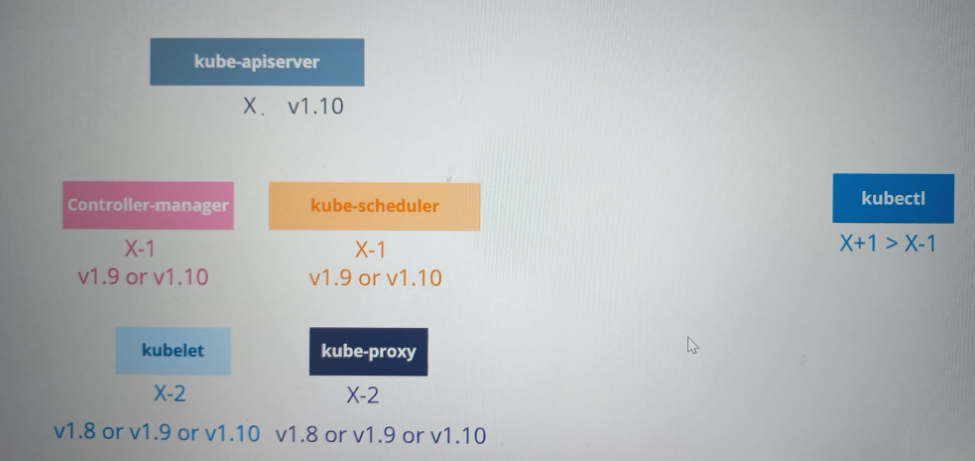
\includegraphics[scale=0.5]{pictures/clusup.png}
\end{figure}

\textbf{K8s Support}
The images supported by K8s are always the last three MINOR version release. But it is not recommended to upgrade 3 versions at time, it is better to upgrade step by stpe, by 1 version in 1 version.

\begin{figure}[H]
    \includegraphics[scale=0.13]{pictures/clusup1.png}
\end{figure}

\paragraph{kubeadm Upgrade Plan}

Imagine we have a cluster with Master and Worker Nodes, with applications running in production, hosting Pods, serving users. At first they are upgraded the Master Nodes (control-plane Nodes) version and then the Worker Nodes versions. When Master Nodes (control-plane Nodes) goes down does not mean our Worker Nodes and applications on the Cluster are impacted. All workloads hosted on the Worker Nodes continue to serve users as normal, but all the management functions are down, so we cannot access the cluster using kubectl or other K8s API, so we cannot deploy new applications or modify existing ones.  But deployments and ReplicaSets are already running, so if a Pod fails, it is automatically deployed.

Once the Master Nodes (control-plane Nodes) are Upgraded, now it is time to upgrade Worker Nodes, there are different strategies to update Worker Nodes, one is update all of them at once, but this is not recommended, because all Pods are down and users are no longer able to access the applications. Once the update is completed, new Pods are scheduled and users can resume access.

The seconds strategy, the one recommended is to update one Node as a time, so when we update one node, the Pods that were running on it are automatically re-scheduled into another Nodes. So when a Node is upgraded, then the next one is updated and so on until the end.

\begin{codetemplate}{}
\begin{verbatim}
$ kubeadm upgrade plan
\end{verbatim}
\end{codetemplate}

With this command we can see the version of all components in the K8s Cluster. Also we can see the version which they can be updated. Finally it says that once we have upgrade the K8s components, we have to upgrade manually the kubelet on each Node.

\paragraph{Steps to upgrade K8s version from 1.11 to 1.13}

\begin{enumerate}

    \item Update the system to have the latest versions of the binaries and services:
\begin{codetemplate}{}
\begin{verbatim}
$ sudo apt-get update
\end{verbatim}
\end{codetemplate}

    \item Check the \verb|kubeadm| version we want is available for our system:
\begin{codetemplate}{}
\begin{verbatim}
$ sudo apt-cache madison kubeadm
\end{verbatim}
\end{codetemplate}

    \item Upgrade the \verb|kubeadm| version to version 1.12
\begin{codetemplate}{}
\begin{verbatim}
$ sudo apt-get upgrade -y kubeadm=1.12.0-00
\end{verbatim}
\end{codetemplate}

    \item Upgrade the Cluster
\begin{codetemplate}{}
\begin{verbatim}
$ kubeadm upgrade plan
\end{verbatim}
\end{codetemplate}
\begin{codetemplate}{}
\begin{verbatim}
$ kubeadm upgrade apply v1.12.0 -y
\end{verbatim}
\end{codetemplate}

    \item Get Nodes to see the Nodes version, it will still be in 1.11, because this command shows the version of the kubelets.
\begin{codetemplate}{}
\begin{verbatim}
$ kubectl get nodes
\end{verbatim}
\end{codetemplate}

    \item Go to the Master Nodes (control-plane Nodes) and update the system:
\begin{codetemplate}{}
\begin{verbatim}
$ sudo apt-get update
\end{verbatim}
\end{codetemplate}

    \item Check on the Master Node (control-plane Node)that the version we want to install is available:
\begin{codetemplate}{}
\begin{verbatim}
$ sudo apt-cache madison kubelet
\end{verbatim}
\end{codetemplate}

    \item Upgrade kubelet version:
\begin{codetemplate}{}
\begin{verbatim}
$ sudo apt-get upgrade -y kubelet=1.12.0-00
\end{verbatim}
\end{codetemplate}
\begin{codetemplate}{}
\begin{verbatim}
$ systemctl restart kubelet
\end{verbatim}
\end{codetemplate}

    \item Cordon the first Worker Node we want to upgrade:
\begin{codetemplate}{}
\begin{verbatim}
$ kubectl cordon node-1
\end{verbatim}
\end{codetemplate}

    \item Drain Pods from this Worker Node:
\begin{codetemplate}{}
\begin{verbatim}
$ kubectl drain node-1
\end{verbatim}
\end{codetemplate}

    \item Go to the Worker Node and upgrade the \verb|kubeadm| version
\begin{codetemplate}{}
\begin{verbatim}
$ sudo apt-get upgrade -y kubeadm=1.12.0-00
\end{verbatim}
\end{codetemplate}

    \item Now install and download the kubelet version:
\begin{codetemplate}{}
\begin{verbatim}
$ apt install kubelet=1.12.0-00 -y
\end{verbatim}
\end{codetemplate}
\begin{codetemplate}{}
\begin{verbatim}
$ sudo apt-get upgrade -y kubelet=1.12.0-00
\end{verbatim}
\end{codetemplate}
\begin{codetemplate}{}
\begin{verbatim}
$ kubeadm upgrade node config --kubelet-version v1.12.0
\end{verbatim}
\end{codetemplate}
\begin{codetemplate}{}
\begin{verbatim}
$ systemctl restart kubelet
\end{verbatim}
\end{codetemplate}
\begin{codetemplate}{}
\begin{verbatim}
$ kubectl uncordon node-1
\end{verbatim}
\end{codetemplate}

    \item Do the same for the rest of the Worker Nodes
\end{enumerate}

\begin{figure}[H]
    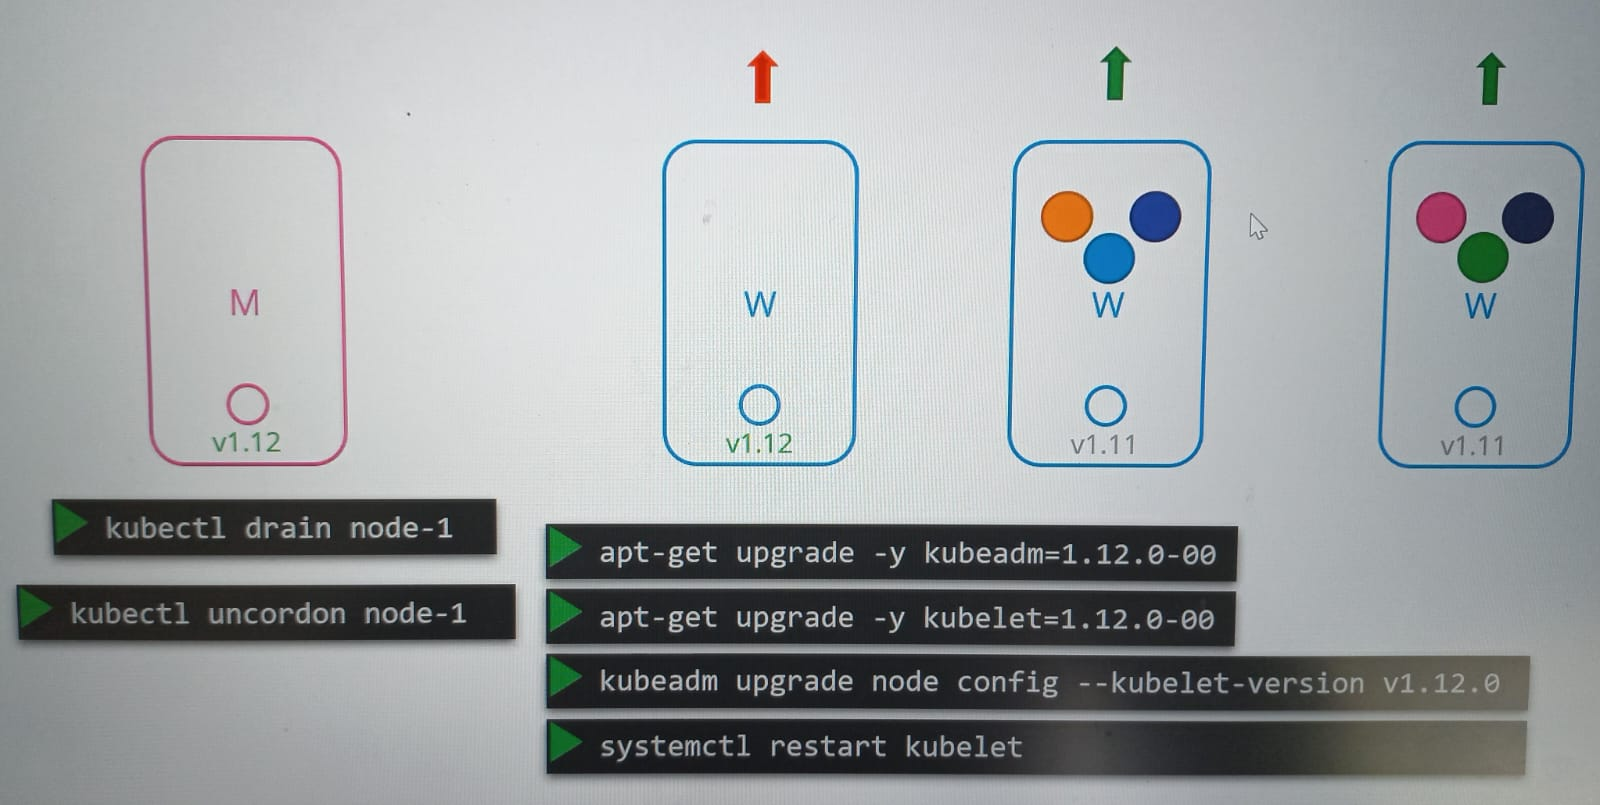
\includegraphics[width=\textwidth]{pictures/clusup2.png}
\end{figure}

\begin{blocktemplateIII}{WARNING}
If kubeadm or kubelet are not installed in the Node, at first it is needed to install them:
\begin{codetemplate}{}
\begin{verbatim}
$ sudo apt install kubelet=1.27.0-00
\end{verbatim}
\end{codetemplate}
\end{blocktemplateIII}

\begin{blocktemplateII}{NOTE}
If we are a cluster admin, and we need to access different nodes, we can use SSH to connect to them via their internal ip:
\begin{codetemplate}{}
\begin{verbatim}
$ kubectl get nodes -o wide
\end{verbatim}
\end{codetemplate}
\end{blocktemplateII}

\begin{blocktemplateI}{NOTE}
To know easily the IP of a Pod or the Node where it is running, we can use the following command:
\begin{codetemplate}{}
\begin{verbatim}
$ kubectl get po -o wide
\end{verbatim}
\end{codetemplate}
\end{blocktemplateI}

\subsection{Backup and Restore Methods}
\subsubsection{Resources}
In resources, the best way to ensure backups is based on 2 concepts:
\begin{itemize}
    \item Use always \verb|kubectl apply| instead of \verb|kubectl create| or \verb|kubectl run|. If we need the template, we can always do:
\begin{codetemplate}{}
\begin{verbatim}
$ kubectl create deploy my-deployment --image=nginx --replicas=3 \
    --dry-run="client" -o yaml > deployment.yaml
\end{verbatim}
\end{codetemplate}
\begin{codetemplate}{}
\begin{verbatim}
$ kubectl apply -f deployment.yaml
\end{verbatim}
\end{codetemplate}

    \item Always store the resources files into a git repository, mantaining them always updated. And enabling we to recover backups if needed.
\end{itemize}

With this configuration, even if we lose our entire cluster, we will be able to recover the applications using the templates (YAML), however we will lose all our data.

You can retrieve logs for a specific container:
\begin{codetemplate}{}
\begin{verbatim}
$ kubectl logs <pod_name> -c <container_name>
\end{verbatim}
\end{codetemplate}

\begin{blocktemplateII}{NOTE}
If Pods has been created in imperative way, the best approach is then:
\begin{itemize}
    \item Recover all the resources created on the cluster:
\begin{codetemplate}{}
\begin{verbatim}
$ kubectl get all -A -o yaml > all_resources.yaml
\end{verbatim}
\end{codetemplate}

    \item Store it into a git repo.
\end{itemize}
\end{blocktemplateII}

\subsubsection{ETCD}
\textbf{Etcd} which is running on all Master Nodes (control-plane Nodes) enables the option of take and recover snapshots. For more information check \href{https://kubernetes.io/docs/tasks/administer-cluster/configure-upgrade-etcd/}{The Official Documentation}

%==========================================================
\newpage
\section{Security}

Security in K8s cluster is related to how access to the K8s Cluster is managed (authentication) and how are the actions controlled inside it.


\subsection{Security in K8s Introduction}
The first security that we should take into account inside a K8s Cluster is the security of the Nodes itself. The bast practices say:
\begin{itemize}
    \item Route access disabled
    \item PasswordAuthentication disabled
    \item Just SSH key authentication enabled
\end{itemize}

But, our focus on this section is more on the K8s related security. As we have seen \textbf{kube-apiserver} is at the center
of all operations within K8s, we interact with it using \verb|kubectl| or by accessing the API directly. With that, we can almost perform any operation inside the cluster. So this should be the first line of defense, controlling the access to \textbf{kube-apiserver} itself.

Who can access? K8s has different methods of authentication:
\begin{itemize}
    \item Username and passwords stored in static files.
    \item Username and tokens stored in static files.
    \item Certificates.
    \item External Authentication providers like LDAP.
    \item Service Accounts (for machines and K8s resources).
\end{itemize}

What they can do? K8s has different methods of control that, but the most used is \textbf{RBAC Authorization (Role-Based Access Control)}, where users are associated to groups with specific permissions.

All the communication inside the cluster can be secured using TLS encryption.

However, by default, all pods can access al other pods within the cluster, but we can restric them using \textbf{network policies}

\subsection{Authentication and Authorization, who can access the cluster?}

To a K8s there are a lot of entities that want to access for different purposes:
\begin{itemize}
    \item \textbf{Administrators:} to administrate the cluster.
    \item \textbf{DevOps:} to check all the objects they deploy are running properly.
    \item \textbf{Developers:} to check the applications are running properly.
    \item \textbf{End Users:} which are going to use the application. Actually it is not managed by the K8s cluster, it is managed by the application itself.
    \item \textbf{External Tools:} which connects to the cluster to retrieve data or trigger actions.
\end{itemize}

K8s does not manage user accounts natively, it relies on an external source like a file with user details or certificates or a third party identity service like LDA to manage the authentication. So, we cannot directly create users into a K8s Cluster.

The only thing related to Authentication and Authorization that K8s can manage is \textbf{ServiceAccounts}. All user Authentication and Authorization is managed by the API server (kube-apiserver). So, how does the \textbf{kube-apiserver} authenticates? There are different methods:

\begin{itemize}
    \item List of usernames and passwords on an static file.
    \item List of usernames and tokens on an static file.
    \item Certificates.
    \item LDAP.
\end{itemize}

Let's start with \textbf{Static Files}.

\subsubsection{Static File Authentication}
A list of users and their passwords or tokens can be created in a CSV file and use it as the source for user information.
The file should have 4 columns: password or token, username, userid, group.

It should be configured on the \textbf{kube-apiserver} service or pod (depending how are we running our cluster) with:
\begin{codetemplate}{}
\begin{verbatim}
--basic-auth-file=user-details.csv
\end{verbatim}
\end{codetemplate}

Or if we want tokens:
\begin{codetemplate}{}
\begin{verbatim}
--token-auth-file=user-details.csv
\end{verbatim}
\end{codetemplate}

To authenticate using static files, we should:
\begin{codetemplate}{}
\begin{verbatim}
$ curl -vk https://<master-node-ip>:6443/api/v1/pods -u "user1:password123"
\end{verbatim}
\end{codetemplate}

To authenticate using static files, we should:
\begin{codetemplate}{}
\begin{verbatim}
$ curl -vk https://<master-node-ip>:6443/api/v1/pods \
    --header "Authorization: Bearer fafhflafhsash..."
\end{verbatim}
\end{codetemplate}

\begin{blocktemplateIII}{WARNING}
This is not the recommended authentication and authorization mechanism, as it is not much sercure.
\end{blocktemplateIII}

\subsection{TLS Introduction (not for K8s)}

\subsubsection{Why do we need certificates?}
Certificates are used to guarantee trust between 2 parties during a transaction. For example: when a user is trying to access a web server, TLS certificates ensure that the communication between the user and the server it is encrypted and they are both who they sey they are (there is no man in the middle).

The data between communications are encrypted using asymetric keys, so only the receiver of the data can decrypt the data, even the sender cannot decrypt the message once it has been sent. A good example to understan asymetric encryption is to think like:
\begin{itemize}
    \item \textbf{Public Key:} Lock that anyone can try to open.
    \item \textbf{Private Key:} The only key which can open the lock, never should be shared.
\end{itemize}

All the times you're requested for connection we are sharing our public key, 
so it is really public XD. Here is the "key" XD: public and private key are related each other,
the sender encrypts the message using his own private key and the public key of the server. And then the server is able to
decrypt it using his private key, all thanks to the relation between pubkey and privkey. 

So the man in the middle is dead, because he does not have any of the private keys and he does not know the relation between public keys and private keys. In summary, he cannot decrypt the message.

So the only chance the man in the middle has, is to recreate the exact website and tell you: hey, I'm our bank, send me our credentials! So the website has its own public and private keys and it starts the negotiation with you. So if we answer, we are dead.

But what if we could know in advance if the pubkey of the server is a legitimate key from our real bank server?
So that's what certificates exactly do! When we are connecting through \textbf{https}, our bank account is sending we a \textbf{Certificate} instead of the pubkey.
This certificate (among other things) has the pubkey inside. Inside the certificate there is information as:
\begin{itemize}
    \item CN (Common Name): domain it is certifying.
    \item Identity: individual, organization, or device
    \item Location: country, state, localty.
    \item PubKey.
    \item Signature.
    \item Signature Algorithm.
    \item Validity Period.
\end{itemize}

But, anyone can create its own certificate, so for that, the browsers check the certificates are signed by a \textbf{(CA) Certificate Authority} which recognizes that 
the certificate is legitime and it is used to certify the domain it is saying. CA's can sign and validate the certificates, the most popular are: DigiCert, Symantec, Comodo, GlobalSign.

How all of them works?

\begin{enumerate}
    \item we generate a \textbf{CSR:} Certificate Signing Request with our domain.
\begin{codetemplate}{}
\begin{verbatim}
$ openssl req -new -key my-bank.key -out my-bank.csr \
    -subj "C=US/ST=CA/O=MyOrg, Inc./CN=mydomain.com"
\end{verbatim}
\end{codetemplate}
    \item The CSR should be sent to the \textbf{CA} for signing.
    \item The CA verify our details and once it checks out, they sign the certificate and send it back to you.
    \item we now have a certificate signed by a CA which the Browsers trust.
\end{enumerate}

\begin{blocktemplateI}{Note}
How Browsers know that the CA which signed the certificate is trustable? Because CA's generate the certificate using it's own pair keys, so the public keys of all the legitimate CAs are built
into all the browsers. Then the browsers use the public key of the CA to validate that the certificate
is actually signed by a legitimate CA.
\end{blocktemplateI}

As well, we can use \textbf{certbot (let's encrypt)} (like a CA), but more quicklier and easier to do, take a look on \href{https://certbot.eff.org/}{CertBot Official Documentation}.

Once our browser and we trust in the server, we can send our sensitive data which will be encrypted using the asymetric key encryption method, and only and actually just only the receiver can decrypt.

\begin{blocktemplateI}{Note}
In some cases, servers can also request a client certificate to authenticate the user or device connecting to them, verifying they are who they say they are. we can not send them, then the server will decide what to share or not share with you.
\\\\
However, our operating system or device (Windows, macOS, Linux, or even a smartphone) manages the whole process for we behind the scenes; our operating system comes with a built-in set of trusted root certificates from trusted certificate authorities (CAs) like DigiCert, Let's Encrypt, etc. These CAs issue certificates to servers (like the one hosting ChatGPT).
\end{blocktemplateI}

Certificates including public keys are stored always with this two extensions: 
\begin{itemize}
    \item \textbf{.pem}: server.pem
    \item \textbf{.crt}: server.crt
\end{itemize}

The private key needed to decrypt messages are stored always with this extension \textbf{.key}: server.key

\begin{blocktemplateI}{Note}
As the key pairs are related, we can encrypt using both of them. So if we encrypt with one of them, we only can decrypt with the other.
\\\\
But take care, the common use is to encrypt with our public key and the public key of the receiver to just the receiver can decrypt using its private key. But if we encrypt using our privatekey, we message will be opened to the world because it can be decrypted with our pubkey.
\end{blocktemplateI}

All the infraestructure regarding this is called \textbf{PKI (Public Key Infraestructure)}, which contains:
\begin{itemize}
    \item Certificates
    \item Certificate Signing Request
    \item CA'S
    \item PubKey and PrivKey
    \item ...
\end{itemize}

So with all of this we have 3 types of certificates based on where they are:
\begin{itemize}
    \item \textbf{Server Certificates:} the ones configured on the servers side.
    \item \textbf{Root Certificate:} configured on the CA servers.
    \item \textbf{Client Certificates:} the ones configured on the clients side. 
\end{itemize}

So in order to know properly which one is server, client... I recommend to name them properly:
\begin{itemize}
    \item server.pem / server.crt / server.key 
    \item client.pem / client.crt / client.key
\end{itemize}
\subsection{Introduction to TLS on K8s}
A K8s Cluster consists of a set of Master and Worker nodes, of course with constant communication between them. So, all the communications inside a K8s Cluster must be secured, so should be encrypted.
For example an administrator using \verb|kubectl| to interact with cluster must establish sceure TLS connection as well as communications between all the components within a K8s Cluster.

To accomplish that, all the clients and servers in a K8s Cluster should have their client certificate and privkey and their server certificate and privkey, to ensure they are who they say they are.

So let's identify the different servers and clients we have within a K8s Cluster.

\textbf{Kube-apiserver} exposes an HTTPS service that other components as well as external users can connect to manage the K8s Cluster. So it is a \textbf{server}, so it must have its server certificate and privkey. But it is a client as well, because it 
needs to communicate with etcd and kubelet, so it can use just the same pair of cert-key for server and client or it can use two pair cert-key; one for server an other for client:
\begin{itemize}
    \item apiserver.crt
    \item apiserver.key
\end{itemize}

\textbf{Etcd} stores all information about the cluster, so it requires as well its certificate and privkey:
\begin{itemize}
    \item etcdserver.crt
    \item etcdserver.key
\end{itemize}

\textbf{Kubelet} exposes and HTTPS API endpoint which the kube-apiserver talks to interact with the Worker Nodes, so:
\begin{itemize}
    \item kubelet.crt
    \item kubelet.key
\end{itemize}

\textbf{Kube-scheduler} is a client of the kube-apiserver, telling which pods need to be deployed on which node, so:
\begin{itemize}
    \item scheduler.crt
    \item shceduler.key
\end{itemize}

\textbf{User accessing kubectl} is a client, so we need as well our client certificate and privkey
to authenticate to the kube-apiserver:
\begin{itemize}
    \item admin.crt
    \item admin.key
\end{itemize}

As well \textbf{kube-controller-manager} and \textbf{kube-proxy} are kube-apiserver clients, so they need their certificates and privkeys:
\begin{itemize}
    \item controller-manager.crt
    \item controller-manager.key
    \item kube-proxy.crt
    \item kube-proxy.key
\end{itemize}

K8s at least one CA (Certificate Authority) for our cluster, to sign all these certificates. In fact, we can have more than one. The CA's have their own pair or cert-key:
\begin{itemize}
    \item CA.crt
    \item CA.key
\end{itemize}

\subsection{Certificate Creation for K8s}
For generating certificates there are different tools available such as:
\begin{itemize}
    \item \verb|openssl|
    \item \verb|easyrsa|
    \item \verb|cfssl|
    \item ...
\end{itemize}

We are going to use the \verb|openssl| tool to generate the certificates.

\subsubsection{Generating CA Certificate}

\begin{enumerate}
    \item Create the \textbf{CA} private key:
\begin{codetemplate}{}
\begin{verbatim}
$ openssl genrsa -out ca.key 2048
\end{verbatim}
\end{codetemplate}

    \item Request a CSR (Certificate Signing Request) for the \textbf{CA} along with the key we've just created:
\begin{codetemplate}{}
\begin{verbatim}
$ openssl req -new ca.key -subj "/CN=KUBERNETES-CA" -out ca.csr
\end{verbatim}
\end{codetemplate}
\begin{blocktemplateI}{Note}
A CSR (Certificate Signing Request) will be like a normal certificate, 
with same information, but without the signature. When we create a CSR, 
we should specify the CN, which will be the name of the component the certificate is for.
\end{blocktemplateI}
    \item Self-sign the certificate:
\begin{codetemplate}{}
\begin{verbatim}
$ openssl x509 -req -in ca.csr -signkey ca.key -out ca.crt
\end{verbatim}
\end{codetemplate}
\begin{blocktemplate}{Note}
As this certificate will be for the CA itself, it will be self-signed. For the rest of the generated
certificates, they are going to be signed with the CA certificate-privkay pairs.
\end{blocktemplate}
\end{enumerate}

\subsubsection{Generating Client Certificates}

\paragraph{Admin User Certificate}

\begin{enumerate}
    \item Create the Admin User private key:
\begin{codetemplate}{}
\begin{verbatim}
$ openssl genrsa -out admin.key 2048
\end{verbatim}
\end{codetemplate}

    \item Request a CSR for the Admin User along with the key we've just created:
\begin{codetemplate}{}
\begin{verbatim}
$ openssl req -new admin.key -subj "/CN=kube-admin/O=system:masters" \
    -out admin.csr
\end{verbatim}
\end{codetemplate}
\begin{blocktemplateI}{Note}
The system:masters label into the CN is added to differentiate admin permissions from general permissions. To make it work, a group named system:masters should exist on K8s with administrative privileges.
\end{blocktemplateI}

    \item Sign the certificate with the CA certificate and CA privkey, to make the certificate valid within the Cluster:
\begin{codetemplate}{}
\begin{verbatim}
$ openssl x509 -req -in admin.csr -CA ca.crt -CAkey ca.key -out admin.crt
\end{verbatim}
\end{codetemplate}
\end{enumerate}

This \verb|admin.crt| will be the Certificate that admin users are going to use to authenticate into K8s Cluster.

\paragraph{How to use Admin User certificate}

\textbf{Not used way}
\begin{codetemplate}{}
\begin{verbatim}
$ curl https://kube-apiserver:6443/api/v1/pods \
    --key admin.key --cert admin.crt \
    --cacert ca.crt
\end{verbatim}
\end{codetemplate}

\textbf{Used way - Kubeconfig file}
\begin{codetemplate}{~/.kube/config}
\begin{verbatim}
apiVersion: v1
clusters:
- cluster:
    certificate-authority: TST_ca.crt
    server: https://<HA_TST_Proxy>:6443
  name: TST_cluster
- cluster:
    certificate-authority: PRD_ca.crt
    server: https://<HA_PRD_Proxy>:6443
  name: PRD_cluster
- cluster:
    insecure-skip-tls-verify: true
    server: https://<RANCHER_URL>/k8s/clusters/c-u7i98
  name: STA_Rancher_Cluster
- cluster:
    certificate-authority-data: "LS0tLS1CRUdJTiBDR..." # base64 encoded
    server: https://<RANCHER_URL>/k8s/clusters/c-kt3ik
  name: PRD_Rancher_Cluster

contexts:
- context:
    cluster: TST_cluster
    namespace: default
    user: kubernetes-admin
  name: TST_cluster
- context:
    cluster: PRD_cluster
    namespace: default
    user: kubernetes-admin
  name: PRD_cluster
  ...

current-context: TST_cluster
kind: Config
users:
- name: kubernetes-admin
  user:
    client-certificate: admin.crt
    client-key: admin.key
\end{verbatim}
\end{codetemplate}

\begin{blocktemplateII}{NOTE}
If the server field in our kubeconfig file is not pointing to any of our Kubernetes Master Nodes (control-plane Nodes) directly, it is very likely pointing to a \textbf{load balancer}
that is distributing traffic across the control plane (Master Nodes (control-plane Nodes)). 
This is the best practice setup in \textbf{high-availability (HA)} Kubernetes clusters. They should be an \textbf{NGNIX} or \textbf{HAProxy}
\begin{itemize}
    \item Multiple Master Nodes (control-plane Nodes) are deployed for redundancy and fault tolerance.
    \item If the kubeconfig is configured to point to a single master node, the failure of that node would cause the API server to be unreachable.
    \item By configuring the server field to point to a load balancer, we ensure that requests from \verb|kubectl| (or any other Kubernetes client) are distributed across the available Master Nodes (control-plane Nodes). If one Master Node (control-plane Node)fails, the load balancer will redirect traffic to the others.
\end{itemize}
\end{blocktemplateII}

\begin{blocktemplateIII}{WARNING}
For all this certificates to work, and validate each other, all the clients and servers need a copy of the CA's root certificate.
\end{blocktemplateIII}

\paragraph{Other User/Server Certificates}
Like the ones for Kube-apiserver, Kube-scheduler Kubelet, Proxy, Kube-controller, etc. we would need to follow the procedure explaining just before with the \textbf{Admin certificate} but changing the naming of the certificates.

\textbf{Etcd-server:} we need to specify on the configuration the location of the certificate and private key:
\begin{codetemplate}{}
\begin{verbatim}
--key-file=/path/to/certs/etcd-server.key
--cert-file=/path/to/certs/etcd-server.crt
--client-cert-auth=true
--peer-cert-file=/path/to/certs/etcd-peer1.crt
--peer-client-cert-auth=true
--peer-key-file=/etc/kubernetes/pki/etcd/peer.key
--peer-trusted-ca-file=/etc/kubernetes/pki/etcd/ca.crt
--trusted-ca-file=/etc/kubernetes/pki/etcd/ca.crt
\end{verbatim}
\end{codetemplate}

\textbf{Kube-apiserver:} the key at this point is to configure not just one DNS, a lot of them because it is the component called by all the rest of k8s, so at first, generate a file called \verb|openssl-apiserver.conf|
\begin{codetemplate}{openssl-apiserver.conf}
\begin{verbatim}
[req]
req_extensions = v3_req
distinguised_name = req_distinguished_name
[ v3_req ]
basicConstraints = CA:false
keyUsage = nonRepudiation,
subjectAltName = @alt_names
[ alt_names ]
DNS.1 = kubernetes
DNS.2 = kubernetes.default
DNS.3 = kubernetes.default.svc
DNS.4 = kubernetes.default.svc.cluster.local
IP.1 = 10.96.0.1
IP.2 = 172.17.0.87
\end{verbatim}
\end{codetemplate}

Then use it when creating the \textbf{CSR}:
\begin{codetemplate}{}
\begin{verbatim}
$ openssl req -new apiserver.key -subj "/CN=kube-apiserver" \
    -out apiserver.csr -config openssl-apiserver.conf
\end{verbatim}
\end{codetemplate}

On the configuration file of the kube-apiserver:
\begin{codetemplate}{}
\begin{verbatim}
--etcd-cafile=/var/lib/kubernetes/ca.pem/lib/kubernetes/ca.pem
--etcd-certfile=/var/lib/kubernetes/ca.pem/lib/kubernetes/apiserver-etcd-client.crt
--etcd-keyfile=/var/lib/kubernetes/ca.pem/lib/kubernetes/apiserver-etcd-client.key
--kubelet-certificate-authority=/var/lib/kubernetes/ca.pem
--kubelet-client-certificate=/var/lib/kubernetes/apiserver-kubelet-client.key
--kubelet-https=true
--service-account-key-file=/var/lib/kubernetes/service-account.pem
--client-ca-file=/var/lib/kubernetes/ca.pem
--tls-cert-file=/var/liber/kubernetes/apiserver.crt
--tls-private-key-file=/var/lib/kubernetes/apiserver.key
\end{verbatim}
\end{codetemplate}

\textbf{Kubelet server:} as we know, it is running on each node, and it is the resource which the \textbf{apiserver}
talks to monitor the node as well as send information regarding what pods to schedule on this node. So we need a certificate privatekey pairs for each kubelet,
which means on each node in the cluster. This certificate is going to be named with the label of the \textbf{node}: node01, node02, node03, etc.

On the kubelet configuration file:
\begin{codetemplate}{}
\begin{verbatim}
kind: KubeletConfiguration
apiVersion: kubelet.config.k8s.io/v1beta1
authentication:
    x509:
        clientCaFile: "/var/lib/kubernetes/ca.pem
authorization:
    mode: Webhook
clusterDomain: "cluster.local"
clusterDNS:
    - "10.32.0.10"
podCIDR: "${POD_CIDR}"
resolvConf: "/run/systemd/resolve/resolv.conf"
runtimeRequestTimeout: "15m"
tlsCertFile: "/var/lib/kubelet/kubelet-node01.crt"
tlsPrivateKeyFile: "/var/lib/kubelet/kubelet-node01.key"
\end{verbatim}
\end{codetemplate}

On the other hand, kubelet perform as a client too, so it needs certificate to authenticate into the kube-apiverver, so the clients should be named mandatory: \textbf{system:node:node0X}. To manage their permissions the nodes should be added to a group called \textbf{system}.

\subsubsection{How to generate and configure all the K8s Certificates?}
You need to know that if we create the \textbf{K8s Cluster from scratch} (without using \verb|kubeadm|), all the certificated needs to be generated, properly stored and configured by yourself.
But, if we rely on \textbf{kubeadm}, it takes care of automatically generating and configuring the cluster for you.
As well as deploy all the components as native services (Pods) in the nodes in the hard way, it configure them properly to catch the generated certificates it has previously generated.

\subsubsection{Certificate Details}
\paragraph{Where can I find the certificates?}
At first, to know which certificate belong to which resource, it is not enough trying to guess it based on the name convention. The good way of doing is: \textbf{checking the configuration files of the resources}. 
For example for the \textbf{kube-apiserver}, we can find the template config in: 
\begin{codetemplate}{}
\begin{verbatim}
/etc/kubernetes/manifests/kube-apiserver.yaml
\end{verbatim}
\end{codetemplate}

The good way to check it:
\begin{codetemplate}{}
\begin{verbatim}
$ kubectl describe po <resource> | grep -i "cert" 
\end{verbatim}
\end{codetemplate}

\paragraph{How can I see all the data inside the certificate?}
\begin{codetemplate}{}
\begin{verbatim}
$ openssl x509 -in /etc/kubernetes/pki/apiserver.crt -text -noout
\end{verbatim}
\end{codetemplate}

\textbf{Subject:CN} The Common Name (CN) is the primary identifier within this field, it usually represents the hostname or domain name of the server.

\textbf{Subject:SAN} The Subject Alternative Name (SAN) field is an extension of the certificate that allows multiple identifiers (domains, IP addresses, email addresses, etc.) to be included in a single certificate. They are used when a certificate needs to secure multiple hostnames. 

\textbf{Validity}  refers to the time frame during which the certificate is considered valid and trusted by clients. It is defined by two dates:
\begin{itemize}
    \item Not Before (Start Date)
    \item Not After (Expiration Date)
\end{itemize}

\textbf{Issuer:} entity responsible for signing and issuing the digital certificate, so the issuer is typically the Certificate Authority (CA). 

\paragraph{Check certificate issues?}
When we think there are certificates issues, we will start checking logs of the nodes:
\begin{itemize}
    \item If the components are Pods/DaemonSets:
\begin{codetemplate}{}
\begin{verbatim}
$ kubectl logs etcd-master
\end{verbatim}
\end{codetemplate}
    \item If the components are services:
\begin{codetemplate}{}
\begin{verbatim}
$ journalctl -u etcd.service -l
\end{verbatim}
\end{codetemplate}
\end{itemize}

\begin{blocktemplateIII}{WARNING}
If the \textbf{kube-apiserver} is down regarding a certificate issue, the kubectl command won't work, so we will need to do:
\begin{codetemplate}{}
\begin{verbatim}
$ docker ps
\end{verbatim}
\end{codetemplate}
\begin{codetemplate}{}
\begin{verbatim}
$ docker logs <container>
\end{verbatim}
\end{codetemplate}
\end{blocktemplateIII}

\subsection{Certificates API}

\subsubsection{Need of the API?}
As far as we have seen, does not matter if it is done by \textbf{kubeadm} tool or from scratch. The first thing kubeadm or we (in case of scratch) needs to do
is create the CA in one of the Master Nodes (control-plane Nodes). Then whenever a component or user want to create a new certificates, needs to use the CA of this Master Node (control-plane Node)and sign the certificate.
So one of the admins should access the Master Node (control-plane Node)and sign the CSR with the CA.
But as our infraestructure and our teams growth, a better way of managing CSR's is needed. As well as too manage / rotate certificates when they expire.

\subsubsection{How does Certificate API works?}

That's why K8s has a built-in certificates API that can do this for you. So we just need to send our CSR directly to K8s API.

So now when the administrator receives the CSR, instead of loging into the Master Node (control-plane Node)and sign the request with the CA, he should create a K8s resource: \textbf{CertificateSigningRequest},
that way, all the CSR's can be seen by the administrators of the cluster, and the request can be \textbf{reviewed and approved} using fer \textbf{kubectl commands}. Once the request is signed, the certificate can be extracted and shared with the user.

So know the procedure is:
\begin{enumerate}
    \item The user creates his private key and the CSR and sends it to the administrator:
\begin{codetemplate}{}
\begin{verbatim}
$ openssl genrsa -out alex.key 2048
\end{verbatim}
\end{codetemplate}
\begin{codetemplate}{}
\begin{verbatim}
$ openssl req -new -key alex.key -subj "/CN=alex" -out alex.csr
\end{verbatim}
\end{codetemplate}

    \item The administrator takes the key and creates \verb|CertificateSigningRequest| resource in K8s:
\begin{codetemplate}{}
\begin{verbatim}
apiVersion: certificates.k8s.io/v1
kind: CertificateSigningRequest
metadata:
    name: alex
spec:
    expirationSeconds: 600
    groups:
    - system:authenticated
    signerName: kubernetes.io/kub-apiserver-client
    usages:
    - digital signature
    - key encipherment
    - server auth
    request: # cat alex.csr | base64
        IYHGFkakdhks3d&fdasf
        kfjlkjsu8ygfasdfjdfj
        ...
\end{verbatim}
\end{codetemplate}
\end{enumerate}

\begin{blocktemplateIII}{WARNING}
Inside of the resource \verb|CertificateSigningRequest| the CSR should be introduced into the \verb|request| field
but encoded in base64.
\begin{codetemplate}{}
\begin{verbatim}
$ cat alex.csr | base64
\end{verbatim}
\end{codetemplate}
\end{blocktemplateIII}

Once the object is created, the certificate signing request can be seen by administrators:
\begin{codetemplate}{}
\begin{verbatim}
$ kubectl get csr <CertificateSigningRequest_name>
\end{verbatim}
\end{codetemplate}

And then approve it or deny it:
\begin{codetemplate}{}
\begin{verbatim}
$ kubectl certificate approve <CertificateSigningRequest_name>
\end{verbatim}
\end{codetemplate}
\begin{codetemplate}{}
\begin{verbatim}
$ kubectl certificate deny <CertificateSigningRequest_name>
\end{verbatim}
\end{codetemplate}

The certificate can be extracted from the csr decoding it. It is always under \textbf{.status.certificate}:
\begin{codetemplate}{}
\begin{verbatim}
$ kubectl get csr alex -o yaml | grep -i "certificate:"
\end{verbatim}
\end{codetemplate}
\begin{codetemplate}{}
\begin{verbatim}
$ echo "oisyATDK09..." | base64 -d
\end{verbatim}
\end{codetemplate}

\subsection{Kubeconfig}
\subsection{Kubeconfig File}
In order to authenticate into a K8s Cluster, we can do it in 2 not very useful ways:

\begin{enumerate}
    \item Pinging the API with the certificates:
\begin{codetemplate}{}
\begin{verbatim}
$ curl https://<loadbalancer_url>:6443/api/v1/pods \
    -- key admin.key --cert admin.crt --cacert ca.crt
\end{verbatim}
\end{codetemplate}
    \item Using the \verb|kubeconfig| with the flags of the certificates:
\begin{codetemplate}{}
\begin{verbatim}
$ kubectl get po \
    -- server <loadbalancer_url>:6443
    --client-key admin.key
    --client-certificate admin.crt
    --certificate-authority ca.crt
\end{verbatim}
\end{codetemplate}
\end{enumerate}

But the most spreaded way of doing is to have a \textbf{kubeconfig file}. The default location for this file which we don't have to specify when doing \verb|kubectl| is:
\begin{codetemplate}{}
\begin{verbatim}
~/.kube/config
\end{verbatim}
\end{codetemplate}

If we want to use another \verb|kubeconfig| file or another location, we will need to specify it like this:
\begin{codetemplate}{}
\begin{verbatim}
$ kubectl get pods --kubeconfig /path/to/your/custom/kubeconfig
\end{verbatim}
\end{codetemplate}

The \verb|kubeconfig| has 3 sections:
\begin{itemize}
    \item \textbf{clusters:} different K8s Clusters we have access to. Because it is common to have different clusters, one for sandbox, other for test, other for dev, other for prod, etc.
    \item \textbf{users:} user accounts for different cluster accesses. They will have different permissions on the different clusters.
    \item \textbf{contexts:} marry users with clusters together, defining which user match which cluster. For example we can create a context called: admin@production.
\end{itemize}

\begin{codetemplate}{~/.kube/config}
\begin{verbatim}
apiVersion: v1
clusters:
- cluster:
    certificate-authority: TST_ca.crt
    server: https://<HA_TST_Proxy>:6443
  name: TST_cluster
- cluster:
    certificate-authority: PRD_ca.crt
    server: https://<HA_PRD_Proxy>:6443
  name: PRD_cluster
- cluster:
    insecure-skip-tls-verify: true
    server: https://<RANCHER_URL>/k8s/clusters/c-u7i98
  name: STA_Rancher_Cluster
- cluster:
    certificate-authority-data: "LS0tLS1CRUdJTiBDR..." # base64 encoded
    server: https://<RANCHER_URL>/k8s/clusters/c-kt3ik
  name: PRD_Rancher_Cluster

contexts:
- context:
    cluster: TST_cluster
    namespace: default
    user: kubernetes-admin
  name: kubernetes-admin@TST
- context:
    cluster: PRD_cluster
    namespace: default
    user: kubernetes-admin
  name: kubernetes-admin@PRD
  ...

current-context: TST_cluster
kind: Config
users:
- name: kubernetes-admin
  user:
    client-certificate: admin.crt
    client-key: admin.key
\end{verbatim}
\end{codetemplate}

To set we current context, we can specify the line:
\begin{codetemplate}{}
\begin{verbatim}
current-context: <context-name>
\end{verbatim}
\end{codetemplate}

\begin{blocktemplateIII}{WARNING}
In the same way as for CSR the data should be encoded in base64, the same for \textbf{certificate-authority-data}. It should be \textbf{encoded} in base64.
\end{blocktemplateIII}

\subsection{kubectl config command}
Help:
\begin{codetemplate}{}
\begin{verbatim}
$ kubectl config -h
\end{verbatim}
\end{codetemplate}

To view the kubeconfig from kubectl:
\begin{codetemplate}{}
\begin{verbatim}
$ kubectl config view
\end{verbatim}
\end{codetemplate}

To get quickly all the context available in our \textbf{kubeconfig} file:
\begin{codetemplate}{}
\begin{verbatim}
$ kubectl config get-contexts [--kubeconfig=</path/to/custom/kubeconfig>]
\end{verbatim}
\end{codetemplate}

To change the context:
To get quickly all the context available in our \textbf{kubeconfig} file:
\begin{codetemplate}{}
\begin{verbatim}
$ kubectl config use-context <contex-name>
\end{verbatim}
\end{codetemplate}

To change the \textbf{namespace} context:
To get quickly all the context available in our \textbf{kubeconfig} file:
\begin{codetemplate}{}
\begin{verbatim}
$ kubectl config set-context <contex-name> [--current] --namespace=<namespace>
\end{verbatim}
\end{codetemplate}

\subsection{kubectx}
\paragraph{Introduction}
While this is excellent for hands-on practice, in a real “live” kubernetes cluster implemented for production, there could be a possibility of often switching between a large number of namespaces and clusters.
That's why the community has developed the following magic tool: \href{https://github.com/ahmetb/kubectx}{kubectx}

\paragraph{kubectx}
List contexts:
\begin{codetemplate}{}
\begin{verbatim}
$ kubectx
\end{verbatim}
\end{codetemplate}

Check current context:
\begin{codetemplate}{}
\begin{verbatim}
$ kubectx -c
\end{verbatim}
\end{codetemplate}

Switch context:
\begin{codetemplate}{}
\begin{verbatim}
$ kubectx <new_context_name>
\end{verbatim}
\end{codetemplate}

To switch back to previous context:
\begin{codetemplate}{}
\begin{verbatim}
$ kubectx -
\end{verbatim}
\end{codetemplate}

\paragraph{kubens}
kubens is a tool which comes included with kubectx.

To switch to a new namespace:
\begin{codetemplate}{}
\begin{verbatim}
$ kubens <new_namespace>
\end{verbatim}
\end{codetemplate}

Back to the previous namespace:
\begin{codetemplate}{}
\begin{verbatim}
$ kubens -
\end{verbatim}
\end{codetemplate}

\subsection{API Groups}
When we talk about K8s API, we are talking about the endpoint exposed by \textbf{kube-apiserver}.

If we want to check the version of the cluster:
\begin{codetemplate}{}
\begin{verbatim}
$ curl https://master-node-01:6443/version -k
    --key admin.key
    --cert admin.crt
    --cacert ca.crt
\end{verbatim}
\end{codetemplate}
\begin{codetemplate}{}
\begin{verbatim}
$ curl https://master-node-02:6443/version -k
    --key admin.key
    --cert admin.crt
    --cacert ca.crt
\end{verbatim}
\end{codetemplate}
\begin{codetemplate}{}
\begin{verbatim}
$ curl https://load_balancer:6443/version -k
    --key admin.key
    --cert admin.crt
    --cacert ca.crt
\end{verbatim}
\end{codetemplate}

But how many endpoint does it have?
\begin{itemize}
    \item \textbf{/metrics:} to monitor the health of the clister.
    \item \textbf{/healthz:} to monitor the health of the clister.
    \item \textbf{/version:} check cluster version.
    \item \textbf{/api:} core group.
    \item \textbf{/apis:} named group.
    \item \textbf{/logs:} integrating third parties logs applications.
\end{itemize}

To check all the available endpoints make the query without specifying path:
\begin{codetemplate}{}
\begin{verbatim}
$ curl https://load_balancer:6443 -k
\end{verbatim}
\end{codetemplate}

\subsubsection{/api}
Core K8s API, with all the resources in the stable version of K8s.

\paragraph{/v1}
\begin{itemize}
    \item \verb|/api/v1/pods|
    \item \verb|/api/v1/namespaces|
    \item \verb|/api/v1/events|
    \item \verb|/api/v1/endpoints|
    \item \verb|/api/v1/nodes|
    \item \verb|/api/v1/rc|
    \item \verb|/api/v1/bindings|
    \item \verb|/api/v1/PVC|
    \item \verb|/api/v1/PV|
    \item \verb|/api/v1/configmaps|
    \item \verb|/api/v1/services|
    \item \verb|/api/v1/secrets|
\end{itemize}

\subsubsection{/api}
All the newer features, beta.

Each resource in this section has 6 actions:
\begin{itemize}
    \item \textbf{list}
    \item \textbf{get}
    \item \textbf{create}
    \item \textbf{delete}
    \item \textbf{update}
    \item \textbf{watch}
\end{itemize}

\textbf{/apps}
\begin{itemize}
    \item \verb|/apps/v1/replicasets|
    \item \verb|/apps/v1/deployments|
    \item \verb|/apps/v1/statefulsets|
    \item \verb|/apps/v1/daemonsets|
\end{itemize}
\textbf{/extensions}
\textbf{/networking.k8s.io}
\begin{itemize}
    \item \verb|/networking.k8s.io/v1/networkingpolicies|
\end{itemize}
\textbf{/storage.k8s.io}
\textbf{/authentication.k8s.io}
\textbf{/certificates.k8s.io}

For curl we need to always specify the key, certificate and CA certificate like this:
\begin{codetemplate}{}
\begin{verbatim}
$ curl https://load_balancer:6443/version -k
    --key admin.key
    --cert admin.crt
    --cacert ca.crt
\end{verbatim}
\end{codetemplate}

But it can be really anoying, so the best option is to use:
\begin{codetemplate}{}
\begin{verbatim}
$ kubectl proxy
\end{verbatim}
\end{codetemplate}

\verb|kubectl proxy| launches a proxy service locally on port 8001, using the endpoint, credentials and certificates
from our \verb|kubeconfig| file. That way, we don't have to specify all this data in the cURL command.

Then we can access this service:
\begin{codetemplate}{}
\begin{verbatim}
$ curl http://localhost:8001 -k
\end{verbatim}
\end{codetemplate}

\subsection{Authorization}
Authentication is how someone can gain access to a cluster, but authorization is, once they are on the cluster, what can they do? Authorization is needed because we would like to have different "roles" on our cluster for the different
user accessing the cluster: 
\begin{itemize}
    \item \textbf{Administrators:} get, create, update, delete,... Everything as well at cluster level.
    \item \textbf{DevOps:} get, create, update, delete,... Just at resources level. Restricted to some namespaces.
    \item \textbf{Robots:} like Jenkins, Bamboo, etc. Just at resources level.
\end{itemize}

\subsubsection{Node Authorization}
As we discuss before, the different kubelets on the different nodes needs permissions to check things and
share them with the kube-apiserver, so they need to have some special access on the cluster. This access is given by the \textbf{Node Authorizer}. We discussed
that kubelets should be part of the \textbf{system:nodes} and have a name prefixed with system node.
So any request coming from a user with the name system node and part of the system:nodes group is authorized by the \textbf{Node Authorizer}.

\subsubsection{ABAC}
\textbf{Atribute Based Authorization Control} is whre we associate a user or a group of users with a set of permissions.
So as an example we can say that a user can:
\begin{itemize}
    \item View Pods
    \item Create Pods
    \item Delete Pods
\end{itemize}

You can do creating the following policy file:
\begin{codetemplate}{}
\begin{verbatim}
{
    "kind": "Policy", 
    "spec": {
        "user": "dev-user", 
        "namespace": "*", 
        "resource": "pods", 
        "apiGroup":"*"
    }
}
\end{verbatim}
\end{codetemplate}

So we can pass this into the API server to apply it. But as we can imagine, this is not a good way of operate, because any time we want to
change some policies, we are going to be modifying these policies manually and restart the kube-apiserver.

\subsubsection{RBAC}
\textbf{Role-Based Access Control} makes the management much easier. Instead of directly associate a user or a group with a set of permissions (policies), we define \textbf{roles}, for example developers. And we assing to this role the required permissions for developers. The we just need to associate all the developers to that role.

When a change needs to be mande to the user's access we simply modify the role
and it will reflects on all developers (all users assigned to developer role) immediately. So it provides a more standard approach to managing access within the K8s Cluster.

\subsection{Webhook}
You can find third party tools (like for example Open Policy Agent or Rancher) which help with admissions control and authorization.

\subsubsection{Authorization Mode}
Your K8s Cluster will use the Authorization Mode that we configure on the kube-apiserver:
\begin{itemize}
    \item AlwaysAllow
    \item AlwaysDeny
    \item Node
    \item RBAC
    \item ABAC
    \item Webhook
\end{itemize}

You can check that on the kubeapiserver configuration, if nothing specified will be by default AlwaysAllow:
\begin{codetemplate}{}
\begin{verbatim}
--authorization-mode=AlwaysAllow
\end{verbatim}
\end{codetemplate}

More than one can be specified, and then the users will be authorized in the same order it has been specified, so every time a method denies the request it goes to the next one in the chain, and as soon as a module approves the request no more check are done and the user is granted permissions. 
\begin{codetemplate}{}
\begin{verbatim}
--authorization-mode=Node,RBAC
\end{verbatim}
\end{codetemplate}

\subsubsection{RBAC}
\paragraph{Roles and RoleBindings}
We have explained what is RBAC in the previous section. Getting down to business, how do we create roles? As we are imagine, YES! Creatin a K8s object like this:

\begin{codetemplate}{}
\begin{verbatim}
apiVersion: rbac.authorization.k8s.io/v1
kind: Role
metadata:
    name: developer
    namespace: <namespace_name>
rules:
- apiGroups: [""]
  resources: ["pods"]
  verbs: ["list", "get", "create", "update", "delete"]
- apiGroups: [""]
  resources: ["ConfigMaps"]
  verbs: ["list", "get", "create"]
\end{verbatim}
\end{codetemplate}

\textbf{apiGroups:} as we have seen before, this field identifies the group of resources within Kubernetes.
\begin{itemize}
    \item \verb|""| (default): Refers to the core API group, which includes resources like pods, services, namespaces, nodes, etc. If you're working with core resources like ConfigMaps, Secrets, or Pods, we would use "" for apiGroup.
    \item \verb|apps|: This is the group that contains resources like deployments, statefulsets, and daemonsets.
    \item \verb|batch|: Refers to jobs and cron jobs. Resources like Job and CronJob belong to this group.
    \item \verb|networking.k8s.io|: For networking-related resources like NetworkPolicy and Ingress.
    \item \verb|policy|: Contains policies like PodDisruptionBudget.
    \item \verb|storage.k8s.io|: For storage-related resources like StorageClass, VolumeAttachment, and CSIDriver.
\end{itemize}

\begin{blocktemplate}{NOTE}
Difference between list and get?
\begin{itemize}
    \item \textbf{list:} Fetches a list of all resources of a certain type. When we want an overview of all resources (e.g., all pods or configmaps)
\begin{codetemplate}{}
\begin{verbatim}
$ kubectl get po -n kube-system
\end{verbatim}
\end{codetemplate}
    \item \textbf{get:} Fetches a specific resource by name. When we want details or \textbf{describe} a single resource (e.g., one pod or one configmap)
\begin{codetemplate}{}
\begin{verbatim}
$ kubectl get/describe po my-pod -n kube-system [-o yaml]
\end{verbatim}
\end{codetemplate}
\end{itemize}

One important thing to know is that \textbf{get and list are distinct verbs in Kubernetes RBAC, and get does not implicitly grant the ability to list resources}.
\\\\
If a user only has get permission: they can retrieve details of specific resources (e.g., kubectl get pod my-pod), but they cannot retrieve a list of resources (e.g., kubectl get pods).
\end{blocktemplate}

The next step is to link the user to that role, for this purpose we have the resource: \textbf{RoleBinding}:
\begin{codetemplate}{}
\begin{verbatim}
apiVersion: rbac.authorization.k8s.io/v1
kind: RoleBinding
metadata:
    name: alex-developer-binding
    namespace: <namespace_name>
subjects:
- kind: User  # Or ServiceAccount or Group
  name: alex  # The user or service account we are granting access to
  apiGroup: rbac.authorization.k8s.io
roleRef:
  kind: ClusterRole
  name: developer  # Refers to the ClusterRole above
  apiGroup: rbac.authorization.k8s.io
\end{verbatim}
\end{codetemplate}

\begin{blocktemplateII}{NOTE}
Roles and RoleBinding are \textbf{namespace-scoped}, or what is the same: \textbf{sensitive to namespaces}. So if we do not specify a namespace in the Role, K8s will default to using the \textbf{namespace where the Role object itself is created}. In other words, the Role will only apply to the namespace where we create it.
\\\\
To give access to multiple namespaces, we would need to create a Role in each of the namespaces where we want to apply the permissions. we cannot assign a Role to multiple namespaces directly. Instead, we will need to:
\begin{itemize}
    \item Create a \textbf{Role} in each of the desired namespaces (for example, in 3 namespaces).
    \item Bind the Role to the user or service account in each namespace using a \textbf{RoleBinding}.
\end{itemize}
If we want to give access to all namespaces, instead of using a Role, we should use a \textbf{ClusterRole} and a \textbf{ClusterRoleBinding}, without specifying any namespace for example:

\begin{codetemplate}{}
\begin{verbatim}
apiVersion: rbac.authorization.k8s.io/v1
kind: ClusterRole
metadata:
    name: developer
rules:
- apiGroups: [""]
  resources: ["pods"]
  verbs: ["list", "get", "create", "update", "delete"]
- apiGroups: [""]
  resources: ["ConfigMaps"]
  verbs: ["list", "get", "create"]
\end{verbatim}
\end{codetemplate}

\begin{codetemplate}{}
\begin{verbatim}
apiVersion: rbac.authorization.k8s.io/v1
kind: ClusterRoleBinding
metadata:
  name: alex-developer-binding
subjects:
- kind: User  # Or ServiceAccount or Group
  name: alex  # The user or service account we are granting access to
  apiGroup: rbac.authorization.k8s.io
- apiGroup: rbac.authorization.k8s.io
  kind: Group
  name: system:bootstrappers:kubeadm:default-node-token
roleRef:
  kind: Role
  name: developer  # Refers to the ClusterRole above
  apiGroup: rbac.authorization.k8s.io
\end{verbatim}
\end{codetemplate}
\end{blocktemplateII}

\begin{blocktemplateI}{NOTE 2}
You can allow just permissions to \textbf{specific named resources} within a resource type, rather than granting access to all resources of that type.
\\\\
In other words, while the resources field specifies what types of resources (e.g., pods, configmaps) the Role can manage, the resourceNames field allows we to narrow it down to only specific instances of those resources based on \textbf{name exact match}.
\begin{codetemplate}{}
\begin{verbatim}
apiVersion: rbac.authorization.k8s.io/v1
kind: Role
metadata:
  name: multi-resource-access
  namespace: my-namespace
rules:
- apiGroups: [""]
  resources: ["pods"]
  verbs: ["get", "list"]
  resourceNames: ["my-pod", "another-pod"]  # Access limited to these two pods
- apiGroups: [""]
  resources: ["configmaps"]
  verbs: ["get", "list"]
  resourceNames: ["my-configmap", "another-configmap"]  
                # Access limited to these two configmaps
\end{verbatim}
\end{codetemplate}
\end{blocktemplateI}

\begin{blocktemplate}{NOTE 3}
In Kubernetes \textbf{RBAC system}, \textbf{groups} are defined and managed \textbf{externally} (e.g., through an identity provider like \textbf{LDAP}, \textbf{OIDC}, or another authentication system). 
\\\\
Kubernetes itself does not have built-in functionality to \textbf{create or manage group membership}. However, we can reference groups in \textbf{RoleBindings} and \textbf{ClusterRoleBindings} by specifying the group name in the RBAC configuration.
\end{blocktemplate}

To check the roles and rolebindings:
\begin{codetemplate}{}
\begin{verbatim}
$ kubectl get/describe roles
\end{verbatim}
\end{codetemplate}
\begin{codetemplate}{}
\begin{verbatim}
$ kubectl get/describe rolebindings
\end{verbatim}
\end{codetemplate}

What if we like a simple user want to check if we have access to a particular resource in the cluster?
\begin{codetemplate}{}
\begin{verbatim}
$ kubectl auth can-i create deployments [--namespace=]
\end{verbatim}
\end{codetemplate}
\begin{codetemplate}{}
\begin{verbatim}
$ kubectl auth can-i delete nodes -A
\end{verbatim}
\end{codetemplate}

Just if we are admin, we can:
\begin{codetemplate}{}
\begin{verbatim}
$ kubectl auth can-i delete pods --as maria [--namespace=]
\end{verbatim}
\end{codetemplate}

\paragraph{ClusterRoles and ClusterRoleBindings}
We have discussed about Roles and RoleBindings in the previous section, and we discussed that are \textbf{namespaced}, meaning they are created within namespaces (if we don't specify namespace they will be created on the current namespace). But what about accesses to list or get nodes? Nodes are not namespaced, they are \textbf{cluster-wide} and they cannot be associated to any particular namespace. There are more \textbf{cluster-wide} resources:
\begin{itemize}
    \item Nodes
    \item PV's
    \item ClusterRoles
    \item ClusterRoleBindings
    \item CertificateSigningRequests
    \item Namespaces
    \item ...
\end{itemize}

To know all the \textbf{non-namespaced} resources:
\begin{codetemplate}{}
\begin{verbatim}
$ kubectl api-resources --namespaced=false
\end{verbatim}
\end{codetemplate}

To know all the \textbf{namespaced} resources:
\begin{codetemplate}{}
\begin{verbatim}
$ kubectl api-resources --namespaced=true
\end{verbatim}
\end{codetemplate}

A ClusterRole is exactly the same as a Role, just that it can provide access to \textbf{cluster-wide} resources. The same for ClusterRoleBinding.

\begin{codetemplate}{}
\begin{verbatim}
apiVersion: rbac.authorization.k8s.io/v1
kind: ClusterRole
metadata:
    name: developer
rules:
- apiGroups: [""]
  resources: ["pods"]
  verbs: ["list", "get", "create", "update", "delete"]
- apiGroups: [""]
  resources: ["ConfigMaps"]
  verbs: ["list", "get", "create"]
\end{verbatim}
\end{codetemplate}

\begin{codetemplate}{}
\begin{verbatim}
apiVersion: rbac.authorization.k8s.io/v1
kind: ClusterRoleBinding
metadata:
  name: alex-developer-binding
subjects:
- kind: User  # Or ServiceAccount or Group
  name: alex  # The user or service account we are granting access to
  apiGroup: rbac.authorization.k8s.io
- apiGroup: rbac.authorization.k8s.io
  kind: Group
  name: system:bootstrappers:kubeadm:default-node-token
roleRef:
  kind: Role
  name: developer  # Refers to the ClusterRole above
  apiGroup: rbac.authorization.k8s.io
\end{verbatim}
\end{codetemplate}

\begin{blocktemplateII}{NOTE}
As well as give access to all cluster-wide resources, it gives as well permissions to see resources on \textbf{ALL} namespaces on the cluster.
\end{blocktemplateII}

To check permissions in \textbf{not namespaced resources}:
\begin{codetemplate}{}
\begin{verbatim}
$ kubectl auth can-i get nodes -A
\end{verbatim}
\end{codetemplate}

\subsection{ServiceAccounts and Tokens}
\subsubsection{Introduction}
There are two types of accounts in K8s:
\begin{itemize}
    \item \textbf{User Accounts:} used by humans, can be for an administrator, a devops, etc.
    \item \textbf{Service Accounts:} used by machines, like an applucation to interact with the K8s Cluster (for example Prometheus, Fluentd, Bamboo, Jenkins).
\end{itemize}

\subsubsection{Creation and Usage}
To create a service account:
\begin{codetemplate}{}
\begin{verbatim}
$ kubectl create serviceaccount <serviceaccount_name>
\end{verbatim}
\end{codetemplate}

But, how can we make use of this \textbf{ServiceAccount} in order to internal or external machines authenticate into the cluster? The answer is with tokens!
After \textbf{ServiceAccount} creation, we should as well create a \textbf{token} associated to it using the \textbf{TokenRequest API}:
\begin{codetemplate}{}
\begin{verbatim}
$ kubectl create token <serviceaccount_name> [--duration 10m] # By default 1m
\end{verbatim}
\end{codetemplate}

If we want to directly attach the token to a Pod in order to use them from the Pod running application:
\begin{codetemplate}{}
\begin{verbatim}
$ kubectl create token <serviceaccount_name> [--duration 10m] \
    --bound-object-kind Pod --bound-object-name mypod
\end{verbatim}
\end{codetemplate}

If we want to bound the token into a Secret:
\begin{codetemplate}{}
\begin{verbatim}
$ kubectl create token <serviceaccount_name> [--duration 10m] \
    --bound-object-kind Secret --bound-object-name mysecret
\end{verbatim}
\end{codetemplate}

The generated token will be a bearer token, which means is simply a cryptographic token (usually a JWT or opaque token) that proves the client's identity.
In K8s case, it is a JWT (JSON Web Token) token, which is a compact, URL-safe way to represent claims transferred between two parties. It's often used in modern web applications and APIs for authentication and authorization purposes. JWT tokens are part of the OAuth 2.0 framework.
\\\\
A JWT token contains claims (pieces of information like user ID, validity time, roles, or permissions) in a JSON format, encoded and signed digitally. It's composed of three parts separated by dots ("."):
\begin{itemize}
    \item \textbf{Header:} Contains metadata about the token, such as the type of token and the algorithm used for signing.
    \item \textbf{Payload:} Contains the claims. These claims represent the data being transferred (e.g., user information, permissions, validity, etc.).
    \item \textbf{Signature:} Ensures that the token hasn't been tampered with and verifies the sender's authenticity.
\end{itemize}
Each part is base64-encoded, and the sections are joined together with periods ".", forming a compact token that looks like this:
\begin{codetemplate}{}
\begin{verbatim}
eyJhbGciOiJIUzI1NiIsInR5cCI6IkpXVCJ9.eyJzdWIiOiIxMjM0NTY3ODkwIiwibmFtZSI6IkpvaG
4gRG9lIiwiaWF0IjoxNTE2MjM5MDIyfQ.SflKxwRJSMeKKF2QT4fwpMeJf36POk6yJV_adQssw5c
\end{verbatim}
\end{codetemplate}

We can decode the token in two ways:
\begin{itemize}
    \item From command line:
\begin{codetemplate}{}
\begin{verbatim}
$ jq -R 'split(".") | select(lenght > 0) | .[0],.[1] | @base64d \
    | freomjson' <<< euyyrugjgfcuagAguydaftuyfas.fnalfnakg3gj.fsaldj...
\end{verbatim}
\end{codetemplate}
    \item Using the webpage: \href{https://jwt.io/}{https://jwt.io/}. Where as well we will find more information about JWT tokens.
\end{itemize}

The tokens generated by the TokenRequest API will be:
\begin{itemize}
    \item Audience Bound
    \item Time Bound
    \item Object Bound
\end{itemize}

\begin{blocktemplateI}{NOTE}
You can use the token to authenticate via curl:
\begin{codetemplate}{}
\begin{verbatim}
$ curl https://<loadbalancer_ip>:6443/api \
    -H "Authorization: Bearer <your_token_in_clear>"
\end{verbatim}
\end{codetemplate}
\begin{codetemplate}{}
\begin{verbatim}
$ curl https://<loadbalancer_ip>:6443/api \
    -H "Authorization: Bearer $(cat /path/to/tokenfile)"
\end{verbatim}
\end{codetemplate}
\end{blocktemplateI}

Once the \textbf{ServiceAccount} and its \textbf{token} are created we can create \textbf{Roles} for it and bind this roles using \textbf{RoleBindings}.

\begin{blocktemplateIII}{WARNING}
If we want to create a token associated to a service account with non expiring token we can do it creating the following secret object, which as well will create a secret storing the token:
\begin{codetemplate}{}
\begin{verbatim}
apiVersion: v1
kind: Secret
type: kubernetes.io/service-account-token
metadata:
  name: mysecretname
  annotations:
    kubernetes.io/service-acount.name: <serviceaccount_name>
\end{verbatim}
\end{codetemplate}
You should only create a service account token Secret object if we can't use the \textbf{TokenRequest API} to obtain a token, and the security exposure of persisting a non-expiring token credentials in a readable API Object is acceptable to you.
\end{blocktemplateIII}

\subsubsection{Namespace ServiceAccount}
For every namespace in K8s, a \textbf{ServiceAccount} named \textbf{default} is automatically created, so each namespace has its own default ServiceAccount.
Whenever a Pod is created into the namespace, the default ServiceAccount is associated and its token is automatically mounted to that pod in an special way (projected volume from the kube-api-access). we will find the token inside:
\begin{codetemplate}{}
\begin{verbatim}
/var/run/secrets/kubernetes.io/serviceaccount
\end{verbatim}
\end{codetemplate}

This default ServiceAccount is quite restricted, it only has permissions to run basic K8s API queries.
If we want to use a different ServiceAccount we can specify it on the Pod deffinition file. As well, the token created
for the ServiceAccount will have a restricted lifetime.

\subsubsection{Security inside Docker containers}
When we run a docker container, we have the option to define a set of \textbf{security standards} such as:
\begin{itemize}
    \item \verb|--user=titocampis|: to define the user inside the container.
    \item \verb|--cap-add MAC_ADMIN|: to define Linux capabilities.
\end{itemize}

This can be configured in K8s as well using \textbf{securityContext}, consider that:
\begin{itemize}
    \item If \textbf{securityContext} is defined at Pod level will apply to all containers inside the Pod.
    \item If \textbf{securityContext} is defined at container level it will override the \textbf{securityContext} defined at Pod level.
\end{itemize}

How to define \textbf{securityContext} at \textbf{Pod level}:
\begin{codetemplate}{}
\begin{verbatim}
apiVersion: v1
kind: Pod
metadata:
  name: my_pod
spec:
  securityContext:
    runAsUser: "titocampis" # 1010 without ""
                            # Capabilities are not supported at Pod lvl
  ...
  containers:
  - name: ...
\end{verbatim}
\end{codetemplate}

How to define \textbf{securityContext} at \textbf{container level}:
\begin{codetemplate}{}
\begin{verbatim}
apiVersion: v1
kind: Pod
metadata:
  name: my_pod
  ...
  containers:
  - name: ...
    spec:
    securityContext:
        runAsUser: "titocampis" # 1010 without ""
        capabilities:
          add: ["MAC_ADMIN"]
\end{verbatim}
\end{codetemplate}

\subsection{Network Policies}
Egress and ingress traffic refer to the flow of data in and out of a network or device:
\begin{itemize}
    \item \textbf{Ingress Traffic:} This is data coming into a network or a device from an external source, such as incoming requests or data from the internet to our internal servers, systems, or devices.
    \item \textbf{Egress Traffic:} This is data leaving a network or a device, going from inside the network to an external destination, like when our servers or devices send data to the internet or an external server.
\end{itemize}

In K8s we have a cluster with a set of Nodes hosting a set of pods and services. Inside the cluster, each node has an IP address, as well as does each pod and service. On requisite for K8s is that Pods always need to be able to communicate with each other
without having to configure any additional settings like routes. That's why K8s is configured by default with \textbf{All Allow rule}, which \textbf{allows any traffic from any pod to another pod} inside the cluster.

But as we can imagine, it can be a problem, because imagine that our customers don't want his database to be accessible by other pods of other applications running on the cluster. To do that, we will have to implement a \textbf{Network Policy} to allow traffic to the DB server only from Pods comming from this application.

\textbf{NetworkPolicy} is another namespaced object of K8s. They can be linked to one or more pods, and we can define rules to control the traffic to this Pod, it is like a kind of \textbf{"capsule"}.

\subsubsection{Just ingress}
For example, we can define a rule to allow ingress trafic from the \verb|app1_pod| on port 3306. If we define a rule the rest of the egress or ingress trafic will be disabled except of this rule. In order to link NetworkPolicy to Pod we use as well as in ReplicaSets \textbf{labels and selectors}:
\begin{codetemplate}{}
\begin{verbatim}
apiVersion: networking.k8s.io/v1
kind: NetworkPolicy
metadata:
  name: db-policy
spec:
  podSelector:
    matchLabels:
      role: db
  policyTypes:
  - Ingress
  ingress:
  - from:
    - podSelector:
        matchLabels:
          name: app1_pod
    ports:
    - protocol: TCP
      port: 3306
\end{verbatim}
\end{codetemplate}

\begin{blocktemplateII}{NOTE}
If we define \textbf{policyTypes} just as Ingress or Egress, \textbf{all traffic of the one defined will be blocked} except the rule, the other will become unalterated.
\end{blocktemplateII}

You have a label to enable traffic comming from just a namespace:
\begin{codetemplate}{}
\begin{verbatim}
apiVersion: networking.k8s.io/v1
kind: NetworkPolicy
metadata:
  name: db-policy
spec:
  podSelector:
    matchLabels:
      role: db
  policyTypes:
  - Ingress
  ingress:
  - from:
    - namespaceSelector:
        matchLabels:
          name: app1
    ports:
    - protocol: TCP
      port: 3306
\end{verbatim}
\end{codetemplate}

You have a label no enable traffic comming from a range of IP's:
\begin{codetemplate}{}
\begin{verbatim}
apiVersion: networking.k8s.io/v1
kind: NetworkPolicy
metadata:
  name: db-policy
spec:
  podSelector:
    matchLabels:
      role: db
  policyTypes:
  - Ingress
  ingress:
  - from:
    - ipBlock:
        cidr: 192.168.5.10/32
    ports:
    - protocol: TCP
      port: 3306
\end{verbatim}
\end{codetemplate}

\newpage
We can, as well, combine them as we wish:

\begin{itemize}
    \item One rule to allow just resources from namespace \verb|app1| \textbf{and} just from \verb|app1_pod|:
\begin{codetemplate}{}
\begin{verbatim}
apiVersion: networking.k8s.io/v1
kind: NetworkPolicy
metadata:
  name: db-policy
spec:
  podSelector:
    matchLabels:
      role: db
  policyTypes:
  - Ingress
  ingress:
  - from:
    - namespaceSelector:
        matchLabels:
          name: app1
      podSelector:
        matchLabels:
          name: app1_pod
    ports:
    - protocol: TCP
      port: 3306
\end{verbatim}
\end{codetemplate}
    
    \item One rule to allow just resources from namespace \verb|app1| \textbf{or} allow ingress trafic from ip's:
\begin{codetemplate}{}
\begin{verbatim}
apiVersion: networking.k8s.io/v1
kind: NetworkPolicy
metadata:
  name: db-policy
spec:
  podSelector:
    matchLabels:
      role: db
  policyTypes:
  - Ingress
  ingress:
  - from:
    - namespaceSelector:
        matchLabels:
          name: app1
    - ipBlock:
        cidr: 192.168.5.10/32
    ports:
    - protocol: TCP
      port: 3306
\end{verbatim}
\end{codetemplate}
\end{itemize}

\subsubsection{Ingress and Egress}
Egress rules can be created alone as well as Ingress rules, but they can be created together, let's see an example:
\begin{codetemplate}{}
\begin{verbatim}
apiVersion: networking.k8s.io/v1
kind: NetworkPolicy
metadata:
  name: db-policy
spec:
  podSelector:
    matchLabels:
      role: db
  policyTypes:
  - Ingress
  ingress:
  - from:
    - namespaceSelector:
        matchLabels:
          name: app1
    ports:
    - protocol: TCP
      port: 3306
  egress:
  - to:
    - ipBlock:
        cidr: 192.168.5.10/32
    ports:
    - protocol: TCP
      port: 3306
\end{verbatim}
\end{codetemplate}


%======================================================
\newpage
\section{Storage}

\subsection{Docker Storage}

\subsubsection{Introduction}

To understand the Storage in container orchestration tool like K8s, it is important to first understand how storage works with containers, for example in Docker containers. It makes so much easir to understand how it works in K8s.

When it comes to storage in Docker, there are two concepts we must know about:
\begin{itemize}
    \item Docker Storage Drivers and File Systems
    \item Volume Drivers
\end{itemize}

\subsubsection{Where does Docker stores its persistent data?}
Let's start with how Docker stores data on the local file system. When we install Docker on a system it creates this folders structure at \verb|/var/lib/docker/.|

\begin{codetemplate}{}
\begin{verbatim}
|- /var/lib/docker
       |- aufs/
       |- containers/
       |-  image/
       |-  ...
       | - volumes/
\end{verbatim}
\end{codetemplate}

This is where Docker stores all this data by default. Data as:

\begin{itemize}
    \item\textbf{image/:}  files with the data related to images stored on the Docker Host
    \item \textbf{containers/:} files with the data related to containers running on the Docker Host
    \item \textbf{volumes/:} files with the data related to any volumes created by the docker containers created
\end{itemize}

\subsubsection{Docker Image Layer Architecture}

But how does Docker exactly to store the files of an image and containers? We need to understand \textbf{Docker's layered architecture}. When Docker build images it does following a \textbf{layered architecture}, each line of instruction in the Dockerfile creates a new layer in the Docker image with just the changes from the previous layer.

\begin{figure}[H]
    \centering
    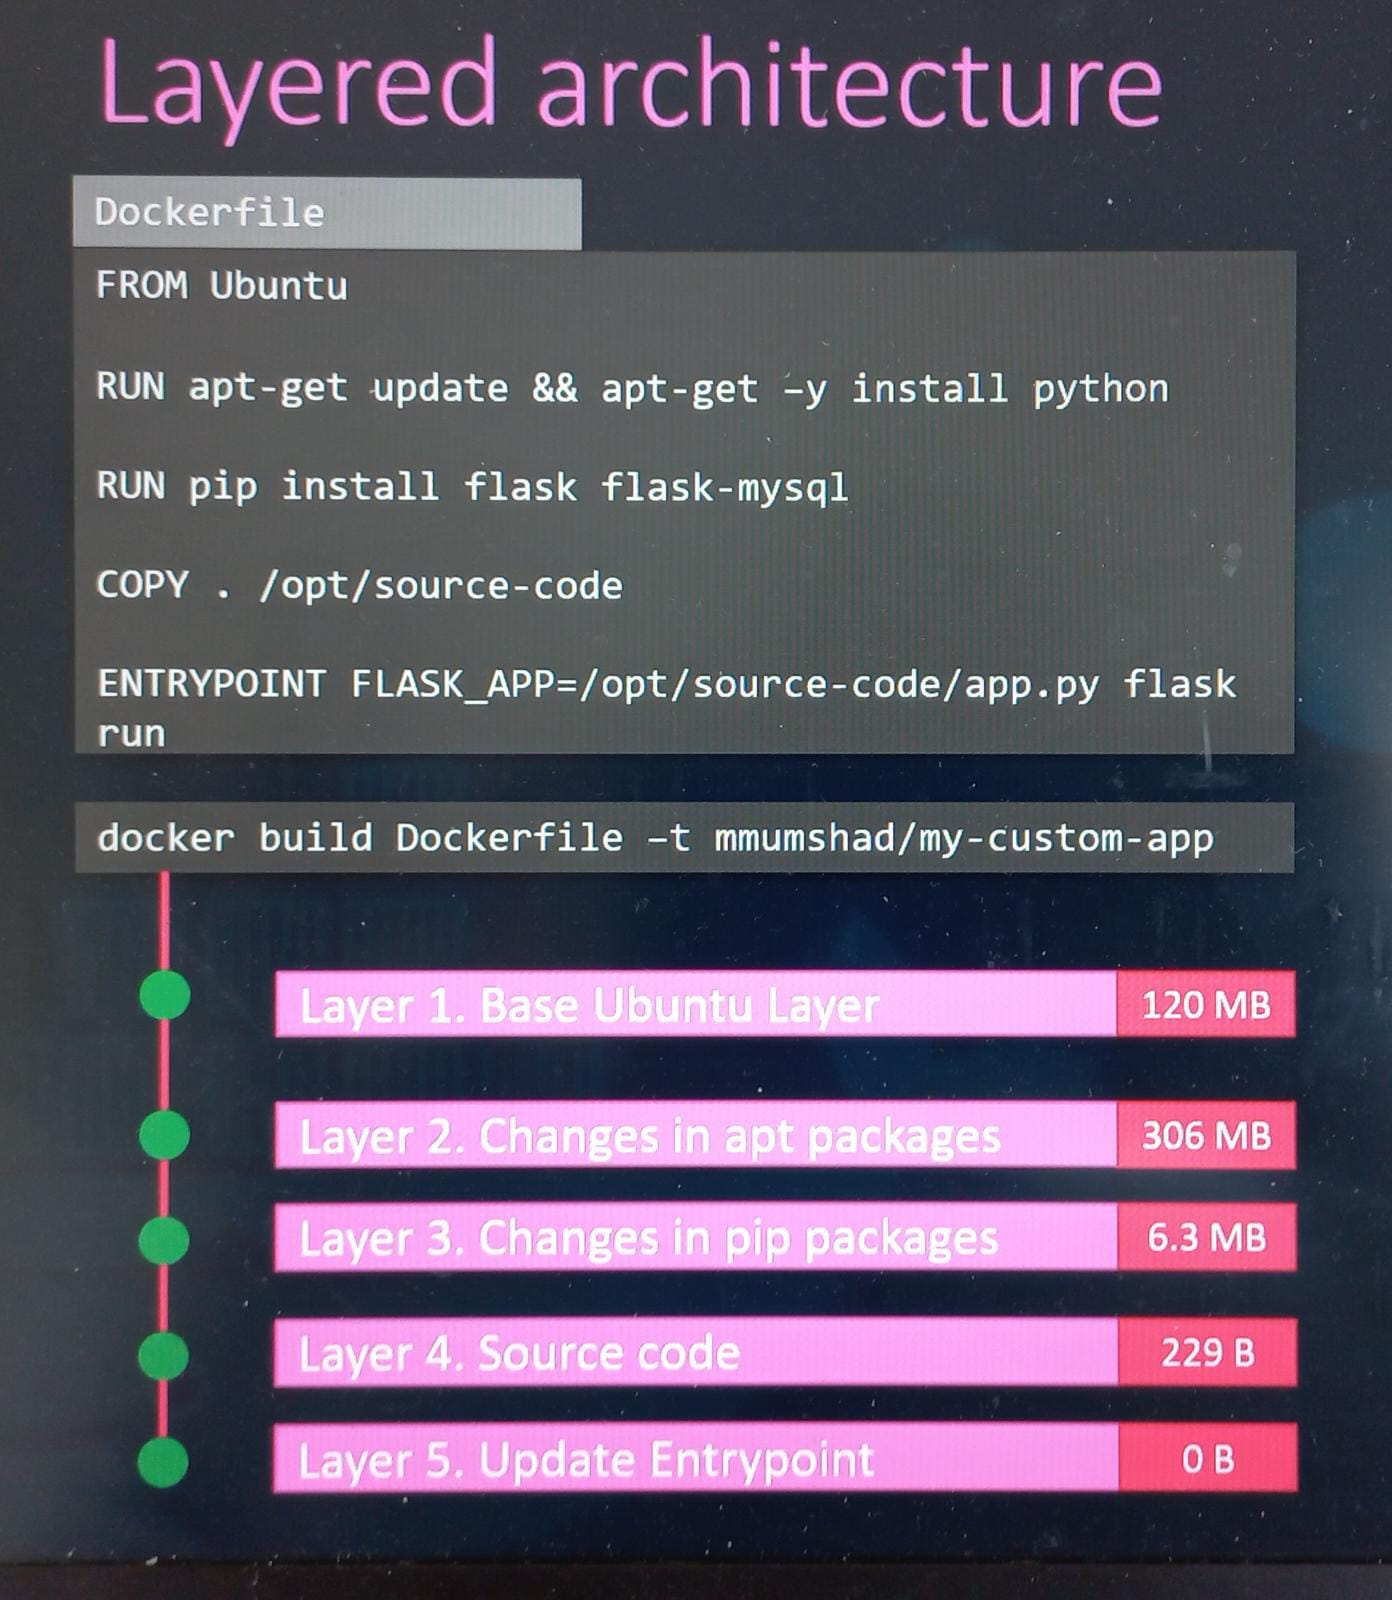
\includegraphics[scale=0.15]{pictures/st1.png}
\end{figure}

Every layer \textbf{only stores the changes from the previous layer} it is reflected in the size as well.

To understand the advantages of this layered architecture let's consider a second Dockerfile, which is different but in some parts is common. Using the same image, the same python and flask dependencies, but uses a different source code to create a different application image. When we run the \verb|docker build| command to build a new image for this application, since the first three layers of both the applications are the same, \textbf{docker is not going to build the first three layers}, instead it reuses the first 3 layers from the cache (generated with the build of the first Dockerfile). So only creates the last two layers. That is how Docker easily and efficiently saves disc space, and saves us a lot of time during builds and updates.

\begin{figure}[H]
    \centering
    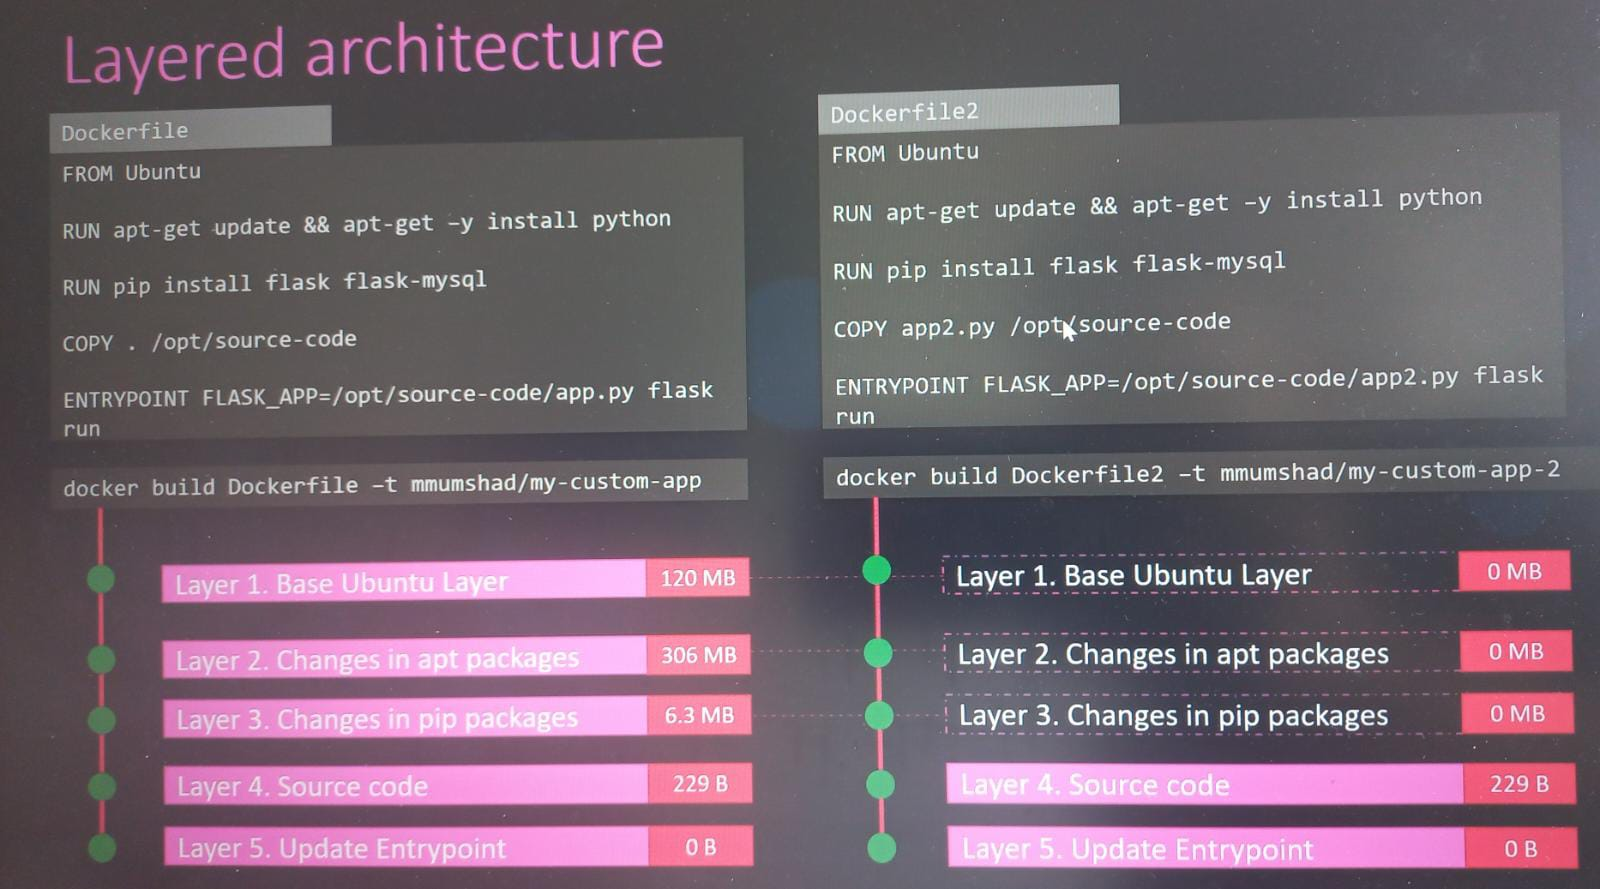
\includegraphics[width=\textwidth]{pictures/st2.png}
\end{figure}

\begin{blocktemplateII}{NOTE}
Once the image is \textbf{completely build}, we cannot modify the contents of the layers, so they are \textbf{Read Only} and we can only modify them by iniciation a new build.
\end{blocktemplateII}

When we run a container based on this images with \verb|docker run| comman, it adds a new writeable layer on the TOP of the image layer, this layer is created to store data created by the container such as:

\begin{itemize}
    \item Logs files written by the applications
    \item Any temporary files generated by the container
    \item Just any file modified by the user on that container, or by external accessing
\end{itemize}

The life of this layer though is only as long as the container is alive. So when the container is destroyed, this layer and all of the changes stored on it are also destroyed. Remember that the same image layer is shared by all containers created using this image.

So imagine that we create a container, and in the runtime environment we want to create a file called temp.txt. It will be created in the container layer, but it won't take effect over Image Layers, so if we run a container with the same image, this file will not be created. Furthermore, if we for example modify the source code application that was created inside the Image Layer, it will only be modified in the Container Layer, so if we run another container with the same image the modification will not take effect. This is because when we modify some file in the Image Layer, Docker automatically creates a copy of that file in the Container Layer (it is invisible for the user but it happens), so we can play with this file as we want but never modify the image ones.

As we said, when a containers is destroyed, all the data stored in the Container Layer is automatically removed, the change in the app code, or the files we have created, all disappears. That's why we wanted to Persist the Data.

\subsubsection{Volumes in Docker}
\label{dockmount}
Imagine we want to create a DB container, so we obviously want to preserve the data created in the Container Layer, as long as it is a DB, and users, applications and other servers will be constantly modifying its content. So it has to be resilient to restarts, and independent to the containers created. If the container restarts it must have the data it has when he died, and all the containers running the DB image must have the same data, for data consistency. For that purpose, \textbf{Docker has Persisnt Volumes}.

\paragraph{Volume Mounting}

The first step is to \textbf{mount a Docker Volume}, to tell Docker to creates a folder:

\verb|/var/lib/docker/volumes/data_volume|:

\begin{codetemplate}{}
\begin{verbatim}
$ docker volume create data_volume
\end{verbatim}
\end{codetemplate}

Then have to pass it as an argument when we run the container:
\begin{codetemplate}{}
\begin{verbatim}
$ docker run -v data_volume:/var/lib/mysql mysql1.0.0
\end{verbatim}
\end{codetemplate}

So this way, we create a Symbolic Link between docker container path and our local path, so every change made by the database container will be written in the local folder. Even if the container is destroyed the data is still here.

\begin{blocktemplate}{NOTE}
But what would happen if we use the run command without having created a Docker volume previously?
\begin{codetemplate}{}
\begin{verbatim}
$ docker run -v data_volume_2:/var/lib/mysql mysql1.0.0
\end{verbatim}
\end{codetemplate}

Docker is so intelligent and will create before running the container the Persistent Volume, and then, create the link between the local folder and the container.
\end{blocktemplate}

To see all the Persistent Volumes created by Docker:
\begin{codetemplate}{}
\begin{verbatim}
$ docker volume ls
\end{verbatim}
\end{codetemplate}

Or:
\begin{codetemplate}{}
\begin{verbatim}
$ ls -la /var/lib/docker/volumes/
\end{verbatim}
\end{codetemplate}

To inspect specific volume:
\begin{codetemplate}{}
\begin{verbatim}
$ docker volume inspect volume_name
\end{verbatim}
\end{codetemplate}

\paragraph{Bind Mounting}

But what happen if we have our data already at another location? For example in our local folder, inside the application directory, under /data and we want to share this data as a volume with the container (maybe to do some tests), and not in the default \verb|/var/lib/docker/volumes/| folder. In this case we will use the docker run command with -v without creating a Volume, but in this case we must to provide the complete or relative path to the folder we would like to mount:

\begin{codetemplate}{}
\begin{verbatim}
$ docker run -v /users/titocampis/alexwork/appmysql/data:/var/lib/mysql mysql1.0.0
\end{verbatim}
\end{codetemplate}

\begin{codetemplate}{}
\begin{verbatim}
$ docker run -v data:/var/lib/mysql mysql1.0.0
\end{verbatim}
\end{codetemplate}

\paragraph{Volume Mounting vs Bind Mounting}

\textbf{Volume Mount:} It mounts a Volume from the volumes directory.

\textbf{Binding Mount:} It mounts a Volume from any other location in the Docker Host.

\paragraph{The correct way: run --mount}

\begin{blocktemplateI}{NOTE}
In the new versions of Docker, the correct way to mount a volume (Bind or not) inside a container is using the option \verb|--mount|
\begin{codetemplate}{}
\begin{verbatim}
$ docker run \
    --mount type=bind,source=/data/mysql,target=/var/lib/mysql \ 
    mysql:1.0.0
\end{verbatim}
\end{codetemplate}
\begin{codetemplate}{}
\begin{verbatim}
$ docker run \
    --mount type=mount,source=mydata,target=/var/lib/mysql \ 
    mysql:1.0.0
\end{verbatim}
\end{codetemplate}
\end{blocktemplateI}

\subsubsection{Storage Drivers \& Volume Drivers}

\paragraph{Volume Driver Plugins}
They are in charge of manage volumes, by default it is \textbf{local}, but there are many other third party plugins which allow we to create a volume on third-party solutions, like:
\begin{itemize}
    \item Azure File Storage.
    \item Convoy.
    \item DigitalOcean Block Storage.
    \item Flocker.
    \item gce-docker.
    \item ClusterFS.
    \item Portworx.
    \item etc.
\end{itemize}

\begin{codetemplate}{}
\begin{verbatim}
$ docker run ... --volume-driver <volume_driver_name>
\end{verbatim}
\end{codetemplate}

\paragraph{Storage Drivers}
\textbf{Storage Drivers} help to manage storage on images and containers, they don't manage volumes.
\begin{itemize}
    \item Maintining the layered architecture
    \item Creating a writable layer
    \item Moving files across layers to enable copy and write 
    \item etc.
\end{itemize}

Docker uses Storage Drivers to enable layered architecture, some of the common storage drivers are: AUFS, ZFS, BTRFS, Device Mapper, Overlay, Overlay2. The decistion of which use depens on the underlying SO (Ubuntu, IOS, Windows, etc.).

\subsection{K8s CSI (Container Storage Interface)}

In the past K8s used Docker alone as the container runtime engine, and all the code to work with Docker was embedded within the K8s Cluster source code. But with other container runtimes comming ins as: Rocket and CRI-O, it was important to open up and extend support to work with different container runtimes and no be dependent on the K8s source code. And that's why \textbf{Container Runtime Interface (CRI)} came to be. It is a standard that defines how an orchestration solution like K8s would communicate with container runtimes like Docker, so in the future if a new container runtime interface is developed, they can simplify follow the CRI standards and that new container runtime would work with K8s.

It is similary to the extension of CNI (Container Networking Interface), to extend the support for different Networking Solutions. Now any Networking vendors could simply develop their plugin based on the CNI standards and make their solution work with K8s.

\begin{figure}[H]
    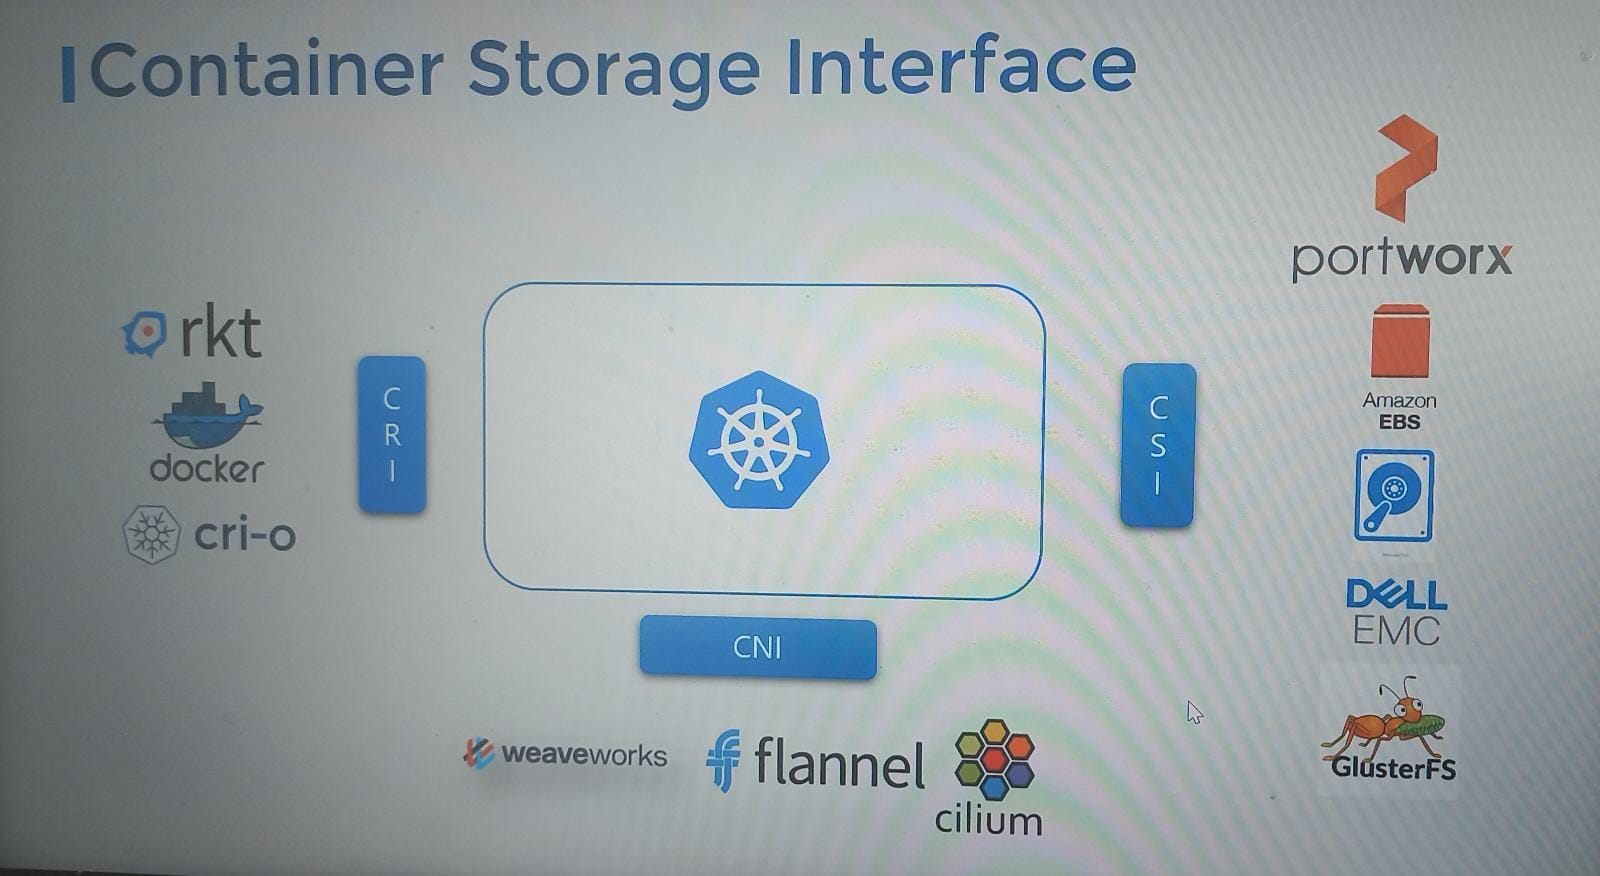
\includegraphics[width=\textwidth]{pictures/st3.png}
\end{figure}

So as we can imagine, CSI (Container Storage Interface) was developer to support multiple storage solutions, with CSI we can now write our own drivers for our own storage to work with K8s. Port Works, Amazon EBS, Azure Desk, etc. Everyone's got their own CSI drivers.

CSI is not a K8s standard, it is meant to be a Universal Standard, and if implemented will allow any orchestration tool,
to work with any storage vendor with a supported plugin.

CSI defines a set of RPC's (Remote Procedure Call), that will be created by the container orchestation tool
to be implemented by the storage drivers.
\begin{itemize}
    \item Call to provision a new volume.
    \item Call to delete a volume.
    \item Call to provision a new volume on the storage.
    \item Call to decomission volume on the storage.
    \item Call to make the available volume visible to a Node.
\end{itemize}

\subsection{K8s Volumes \& Persistent Volumes}

\subsubsection{Docker Volumes}

Docker containers are meant to be transient in nature, which means they are meant to last only for a short period of time. They are designed to process, recieve, modify and do thing with this data but destroy all data once finished, the data is destroyed along with the container. To persist data processed by the containers we attach a volume to the container when they are created, as we saw in section \ref{dockmount}. 

So the data processed by containers are now stored in this volume, retaining it permanently.

\begin{figure}[H]
    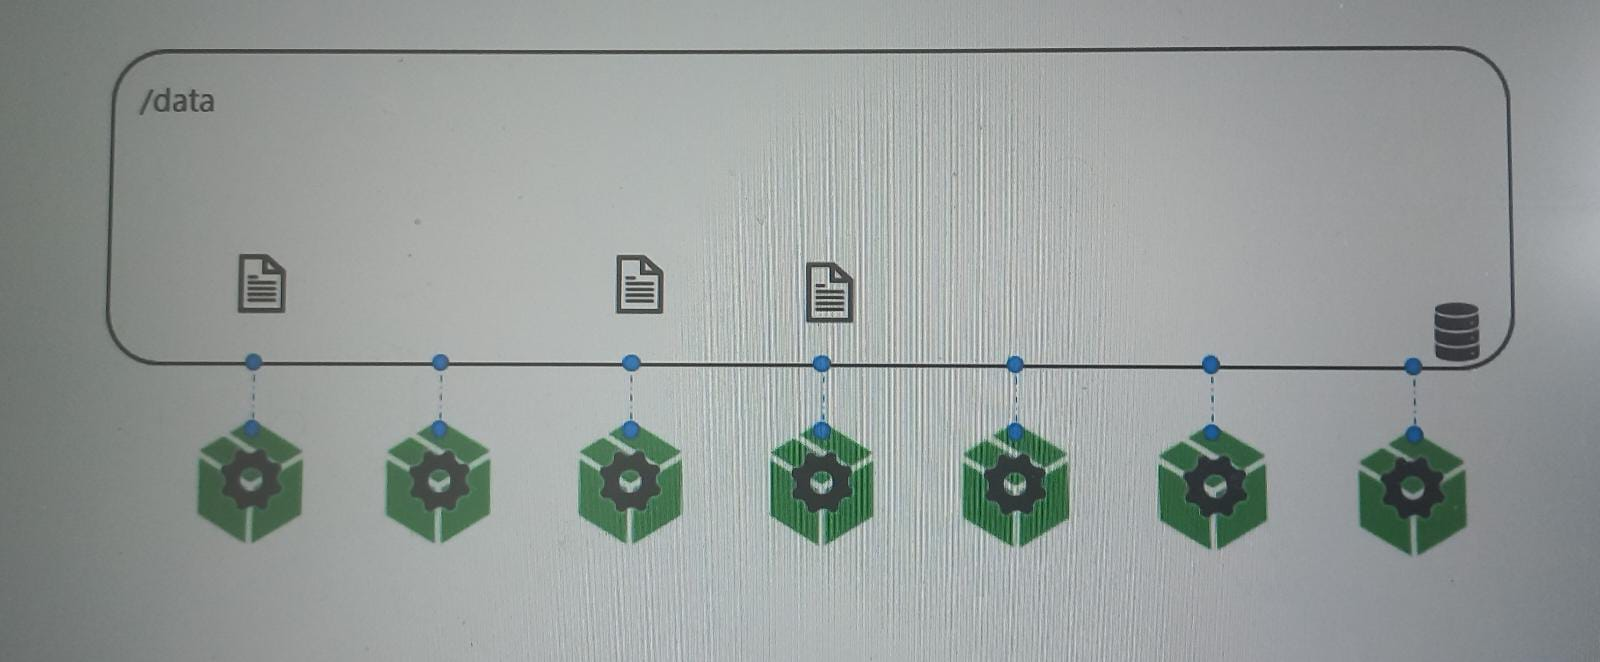
\includegraphics[width=\textwidth]{pictures/st4.png}
\end{figure}

\subsubsection{K8s Volumes}

How does it works in K8s world? Just as in Docker, the Pods created on K8s are transient in nature, when a pod is created it manages data and when it is destroyed, all its data is destroyed as well. \textbf{In order to persist data, we attach Volumes to the Pods}, so data generated by the POd is now stored in the Volume, and even after the Pod is deleted, the data remains.

\paragraph{Creating a K8s Volume}

Imagine we have a Pod that runs an image inside a container which has a command that generates a random number and stores it under \verb|/opt/number.out|. If the Pod is generated without a volume, the data will be stored inside the Pod, but when the Pod dies, the data will be removed.

\textbf{.spec.volumes}

In order to retain the number generated by the Pod, we create a \textbf{volume} inside the Pod in  \textbf{.spec.volumes}. There are multiple configurations, but for now, we are going to configure it to use a directory on the host. This way all the files stored in the directory on the Pod will be stored in the directory data on the Node where the Pod is running.

\textbf{.spec.containers.volumeMounts}

But that's not all,  we have to mount this volume inside the container in order to container can use it.

\begin{codetemplate}{}
\begin{verbatim}
apiVersion: v1
kind: Pod
metadata:
    name: random-number-generator
spec:
    containers:
    - image: alpine
      name: alpine
      command: ["/bin/bash","-c]
      args: ["shuf -i 0-100 -n 1 >> /opt/number.out;]
      ...
      volumeMounts:
      - mountPath: /opt
        name: data-volume
    volumes:
    - name: data-volume
      hostPath:
        path: /data
        type: Directory
\end{verbatim}
\end{codetemplate}

Now yes, the random number will be written in the \verb|/opt/number.out| container directory and in the Node directory \verb|/data|. When the Pod dies, the random number file still lives on the Node.

But we can imagine this is not suitable, because if the Pod restarts and now is allocated in another Node, the data will be lost!! Because it is only on the last Node. For that the solution involves 2 actors:

\textbf{Use external shared storage solutions to share storage between nodes:} K8s supports several types of different shared storage solutions as:
\begin{itemize}
    \item NFS
    \item GlusterFS
    \item Flocker
    \item Ceph
    \item AWS
    \item Google Persistent
\end{itemize}

\paragraph{Example of use external shared storage solution}

If we are using the AWS shared storage solution:
\begin{codetemplate}{}
\begin{verbatim}
...
volumes:
- name: data-volume
  awsElasticBlockStore:
    volumeID: <volume-id>
    fsType: ext4
\end{verbatim}
\end{codetemplate}

\subsubsection{K8s Persistent Volumes}

\href{https://kubernetes.io/docs/concepts/storage/persistent-volumes/}{Official K8s Doc}

It is a way of manage the storage more centrally, we would like it to be configured in a way that an administrator can create a large pool of storage and then have users carve out pieces from it as required. That is where \textbf{Persistent Volumes} can help.

A Persistent Volume is a cluster-wide pool of storage volumes configured by an administrator to be used by users deploying applications on the cluster. The users can now select storage from this pool using \textbf{Persistent Volume Claims}

\begin{figure}[H]
    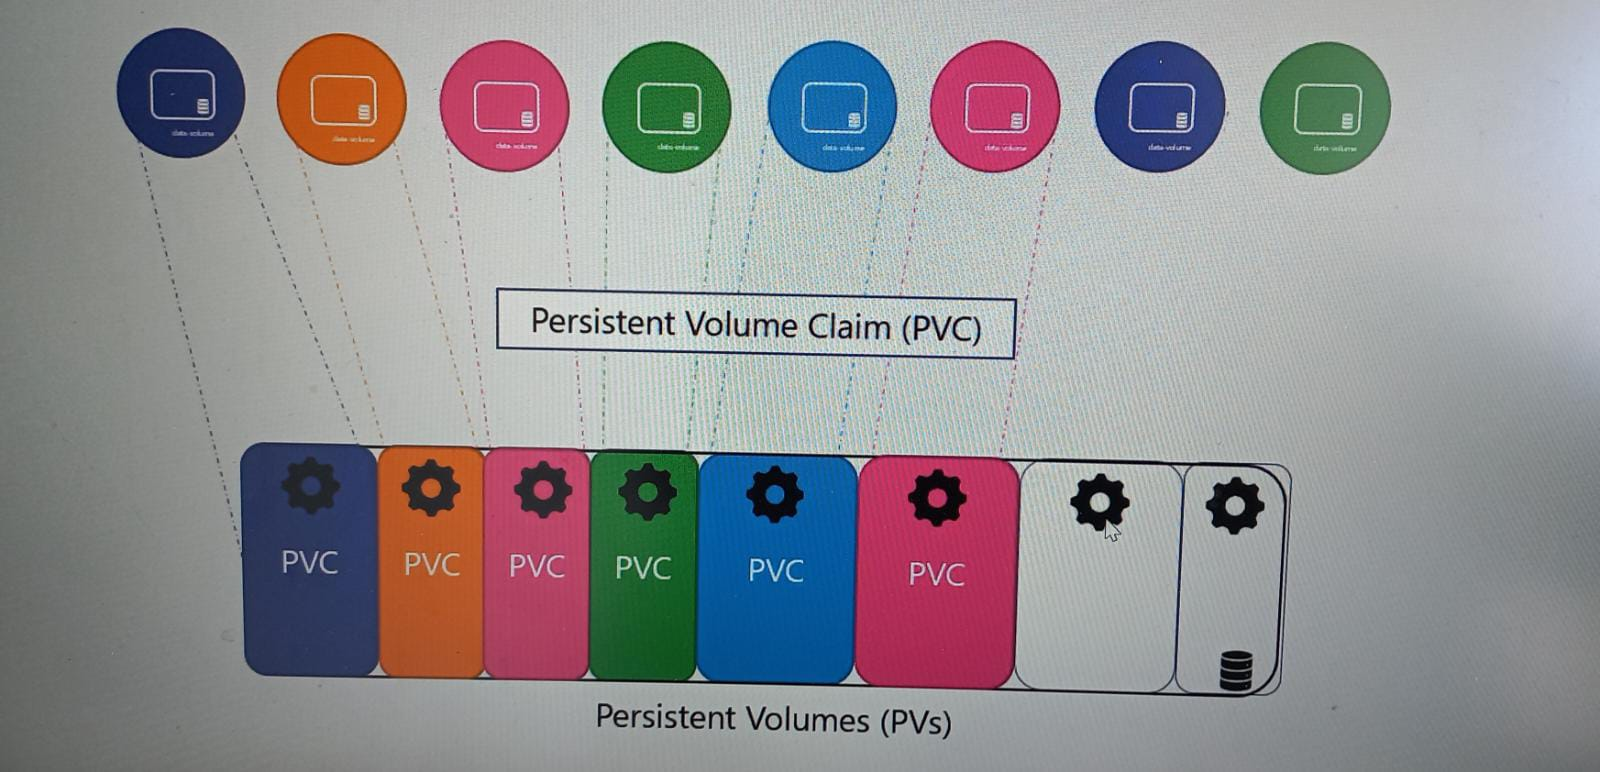
\includegraphics[width=\textwidth]{pictures/pv.png}
\end{figure}

\paragraph{Creating a Persistent Volume}

\begin{codetemplate}{pv-template.yaml}
\begin{verbatim}
apiVersion: v1
kind: PersistentVolume
metadata:
  name: pv-log
spec:
  capacity:
    storage: 100Mi
  accessModes:
  - ReadWriteOnce
  capacity:
    storage: 1Gi
  hostPath:
    path: /tmp/data
\end{verbatim}
\end{codetemplate}

\textbf{accessMode}

Defines how a volume should be mounted on the hosts, read-only, read-write, etc. The supported values are:
\begin{itemize}
    \item \textbf{ReadOnlyOnce:} the PV will be read-write by a single node, it only can be read from resources inside the same node.
    \item \textbf{ReadOnlyMany:} the PV will be read-only by resources in many nodes.
    \item \textbf{ReadWriteMany:} the PV will be the volume read-write by many nodes.
\end{itemize}

\begin{blocktemplateIII}{WARNING}
hostPath option must not be used in Production Environments, because it means we are associating the storage of the current Node where we are creating the Persistent Volume.

To avoid that, we can replace with one of the supported storage solutions as we saw in the previous section, for example:
\begin{codetemplate}{pv-template.yaml}
\begin{verbatim}
...
    capacity:
        storage: 1Gi
    awsElasticBlockStore:
        volumeID: <volume-id>
        fsType: ext4
\end{verbatim}
\end{codetemplate}

\end{blocktemplateIII}

\begin{codetemplate}{}
\begin{verbatim}
$ kubectl create -f pv-template.yaml
\end{verbatim}
\end{codetemplate}

\begin{codetemplate}{}
\begin{verbatim}
$ kubectl get pv
\end{verbatim}
\end{codetemplate}

\subsection{K8s Persistent Volume Claims}

\href{https://kubernetes.io/docs/concepts/storage/persistent-volumes/#persistentvolumeclaims}{Official K8s Doc}

As we saw in the previous section, \textbf{Persistent Volume Claims} are the K8s objects that makes \textbf{Persistent Volumes} available on the Nodes. PV's and PVC's are two separate objects in the K8s Namespace. An administrator creates a set of PV'se, and a user creates PVC's to use the storage.

\begin{blocktemplateIII}{WARNING}
PV's are not attached to any Namespace, they are across all Namespaces, but it can have permisions of view depending on the role. It is recommended to only have read-writte acces to this objects by Cluster Aminsitrators.
\end{blocktemplateIII}

Once the PVC's are created, K8s binds (vincula) the PV's to claims based on the request and properties set on the volume. Every PVC must be bounded to a single PV, during the binding process, K8s tries to find a PV that matches the following requests of the PVC's:

\begin{itemize}
    \item has sufficient capacity
    \item has same access modes
    \item has same volume modes
    \item has same Storage Class
\end{itemize}

However, if there multiple possible matches for a single claim, and we would like to specifically use a particular PV, we could still use \textbf{labels and selectors} to bind to the right PV's.

\begin{blocktemplateIII}{WARNING}
Remember the relationship between PV's and PVC's is one to one, so there cannot be more than one PVC binded to a PV. If the PVC requires less storage than the PV storage, no other PVC's can uses the remaining capacity in the volume. If there are not available Volumes that matches the PVC, it will remain in a Pending State until newe volumes are made available on the Cluster, and when that happens, the PVC is automatically bounded.
\end{blocktemplateIII}

\subsubsection{Creating a Persistent Volume Claim}

\begin{codetemplate}{pvc-template.yaml}
\begin{verbatim}
apiVersion: v1
kind: PersistentVolumeClaim
metadata:
  name: myclaim
spec:
  accessModes:
  - ReadWriteOnce
  resources:
    requests:
      storage: 500Mi
\end{verbatim}
\end{codetemplate}

\begin{codetemplate}{}
\begin{verbatim}
$ kubectl get pvc
\end{verbatim}
\end{codetemplate}

\begin{blocktemplate}{NOTE}
If we pay attention on what we see when get pvc, we can see the PV attached to that pvc.
\end{blocktemplate}

\begin{blocktemplateIII}{WARNING}
If the \textbf{accessModes} do not match, the \textbf{PVC} will not be binded to the \textbf{PV}.
\end{blocktemplateIII}

\subsubsection{Deleting Persistent Volume Claims}

Just use the  \verb|kubectl delet pvc <name>| command. But what happens with the underlying PV? we can choose what is to happen to the PV. By defaul it is set to retain, meaning the PV will remain until it is manually deleted by the administrator and it is not available for reuse by any other claims anymore, it is so romantic.

Also, we can change the default configuration:

\begin{codetemplate}{pv-template.yaml}
\begin{verbatim}
apiVersion: v1
kind: PersistentVolume
metadata:
    name: pv-vol1
spec:
    accessModes:
    - ReadWriteOnce
    capacity:
        storage: 1Gi
    hostPath:
        path: /tmp/data
    persistentVolumeReclaimPolicy: Recycle
    # Default persistentVolumeReclaimPolicy: Retain
    # persistentVolumeReclaimPolicy: Delete
\end{verbatim}
\end{codetemplate}

If we use \textbf{Delete} option the PV will be deleted as soon as the PVC is deleted, freeing up storage on the end storage device. If we use \textbf{Recycle} the data in the data volume will be scrubbed before making it available to other claims.

\paragraph{Associating PVC's to Pods to containers can cosume them}

Once we create a PVC use it in a POD definition file by specifying the PVC Claim name under persistentVolumeClaim section in the volumes section like this:

\begin{codetemplate}{}
\begin{verbatim}
apiVersion: v1
kind: Pod
metadata:
    name: random-number-generator
spec:
    containers:
    - image: alpine
      name: alpine
      command: ["/bin/bash","-c]
      args: ["shuf -i 0-100 -n 1 >> /opt/number.out;]
      ...
      volumeMounts:
      - mountPath: /opt
        name: data-volume
    volumes:
    - name: data-volume
      persistentVolumeClaim:
        claimName: myclaim
\end{verbatim}
\end{codetemplate}

\begin{blocktemplateIII}{WARNING}
It is not necessary to create a PV object to share storage bare between a Pod and the Node. It's enough to create volume in the specs of the Pod an a volumeMount in the container, and we will do the same it does docker, in our system. 

But this only applies to bare shared storage between a Node an a Pod, if we want to persist the storage between all Nodes it is more complex, so we have to create PV's and PVC's.
\end{blocktemplateIII}

\begin{blocktemplateIII}{WARNING}
If there is storage let over in the PV, the PVC will get in all.
\end{blocktemplateIII}

\begin{blocktemplateIII}{WARNING}
The PVC must be in the same Namespace as the Pod, if it is not like that, it won't work.
\end{blocktemplateIII}

\begin{blocktemplateIII}{WARNING}
If we try to delete a PVC used by a Pod, it won't be definitely deleted until the Pod dies. In will remain in Terminating state.
\end{blocktemplateIII}

\textbf{What happens if we modify, remove, or add files to the shared directory?}

Wow, if we add files in the local directory they are added automatically to the pod:

Y lo mismo sucede al reves!!! WOOOOOW!!! Quedan automagicamente conectados para siempre. Amigos para siempre do we want to be my friend...

\subsection{Storage Class}

In the previous sections, we discussed about how to create PV's an then create PVC's to claim that storage, and then use the PVC's in the Pod definition files as volumes. The problem here is before the PV's are created disk storage must be created on the Cloud Platform (Google, Azure, IBM, AWS, etc.). So every time an application requires storage it is needed to manually provision the disk and after create manually a PV using the definition file using the same name as the disk we have already created. This is called static provisioning volumes.

It will be amazing if the volume is provisioned automatically when the application requires it, and that is where \textbf{StorageClass} come in. With \textbf{StorageClass} we can define a provisioner like google storage which automatically provision storage on the cloud and attach that to Pods when the claim is made. It is called dynamic provisioning on Pods. we do that by creating an Object \textbf{StorageClass}.

\begin{codetemplate}{sc-template.yaml}
\begin{verbatim}
apiVersion: storage.k8s.io/v1
kind: StorageClass
metadata:
    name: object-storage
provisioner: kubernetes.io/gce.pd
\end{verbatim}
\end{codetemplate}

We use the provisioner \verb|kubernetes.io/gce.pd| to create a Volume on GCP. There are other any provisioners as well, as AWS EBS, Azure File, Azure Disk, Portworx, etc. With each of these provisioners, we can pass in additional parameters such as the type of disk to provision, the replication type, etc. These parameters are very specific to the provisioner that we are using.

If we use \textbf{StorageClass} we no longer need the PV definition, because the PV and any associated storage is going to be associated automatically when the StorageClasses created. But we have to let the PVC know about the StorageClass, so:

\begin{codetemplate}{}
\begin{verbatim}
apiVersion: v1
kind: PersistentVolumeClaim
metadata:
    name: claim-log-1
spec:
    accessModes:
    - ReadWriteOnce
    storageClassName: <name-of-storage-class>
    resources:
        requests:
            storage: 50Mi
\end{verbatim}
\end{codetemplate}

With this definition, the \textbf{StorageClass} associated to the PVC uses the defined provisioner to provision a new disk with the required size.

\begin{blocktemplateIII}{WARNING}
The \verb|storageClassName| works similarly to accessMode, if the PVC has one defined, it cannot be bound to a PV that has another one defined or which does not have any defined. PV and PVC accessMode must match. 
\\\\
If the PVC has no accessMode it cannot be assignet to a PV defined with an accessMode.
\end{blocktemplateIII}

\begin{blocktemplateIII}{WARNING}
If the Storage Class makes use of VolumeBindingMode set to WaitForFirstConsumer, it will delay the binding and provisioning of a PersistentVolume until a Pod using the PersistentVolumeClaim is created.
\end{blocktemplateIII}

\subsubsection{Different Storage Classes}
One thing that is common is to use different \textbf{StorageClasses} deppending on the package that the enterprise or applications purchase. For example:

\begin{figure}[H]
    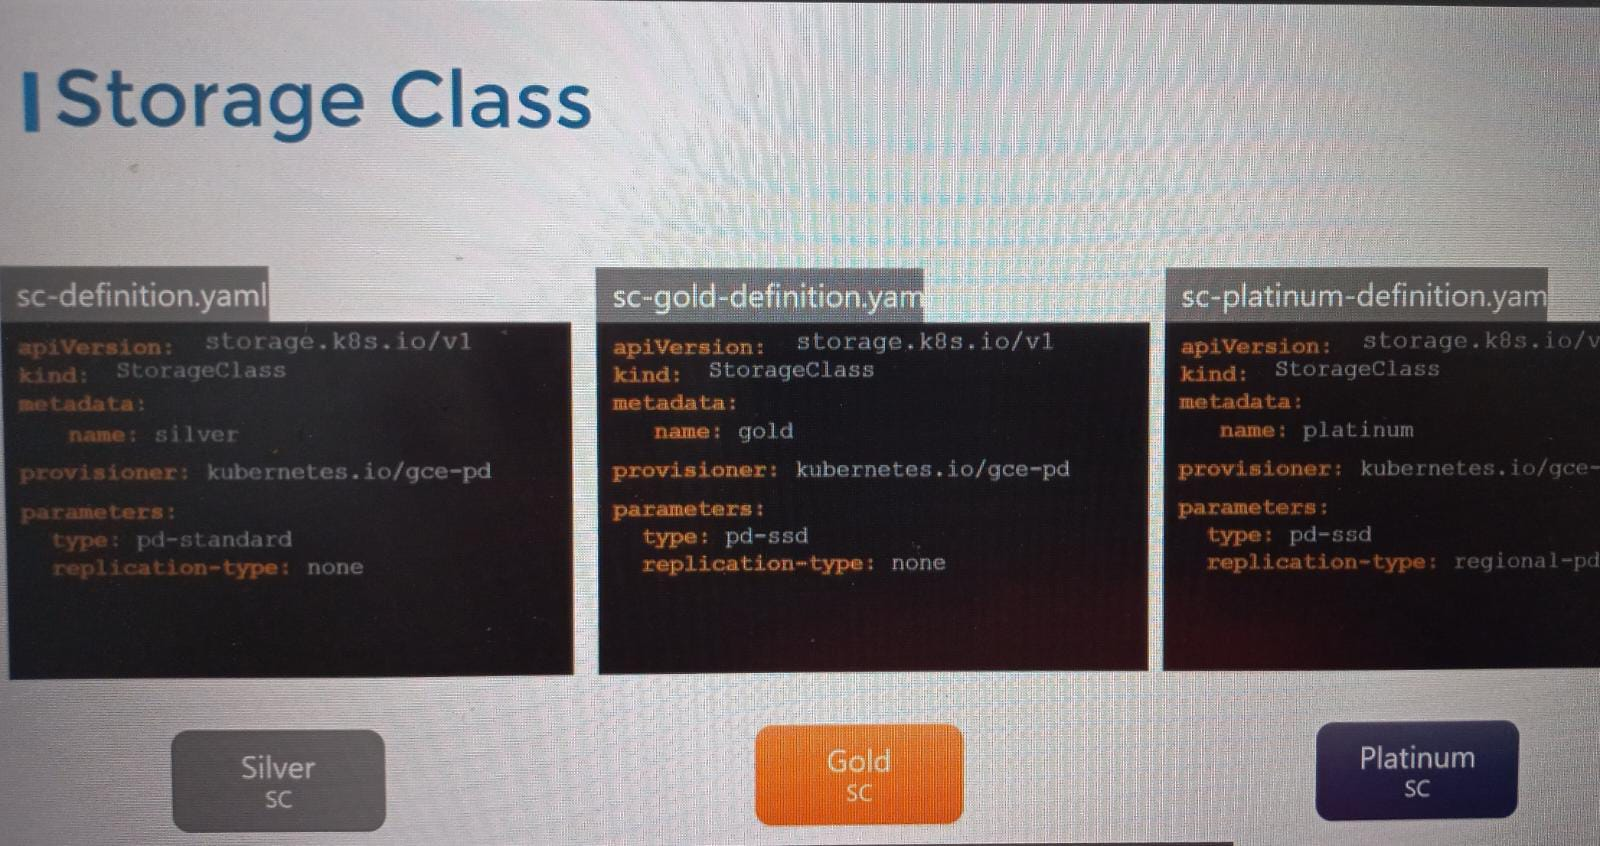
\includegraphics[width=\textwidth]{pictures/stcl.png}
\end{figure}

%======================================================
\newpage
\section{Networking Basis in Linux (not K8s)}

\subsection{Switching and routing in Linux}
\label{swrt}

\subsubsection{Switching}

What is a network? We have 2 Linux Machines, A and B, it can be: laptops, desktops, VMs on the Cloud, wherever. How does system A reach system B? So we connect them to a \textbf{switch} and it creates a network containing the two systems. 

\begin{figure}[H]
    
\includegraphics[width=\textwidth]{pictures/ntw.jpg}
\end{figure}

To connect the 2 Linux machines to a switch, we need an interface on each host (physical or virtual depending on the Host). And to see the interfaces from the Host, we use the following command:

\begin{itemize}
    \item View and managing link-layer (MAC-level) settings.
\begin{codetemplate}{}
\begin{verbatim}
$ ip link
\end{verbatim}
\end{codetemplate}

    \item Check network-layer (IP-level) details along with link-layer information.
\begin{codetemplate}{}
\begin{verbatim}
$ ip a
\end{verbatim}
\end{codetemplate}
\end{itemize}

We only want the information of \textbf{eth0} interface, which it will be used to connect the machine to the switch. 

Let's assume it's a Network with the adress 192.168.1.0, so we then assign the system with IP addresses on the same Network:

\begin{figure}[H]
    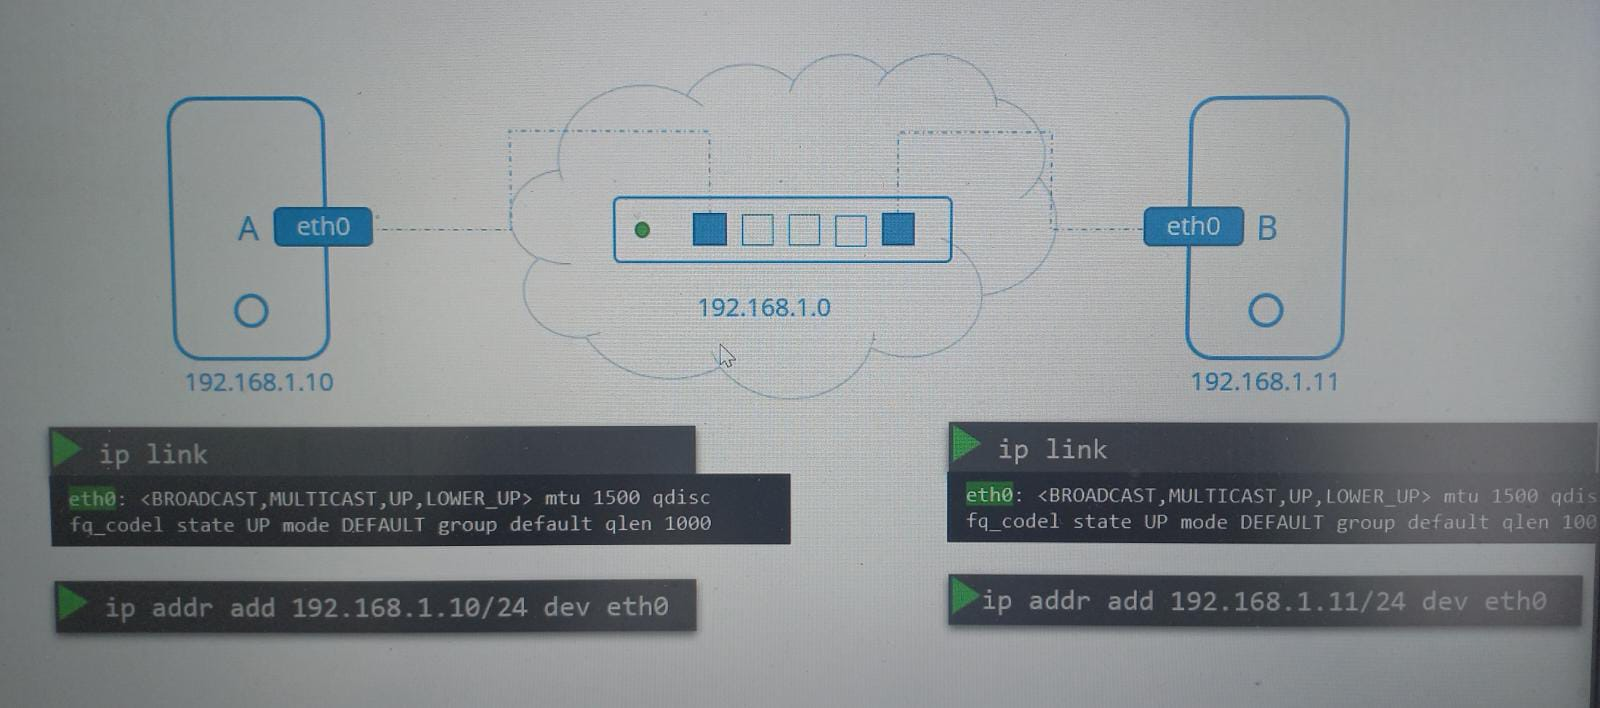
\includegraphics[width=\textwidth]{pictures/ntw2.png}
\end{figure}

To add an IP address (192.168.1.10/24) to the network interface eth0
\begin{codetemplate}{}
\begin{verbatim}
$ ip addr add 192.168.1.10/24 dev eth0
\end{verbatim}
\end{codetemplate}

Once the links are up and the IP addresses are assigned, the computers can now communicate with each other through the switch. The switch can only enable communication within a Network, which means it can receive packets from a Host on the Network and deliver it to other systems within the same Network.

\subsubsection{Routing}

Imagine we have another 2 machines in another Network at adress 192.168.2.0 and system adress according to this adress. How does a system in one Network reach a system in another Network?

Using \textbf{Routers}, a \textbf{Router} is an intelligent device which can connect two networks together. Is like another server with a lot of \textbf{Network Ports}. Since it connects to the two separate Networks it gets 2 IPs assigned, one on each Network, for example:

\begin{itemize}
    \item For the first Network, it receives the IP: 192.168.1.1
    \item For the second Network, it receives the IP: 192.168.2.1
\end{itemize}

\begin{figure}[H]
    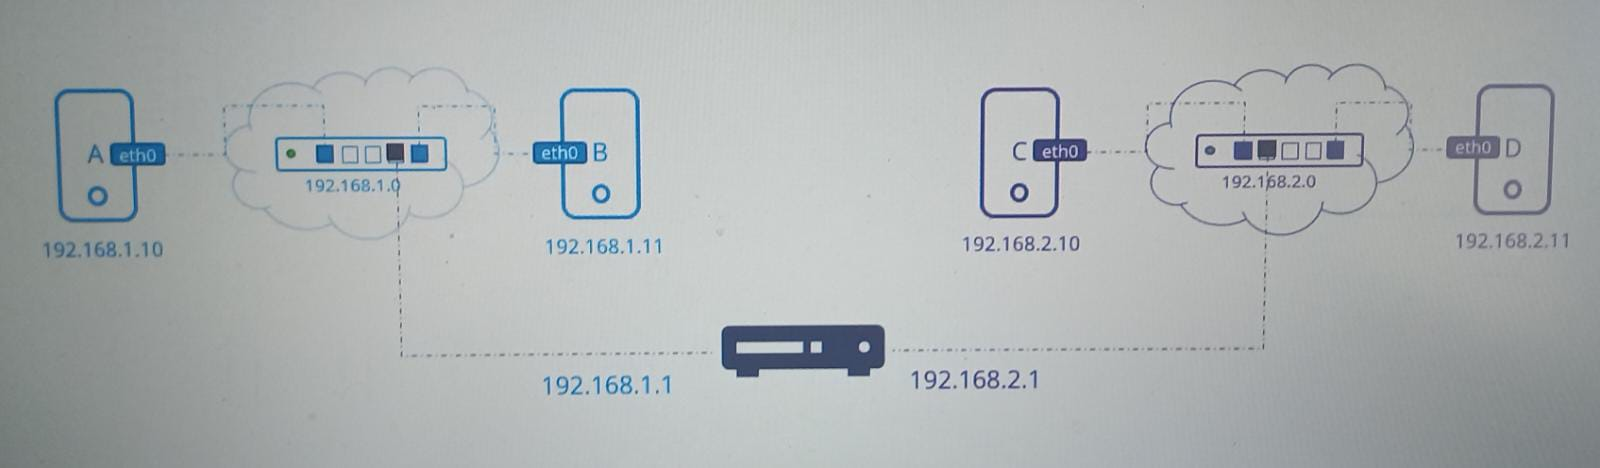
\includegraphics[width=\textwidth]{pictures/ntw4.png}
\end{figure}

Imagine that system A wants to communicate with system C. How does the system 
A know where the Router is configured on the Network to send the packages through? 
The router is just another device set on the Network with an associated IP. This is why we configure the systems with a \textbf{gateway} (\textbf{route}). If the Network was a room, the \textbf{gateway} would be the door to the external world (other Networks). The systems need to know where that door is. 

\textbf{See existing routing configuration on a system:} it displays the kenel's routing table
\begin{codetemplate}{}
\begin{verbatim}
$ route
\end{verbatim}
\end{codetemplate}

If nothing is configured, system A cannot go outside its Network, so it cannot communicate with system C or D, only with D.

\textbf{To configure a gateway in system A:}
\begin{codetemplate}{}
\begin{verbatim}
$ ip route add 192.168.2.0/24 via 192.168.1.1
\end{verbatim}
\end{codetemplate}

Specifing that to reach 192.168.2.0/24 Network, it should pass through 192.168.1.1 (the router).

As we can imagine, we have to do the same for system B, to reach system C and system D. And the same for systems C and D to reach systems A and B. Configuring a route on the Network and configure routes on the systems.

Now supose these systems need access to the internet, for example to google at 172.217.194.0. we only need to connect the router to the internet and add a new route to the systems, to pass through router to go to Google (172.217.194.0). But there are so many different sites on different Networks on the internet, so instead of adding a routing table entry for the same router's IP adress, for each of those Networks, \textbf{we can simply say for any Network that we do not know where to route, use this router as the default gateway}. And that's the key.

\begin{codetemplate}{}
\begin{verbatim}
$ ip route add default via 192.168.2.1
\end{verbatim}
\end{codetemplate}

\begin{blocktemplate}{NOTE}
Instead of the word "default" we can use 0.0.0.0, which means any IP destination.
\end{blocktemplate}

This way, any request to an IP outside of our existing Network (not defined in route table) goes to this particular router. 

\subsubsection{Private and Public Networks configuration}

So in a simple model like this, all we need is a single routing table entry with the default gateway set to the router's IP address. But if we want to manage connections with another private Network at the same time than Public Network (as internet), it gets complicated. We should have 2 routers with 2 route rules in the configured system tables, to use different routers to send the traffic depending on the Network systems want to reach.

\begin{figure}[H]
    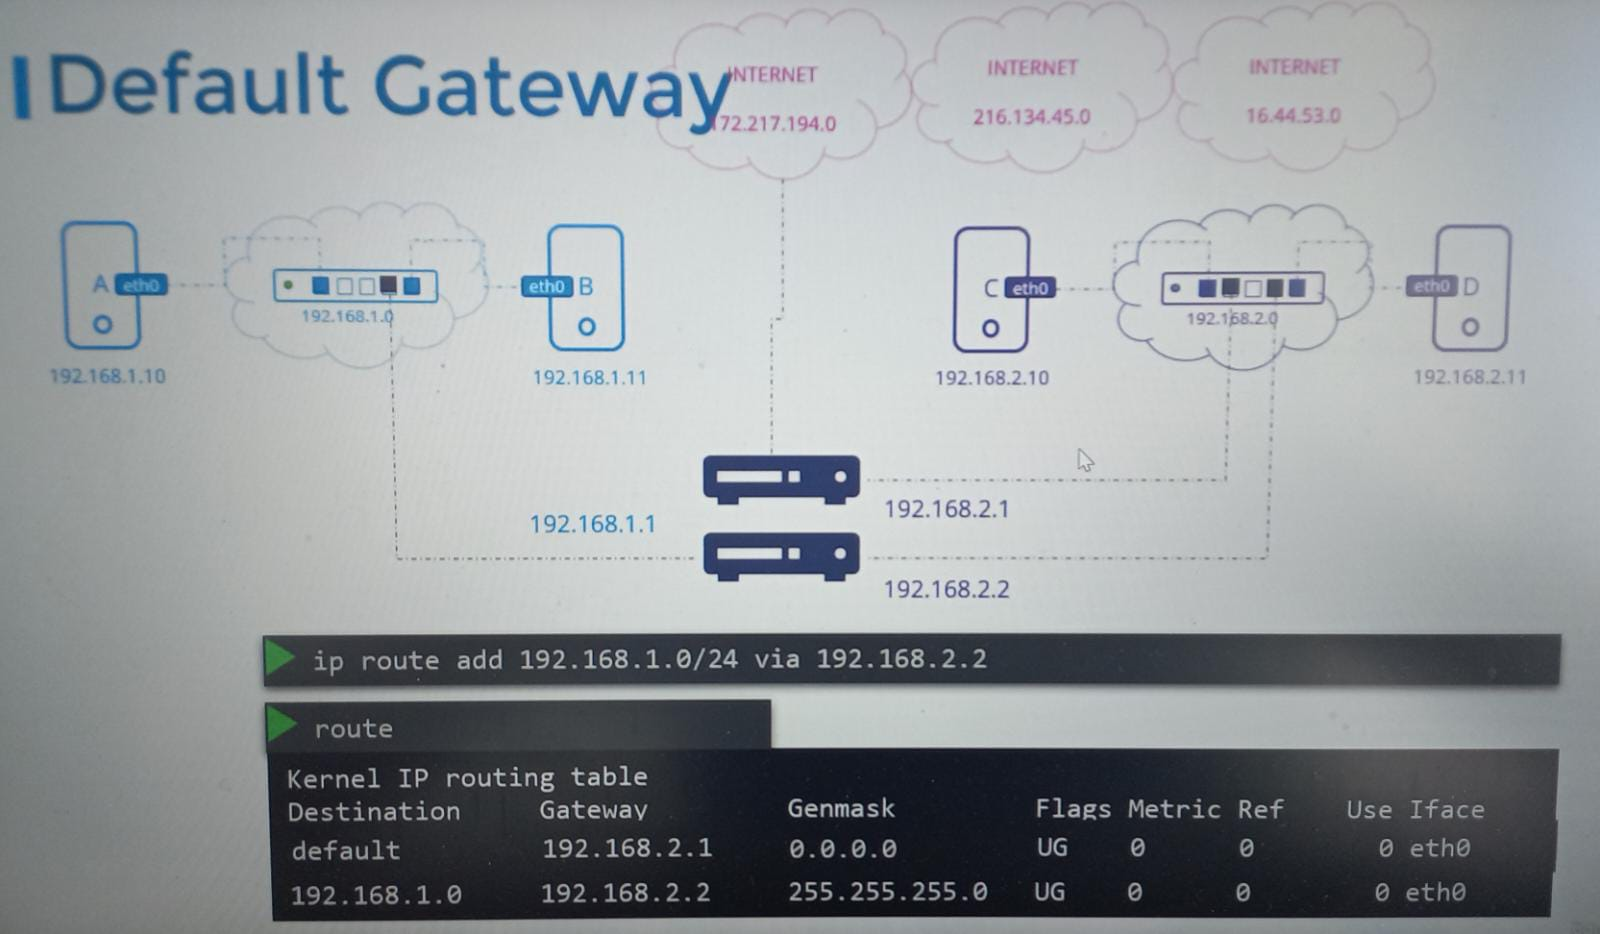
\includegraphics[width=\textwidth]{pictures/ntw5.png}
\end{figure}

\begin{itemize}
    \item One rule to connect to internal private Network on router 1
\begin{codetemplate}{}
\begin{verbatim}
$ ip route add 192.168.1.0/24 via 192.168.2.2
\end{verbatim}
\end{codetemplate}

    \item Another rule to connect to all other Networks (including internet)
\begin{codetemplate}{}
\begin{verbatim}
$ ip route add default via 192.168.2.1
\end{verbatim}
\end{codetemplate}
\end{itemize}

\subsubsection{Using a Linux System as a router}

\begin{figure}[H]
    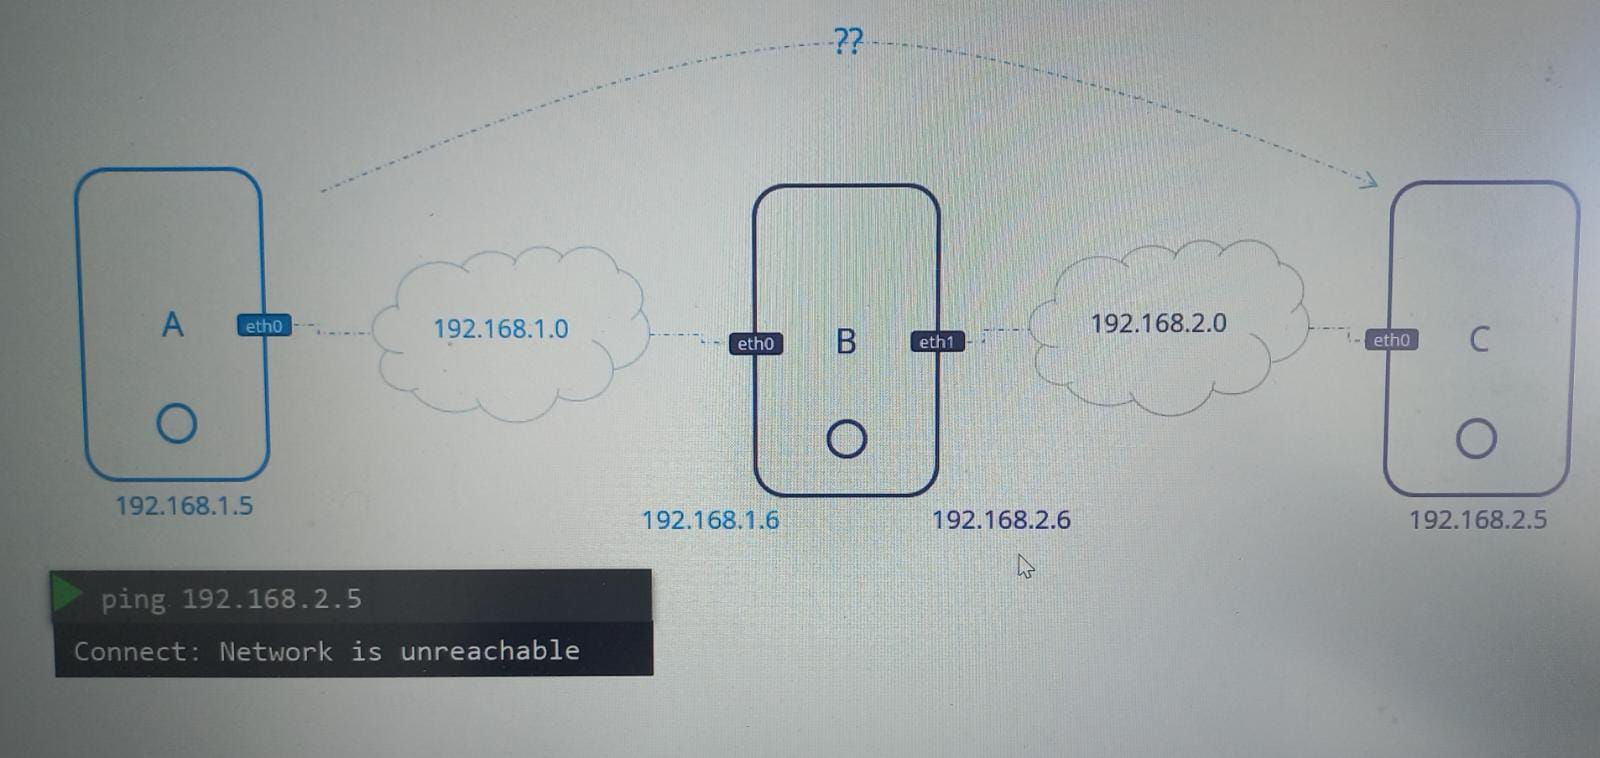
\includegraphics[width=\textwidth]{pictures/ntw6.png}
\end{figure}

As we know, Host A has no idea of how to reach Host C, because it is into another Network. So we have to say Node A to reach Host C through Node B. So we do that adding a routing rule in the table of Host A:

\begin{codetemplate}{}
\begin{verbatim}
$ ip route add 192.168.2.0/24 via 192.168.1.6
\end{verbatim}
\end{codetemplate}

When the Host C wants to response Host A will have the same issue, so we have to do the same on Host C:
\begin{codetemplate}{}
\begin{verbatim}
$ ip route add 192.168.1.0/24 via 192.168.2.6
\end{verbatim}
\end{codetemplate}

If we try to ping now, we no longer get the Network unreachable error message, that means our routing entries are right, but we still do not get any response back. This is because by deafult, in linux, packets are not forwarded from one interface to the next. For example: packets received on Eth0 of Node B are not forwarded to elsewhere thorught Eth1, for obviously security reasons. But in this case, that we know they are both secure Networks, and we want to use Node B as router, we can allow Host B to forward packets  from one Network to the other. It is set in a file on the system config:

\begin{codetemplate}{}
\begin{verbatim}
$ cat /proc/sys/net/ipv4/ip_forward
\end{verbatim}
\end{codetemplate}

\begin{itemize}
    \item \textbf{0:} No forward
    \item \textbf{1:} Forward
\end{itemize}


\begin{codetemplate}{}
\begin{verbatim}
$ echo 1 > /proc/sys/net/ipv4/ip_forward
\end{verbatim}
\end{codetemplate}

\begin{blocktemplateIII}{WARNING}
This way of configuration is not resilient to reboot, so if the system is reboot the configuration will be lost. To persist the configuration we should configure that in /etc/sysctl.conf adding:
\begin{codetemplate}{}
\begin{verbatim}
$ sudo vim /etc/sysctl.conf
###############################
...
net.ipv4.ip_forward=1
...
\end{verbatim}
\end{codetemplate}

\end{blocktemplateIII}

\subsection{DNS in Linux}

\subsubsection{Introduction to DNS}

We have 2 Hosts in the same Network, Host A and Host B. And they have been assigned a Network with IP: 192.168.1.0. So they are 192.168.1.10 and 192.168.1.11. So as we saw in the last section \ref{swrt}. As they are in the same Network, they can reach each other using their IP's. But it can be so tediously for Hosts to know all the IP's, so instead of having to remember the IP address of system B, Host A can give it a name, for example db, that when we \verb|ping db| it works like if it was using IP.

Basically we want to tell Host A that system B at IP address at 192.165.1.11 has a name db. So when db name is used, for Host A must be the same as 192.165.1.11. It can be done by adding an entry in the file \verb|/etc/hosts|:

\begin{codetemplate}{}
\begin{verbatim}
$ echo "192.168.1.11      db" >> /etc/hosts
\end{verbatim}
\end{codetemplate}

Or vim and add at the end of the file the relationship.
\begin{codetemplate}{}
\begin{verbatim}
$ sudo vim /etc/hosts
\end{verbatim}
\end{codetemplate}

So now Host A translates db as 192.165.1.11, this is called \textbf{name resolution}, associate a hostname to an IP. Whatever we put in the \verb|/etc/hosts| is the source of true for the Host. But that my not be the truth, maybe Host B is called host-2, but Host A does not care, it will follow what is in the \verb|/etc/hosts| file. 

You can make a test, associate \verb|www.google.com| hostname to IP of Host B an tst to ping, the ping will be answered by Host B. we can have any names as we want for any servers as we want in the \verb|/etc/hosts| file. Commands look into this file:

\begin{itemize}
    \item ping
    \item ssh
    \item curl
    \item nc
    \item nmap
    \item mtr
    \item ...
\end{itemize}

\subsubsection{DNS server}

In a system with few systems, we can get away with the entries of \verb|/etc/hosts| file, and this is how it was done in the past. However, when the environment grows and these files got filled with many entries we can imagine this is unmanageable. If one of the Hosts changes its IP, we are done, gj wp. This is the reason why it was decided to \textbf{move all this configuration into a single server}, who will manage all this centrally, called the \textbf{DNS server}. And then we point all hosts to look up that server if they need to resolve a hostname to an IP address instead of its own \verb|/etc/hosts| files.

How do we do that? How de we point our host to a DNS server? Imagine our DNS server has the IP 192.168.1.100, every host has a DNS resolution configuration file at \verb|/etc/resolv.conf|. So we have to add an entry into it specifying the address of the DNS server.

\begin{codetemplate}{}
\begin{verbatim}
$ echo "nameserver         192.168.1.100" >> /etc/resolv.conf
\end{verbatim}
\end{codetemplate}

Or vim and add it at the end of the file.
\begin{codetemplate}{}
\begin{verbatim}
$ sudo vim /etc/resolv.conf
\end{verbatim}
\end{codetemplate}

Once this is configured into a Host, everytime it comes up across a hostname that it does not know about, it looks it up from the DNS server. With this configuration, if the IP of any of the host was to change, we only need to change it in one file in one Host.

\begin{blocktemplateIII}{WARNING}
You can still have entries in our \verb|/etc/hosts| file, but it is not hardly recommended because it will override the configuration in \verb|/etc/resolv.conf| nameserver. Only use it when we are sure of what we are doing.
\\\\
But this is default configuration, this order can be changed in the file \verb|/etc/nsswitch.conf|
\begin{codetemplate}{}
\begin{verbatim}
$ cat /etc/nsswitch.conf
\end{verbatim}
\end{codetemplate}

\textbf{OUTPUT:} hosts:    files dns

To change this, we should modify the content on the field to invert it.
\end{blocktemplateIII}

What happens if the hostname is not found in \verb|/etc/hosts| neither in \verb|/etc/resolv.conf|, so it will fail. Unless we configure in the file \verb|/etc/hosts| of the \textbf{DNS server} to forward all unknown hostnames to the public name server on the internet (ex: 8.8.8.8).

\begin{codetemplate}{}
\begin{verbatim}
$ echo "Forward All to 8.8.8.8" >> /etc/hosts
\end{verbatim}
\end{codetemplate}

\subsubsection{FQDN}

So far, we are naming with names like db, host-1, host-2... But the real services are called: www.google.com, www.github.com, etc. They are using \textbf{FQDN's}.

\textbf{FQDN} (Fully Qualified Domain Name) or \textbf{Domain Name}, which are a complete and unique direction needed to have presence on the internet. It is composed by the name of the host and the domain, and it is used to request to specific hosts on the internet using the name resolution instead of their IP.

Let's see a FQDN structure in detail:

\begin{figure}[H]
    \centering
    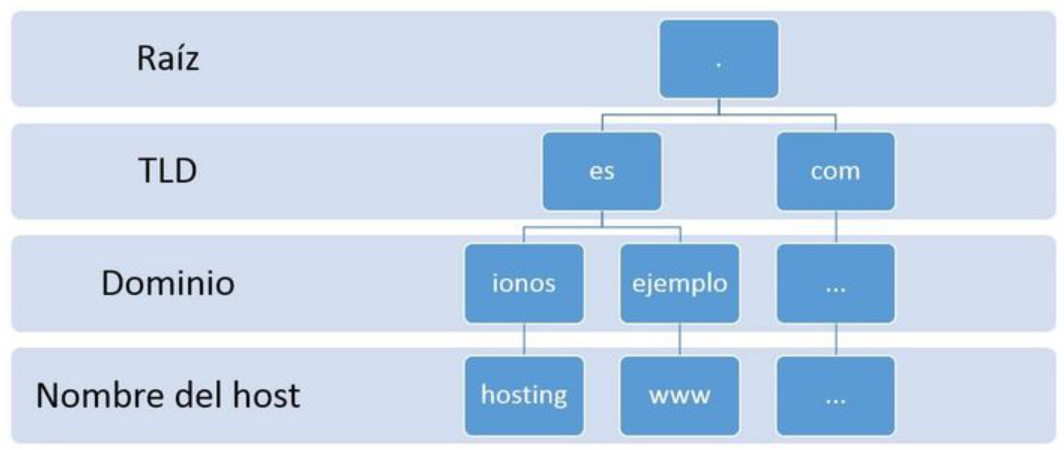
\includegraphics[scale=0.4]{pictures/image11.PNG}
\end{figure}

\begin{enumerate}
    \item \textbf{TLD (Top Level Domains):} they represent the intent or the geographical situation of the website:
    \begin{itemize}
        \item \textbf{.com:} for commercial or general purpose
        \item \textbf{.net:} for network
        \item \textbf{.edu:} for educational organizations
        \item \textbf{.es / .cat / .fr:} for geographical situation
        \item \textbf{.org:} for non-profit organizations
    \end{itemize}

    \item \textbf{Domain:} it is the hostname assigned to Google
    \item \textbf{Name of the host:} is a subdomain, which helps in further grouping things together under the Domain, for example:
    \begin{itemize}
        \item \textbf{maps.google.com:} the maps of google
        \item \textbf{drive.google.com:} the drive of google
        \item \textbf{www.google.com:} google search
        \item \textbf{mail.google.com:} google email
    \end{itemize}
\end{enumerate}

But how does this magical works in all Hosts in the world, for exampe the PC we are using. This is because when our system tries to reach any of these \textbf{FQDN's} our system first check at our \verb|/etc/hosts| or \textbf{internal DNS server}, and it normally does not know who apps or google is, so it forwards our request to
\textbf{your internet provider DNS server (you can change this on our machine configuration)}. Then the DNS Server looks at our request and forwards it to the correct host.

\textbf{Orange DNS (France)}
\begin{itemize}
    \item Primary DNS: \texttt{8.8.8.8}
    \item Secondary DNS: \texttt{8.8.4.4}
\end{itemize}

\textbf{Google Public DNS}
\begin{itemize}
    \item Primary DNS: \texttt{8.8.8.8}
    \item Secondary DNS: \texttt{8.8.4.4}
\end{itemize}
    
\textbf{Cloudflare DNS}
\begin{itemize}
    \item Primary DNS: \texttt{1.1.1.1}
    \item Secondary DNS: \texttt{1.0.0.1}
\end{itemize}
    
\textbf{OpenDNS}
\begin{itemize}
    \item Primary DNS: \texttt{208.67.222.222}
    \item Secondary DNS: \texttt{208.67.220.220}
\end{itemize}
    
\textbf{Quad9 DNS}
\begin{itemize}
    \item Primary DNS: \texttt{9.9.9.9}
    \item Secondary DNS: \texttt{149.112.112.112}
\end{itemize}
    
\textbf{Comodo Secure DNS}
\begin{itemize}
    \item Primary DNS: \texttt{8.26.56.26}
    \item Secondary DNS: \texttt{8.20.247.20}
\end{itemize}

But as this is so tedious, our \textbf{local DNS server (router)} may choose to cache this IP for a period of time, typically few seconds up to few minutes. That way, it does not have to go throught the whole process again each time.

\subsubsection{Creating own FQDN}

Imagine we want to expose a service to the internet with different sub-services, like a pay service, a consult service, a book service, a message service, etc. And do we want to access them on the internet by FQDN names and not IP's, so common. we must have an \textbf{internal DNS server}, and we must configure the hostname-IP relationship in its \verb|/etc/hosts| file.

So when we want to access our service from inside the Network from any host, the host at first will look in its local configuration file \verb|/etc/hosts|, then if nothing finds it will look in the \textbf{DNS server} configured in the \verb|/etc/resolv.conf|, whichi will tell we that pay.myapp.com is the IP 192.68....

But we can one step further, inside my private network, maybe I want to use the service without the FQDN, because it is very long, maybe I want to use it by web, it is easier. Is this possible? The answer is yes, we must make an entry into our host's \verb|/etc/resolv.conf|:

\begin{codetemplate}{}
\begin{verbatim}
search mycompany.com
\end{verbatim}
\end{codetemplate}

Next time we try to ping web, we will see it actually tries web.mycompany.com. As if we try pay, it will try pay.company.com.

\subsubsection{Record Types (Tipos de Registros)}

How are the records stored in the DNS server?

\begin{itemize}
    \item \textbf{hostname to IP:} A records
    \item \textbf{hostnames to IPv6:} AAAA records
    \item \textbf{Mapping one name to another name:} CNAME records. For example, we may have multiple aliases for the same application (maps.google.com = car.google.com, walk.google.com, cycle.google.com, etc.) and that's why a CNAME record is used, name to name mapping.
\end{itemize}

\subsubsection{Nslookup or dig}
One of the best tools for \textbf{DNS name resolution} is \textbf{nslookup}. Instead of ping, we can use the binary nslookup to query a hostname from a DNS server, but remember that nslookup does not consider the entries in the local \verb|/etc/hosts| file. Nslookup only queries the DNS server. The same happens with the binary \textbf{dig}, another useful tool to tes DNS name resolution

\subsection{Network Namespaces in Linux}

\subsubsection{Introduction to Namespaces in Linux}

Network Namespaces in Linux are used by containers like Docker to implement Network isolation, as we know \textbf{containers are separated from their underlying host using Namespaces}, but what are Namespaces? we can imagine Host is a house, and the Namespaces are the different rooms we assing to each of our child, to have certain privacy and independence, so the kids can only see their own room, they cannot see what happens in other room or in the rest of the house (they are isolated). However, as a parent, we ahve visibility into all the rooms in the house as well as other areas of the house. if we wish, we can stablish connectivity between two rooms in the house.

When we create a container we want to make sure that it is isolated, that it does not see any other processes on the host or any other containers, so we create a special room for it on our host using a Namespace, so the container only sees the processes run by it and thinks that it is on its own host XD. Nevertheless, the underlying host has visibility into all of the processes including those running inside containers. This can be seen listing system processes.

\begin{itemize}
    \item If we list the system processes on a \textbf{running container}, we will see only the processes executed by the container and the container process itself
\begin{codetemplate}{Inside Docker Container}
\begin{verbatim}
$ ps waux
\end{verbatim}
\end{codetemplate}

    \item If we list the \textbf{system processes} on the underlying host we will see all the other processes runing in the host (a lot)
\begin{codetemplate}{On the host directly}
\begin{verbatim}
$ ps waux
\end{verbatim}
\end{codetemplate}
\end{itemize}

\subsubsection{Namespaces for Networking}

When it comes to networking, our host has its own interfaces that connect to the LAN (Local Area Network), as well as the routing and ARP tables with information about res of the Network. We want to seal all of those deatils from the container, so when the container is created, we create a Network Namespace for it, that way it has no visibility to any network-related information on the host. Within its Namespace, the container can have its own virtual interfaces, routing and ARP tables.

If we want to create a new Network Namespace on a Linux host:
\begin{codetemplate}{}
\begin{verbatim}
$ ip netns add <net_namespace_name>
\end{verbatim}
\end{codetemplate}

To list the Network Namespaces:
\begin{codetemplate}{}
\begin{verbatim}
$ ip netns
\end{verbatim}
\end{codetemplate}

If we want to execute a command inside a Network Interface:
\begin{codetemplate}{}
\begin{verbatim}
$ ip netns exec <net_namespace_name> <command>
\end{verbatim}
\end{codetemplate}

For example to check the isolation of the network namespace:
\begin{itemize}
    \item To see the ARP table inside the network namespace:
\begin{codetemplate}{}
\begin{verbatim}
$ ip netns exec <net_namespace_name> arp
\end{verbatim}
\end{codetemplate}
    \item To check the network interfaces inside the network namespace:
\begin{codetemplate}{}
\begin{verbatim}
$ ip netns exec <net_namespace_name> ip link
\end{verbatim}
\end{codetemplate}
    \item To check the routing network inside the network namespace:
\begin{codetemplate}{}
\begin{verbatim}
$ ip netns exec <net_namespace_name> route
\end{verbatim}
\end{codetemplate}
\end{itemize}

To see the ARP table:
\begin{codetemplate}{}
\begin{verbatim}
$ arp
\end{verbatim}
\end{codetemplate}

\begin{blocktemplateII}{NOTE}
The ARP (Address Resolution Protocol) table is a crucial component of network communication, specifically within local networks. It functions as a mapping between IP addresses (logical addresses used in Layer 3 of the OSI model) and MAC addresses (physical hardware addresses used in Layer 2).
\\\\
When devices on a network communicate, data is transmitted using MAC addresses at the hardware level. However, applications and services use IP addresses. The ARP table helps bridge this gap by maintaining a lookup table that translates an IP address into the corresponding MAC address of a device within the same local network.
\end{blocktemplateII}

So as they are networking isolated, they have no network connectivity, no networks on their own. The first think we should do is stablish connectivity between namespaces using a \textbf{virtual internet pair (virtual ethernet veth)}:
So create the veth:
\begin{codetemplate}{}
\begin{verbatim}
$ ip link add veth-<net_namespace_name1> type veth peer 
    name veth-<net_namespace_name2>
\end{verbatim}
\end{codetemplate}

Associate it to the network namespaces:
\begin{codetemplate}{}
\begin{verbatim}
$ ip link set veth-<net_namespace_name1> netns <net_namespace_name1>
\end{verbatim}
\end{codetemplate}
\begin{codetemplate}{}
\begin{verbatim}
$ ip link set veth-<net_namespace_name2> netns <net_namespace_name2>
\end{verbatim}
\end{codetemplate}

Assign IP address to each namespace
\begin{codetemplate}{}
\begin{verbatim}
$ ip -n <net_namespace_name1> addr add <IP> dev veth-<net_namespace_name1>
\end{verbatim}
\end{codetemplate}
\begin{codetemplate}{}
\begin{verbatim}
$ ip -n <net_namespace_name2> addr add <IP> dev veth-<net_namespace_name2>
\end{verbatim}
\end{codetemplate}

Bring up the interfaces:
\begin{codetemplate}{}
\begin{verbatim}
$ ip -n <net_namespace_name1> set veth-<net_namespace_name1> up
\end{verbatim}
\end{codetemplate}
\begin{codetemplate}{}
\begin{verbatim}
$ ip  -n <net_namespace_name2> set veth-<net_namespace_name2> up
\end{verbatim}
\end{codetemplate}

The namespace will be able to see each other.

But what we would de when we have more than 2 namespaces and we have a lot of namespaces? We will need to create a \textbf{Virtual Network} inside the host. To create a Virtual Network:
\begin{itemize}
    \item At first we need to create a \textbf{Virtual Switch}, which for our host will be just another interface.
\begin{codetemplate}{}
\begin{verbatim}
$ ip link add v-net-0 type bridge
\end{verbatim}
\end{codetemplate}
\begin{codetemplate}{}
\begin{verbatim}
$ ip link set v-net-0 up
\end{verbatim}
\end{codetemplate}
    \item Then connect the namespaces to thes Virtual Network Switch.
\begin{codetemplate}{Create the veth}
\begin{verbatim}
$ ip link add veth-<net_namespace_name> type veth peer 
    name veth-<net_namespace_name>-bridge
\end{verbatim}
\end{codetemplate}
\begin{codetemplate}{Attach the veth to namespace}
\begin{verbatim}
$ ip link set veth-<net_namespace_name> netns veth-<net_namespace_name>
\end{verbatim}
\end{codetemplate}
\begin{codetemplate}{Attach the veth to the bridge}
\begin{verbatim}
$ ip link set veth-<net_namespace_name>-bridge master v-net-0
\end{verbatim}
\end{codetemplate}
    \item Assign IP addresses and turn them up:
\begin{codetemplate}{}
\begin{verbatim}
$ ip -n <net_namespace_name> add 192.168.15.1 dev veth-<net_namespace_name>
\end{verbatim}
\end{codetemplate}
\begin{codetemplate}{}
\begin{verbatim}
$ ip -n <net_namespace_name> link set veth-<net_namespace_name> up
\end{verbatim}
\end{codetemplate}
\end{itemize}

If I want to stablish connectivity between my host and this network interfaces:
\begin{codetemplate}{}
\begin{verbatim}
$ ip addr add 192.168.15.5/24 dev v-net-0
\end{verbatim}
\end{codetemplate}

Anyway from within the namespaces we cannot reach the outside world, nor can anyone from the outside world reach the services. If we want to access the internet we will need to oper the door, so we need to add a gateway.
\begin{codetemplate}{}
\begin{verbatim}
$ ip netns exec <net_namespace_name> ip route add 192.168.1.0/24 via 192.168.15.5
\end{verbatim}
\end{codetemplate}

\begin{codetemplate}{}
\begin{verbatim}
$ ip netns exec <net_namespace_name> ip route add default via 192.168.15.5
\end{verbatim}
\end{codetemplate}

As well we need to add a new rule in the NAT IP table for the outside world to reply:
\begin{codetemplate}{}
\begin{verbatim}
$ iptables -t nat -A POSTROUTING -s 192.168.15.0/24 -j MASQUERADE
\end{verbatim}
\end{codetemplate}

But the response always will go to the localhost, because for the entire world this is the only IP reachable. So if we want that the outside worl access the aplication we will need to define Port-Forward rulesm (NAT).
%======================================================
\newpage
\section{Networking in K8s}

\subsection{Docker Networking}
\subsubsection{Introduction}
When a docker container is running, it has an internal interface at 80 that connects tot the local network with the IP address 192.168.1.10. When we run a container we have different network options to define:
\begin{itemize}
    \item \verb|--network none:| the docker container is not attacher to any network, so the container cannot reach the outside world. It also cannot be able to talk with other containers running on the same host.
    \item \verb|--network host:| the container is attached to the host network, there is no issolation between the host and the container. So if we deploy a web application listening on port 80 in the container, the application will be directly accessible from port 80 on the host. And this port will be blocked to listen or expose any other stuff.
    \item \verb|--network bridge:| an internal private network is created which the host and the containers attach to. The network has an address \textbf{172.17.0.0} by default, and each device connecting to this network get their own internal private network address on this network. This is the default option and the one we are going to discuss about.
\end{itemize}

\subsubsection{Network Bridge}
When docker is installed on the host, it creates an internal private network called Burdge by default. we can see this running:
\begin{codetemplate}{}
\begin{verbatim}
$ docker network ls
\end{verbatim}
\end{codetemplate}

But in the host, the network is created by the name \textbf{Docker0}, we can check it:
\begin{codetemplate}{}
\begin{verbatim}
$ ip a
\end{verbatim}
\end{codetemplate}

So how does it works? Exactly like namespaces. Whenever a container is created, Docker creates a network namespace for it and attach the interface to the bridge. 

\subsubsection{How can we reach the running inside docker container?}
By default the container is running under private network attached to the bridge, so if we get the container ip linked into the bridge...
\begin{codetemplate}{}
\begin{verbatim}
$ docker inspect <container_id> | grep -i "ipaddress"
\end{verbatim}
\end{codetemplate}
\begin{codetemplate}{}
\begin{verbatim}
$ curl <ip_address>:<exposed_port>
\end{verbatim}
\end{codetemplate}

\begin{figure}[H]
    \centering
    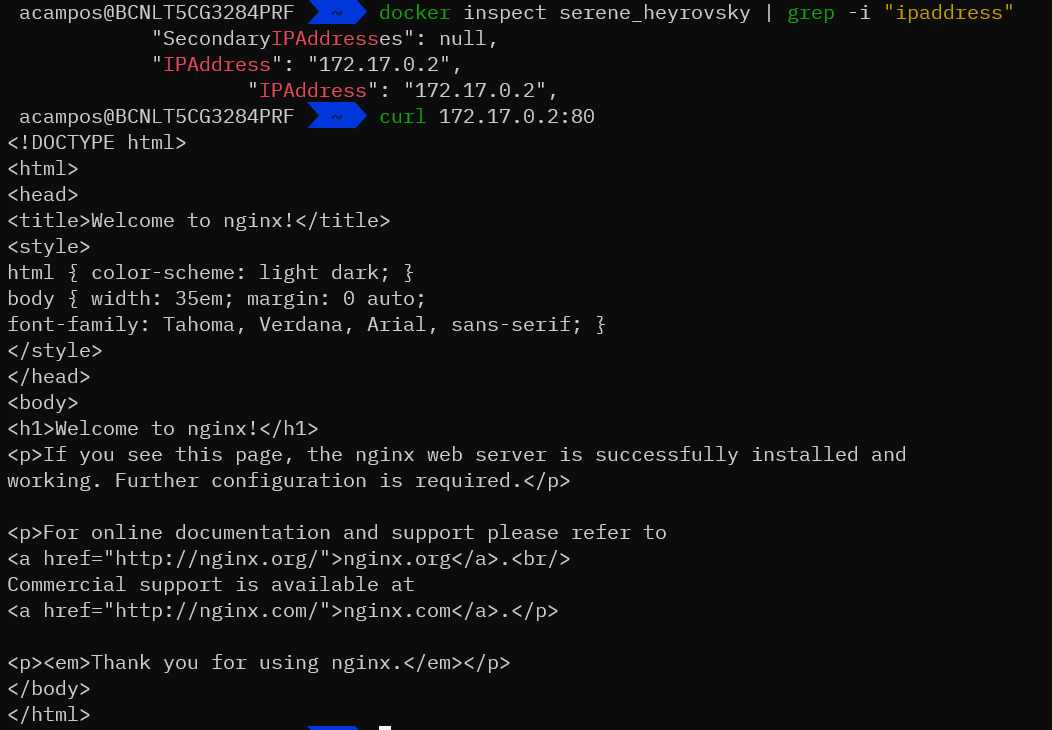
\includegraphics[scale=0.6]{pictures/imageNG.png}
\end{figure}

We can specify on the docker command a \textbf{NAT Rule}:
\begin{codetemplate}{}
\begin{verbatim}
$ docker run ... -p <host_port>:<container_port>
\end{verbatim}
\end{codetemplate}

That's the only way to make the application available to the outside world. Docker is automatically creating a NAT rule for that using the IP tables.

\subsection{CNI (Container Networking Interface)}

As we have seen in the previous section, isolate container Network is so hard, and this task is carried out by every software of containerization like: docker, rkt, mesos, K8s. All of them \textbf{associate containers to a Bridge Network (Namespace)} using the Bridges and IP / Routing isolation concepts we saw in the previous section.

So, someone smart, thought to externalize the functionality, and create a binary called \textbf{bridge} which creates an isolated Namespaces automatically with only one command. This binary is used by K8s, docker, mesos, etc. When a container starts, the binary is executed to create a Bridge Network (Namespace) where the container will run.

But this program is not closed, it has some configurations for the user to configure its own custom networks. That's where CNI (Container Network Interfaces) comes in. CNI is a set of standards that define how programs have to be defined to solve networking challenges in a container runtime environments. The programs are referred to as plugins, Bridge program is a plugin for CNI.

CNI defines a set of responsabilities  for container runtimes and pluggins. All the container manage systems can use these CNI's to define their networks, except Docker. 
\textbf{Docker does not implement CNI}, Docker has its own set of standards known as CNM which stands for container network model which is another standard similar to CNI but with some differences.

So when K8s run a docker container it runs it with \textbf{non-Network} and then invokes the configured CNI plugins who take care of the rest of the configuration

\subsection{Networking Cluster Nodes}

The K8s Cluster consists of Master and Worker Nodes, each node must have at least one interface connected to a Network and each interface must have an address configured. The hosts must have a unique host name set, as well as a unique MAC adress.

\begin{figure}[H]
    \centering
    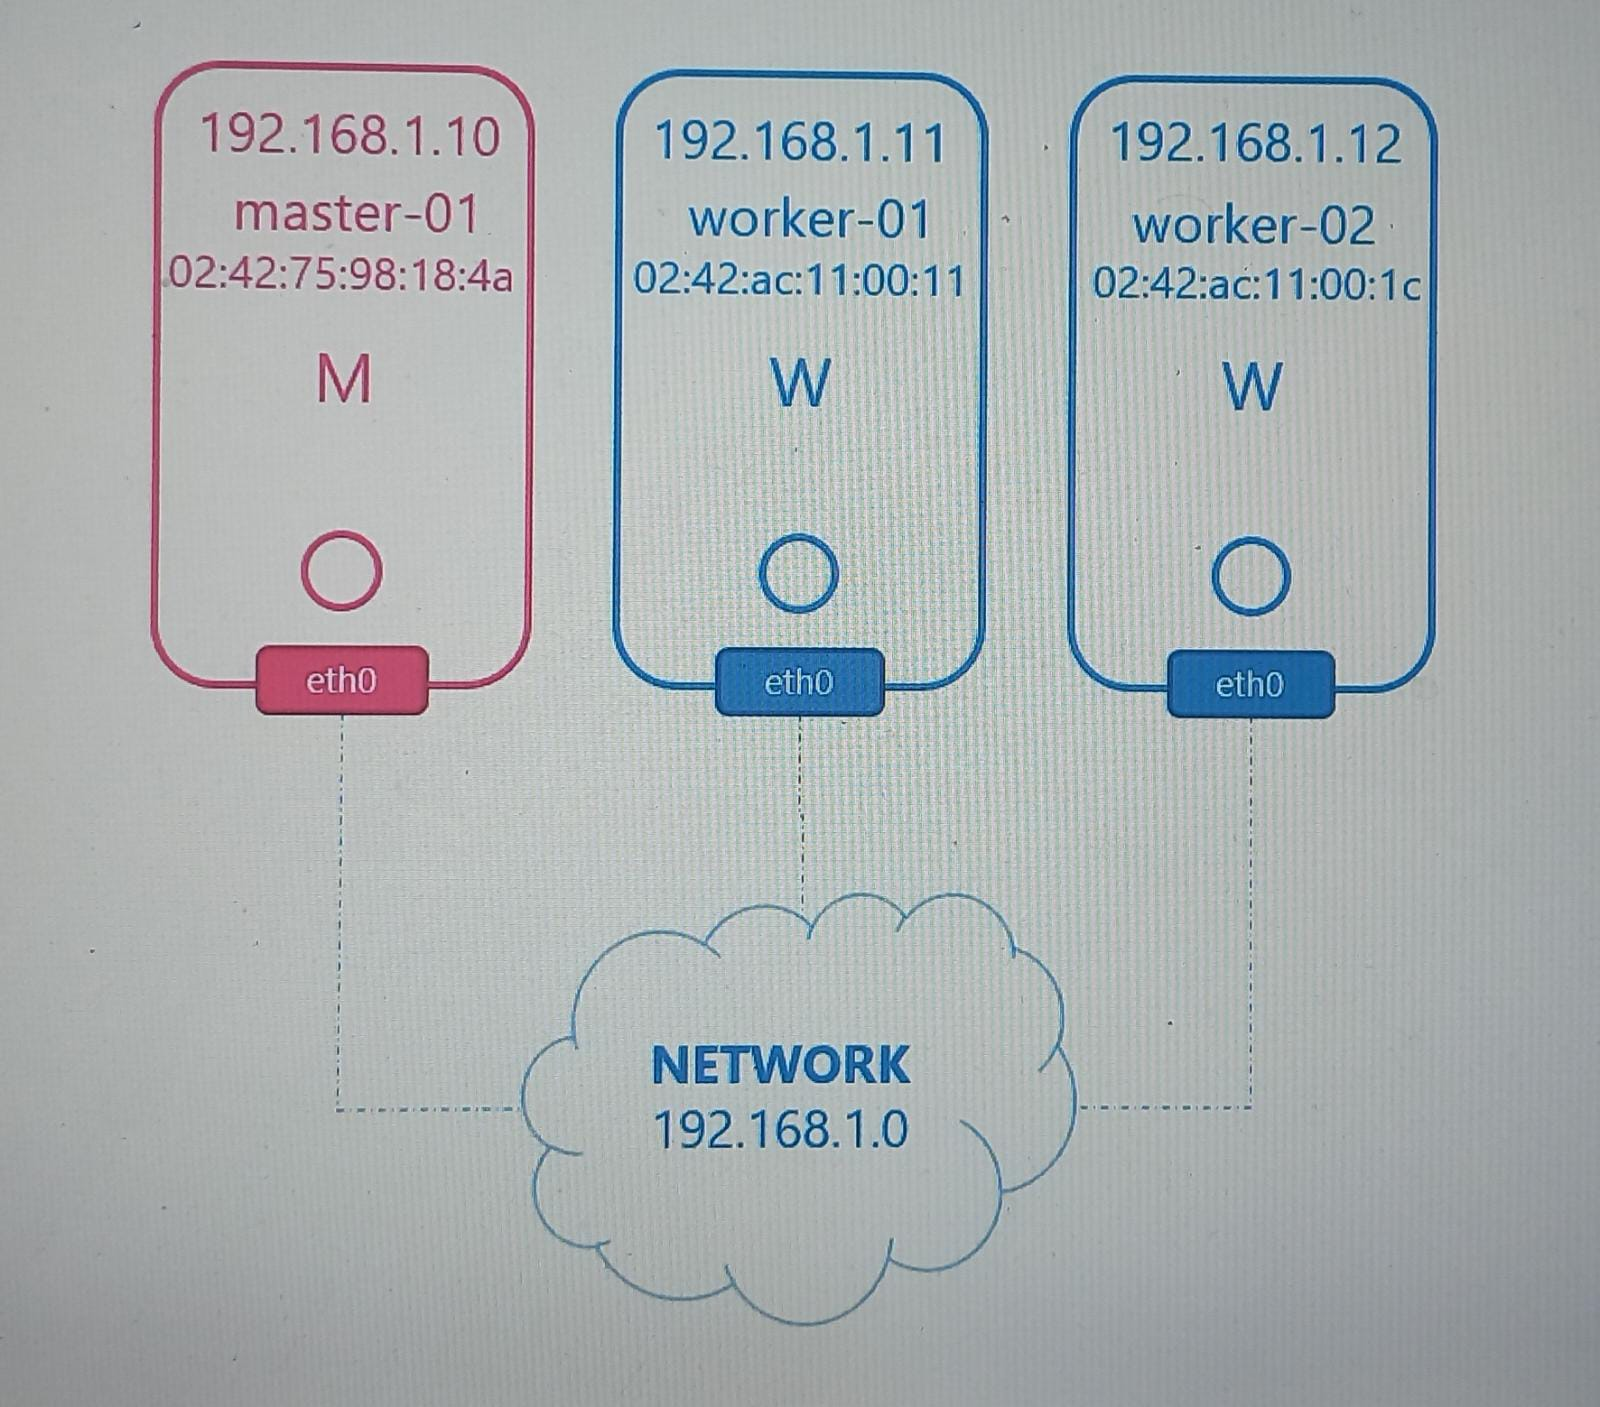
\includegraphics[scale=0.2]{pictures/locura1.png}
\end{figure}

Also, the Nodes must have the following ports opened:

\underline{Worker Nodes}
\begin{itemize}
    \item \textbf{10250:} kubelet
    \item \textbf{30.000 - 32.767:} services
\end{itemize}

\underline{Master Node}
\begin{itemize}
    \item \textbf{6443:} Kube-apiserver
    \item \textbf{10250:} kubelet
    \item \textbf{10251:} Kube-scheduler
    \item \textbf{10252:} Kube-controller-manager
    \item \textbf{2379:} etcd-cluster
\end{itemize}

\begin{figure}[H]
    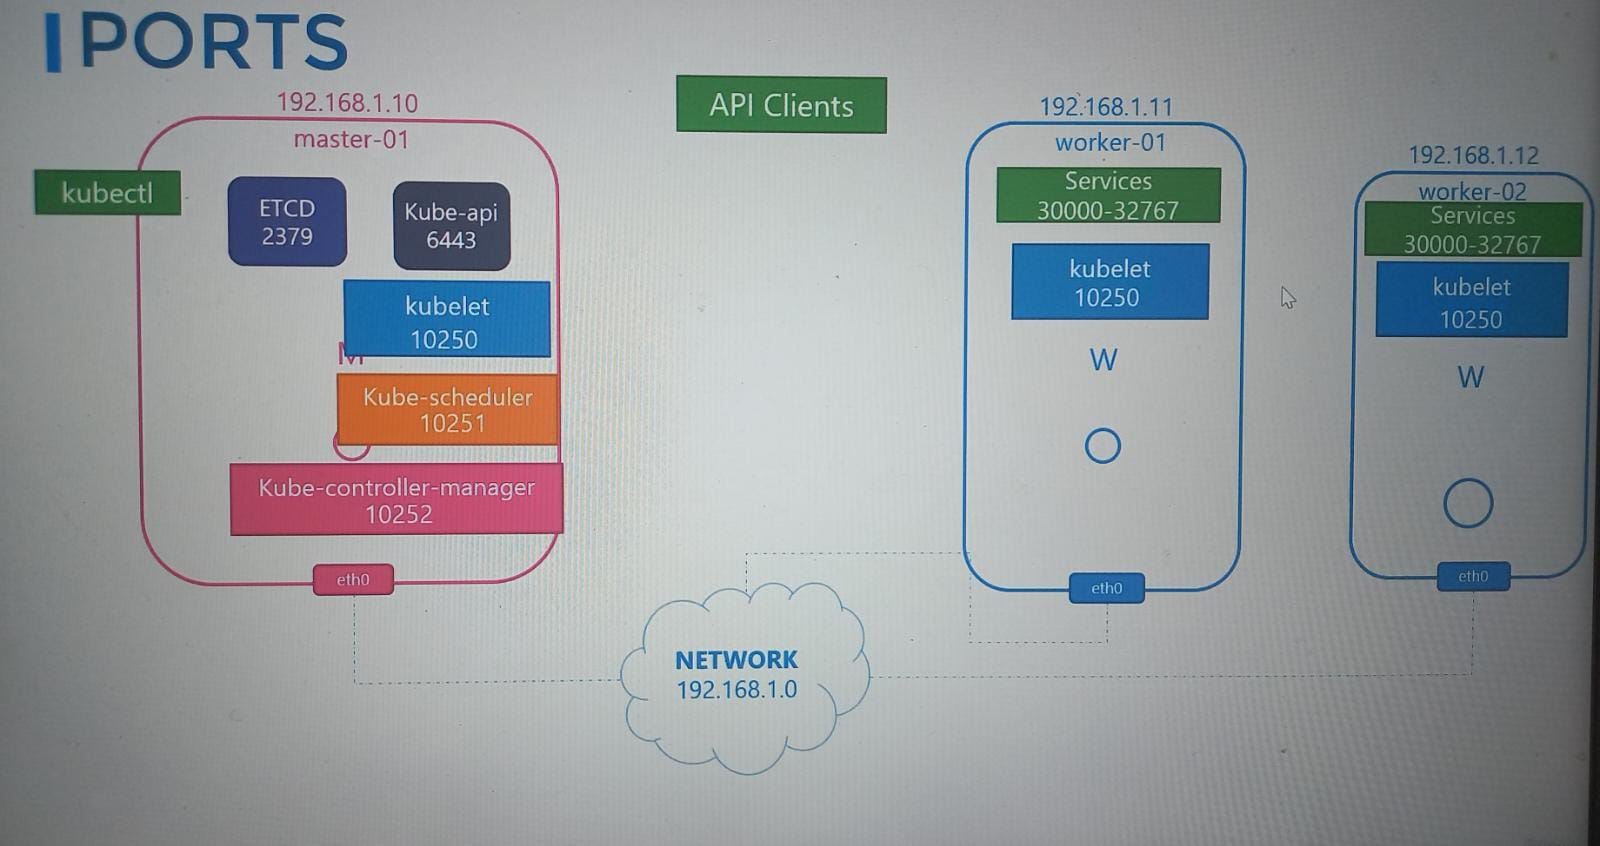
\includegraphics[width=\textwidth]{pictures/ports.png}
\end{figure}

\begin{blocktemplate}{NOTE}
Yes, a kubelet can be present on the Master Node. An if we have multiple Master Nodes (control-plane Nodes) all these ports need to be open those as well, and also need a \textbf{port 2380} to connect both \textbf{etcd-clients}
\end{blocktemplate}

\subsubsection{Useful Commands}

\begin{codetemplate}{}
\begin{verbatim}
$ ip link
\end{verbatim}
\end{codetemplate}

\begin{codetemplate}{}
\begin{verbatim}
$ ip addr
\end{verbatim}
\end{codetemplate}

\begin{codetemplate}{}
\begin{verbatim}
$ ip addr add 192.168.1.10/24 dev eth0
\end{verbatim}
\end{codetemplate}

\begin{codetemplate}{}
\begin{verbatim}
$ ip route
\end{verbatim}
\end{codetemplate}

\begin{codetemplate}{}
\begin{verbatim}
$ ip route add 192.168.1.0/24 via 192.168.2.1
\end{verbatim}
\end{codetemplate}

\begin{codetemplate}{}
\begin{verbatim}
$ ip route add deault via 192.168.2.1
\end{verbatim}
\end{codetemplate}

\begin{codetemplate}{}
\begin{verbatim}
$ cat /proc/sys/net/ipv4/ip_forward
> 1
\end{verbatim}
\end{codetemplate}

\begin{codetemplate}{}
\begin{verbatim}
$ arp
\end{verbatim}
\end{codetemplate}

\begin{blocktemplateII}{NOTE}
The ARP (Address Resolution Protocol) table is a crucial component of network communication, specifically within local networks. It functions as a mapping between IP addresses (logical addresses used in Layer 3 of the OSI model) and MAC addresses (physical hardware addresses used in Layer 2).
\\\\
When devices on a network communicate, data is transmitted using MAC addresses at the hardware level. However, applications and services use IP addresses. The ARP table helps bridge this gap by maintaining a lookup table that translates an IP address into the corresponding MAC address of a device within the same local network.
\end{blocktemplateII}

\begin{codetemplate}{}
\begin{verbatim}
$ netstat -plnt
\end{verbatim}
\end{codetemplate}

\subsection{POD Networking Concepts}

As we have seen, Master and Worker Nodes are configured to share the same Network, so they can reach each other. We also made sure the firewall and network security groups are configured correctly to allow for the K8s control plane components to reach each other. Supposing we have also set up all the K8s control plane components such as the kube-apiserver, etcd servers, kubelets, etc. Before applications can run, there is something that we must adress. We have talked about the Network that connects the Nodes,  but there is also another layer of networking that is crucial to the clusters functioning, and that is the networking at the Pod layer. Our K8s cluster is soon going to have a large number of Pods and services running on it, how are the Pods adressed? How do they communicate eachother? Internally inside the cluster and externally outside the cluster?

These are challenges that K8s expects we to solve, as of today, K8s do not come with a built-in solution for this. It expects we to implement a Networking Solution that solves this challenges. Nevertheless, K8s have laid out clearly the requirements for Pod Networking:

\begin{itemize}
    \item Every Pod should have a unique IP Adress. It does not care what IP address or what range or subnet it belongs to.
    \item Every Pod should be able to communicate with every other Pod on the same node.
    \item Every Pod should be able to communicate with every other Pod on other nodes without NAT.
\end{itemize}

So we need to provide a solution which automatically accomplish all these requirements. There are many solutions available, but all of them are based on the following concepts.

\begin{enumerate}
    \item When containers are created on the nodes, K8s creates Network Namespaces for them as docker, to enable communication between them we should attach these namespaces to a network, but which network?
    \item We create a virtual network on each node and bring them up:
\begin{codetemplate}{}
\begin{verbatim}
$ ip link add v-net-0 type bridge
\end{verbatim}
\end{codetemplate}
\begin{codetemplate}{}
\begin{verbatim}
$ ip link set dev v-net-0 up
\end{verbatim}
\end{codetemplate}

    \item We attach IP addresses to the bridges interfaces, each one in a subnetwork
\begin{codetemplate}{}
\begin{verbatim}
$ ip addr add 10.244.1.1/24 dev v-net # 10.244.2.1/24 and 10.244.3.1/24
\end{verbatim}
\end{codetemplate}

    \item When containers are created, then we need to attach them to the bridge using \verb|veth| (virtual ethernets) as we saw on the previous sections.
    \item Then we need to assign an IP to the container inside the subnet, which will be the following available inside the subnet, depending on the subnet:
    \begin{itemize}
        \item 10.244.1.2
        \item 10.244.2.2
        \item 10.244.3.2
    \end{itemize}
    \item Finally bring up the container network interface as we saw before.
\end{enumerate}

Whenever a new container is created, the last steps are repeated so all the containers are attached to the bridges inside their own nodes, with a unique IP address inside this network. So we have the 2 first conditions accomplished:
\begin{itemize}
    \item Pods (containers its the same on this case) has its own unique IP.
    \item Pods can communicate with other Pods inside the same node.
\end{itemize}

To enable connection between different nodes Pods, we need configure all the gateways on the nodes for all the Pods. Whenever we create a new Pod, we need to create on all the hosts a gateway to forward the traffic:
\begin{codetemplate}{}
\begin{verbatim}
node01$ ip route add 10.244.2.2 via <node_where_pod_running_ip>
\end{verbatim}
\end{codetemplate}

But as we can see, this is a lot of work. One better approach can be to configure a route table on a router if we have one in our network to avoid configure one by one all the pods gateways in all the nodes. So we just need to configure this router as default gateway.
As well, this actions are not done manually, we have the \textbf{CNI (Container Network Interface)}, which tells K8s what to do when creating a container. It is basically a script with the following sections:
\begin{itemize}
    \item \textbf{ADD:} adding a container interface to the network.
    \item \textbf{DEL:} deleting container interfaces from the network freeing the IP address.
\end{itemize}

So, when a container is created on K8s, the \textbf{container runtime} on each node is responsible for creating containers. It looks on CNI configuration:
\begin{codetemplate}{}
\begin{verbatim}
/etc/cni/net.d/net-script.conflist
\end{verbatim}
\end{codetemplate} 

And identifies our script's name, looking for it:
\begin{codetemplate}{}
\begin{verbatim}
/opt/cni/bin/net-script.sh
\end{verbatim}
\end{codetemplate} 

And then executes it:
\begin{codetemplate}{}
\begin{verbatim}
./opt/cni/bin/net-script.sh add <container> <namespace>
\end{verbatim}
\end{codetemplate} 

\subsection{CNI in K8s}
As we have seen, CNI (Container Network Interface) defines the responsibilitires of container runtime. But the responsible of creating the containers namespaces, attach this namespaces to teh bridge, etc. Is the K8s \textbf{container runtime}, wich commonly is one of this 2:
\begin{itemize}
    \item \textbf{containerd}
    \item \textbf{cri-o}
\end{itemize}

First of all, all the Network Plugins should be installed on the following folder because it is where the container
runtimes are going to look for the plugins:
\begin{codetemplate}{}
\begin{verbatim}
/opt/cni/bin/
\end{verbatim}
\end{codetemplate}

But which plugins to use is configured on:
\begin{codetemplate}{}
\begin{verbatim}
/etc/cni/ned.d/flannel.conflist 
\end{verbatim}
\end{codetemplate}
\begin{codetemplate}{}
\begin{verbatim}
/etc/cni/ned.d/bridge.conflist 
\end{verbatim}
\end{codetemplate}

\subsection{WeaveWorks Wearks CNI Plugin}
\subsubsection{How does it work?}
WeaveWorks is a solution based on CNI, so instead of our own script, we integrated the weave plugin. 
In a 3 nodes cluster, with a router which has IP in the same pod network, we have an ip table with all the information of how to redirect all the traffic depending on the IP. Can be a good solution, but for many nodes and hundreds of thousands of pods, because the routing table won't support as many entries... It is not pratical.

So we need to imagine all the K8s Cluster as a company, the different Nodes are offices, namespaces are deparments and pods are directly people. So \textbf{WeaveWorks} will be the delivery company transporting packages from one person in one office to other person into another office. The first think that the
delivery company do (\textbf{WeaveWorks}) is place one agent on each office (node). These agents are responsible for managing all shipping activities between sites, they keep talking to each other every time and are well connected.

So the thing is, whenever a Pod send a package this agent intercepts it, ask to other agents if they have the IP where the Pod wants to connect and then it sends the package to the agent answering, yes I have this pod, send it to this direction. Then, the receiver agent intercepts the package and delivers it to the right Pod.

If we are asking, yes, the agents have their own private network to connect each other, an then another network interface to contact with the Pods.

\subsubsection{How to deploy Weave on a K8s Cluster?}
They can be deployed as services or deamons (with daemonset) on each node in the cluster manually.

Here is the way to deploy \textbf{weave} as daemons with daemonset:
\begin{codetemplate}{}
\begin{verbatim}
$ kubectl apply -f \
 "https://cloud.weave.works/k8s/net?k8s-version=$(kubectl version | base64 | tr -d '\n')"
\end{verbatim}
\end{codetemplate}

It will deploy:
\begin{itemize}
    \item ServiceAccount
    \item ClusterRole
    \item ClusterRoleBinding
    \item Role
    \item RoleBinding
    \item One daemon on each node on the cluster
\end{itemize}

\begin{figure}[H]
    \centering
    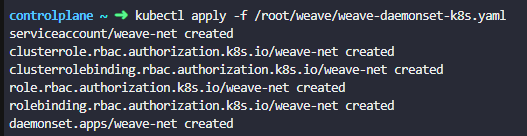
\includegraphics[width=\textwidth]{pictures/weave.png}
\end{figure}

\subsection{Other Network K8s Plugins}

There are other Network K8s Solutions (plugins), like:
\begin{itemize}
    \item \textbf{Calico:} the most popular and widely adopted networking solutions for Kubernetes. It provides scalable, high-performance, and secure networking and network policy enforcement. It supports both layer 3 (L3) routing and layer 2 (L2) switching.
    \item \textbf{Flannel:} simple and easy-to-use network overlay solution designed specifically for Kubernetes. It primarily provides L3 networking and is often used as a default for Kubernetes clusters.
    \item \textbf{Cilium:}  advanced networking plugin built on eBPF (extended Berkeley Packet Filter), which allows dynamic, programmable networking. It is designed for securing and observing network traffic in microservices architectures.
    \item \textbf{Contiv:}  robust CNI plugin that provides a rich set of features for networking and security. It supports both Kubernetes and Docker Swarm, making it versatile for containerized environments.
    \item \textbf{Kube-router:} lean, simple, and high-performance network plugin designed to handle both networking and network security for Kubernetes clusters. It integrates BGP (Border Gateway Protocol) for routing between nodes..
    \item ...
\end{itemize}

\subsection{IPAM (CNI)}
IP Address Management, so how does it work on K8s? How does K8s assing virtual IP's from the nodes to a virtual subnet? And how the Pods as well assigned an IP?

CNI says it is responsability of the CNI plugin the network solution provider to take care of assigning IP's to the containers. The K8s does not care about how we do it, we just need to do it, but making sure we don't assign any duplicate IP's. But instead of doing it manually, the CNI comes with two built-in plugins to perform this task:
\begin{itemize}
    \item DHCP
    \item host-local
\end{itemize}

So we need to choose which one of them inside:
\begin{codetemplate}{}
\begin{verbatim}
/etc/cni/ned.d/...
\end{verbatim}
\end{codetemplate}

Each plugin (like weaveworks) has its own solution for that. For example, weaveworks.
\begin{itemize}
    \item Ip range 10.32.0.0/12 (10.32.0.1 - 10.47.255.254). So 1.0048.574 Pods and nodes!
    \item To the nodes it assign subnetworks like (10.32.0.1, 10.38.0.0, 10.44.0.0).
    \item Pods created will have IP's on the node network range.
\end{itemize}

\subsection{Service Networking}

\subsubsection{Introduction}
In previous section we have talked about Pods Networking, how bridge networks are created within each node and how pods get a namspace created for them, and how interfaces are attached to those namespaces, and how Pods get an IP adress assigned to them within the subnet assigned for that Node.

We also saw through routes, we can get the Pods on different Nodes to talk to each other forming a large Virtual Network where all Pods can reach each other. But it is so rare to configure Pods to communicate directly with each other (todo este rollazo para nada, diosmio). \textbf{Normally, when we want a Pod to access apps hosted on another Pod we would always use a Service object.}

So, if a Pod wants to consume an app, it only have to use the IP assigned to its Service or the Service name. It does not matter if it a Pod from the same Node, because when a Service is created it is accessible from all Pods on the Cluster. Because a Service is hosted across the cluster, not bound to a specific Node. 

\begin{blocktemplateIII}{WARNING}
All the Services are accessible by each resource inside the cluster by its name or its IP, but it is not accessible from outside the Cluster, because its IP belongs only to the Virtual Internal Network of K8s    
\end{blocktemplateIII}

The more basic Service configuration is of type \textbf{ClusterIP}. \textbf{NodePort} does exactly the same as \textbf{ClusterIP} Service but in addition, it exposes the application on a port on all Nodes in the Cluster. This way, external users can use the service connecting directly with nodes IP's.

\subsubsection{How services works, kube-proxy}

So our focus must be more on Services than in Pods, how are these Services getting these IP addresses? And how are they made available across all the Nodes in the Cluster? How is the service made available to external users throuhg a port on each Node? The responsible is \textbf{kube-proxy} element, which is running into every Node on the Cluster.

\textbf{Kube-proxy} element watches the changes in the cluster through kube-apiserver and every time a new service is to be created, kube-proxy gets into action. Unlike Pods, Services are not created on each Node or assigned to a Node, \textbf{Services are Cluster-wide concept}. They exists across all the Nodes in the Cluster. As a matter of fact, they do not exist at all. Besides, there are no processes, bridges, namespaces or interfaces for a Service, it is just a virtual object. 

So how do they get an IP adress? And how are we able to access the application on a Pod through a Service? \textbf{When we create a service object in K8s it is assigned an IP address from a predefined range}. The \textbf{kube-proxy} components running on each node gets that IP address and creates forwarding rules on each Node saying: "Any traffic comming to this IP should go to the IP of the Pod". Once that is in place, whenever a pod tries to reach the IP of the Service it is forwarded to the Pod's IP address, which is accessible from any Node in the Cluster (as we have discussed in previous sections). But remember, it is not just an IP, it is an IP and a Port combination, whenever Services are created or deleted \textbf{kube-proxy} component of each Node creates or delete these rules.

\subsubsection{How kube-proxy set that rules?}

kube-proxy supports different ways to set networking rules:

\begin{itemize}
    \item \textbf{userspace:} kube-proxy listens on a port
    \item \textbf{ipvs rules}
    \item \textbf{iptables (default):} as we saw in section \ref{swrt}
\end{itemize}

The kube-proxy can be set using the proxy mode option, default is iptables:

\begin{codetemplate}{}
\begin{verbatim}
$ kube-proxy --proxy-mode [userspace | iptables | ipvs] ...
\end{verbatim}
\end{codetemplate}

\subsubsection{Example of iptable rule application}
\begin{itemize}
    \item Pod running on IP 10.244.1.2
    \item Service with ClusterIP 10.134.132.104, ports 3306:3306
\end{itemize}

When the service is created K8s cluster assigns a predefined IP to it (ClusterIP), just reachable from the Pod Network. The range of address that K8s can assign is defined on \textbf{kube-apiserver} configuration. By default it is \textbf{10.0.0.0/24}:
\begin{codetemplate}{}
\begin{verbatim}
--service-cluster-ip-range
\end{verbatim}
\end{codetemplate} 

To inspect the NAT rules created by the \textbf{kube-proxy} on all the nodes:
\begin{codetemplate}{}
\begin{verbatim}
$ iptables -L -t nat | grep -i <service_name>
\end{verbatim}
\end{codetemplate}

On the logs of \textbf{kube-proxy} as well we will see which proxier it uses (commonly iptables). As well we will see the rule whenever we create a new service:
\begin{codetemplate}{}
\begin{verbatim}
$ kubectl logs -n kube-system kube-proxy-84pj7
\end{verbatim}
\end{codetemplate}
\begin{codetemplate}{}
\begin{verbatim}
$ tail /var/logs/kube-proxy.log
\end{verbatim}
\end{codetemplate}

\subsection{DNS on K8s}
\subsubsection{Introduction}
So imagine we have 3 Nodes in our K8s cluster with Pods and services running. 
Each node has a nodename and IP adress assignet to it. 
The Node names and IP adresses  of the Cluster are probably registered in
DNS servers in our organization, and how access them are not of concern in this section, in this section we will discuss the DNS resolution within the cluster, between different components such as Pods and Services.

K8s deploys a \textbf{built-in DNS server} by default when we setup a cluster, if we run k8s from scratch, we have to do it by yourself. We focus purely on pods and services within the cluster, we are not interested on Nodes FQDN. 

Let's se this example:

\begin{figure}[H]
    \centering
    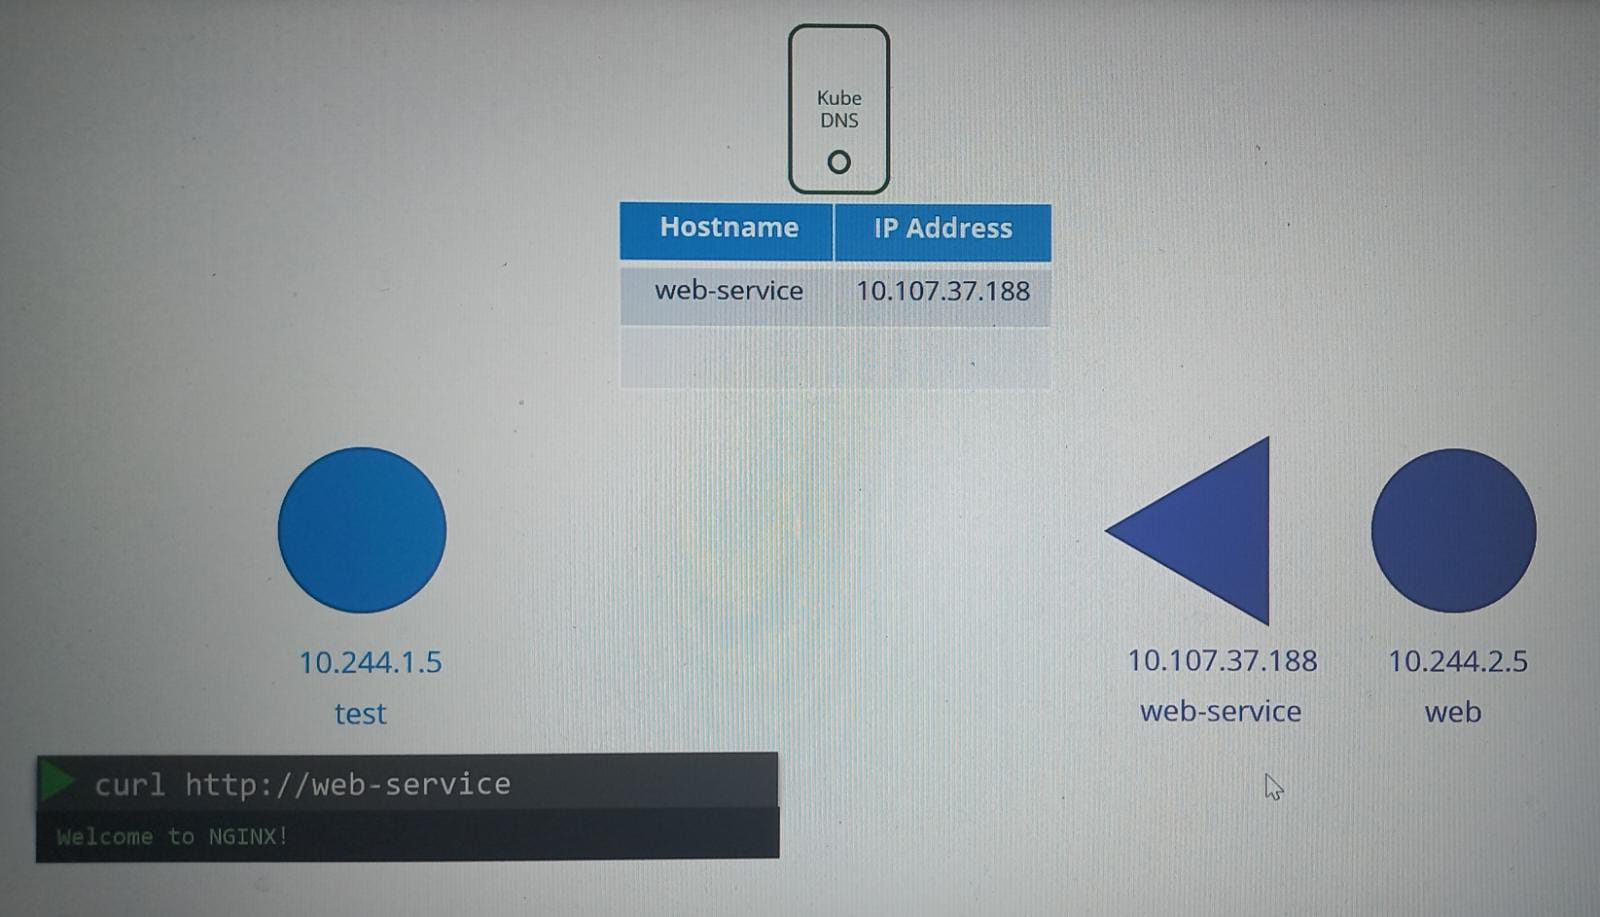
\includegraphics[width=\textwidth]{pictures/ingress1.png}
\end{figure}

Looking at the Pods IP's we should notice that it would be running on different Nodes,
but this is not important, because all Pods and Services can reach each other using 
their own IP addresses in their specific network. 
But this is not the best way to communicate between Pods, as we know, the best way is to use Services. The service IP? we can, but is better to do it using directly its FQDN.

Whenever a \textbf{Service} is created, the \textbf{K8s DNS Server creates a record for the Service, mapping the Service name with its IP address}. So within the Cluster, any Pod can reach now the newly created Service using its service name. \textbf{Remember that the Service name can change if the Pod who is calling it is in the same Namespace or in another Namespace}

\begin{itemize}
    \item \textbf{Pod in the same Namespace:} \verb|service_name|
    \item \textbf{Pod outside the Service Namespaces:} \verb|service_name.namespace_name|
\end{itemize}

Whenever a Namespace is created, \textbf{K8s DNS Server} creates a Sub domain for this namespace. 


\begin{blocktemplate}{NOTE}
However, we can reach the Service as well on this FQDN's:
\begin{itemize}
    \item \verb|service_name.namespace_name.svc|
    \item \verb|sservice_name.namespace_name.svc.cluster.local|
\end{itemize}

This is because all the Services are grouped together into another Sub Domain called \textbf{svc}, 
so we can reach our application using the FQDN: \verb|service_name.namespace_name.svc|. 
\\\\
Additionally, Services and Pods are grouped together into another Sub Domain: \textbf{cluster.local}, 
so we can also reach our application using the FQDN:
\verb|service_name.namespace_name.svc.cluster.local|.
\end{blocktemplate}

Records for Pods \textbf{are not created by default, but we can enable that explicitly}. 
If we enabled it, whenever a Pod is created the \textbf{K8s DNS Server} will create 
a record for the Pod, which won't be the Pod name, it will be exactly equal to the IP 
of the Pod but with dashes (\verb|10.3.4.0 : 10-3-4-0|). 
The \textbf{Namespace} will be the same and type will be pod. So their FQDN will be: 
\begin{codetemplate}{}
\begin{verbatim}
pod_ip_dashes.namespace_name.pod.cluster.local
\end{verbatim}
\end{codetemplate}

\begin{blocktemplateIII}{WARNING}
I don't know why but for pods the only available FQDN is: \verb|pod_ip_dashes.namespace_name.pod.cluster.local|
\end{blocktemplateIII}

\subsubsection{How K8s Implements DNS in the Cluster}
How K8s makes possible to reach a Service or a Pod from another Pod using an FQDN? So if we have 2 or 3 Pods, we only have to configure the \verb|/etc/hosts| file to add the mapping. But as in a Cluster can be thousands of hundreds of Pods it is not feasible. Instead we move these entries into a \textbf{Central K8s DNS Server}. We have to add this \textbf{DNS Server} to the Pods configuration file \verb|/etc/resolv.conf| specifing that the nameserver is at the IP address of the \textbf{Central K8s DNS Server}. Every time a new Pod or Service is created we add a record in the DNS server for that Pod so the other Pods can access the new Pod or Service with their FQDN, and the new Pod can also resolve other Pods in the Cluster.

\begin{figure}[H]
    \centering
    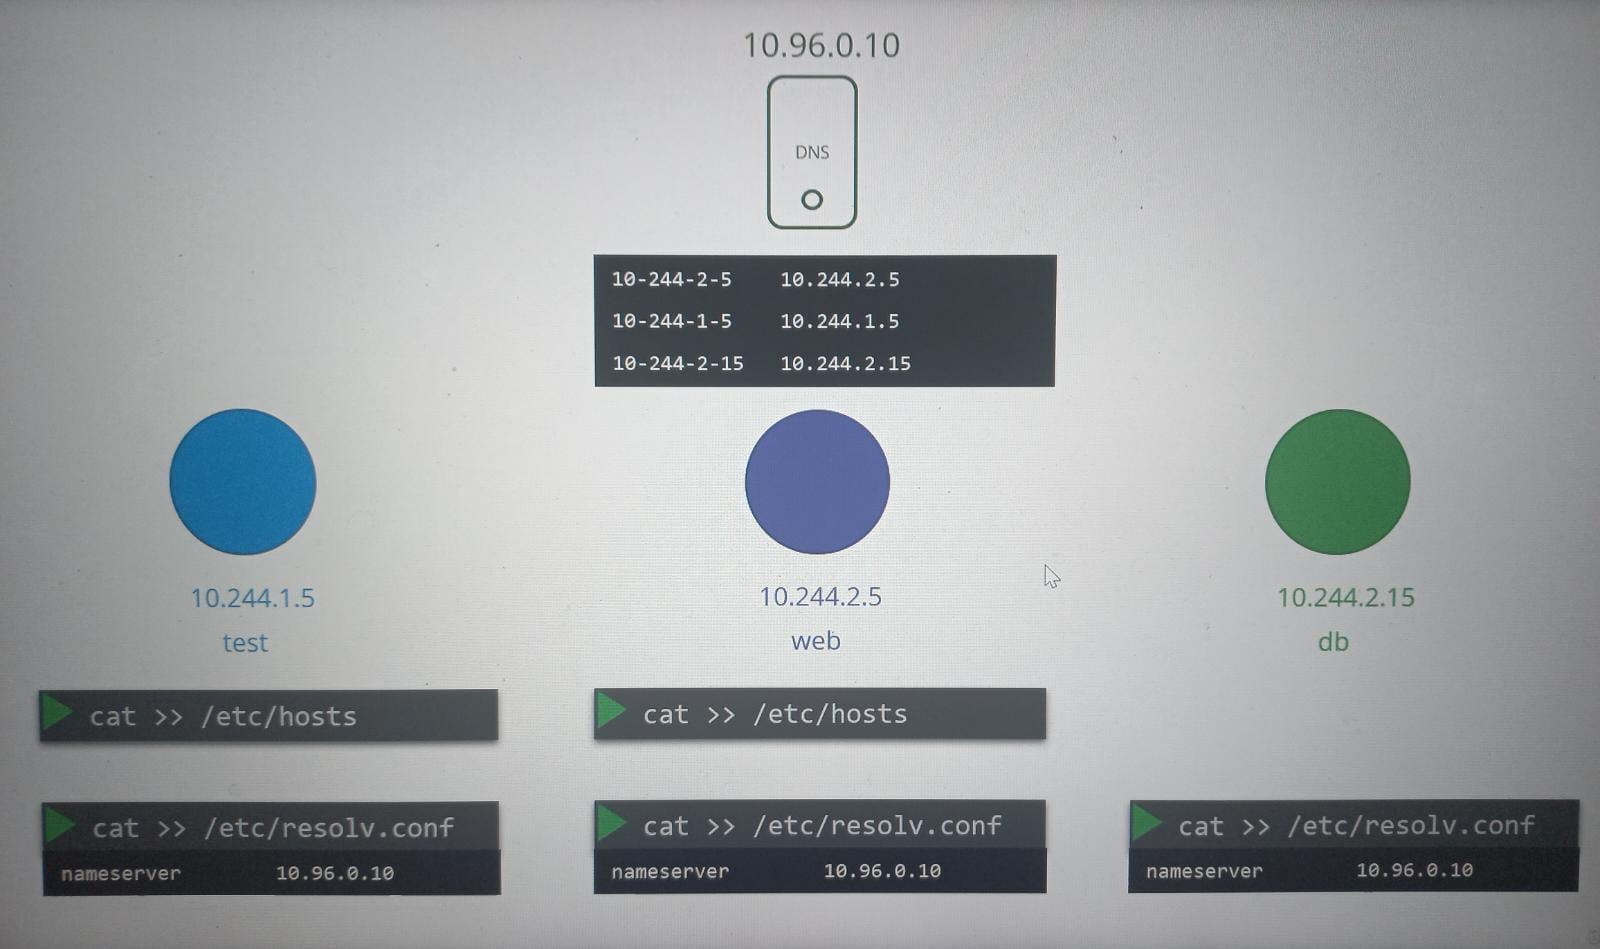
\includegraphics[width=\textwidth]{pictures/ingress2.png}
\end{figure}

K8s implement DNS in the same way, it deploys a \textbf{DNS Server} within the Cluster, it must be CoreDNS. But how is CoreDNS setup in the Cluster. It is deployed as a Pod in the \textbf{kube-system Namespace}, actually it is created as two Pods for redundancy as par of a ReplicaSet and a Deployment. This Pod runs \textbf{CoreDNs executable} the same executable we should run if we create our cluster from scratch. It requires a configuration file named Corefiled located on \verb|/etc/coredns/Corefile|

\begin{figure}[H]
    \centering
    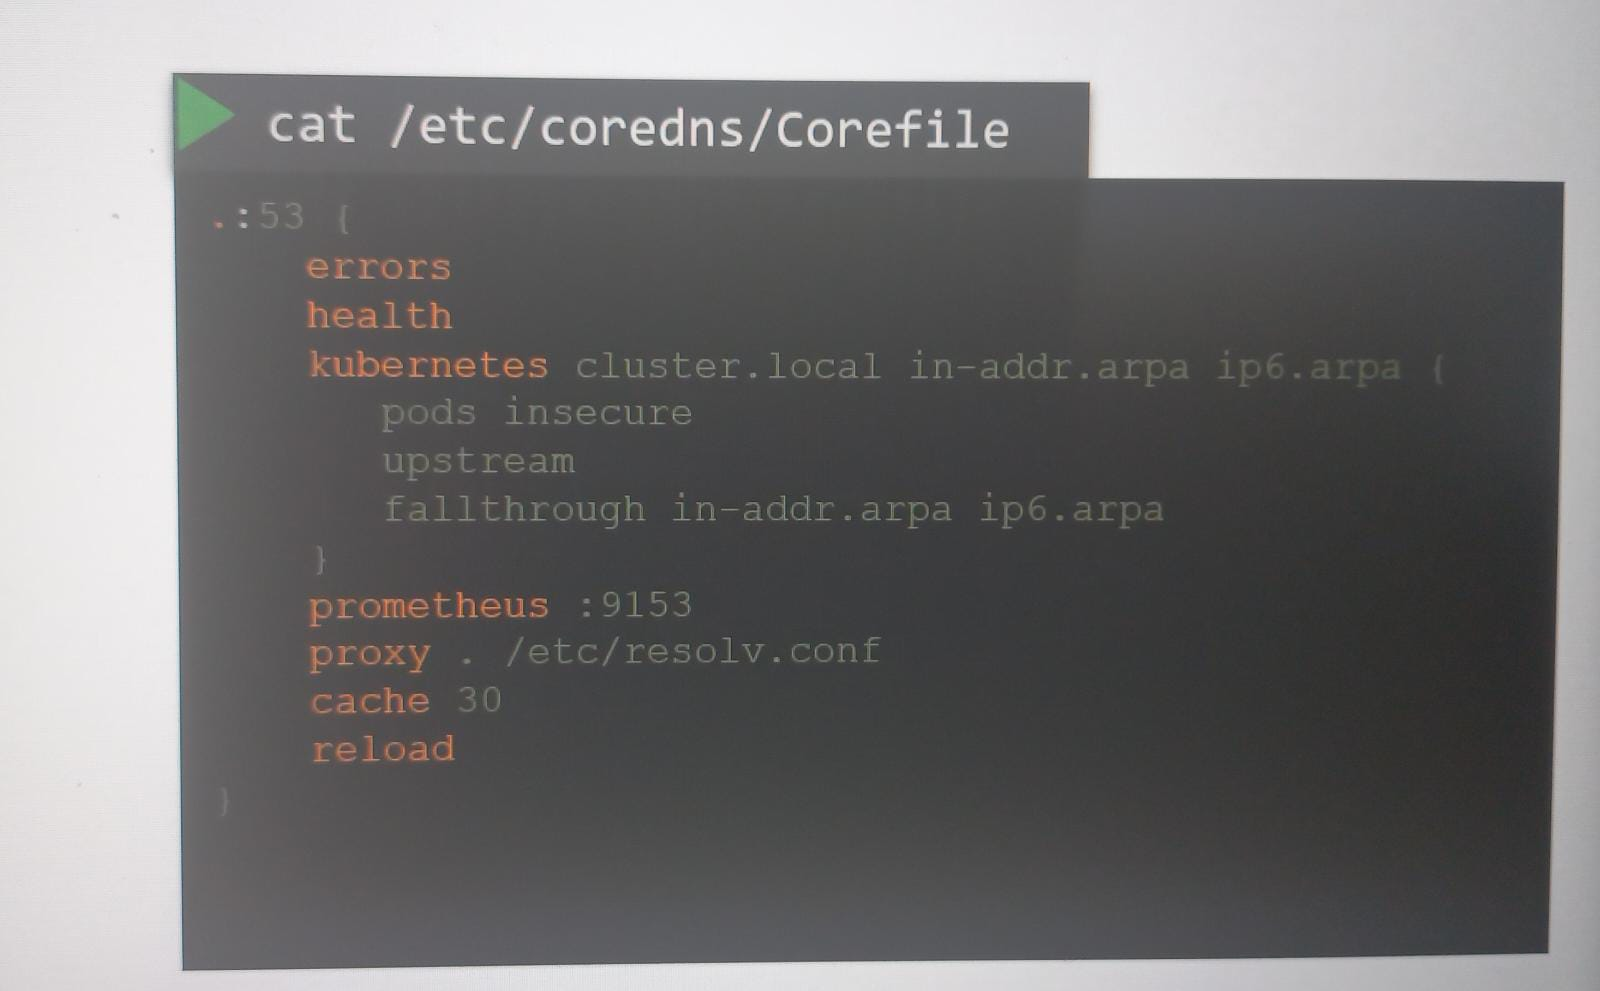
\includegraphics[scale=0.2]{pictures/ingress3.png}
\end{figure}

This file is charged into a \textbf{ConfigMap in the K8s kube-admin Namespace}. When \textbf{CoreDNS} por is up and running using the appropiate K8s plugin, 
it watches the K8s Cluster for new Pods or Services, and every time a Pod or a Service is created, 
it adds a records for it in its database.

\subsubsection{How Pods point to the CoreDNS Server?}

What adress do the Pods use to reach the \textbf{DNS Server}?
What address do the Pods use to reach the DNS server? So when we deploy the CoreDNS solution it
also creates a service to make it available to other components within the cluster,
its name is by default \textbf{kube-dns}.

K8s automatically configure the \textbf{kube-dns} service IP into the \verb|/etc/resolv.conf| of the Pods when it creates them, we don't
have to configure anything by yourself. The responsible component of that task is \textbf{kubelet},
if we check at the kubelet configuration we will see the fields:

\begin{codetemplate}{}
\begin{verbatim}
clusterDNS:
- 10.96.0.10
clusterDomain: cluster.local
\end{verbatim}
\end{codetemplate}

\subsection{Ingress}

\href{https://kubernetes.io/docs/concepts/services-networking/ingress/}{Official K8s Doc}

\subsubsection{The need of Ingress}

Imagine we are deploying an application on K8s for a company that has an online store selling products, our application would be available at \verb|my-online-store.com|. 
You build our application:
\begin{itemize}
    \item \textbf{Main Application:} running inside a docker container, inside a Pod, managed by a Deployment and accessible from inside the cluster through a service.
    \item \textbf{MySQL db:} running inside a docker container, inside a Pod, managed by a Deployment and accessible from inside the cluster through a service.
\end{itemize}

The main application can easily access the mysql database as we know using \verb|service_name| (because they are in the same namespace), 
\textbf{but how can we make the application accessible to the outside world?}. For now it is only accessible from inside the cluster using the service IP or FQDN.

And in the following example, just in the case the service is \textbf{NodePort} type, the application may be
accessible on \verb|http://IP_OF_ONE_RANDOM_NODE:38080.| And as well we can onfigure our DNS Server to point to the IP of the Nodes and FQDN so the users can now access the application using the URL \verb+http://my-online-store.com:38080+.

\begin{figure}[H]
    \centering
    \includegraphics[width=\textwidth]{pictures/ingress4.png}
\end{figure}

But if the service is from another type, we won't be able to do that. As well, we don't want to have a lot of application running on ports of the Nodes directly, it is not a good approach, because if they need to be accessible
using TLS (https) they need to be exposed on 443. So we need to think about another solution.
As well if our company grows and we now have new services for our customers, 
for example, a video streaming service. 
Now we want our users to be able to access our new video 
streaming service by going to my-\textbf{online-store.com/watch} and we want our old application
be accessible now at \textbf{online-store.com/wear}. 
But they are actually two different microservices or directly applications.
So we deploy our new application as a separate Pod, Deployment and Service.

You can create another LoadBalancer with a new IP (remember that we must pay for each of these load balancers)
and having many such loadBalancers can inversely affect our Cloud Bill.
As well we need yet another proxy or LoadBalancer that can redirect traffic based on URL to the different Services. 
And every time we introduce a new Service we have to reconfigure the LoadBalancer. In addtion, we should enable SSL for our applications so our users can access our application using https. 
Where do we configure that? It can bedone at different levels: 

\begin{itemize}
    \item Application Level
    \item Load Balancer Level
    \item Proxy Server Level
\end{itemize}

But we want to configure that in one place with minimal maintenance.

\begin{figure}[H]
    \centering
    \includegraphics[width=\textwidth]{pictures/ingress7.png}
\end{figure}

So when the Cluster scales it becomes unmanageable, it would be nice if K8s manage all of that within the K8s Cluster and have all that configuration in just another configuration file that lives along with the rest  of our application Deployment and Services files. And this exists and they are Ingress.

\subsubsection{Introduction to Ingress}

\textbf{Ingress} helps users to access our application using a single externally accessible URL that we can configure to route traffic to different services within our Cluster based on the URL path. At the same time, implement SSL security as well. Think of \textbf{Ingress} as a layer 7 LoadBalancer built in the K8s Cluster that can be configured using native K8s primitives just like any other Object.

Even with \textbf{Ingress} we still \textbf{need to expose it to make it accessible outside the Cluster}, so we still have to either \textbf{publish it as a NodePort or with a Cloud-native LoadBalancer}. But that is just a one-time configuration. Going forward, we are going to perform all our load balancing of SSL and URL-based routing configuration on the \textbf{Ingress-Controller}.

\subsubsection{Ingress Controller \& Ingress Resources}

But what is an Ingress? Where it is? How can we see it, and how can we configure it? Without Ingress all its works would be done with a proxy-reverse or a LoadBalancer like NGINX, HAproxy, etc. It will be deployed in the K8s Cluster and configure them to route traffic to another services, with user routes, SSL certificates, endpoint services, etc.

\textbf{Ingress} are implemented by K8s in a very similar way, the \textbf{product deployed} by K8s is called \textbf{Ingress Controller} (is a product like NGINX), and the \textbf{set of rules} we configure are called \textbf{Ingress Resources}. \textbf{Ingress Resources} are created using definition YAML files. 

\subsubsection{Ingress Controller}

K8s Clusters does not come with an Ingress Controller by default, 

There are a number of solutions available for \textbf{Ingress Controller:}
\begin{itemize}
    \item \textbf{GCE:} Google Controller layer 7 HTTP Load Balancer
    \item \textbf{NGINX}
    \item \textbf{Istio}
    \item \textbf{HAPROXY}
    \item \textbf{Treafic}
\end{itemize}

Currently, \textbf{GCE} and \textbf{NGINX} are currently being supported and maintained by the K8s project, and in this section we will use NGINX as an example. This Ingress Controller are not just another Load Balance or NGINX server, the Load Balancer components are just part of it. Ingress Controllers have additional \textbf{intelligence} to \textbf{monitor} the K8s Cluster for \textbf{new} definitions of \textbf{Ingress Resources} and configure the \textbf{NGINX Server accordingly}. A \textbf{NGINX Controller} is deployed just as another deployment in K8s.

To run \textbf{properly} an \textbf{Ingress Controller} in our K8s Clsuter we should \textbf{create} the following resources:

\begin{itemize}
    \item \textbf{Deployment} with an Ingress Controller Image to run into containers
    \item \textbf{ConfigMap} to configure the NGINX
    \item \textbf{Service} type NodePort to expose it
    \item \textbf{ServiceAccount} with the right permission to access all of these objects
\end{itemize}

\paragraph{Deployment}

\begin{codetemplate}{nginx-ingress-controller.yaml}
\begin{verbatim}
apiVersion: extensions/v1beta1
kind: Deployment
metadata:
    name: nignx-ingress-controller
spec:
    replicas: 1
    selector:
        matchLabels:
            name: nginx-ingress
    template:
        metadata:
            labels:
                name: nginx-ingress
        spec:
            containers:
            - image: quay.io/kubernetes-ingress-controller/nginx-ingress-controller:0.21.0
              name: nginx-ingress-controller
            args:
            - /nginx-ingress-controller
            - --configmaps=$(POD_NAMESPACE)/nginx-configuration
            env:
            - name: POD_NAME
              valueFrom:
                fieldRef:
                    fieldPath: metadata.name
            - name: POD_NAMESPACE
              valueFrom:
                fielRef:
                    fieldPath: metadata.namespace
            ports:
            - containerPort: 80
              name: http
            - containerPort: 443
              name: https
            
\end{verbatim}
\end{codetemplate}

Within the image, the NGINX program is stored at location \verb|/nginx-ingress-controller| so we must pass that as the command to start the NGINX controller service. Also, NGINX has more configurations like:
\begin{itemize}
    \item Path to store the logs
    \item Keep alive threshold
    \item SSL settings
    \item Session timeout
\end{itemize}

Also NGINX server need the env configuration to run properly and to specify the ports used by the Ingress Controller, which happens to be 80 for http connections and 443 for secure (https) connections.

\paragraph{ConfigMap}

In order to decouple this configuration data from the NGINX Controller Image we must create a ConfigMap Object:

\begin{codetemplate}{nginx-configuration.yaml}
\begin{verbatim}
apiVersion: v1
kind: ConfigMap
metadata:
    name: nginx-configuration
\end{verbatim}
\end{codetemplate}

You can let it blank if we want, it would apply the configuration by default, but it would make easy for we to modify a configuration setting in the future.

\paragraph{Service}
We then need a Service to expose the Ingress Controller to the external world, so we create a Service of type NodePort with the nginx-ingress label selector to link the service to the Deployment:

\begin{codetemplate}{}
\begin{verbatim}
apiVersion: v1
kind: Service
metadata:
    name: nginx-ingress
spec:
    type: NodePort
    ports:
    - port: 80
      targetPort: 80
      protocol: TCP
      name: http
    - port: 443
      targetPort: 443
      protocol: TCP
      name: https
    selector:
        name: nginx-ingress
\end{verbatim}
\end{codetemplate}

\paragraph{ServiceAccount}

As we said before, the Ingress Controllers have additional intelligente built into them to monitor the K8s Cluster for Ingress Resources and configure the underlying Ingress Controller when something is changed. But for the Ingress Controller to do this, it requires a Service Account with the right set of permissions: Roles, ClusterRoles and RoleBindings

\begin{codetemplate}{}
\begin{verbatim}
apiVersion: v1
kind: ServiceAccount
metadata:
    name: nginx-ingress-serviceaccount
\end{verbatim}
\end{codetemplate}

\subsubsection{Ingress Resources}

\href{https://kubernetes.io/docs/concepts/services-networking/ingress/}{Official K8s Doc}

An Ingress Resource is a set of rules and configurations applied on the \textbf{Ingress Controller}, we can configure rules to say simply forward all incoming traffic to a single application or route traffic to different applications based on URL, so if the user  goes to my-online-store.com/wear then route to one app, or if the user visits the my-online-store.com/watch then route to another app. Or we can route user based on the domain name itself, for example wear.my-online-store.com and watch.my-online-store.com

The Ingress Resource Objects are created with a YAML definition file, this one for example routes all the incoming traffic in the Cluster to the \textbf{wear-service Service} on \textbf{port 80}:

\begin{codetemplate}{ingress-wear.yaml}
\begin{verbatim}
apiVersion: extensions/v1beta1
kind: Ingress
metadata:
    name: ingress-wear
spec:
    backend:
        serviceName: wear-service
        servicePort: 80
\end{verbatim}
\end{codetemplate}

Then create it:

\begin{codetemplate}{}
\begin{verbatim}
$ kubectl create -f ingress-wear.yaml
\end{verbatim}
\end{codetemplate}

\begin{codetemplate}{}
\begin{verbatim}
$ kubectl get ingress
\end{verbatim}
\end{codetemplate}

\paragraph{Rules}

You can use rules when we want to route traffic based on different conditions. For example, we can create one route for traffic originating from each domain or hostname. 

That means when users reach our cluster using:

\begin{itemize}
    \item domain name my-online-store.com, we can handle that traffic using rule 1.
    \item domain name wear.my-online-store.com we can handle that traffic using rule 2.
    \item domain name watch.my-online-store.com we can handle that traffic using rule 3.
    \item use rule 4 to handle everything else.
\end{itemize}

And as we discussed before, we could\textbf{ get different domain names} to reach the Cluster by \textbf{adding multiple DNS entries} all \textbf{pointing} to the same \textbf{Ingress Controller Service} on the K8s Cluster.

So within each rule, we can define different paths and backend Services which serves in this hostnames.

\begin{blocktemplate}{NOTE}
If we use the command describe in one Ingress object we will see that there is a field called \textbf{Default backend}, what's that? If a user tries to access a URL that does not match any of these rules, then the user is redirected to the service specified as the \textbf{default backend}
\end{blocktemplate}

\textbf{Rule example based on the URL:}
\begin{codetemplate}{ingress.yaml}
\begin{verbatim}
apiVersion: networking.k8s.io/v1
kind: Ingress
metadata:
    name: ingress-wear
spec:
    rules:
    - host: wear.my-online-store.com
      http:
        paths:
        - backend:
            serviceName: wear-service
            servicePort: 80
    - host: watch.my-online-store.com
      http: 
        paths:
        - backend:
            serviceName: watch-service
            servicePort: 80
    backend:
        serviceName: wear-service
        servicePort: 80
\end{verbatim}
\end{codetemplate}

\begin{blocktemplateIII}{WARNING}
Ingress rules should be created on the same Namespace the backend service is created, so we can configure it using their Object Name. 
Because if the service is not in the same Namespace, \textbf{you won't be ablo to forward traffic to the service, 
because Ingress do not accept service.name}.
\end{blocktemplateIII}

\begin{blocktemplateIII}{WARNING}
As it happens, if there are not hosts defined it means \textbf{All hosts(*)}, and it only can be seen it in the \textbf{describe}, because in the YAML or JSON it would be empty.
\end{blocktemplateIII}

\begin{blocktemplateIII}{WARNING}
If the requirement does not match any of the configured paths what service are the requests and \textbf{the default backend is not configured} the requirement won't go any service.
\end{blocktemplateIII}

\begin{blocktemplateII}{NOTE}
Do not be anxious, the assignation of an IP to a Host Ingress Configuration can take time, so wait a little and we will see the IP once creating magically:
\begin{codetemplate}{}
\begin{verbatim}
$ kubectl describe ing <ing-name> | grep -i IP -A 2
\end{verbatim}
\end{codetemplate}
\end{blocktemplateII}

\textbf{Rule example based on the path:}
\begin{codetemplate}{ingress-wear.yaml}
\begin{verbatim}
apiVersion: extensions/v1beta1
kind: Ingress
metadata:
    name: ingress-wear
spec:
    rules:
    - http:
        paths:
        - path: /wear
          backend:
            serviceName: wear-service
            servicePort: 80
        - path: /watch
          backend:
            serviceName: watch-service
            servicePort: 80 
    backend:
        serviceName: wear-service
        servicePort: 80
\end{verbatim}
\end{codetemplate}

\paragraph{Ingress Resources updates in last K8s Versions}

\begin{enumerate}
    \item \textbf{apiVersion:} as changed to networking.k8s.io/v1
    \item \textbf{pathType:} there are 3 path types
    \begin{itemize}
        \item \textbf{Exact:} Matches the URL path exactly and with case sensitivity
        \item \textbf{Prefix:} Matches based on a URL path prefix split by /. Matching is case sensitive and done on a path element by element basis. A path element refers to the list of labels in the path split by the / separator.
        \item \textbf{ImplementationSpecific:} With this path type, matching is up to the IngressClass. Implementations can treat this as a separate pathType or treat it identically to Prefix or Exact path types.
    \end{itemize}
    \item \textbf{serviceName \& servicePort}
\end{enumerate}

\textbf{How does pathType Works?}
\begin{table}[H]
\begin{tabular}{| m{2.5cm} | m{2cm} | m{3.5cm} | m{4cm} |}
\hline
\textbf{Kind} & \textbf{Path(s)} & \textbf{Request Path} & \textbf{Matches?} \\ \hline
Prefix & / & (all paths) & Yes \\ \hline
Exact & / & (all paths) & No, only matches "/" \\ \hline
Prefix & /bar & /bar, /bar/temp & Yes \\ \hline
Exact & /bar & /bar, /bar/temp & No, only matches "/bar" \\ \hline
Exact & /bar/ & /bar, /bar & No, only matches "/bar/" \\ \hline
Prefix & /bar/ & /bar & Yes \\ \hline
Prefix & /wear & /watch & No, uses default backend \\ \hline
Prefix & /, /wear & /watch & Yes, it match "/" \\ \hline
Exact & /, /wear & /watch & No \\ \hline
Exact & /, /wear & / & Yes \\ \hline
\end{tabular}
\end{table}

\begin{codetemplate}{ingress.yaml}
\begin{verbatim}
apiVersion: extensions/v1beta1
kind: Ingress
metadata:
    name: ingress-wear
spec:
    rules:
    - host: wear.my-online-store.com
      http:
        paths:
        - pathType: Prefix
          path: /
          backend:
            service:
                name: wear-service
                port:
                    number: 80
    - host: my-online-store.com
      http: 
        paths:
        - pathType: Prefix
          path: /watch
          backend:
            service:
                name: watch-service
                port:
                    number: 80
        - pathType: Prefix
          path: /
          backend:
            service:
                name: watch-service
                port:
                    number: 80
\end{verbatim}
\end{codetemplate}

\paragraph{kubectl create ingress in the last versions}

\begin{codetemplate}{}
\begin{verbatim}
$ kubectl create ingress --help
\end{verbatim}
\end{codetemplate}

\begin{codetemplate}{}
\begin{verbatim}
$ kubectl create ingress <ingress-name> \
    --rule="wear.my-online.store.com*=wear-service:80*
\end{verbatim}
\end{codetemplate}

\paragraph{Ingress annotations and rewrite target}
The annotation \verb|nginx.ingress.kubernetes.io/rewrite-target| is used to rewrite the URL path of incoming requests before forwarding them to the backend service.

For example, let's say we have an Ingress rule that redirects traffic from \verb|/app| to a backend service. 

\begin{itemize}
    \item \textbf{Without the annotation:} a request to \verb|/app| would be forwarded to the backend as \verb|/app|
    \item \textbf{Without the annotation} \verb|nginx.ingress.kubernetes.io/rewrite-target: /| all the requests of this ingress rule will be redirected to \verb|/| of the backend service.
\end{itemize}

This is useful when our backend service expects the root path (/) and doesn't handle 
additional path prefixes like \verb|/app|.

\underline{EXAMPLE}

\begin{codetemplate}{ingress.yaml}
\begin{verbatim}
apiVersion: extensions/v1beta1
kind: Ingress
metadata:
    name: ingress-wear
    annotations:
        nginx.ingress.kubernetes.io/rewrite-target: /
spec:
    rules:
    - http:
        paths:
        - pathType: Prefix
          path: /wear
          backend:
            service:
                name: wear-service
                port:
                    number: 80
\end{verbatim}
\end{codetemplate}

\begin{codetemplate}{}
\begin{verbatim}
$ kubectl create ingress pay-ingress --rule="/pay=pay-service:8282
\end{verbatim}
\end{codetemplate}

%==========================================================
\newpage
\section{Design and Install a K8s Cluster}
\subsection{Design a K8s Cluster}
Before starting to design a K8s Cluster we ask few questions:

\textbf{What is the purpose of this cluster?}
\begin{itemize}
    \item Development and testing: single master configured and provided with \verb|kubeadm| and multiple workers.
    \item Production: multiple Master Nodes (control-plane Nodes) configured with \verb|kubeadm| or \verb|GCE|, and as many workers nodes as we need.
    \item Education: \verb|minikube|
\end{itemize}

\begin{blocktemplateIII}{WARNING}
Workloads can be deployed as well on \textbf{Master Nodes (control-plane Nodes)}, but it is not recommended, the best practice is to dedicate them just for control and management. 
Tools like \verb|kubeadmin| prevents workloads to be deployed on Master Nodes (control-plane Nodes) by adding a \textbf{taint} into the Master Nodes (control-plane Nodes).
\end{blocktemplateIII}

\textbf{Where would be this cluster deployed?}
\begin{itemize}
    \item OnPremise: \verb|kubeadm|
    \item Public Cloud:
    \begin{itemize}
        \item Google Public Cloud: \verb|GKE|
        \item AWS: \verb|Kops|
        \item Azure: \verb|AKS| (Azure K8s Service)
    \end{itemize}
\end{itemize}

\textbf{How many workload would we have and which kind?}
\begin{itemize}
    \item Resources will the application need.
    \item Incomming traffic to the applications.
    \item Web.
    \item Big data
    \item Machine learning.
\end{itemize}

\begin{blocktemplateII}{NOTE}
Cluster restrictions:
\begin{itemize}
    \item \textbf{Max nodes:} 5.000
    \item \textbf{Max pods:} 150.000
    \item \textbf{Max containers:} 300.000
    \item \textbf{Max Pods per node (can be changed)}: 100
\end{itemize}
\end{blocktemplateII}

\begin{blocktemplateI}{NOTE}
Tipically we have all the \textbf{control plane} components in all the Master Nodes (control-plane Nodes).
However, in large clusters, it is recommended to \textbf{separate the etcd-clusters}
to its own cluster nodes. We will discuss more about this topic when we discuss about High Availability set up.
\end{blocktemplateI}

\subsection{Infrastructure to host a K8s Cluster}
Kubernetes is only supported in Linux system, we cannot deploy K8s Clusters on Windows or MAC.
On Windows or Mac systems we can rely on Virtualization systems like: VMWare, HyperV or VirtualBox to create Linux Virtual machines and then build our cluster.

With \verb|kubeadm| it is really easy to deploy a multi node K8s cluster, however we need to configure the VM's on our side.

\subsection{HA K8s Cluster}
What would happen if we have just one \textbf{master node} and we lose it in K8s. As long as the \textbf{worker nodes} are up and
the containers running, the applications will be still running. User would be able to still access the applications unntil things start to fail. 

For example: if a container crashes and it is part of a replicaset, the kubelet needs intructions from 
\textbf{replication-controller}. But the master is not available. As well as the \textbf{kube-apiserver} is not available, any user will be able to access the cluster externally.

That's why we should consider \textbf{multi-Master Node (control-plane Node)Cluster}, or what is the same \textbf{an HA K8s Cluster}, because we have redundancy accross every component on the cluster, avoiding single points of failure.

Let's do a recap, on every \textbf{master node} we will have running the following control components:
\begin{itemize}
    \item \textbf{6443:} Kube-apiserver
    \item \textbf{10250:} kubelet
    \item \textbf{10251:} Kube-scheduler
    \item \textbf{10252:} Kube-controller-manager
    \item \textbf{2379:} etcd-cluster
\end{itemize}

And \textbf{HA cluste} will have at least two Master Nodes (control-plane Nodes), having a duplicate of all these components. The question now is, how do they share the work and the traffic among them?

\subsubsection{kube-apiserver}
\textbf{kube-apiserver} is the responsible of receive request and processing them, retrieving, modifying and store the relevant data on the \textbf{etcd-server}. In \textbf{HA Cluster} they can be running as \textbf{AA (Active-Active)}. To make queries to the cluster, we go on Master Nodes (control-plane Nodes) \textbf{6443} port, where api server listens and is configured.
But now with 2 masters, where do we point to?

The answer is that we can send the request to either of them, but we musn't send the same request to both. So the best solution for that is to have a \textbf{LoadBalancer} in fron of the \textbf{Master Nodes (control-plane Nodes)}, splitting the traffic between the \textbf{kube-apiservers}.

So when we want to query the cluster, we should point the \textbf{LoadBalancer} instead of the Master Nodes (control-plane Nodes) directly. The most common LoadBalancers:
\begin{itemize}
    \item NGINX
    \item HAProxy
\end{itemize}

\subsubsection{kube-scheduler and kube-controller}
What about \textbf{kube-scheduler} and \textbf{kube-controller-manager}? They are controllers that watch the state of the cluster and take actions. If multiple instances of these run in parallel,
they might duplicate actions resulting in failures. So they must not run in parallel, they run in \textbf{active-standby mode}. So who decides which one is the active and which one is the passive? 

This is achieved by a \textbf{leader election process}.
So when a \textbf{kube-controller-manager} process is configured, we may specify the leader election option, which by default is set to \textbf{true}. Which this option, when the \textbf{kube-controller-manager} starts, it tries to gain a lease or a lock on an endpoint object
nameed \textbf{kube-controller-manager endpoint}.

Whichever of the \textbf{kube-controller-manager} first updates the endpoint with information gains the lease and becomes the active. The active process then renews the lease every 10 seconds which is a default value. Both process try to become the leader every two seconds to cover the active-standby, but if the endpoint is leased, it won't work.

\subsubsection{Introduction to HA etcd cluster}
With \textbf{etcd} there are two topoligies that we can configure in K8s. The first one is to have one instance of \textbf{etcd} on each master node, and it is call \textbf{stacked control plane nodes topology}. The advantages of this configuration is that it is easy to setup and it requires fewer nodes. The problem is that if one node goes down, all the \textbf{etcd members} and the control plane instances are lost and redundancy is compromised.

So the best approach is \textbf{separate etcd from the control plane nodes}, and run on its own set of servers. This topology is called \textbf{external etcd servers}. It is less risky, because we have real redundancy on \textbf{etcd}. However, it is harder to set up
because we need dedicated servers dedicated exclusively to the \textbf{etcd cluster}. 

Remember that the only component which talks with etcd-cluster is \textbf{kube-apiserver}, so it has a option in the configuration defining where \textbf{etcd-servers} are:
\begin{codetemplate}{}
\begin{verbatim}
--etcd-servers=https://10.204.16.02,https...
\end{verbatim}
\end{codetemplate}

We will discuss more about it in the following section.

\subsection{HA etcd cluster}
When we have an HA etcd cluster, we can write to any instance and read the data from any instance.
Etcd ensures the consistency of data available on each of the instance in the cluster. But how does it do that?

With read it is easy, because it just have the same data in all the instances at the same time. But with write, what if 2 write requests comming on different instances almost at the same time? How is it done?
Write can be done because all of the instances can receive write queries, but just one of them is processing them, the \textbf{leader} one.

The \textbf{leader} is in charge of ensuring all the nodes have data consistency. So a write is considered complete just if the leader can ensure \textbf{data can be writeen on the majority of the nodes in the cluster} $ceil(\dfrac{N}{2})$

Etcd implements \textbf{distributed concensous} using \textbf{raft protocol}. It uses random timers for initiating requests, the first one to finish the timer send out a request to other nodes requesting permission to be the leader.
The rest of the instances send their vote and the leader role is assumed. The leader sends periodical notification to the other instances informing that he is still the leader.

If one of the other instances do not receive the leader notification, they initiate a new reelection process for themselves.

What happens if when it is working properly, one write request comes in and one of the instances is not responding (not the master one). \textbf{A write is considered completed if it can be writeen on the majority of the nodes in the cluster}. Majority = $ceil(\dfrac{N}{2})$

Quorum table:

\begin{itemize}
    \item 1:1
    \item 2:2
    \item 3:2
    \item 4:3
    \item 5:3
    \item 6:4
    \item 7:4
\end{itemize}

\begin{blocktemplateIII}{WARNING}
It is hardly recommended to have odd number of nodes on an etcd-cluster regarding network segmentations. Because if we have a network segmentation issue, we would be able to always at least we will be able to constitute one of the clusters.
\\\\
The maximum number of recommended nodes is 5, because as we said is better than 6 and we won't need more.
\\\\
3 is a good number of servers as well.
\end{blocktemplateIII}

When we run etcd cluster, we configure a label to tell them they are part of a cluster:
\begin{codetemplate}{}
\begin{verbatim}
--initial-cluster peer-1=https://IP_1:2380,peer2=https://IP_2:2380,...
\end{verbatim}
\end{codetemplate}

%==========================================================
\newpage
\section{Create a K8s Cluster using kubeadm}
\subsection{Introduction}
\begin{enumerate}
    \item Provide the \textbf{infrastructure}, so we need the \textbf{servers ready} to run as worker or Master Nodes (control-plane Nodes).
    \item Check network prerequisites are meet.
    \item Install \textbf{container runtime} on all of them, we decided to install \verb|containerd|
    \item Install \verb|kubeadm, kubelet and kubectl| in all the servers.
    \item Create the cluster using kubeadm.
    \item Configure and set up \textbf{Pod Network Solutions}.
    \item Initialize the \textbf{master servers (control-plane)}.
    \item \textbf{Join worker nodes} to the cluster.
\end{enumerate}

So the in to the first steps we are not going to discuss much, because there are many ways of doing it, we will start discussing about install container runtime.

\subsubsection{Install container runtime}
\href{https://kubernetes.io/docs/setup/production-environment/container-runtimes/}{Official Documentation}

You can install any runtime you want, we are going to install \verb|containerd|. They must be installed in all nodes, master and workers.

\paragraph{Network Configuration}
By default, the Linux kernel does not allow IPv4 packets to be routed between interfaces. Most Kubernetes cluster networking implementations will change this setting (if needed), but some might expect the administrator to do it for them. (Some might also expect other sysctl parameters to be set, kernel modules to be loaded, etc; consult the documentation for your specific network implementation.)

Set up system networking parameters for Kubernetes:
\begin{codetemplate}{}
\begin{verbatim}
cat <<EOF | sudo tee /etc/sysctl.d/k8s.conf
net.bridge.bridge-nf-call-ip6tables = 1
net.bridge.bridge-nf-call-iptables = 1
net.ipv4.ip_forward = 1
EOF

sudo sysctl --system
\end{verbatim}
\end{codetemplate}

Verify that \verb|net.ipv4.ip_forward| is set to 1 with:
\begin{codetemplate}{}
\begin{verbatim}
$ sysctl net.ipv4.ip_forward
\end{verbatim}
\end{codetemplate}

\paragraph{cgroup drivers}
Both the \textbf{kubelet} and the underlying \textbf{container runtime} need to interface with \textbf{control groups} to enforce resource management for \textbf{pods} and \textbf{containers}, and set resources such as \textbf{CPU/memory requests} and \textbf{limits}. To interface with control groups, the kubelet and the container runtime need to use a \textbf{cgroup driver}. It's critical that the kubelet and the container runtime use the \textbf{same cgroup driver} and are configured the same.

There are two \textbf{cgroup drivers} available:
\begin{itemize}
    \item \textbf{cgroupfs}
    \item \textbf{systemd}
\end{itemize}

The cgroupfs driver is the default cgroup driver in the kubelet. When the cgroupfs driver is used, the kubelet and the container runtime directly interface with the cgroup filesystem to configure cgroups.

The \textbf{cgroupfs driver} is not recommended when systemd is the init system because systemd expects a single cgroup manager on the system. Additionally, if you use cgroup v2, use the systemd cgroup driver instead of cgroupfs.

When systemd is chosen as the init system for a Linux distribution, the init process generates and consumes a root control group (cgroup) and acts as a cgroup manager.

systemd has a tight integration with cgroups and allocates a cgroup per systemd unit. As a result, if you use systemd as the init system with the cgroupfs driver, the system gets two different cgroup managers.

Two cgroup managers result in two views of the available and in-use resources in the system. In some cases, nodes that are configured to use cgroupfs for the kubelet and container runtime, but use systemd for the rest of the processes become unstable under resource pressure.

The approach to mitigate this instability is to use systemd as the cgroup driver for the kubelet and the container runtime when systemd is the selected init system.

To set systemd as the cgroup driver, edit the KubeletConfiguration option of cgroupDriver and set it to systemd. For example:

\begin{codetemplate}{}
\begin{verbatim}
apiVersion: kubelet.config.k8s.io/v1beta1
kind: KubeletConfiguration
...
cgroupDriver: systemd
\end{verbatim}
\end{codetemplate}

\begin{blocktemplateII}{NOTE}
Starting with v1.22 and later, when creating a cluster with kubeadm, if the user does not set the cgroupDriver field under KubeletConfiguration, kubeadm defaults it to systemd.
\end{blocktemplateII}

If you configure systemd as the cgroup driver for the kubelet, you must also configure systemd as the cgroup driver for the container runtime. Refer to the documentation for your container runtime for instructions. 

\begin{codetemplate}{}
\begin{verbatim}
sudo mkdir -p /etc/containerd
sudo containerd config default | sudo tee /etc/containerd/config.toml
\end{verbatim}
\end{codetemplate}
\begin{codetemplate}{/etc/containerd/config.toml}
\begin{verbatim}
[plugins."io.containerd.grpc.v1.cri".containerd.runtimes.runc.options]
  SystemdCgroup = true
\end{verbatim}
\end{codetemplate}

Restart and enable containerd to apply the changes:
\begin{codetemplate}{}
\begin{verbatim}
$ sudo systemctl restart containerd
\end{verbatim}
\end{codetemplate}
\begin{codetemplate}{}
\begin{verbatim}
$ sudo systemctl enable containerd
\end{verbatim}
\end{codetemplate}

\paragraph{Disable Swap}
Kubernetes requires that swap be disabled on all nodes. Disable swap temporarily and remove it from the fstab to ensure it's permanent.

\begin{codetemplate}{}
\begin{verbatim}
sudo swapoff -a
sudo sed -i '/ swap / s/^/#/' /etc/fstab
\end{verbatim}
\end{codetemplate}

\paragraph{Load Necessary Kernel Modules}
Kubernetes also requires some kernel modules and system configurations. Set these up:
\begin{codetemplate}{}
\begin{verbatim}
cat <<EOF | sudo tee /etc/modules-load.d/k8s.conf
overlay
br_netfilter
EOF

sudo modprobe overlay
sudo modprobe br_netfilter
\end{verbatim}
\end{codetemplate}

\subsubsection{Install kubeadm, kubelet and kubectl}

\href{https://kubernetes.io/docs/setup/production-environment/tools/kubeadm/install-kubeadm/}{Official Documentation}

\paragraph{Prerequisites}
\begin{codetemplate}{}
\begin{verbatim}
sudo apt-get update && apt-get upgrade -y
sudo apt-get install -y apt-transport-https ca-certificates curl
\end{verbatim}
\end{codetemplate}

\paragraph{Binaries nstallation}
Download the public signing key for the Kubernetes package repositories. The same signing key is used for all repositories so you can disregard the version in the URL:
\begin{codetemplate}{}
\begin{verbatim}
# If the directory `/etc/apt/keyrings` does not exist, 
# it should be created before the curl command, read the note below.
# sudo mkdir -p -m 755 /etc/apt/keyrings
$ curl -fsSL https://pkgs.k8s.io/core:/stable:/v1.31/deb/Release.key | \
    sudo gpg --dearmor -o /etc/apt/keyrings/kubernetes-apt-keyring.gpg
\end{verbatim}
\end{codetemplate}

Add the appropriate Kubernetes apt repository. Please note that this repository have packages only for Kubernetes 1.31; for other Kubernetes minor versions, you need to change the Kubernetes minor version in the URL to match your desired minor version (you should also check that you are reading the documentation for the version of Kubernetes that you plan to install):
\begin{codetemplate}{}
\begin{verbatim}
# This overwrites any existing configuration in 
# /etc/apt/sources.list.d/kubernetes.list
echo 'deb [signed-by=/etc/apt/keyrings/kubernetes-apt-keyring.gpg] \
    https://pkgs.k8s.io/core:/stable:/v1.31/deb/ /' | \
    sudo tee /etc/apt/sources.list.d/kubernetes.list
\end{verbatim}
\end{codetemplate}

Update the apt package index, install kubelet, kubeadm and kubectl, and pin their version:
\begin{codetemplate}{}
\begin{verbatim}
sudo apt-get update
sudo apt-get install -y kubelet kubeadm kubectl
sudo apt-mark hold kubelet kubeadm kubectl
\end{verbatim}
\end{codetemplate}

Enable the kubelet service before running kubeadm:
\begin{codetemplate}{}
\begin{verbatim}
$ sudo systemctl enable kubelet
\end{verbatim}
\end{codetemplate}

\begin{blocktemplateII}{NOTE}
The kubelet is now restarting every few seconds, as it waits in a crashloop for kubeadm to tell it what to do.
\end{blocktemplateII}

\subsubsection{Create a cluster using kubeadm}
\href{https://kubernetes.io/docs/setup/production-environment/tools/kubeadm/create-cluster-kubeadm/}{Official Documentation}

Just on the \textbf{first control plane node} (master node), initialize the Kubernetes cluster using:
\begin{codetemplate}{}
\begin{verbatim}
$ sudo kubeadm init --pod-network-cidr=10.124.0.0/16
    --apiserver-advertise-address=<master_node_IP>
\end{verbatim}
\end{codetemplate}

\begin{blocktemplateII}{NOTE}
\verb|--control-plane-endpoint| can be used to set the shared endpoint for \textbf{all control-plane nodes (master nodes)}.
\\\\
\verb|--apiserver-advertise-address| should be used to set the advertised address for \textbf{this particular control-plane node's} API server.
\\\\
\verb|--control-plane-endpoint| allows both IP addresses and DNS names that can map to IP addresses. Please contact your network administrator to evaluate possible solutions with respect to such mapping.
\end{blocktemplateII}

\begin{figure}[H]
    \centering
    \includegraphics[width=\textwidth]{pictures/imagekubeadm.png}
\end{figure}

\begin{blocktemplateIII}{WARNING}
Take care of this output message, don't clear it and don't remove it. Make a record of the kubeadm join command that kubeadm init outputs. You need this command to join nodes to your cluster.
\end{blocktemplateIII}

To make kubectl work for your non-root user, run these commands, which are also part of the kubeadm init output:
\begin{codetemplate}{}
\begin{verbatim}
mkdir -p $HOME/.kube
sudo cp -i /etc/kubernetes/admin.conf $HOME/.kube/config
sudo chown $(id -u):$(id -g) $HOME/.kube/config
\end{verbatim}
\end{codetemplate}

Now you should be able to connect to your cluster!
\begin{codetemplate}{}
\begin{verbatim}
$ kubectl get po
\end{verbatim}
\end{codetemplate}

\subsubsection{Add more control-plane nodes}
On the second master node (and any additional master nodes), do not run \verb|kubeadm init|. Instead, use the control-plane specific join command that is generated after the first kubeadm init. This command includes the --control-plane flag, which tells Kubernetes that you're adding another control plane node.
\begin{codetemplate}{}
\begin{verbatim}
$ sudo kubeadm join <LOAD_BALANCER_DNS>:<PORT> --token <TOKEN> \
--discovery-token-ca-cert-hash sha256:<HASH> \
--control-plane --certificate-key <CERTIFICATE_KEY>
\end{verbatim}
\end{codetemplate}

\subsubsection{Add worker nodes}
Copy the command in the output of the \verb|kubeadm init|:
\begin{codetemplate}{}
\begin{verbatim}
$ kubeadm join <master_node_IP> --token ...
\end{verbatim}
\end{codetemplate}

\subsubsection{Set up Pod Network}
\href{https://rajch.github.io/weave/}{WeaveNet Official Documentation}
There are a lot of plugins to set up the Pod Network, we are going to use \textbf{weavenet}. All the plugins are very easy to use, as easy as:
\begin{codetemplate}{}
\begin{verbatim}
$ kubectl apply -f https://reweave.azurewebsites.net/k8s/v1.29/net.yaml
\end{verbatim}
\end{codetemplate}

With this, deployments and daemonsets are going to be created in order to manage networking between pods.

\begin{blocktemplateIII}{WARNING}
Read carefully the documentation of the Pod Network Solution, because maybe you will need to configure extra things on the deployment, cluster, etc.
\end{blocktemplateIII}

%==========================================================
\newpage
\section{CheatSheet}
\subsection{Tmux Minimalist Config}
\begin{codetemplate}{}
\begin{verbatim}
setw -g mode-keys vi
set-option -g prefix C-a
unbind C-b
\end{verbatim}
\end{codetemplate}

\subsection{K8s Best Practices}

Here are some links to check K8s best practices:

\begin{itemize}
    \item \href{https://kubernetes.io/docs/reference/kubectl/conventions/}{Oficial kubectl Usage Conventions}
    \item \href{https://www.densify.com/kubernetes-tools/kubernetes-best-practices/}{10 K8s Best Practices}
    \item \href{https://kubernetes.io/docs/concepts/configuration/overview/}{Oficial K8s Best Practices}
\end{itemize}

\subsection{Retrieve Resource Information}
Get extra info:
\begin{codetemplate}{}
\begin{verbatim}
$ kubectl get <resource_type> <resource_name> -o wide
\end{verbatim}
\end{codetemplate}

Get/describe based on labels:
\begin{codetemplate}{}
\begin{verbatim}
$ kubectl get/describe <resource_type> -l tier=busy
\end{verbatim}
\end{codetemplate}

Get using jsonpath:
\begin{itemize}
    \item Basic
\begin{codetemplate}
\begin{verbatim}
$ kubectl get <resource_type> <resource_name> -o jsonpath='{..labels}'
\end{verbatim}
\end{codetemplate}

    \item Range
\begin{codetemplate}
\begin{verbatim}
$ kubectl get <resource_type> <resouce_name> \
    -o jsonpath='{range ..containers[*]}{.image}{"\t"}'
\end{verbatim}
\end{codetemplate}
\end{itemize}

Retrieve events:
\begin{codetemplate}
\begin{verbatim}
$ kubectl describe <resource_type> <resource_name> | grep -i events -a10
\end{verbatim}
\end{codetemplate}

Retrieve pod logs:
\begin{codetemplate}
\begin{verbatim}
$ kubectl logs <pod_name>
\end{verbatim}
\end{codetemplate}

\subsection{Resource Creation}
As we might have seen already, it is a bit difficult to create and edit YAML files 
from scratch. We can use \textbf{imperative} commands to help us in generating a 
YAML template. Or \textbf{declarative} commands to help us to just create the objects.
We can use imperative as well, but it's recommended to use declarative for creation.

\subsubsection{Imperative}
Use the helper from \verb|create| command (\href{https://jamesdefabia.github.io/docs/user-guide/kubectl/kubectl_create/}{Oficial Doc}):
\begin{codetemplate}
\begin{verbatim}
$ kubectl create <resource_type> --help
\end{verbatim}
\end{codetemplate}

For \textbf{deletion}:
\begin{codetemplate}
\begin{verbatim}
$ kubectl delete <resource_type> <resource_name_1> ... <resource_name_n>
\end{verbatim}
\end{codetemplate}

\begin{blocktemplateII}{NOTE}
You can follow this procedure in order to create custom Object:
\begin{codetemplate}{}
\begin{verbatim}
$ kubectl create <resource_type> <resouce_name> ... -o yaml --dry-run=client \ 
    > template.yaml
\end{verbatim}
\end{codetemplate}
\begin{codetemplate}{}
\begin{verbatim}
$ vim template.yaml
\end{verbatim}
\end{codetemplate}
\begin{codetemplate}{}
\begin{verbatim}
$ kubectl create -f template.yaml
\end{verbatim}
\end{codetemplate}
\end{blocktemplateII}

From template:
\begin{codetemplate}
\begin{verbatim}
$ kubectl create -f resource_file.yaml [-f resource_file_2.yaml]
\end{verbatim}
\end{codetemplate}

Replace an object with new config:
\begin{codetemplate}
\begin{verbatim}
$ kubectl replace -f resource_file.yaml [-f resource_file_2.yaml]
\end{verbatim}
\end{codetemplate}
\begin{codetemplate}
\begin{verbatim}
$ kubectl replace --force -f resource_file.yaml [-f resource_file_2.yaml]
\end{verbatim}
\end{codetemplate}

\begin{blocktemplateI}{NOTE}
When changes can not be overriden, we can use the following technique:
\begin{itemize}
    \item Run the \verb|kubectl edit <resource_type> <resource_name>|
    \item Save changes, until they cannot be applied.
    \item Changes will be saved in a file like: \verb|/tmp/kubectl-edit-12345.yaml|, then execute:
Replace an object with new config:
\begin{codetemplate}
\begin{verbatim}
$ kubectl replace --force -f /tmp/kubectl-edit-12345.yaml
\end{verbatim}
\end{codetemplate}
\end{itemize}
\end{blocktemplateI}

\subsection{Pods}
Most used - \verb|run| (\href{https://jamesdefabia.github.io/docs/user-guide/kubectl/kubectl_run/}{Oficial Doc}):
\begin{codetemplate}{}
\begin{verbatim}
$ kubectl run --help
\end{verbatim}
\end{codetemplate}
\begin{codetemplate}
\begin{verbatim}
$ kubectl run <pod_name> --image=nginx \
    [--port=xxx] [--env="VAR=value"] [--env="VAR2=value2"] [--dry-run] \
    [--command -- <command>]
\end{verbatim}
\end{codetemplate}

\subsection{Services}
Take a replication controller, service or pod and expose it as a new Kubernetes Service (\href{https://jamesdefabia.github.io/docs/user-guide/kubectl/kubectl_expose/}{Oficial Doc}).

\begin{codetemplate}{}
\begin{verbatim}
$ kubectl expose --help
\end{verbatim}
\end{codetemplate}
\begin{codetemplate}{}
\begin{verbatim}
$ kubectl expose <obj-type> <obj-name> [--port=port] [--protocol=TCP|UDP] \
    [--target-port=number-or-name] [--name=name] \
    [--external-ip=external-ip-of-service] [--type=type]
\end{verbatim}
\end{codetemplate}

\begin{blocktemplate}{NOTE}
By default when \verb|kubectl expose| is used, a ClusterIP service is created, but we can change it using the \verb|--type| label.
\end{blocktemplate}

\subsubsection{Declarative}
Apply:
\begin{codetemplate}
\begin{verbatim}
$ kubectl apply -f resource_file.yaml [-f resource_file_2.yaml]
\end{verbatim}
\end{codetemplate}

\subsection{Kubectl Config}
View full configuration of \verb|kubeconfig file| (by default \verb|~/.kube/config|)
\begin{codetemplate}
\begin{verbatim}
$ kubectl config view [--kubeconfig /path/to/custom/kube/config]
\end{verbatim}
\end{codetemplate}

Get contexts/clusters/users:
\begin{codetemplate}
\begin{verbatim}
$ kubectl config get-contexts [--kubeconfig /path/to/custom/kube/config]
\end{verbatim}
\end{codetemplate}
\begin{codetemplate}
\begin{verbatim}
$ kubectl config get-clusters [--kubeconfig /path/to/custom/kube/config]
\end{verbatim}
\end{codetemplate}
\begin{codetemplate}
\begin{verbatim}
$ kubectl config get-users [--kubeconfig /path/to/custom/kube/config]
\end{verbatim}
\end{codetemplate}

Change the current context:
\begin{codetemplate}
\begin{verbatim}
$ kubectl config use-context <contex_name> \
    [--kubeconfig /path/to/custom/kube/config]
\end{verbatim}
\end{codetemplate}

Change default namespace of the context:
\begin{codetemplate}
\begin{verbatim}
$ kubectl config set-context --current --namespace=<namespace_name> \
[--kubeconfig /path/to/custom/kube/config]
\end{verbatim}
\end{codetemplate}

\subsection{Secrets}
\subsubsection{Docker Registry secret}
\begin{codetemplate}{}
\begin{verbatim}
$ kubectl create secret docker-registry --help
\end{verbatim}
\end{codetemplate}
\begin{codetemplate}{}
\begin{verbatim}
apiVersion: v1
kind: Pod
metadata:
  name: mypod
spec:
  containers:
  - name: mycontainer
    image: pearl.harbor:8443/myproject/myimage:latest
  imagePullSecrets:
  - name: myregistrykey
\end{verbatim}
\end{codetemplate}

\subsection{Others}

\subsubsection{Types of Policies}
\href{https://kubernetes.io/docs/concepts/policy/}{Official K8s Doc}

Kubernetes policies are configurations that manage other configurations or runtime behaviors. Kubernetes offers various forms of policies, for example:

\begin{itemize}
    \item \textbf{NetworkPolicies:} can be used to restrict ingress and egress traffic for a workload.
    \item \textbf{LimitRanges:} manage resource allocation constraints across different object kinds.
    \item \textbf{ResourceQuotas:} limit resource consumption for a namespace.
\end{itemize}

\subsubsection{Security Context}
\begin{itemize}
    \item If \textbf{securityContext} is defined at Pod level will apply to all containers inside the Pod.
    \item If \textbf{securityContext} is defined at container level it will override the \textbf{securityContext} defined at Pod level.
\end{itemize}

How to define \textbf{securityContext} at \textbf{Pod level}:
\begin{codetemplate}{}
\begin{verbatim}
apiVersion: v1
kind: Pod
metadata:
  name: my_pod
spec:
  securityContext:
    runAsUser: "titocampis" # 1010 without ""
                            # Capabilities are not supported at Pod lvl
  ...
  containers:
  - name: ...
\end{verbatim}
\end{codetemplate}

How to define \textbf{securityContext} at \textbf{container level}:
\begin{codetemplate}{}
\begin{verbatim}
apiVersion: v1
kind: Pod
metadata:
  name: my_pod
  ...
  containers:
  - name: ...
    spec:
    securityContext:
        runAsUser: "titocampis" # 1010 without ""
        capabilities:
          add: ["MAC_ADMIN"]
\end{verbatim}
\end{codetemplate}

\begin{blocktemplateIII}{WARNING}
Remember that \textbf{capabilities} are not supported at Pod level definition, they can just be defined at container level.
\end{blocktemplateIII}

























\end{document}
